%
% PhD Thesis
%
% Version: 0.0
%
% Semantic versioning (aka SemVer) [...] uses a sequence of three digits (Major.Minor.Patch) [...]
% Breaking changes are indicated by increasing the major number (high risk),
% new non-breaking features increment the minor number (medium risk) and
% all other non-breaking changes increment the patch number (lowest risk).
% 
% Specifications
%
% Ref: https://www.cambridgestudents.cam.ac.uk/your-course/examinations/graduate-exam-information/submitting-and-examination/phd-msc-mlitt/word#biology
%
% - The thesis for the PhD is not to exceed 60,000 words in length (80,000 by
%   special permission), exclusive of tables, footnotes, bibliography, and
%   appendices.
% - A4 portrait
% - Double-spaced or one-and-a-half spaced (one-and-a-half recommended by general Cambridge guidelines).
% - Single or double-sided printing (double-sided recommended by general Cambridge guidelines).

% TODO: sub \includegraphics[width=\textwidth,height=\textheight,keepaspectratio]{myfig.png}
% TODO: set spell
% TODO: all cis and trans to textit
% TODO: convert all \% to SI
% TODO: convert all large numbers to \num
% TODO: remove abbreviations not used more than twice
% TODO: harmonised software name formatting
% TODO: check PDF bookmarks look ok
% TODO: separate software and texttt for parameters

%
% Preamble
%
\documentclass[english,11pt,a4paper,twoside,openright]{book}
%
% \input{filename} imports the commands from filename.tex into the target file;
% it's equivalent to typing all the commands from filename.tex right into the
% current file where the \input line is.
%
% Tell texcount to ignore the preamble:
% https://tex.stackexchange.com/questions/286019/how-can-i-convince-texcount-that-my-use-of-newcolumntype-is-perfectly-valid-syn
%TC:ignore
%
% Preamble
%
% https://tex.stackexchange.com/questions/553/what-packages-do-people-load-by-default-in-latex

% The package defines commands that switch according to the prevailing ‘draft’ or ‘final’ options; each command takes two arguments, the first for the ‘true’, the second for the ‘false’ case.
\usepackage{ifdraft}

%
% Typesetting
%

% https://tex.stackexchange.com/questions/44694/fontenc-vs-inputenc
%
% Use modern font encoding
% fontenc is oriented to output, that is, what fonts to use for printing characters.
\usepackage[T1]{fontenc}
% inputenc allows the user to input accented characters directly from the keyboard
\usepackage[utf8]{inputenc}
% provide additional commands e.g. \texteuro; fixes some errors of the type "Command * unavailable in encoding T1."
\usepackage{textcomp}

% Culturally-determined typographical (and other) rules for a wide range of languages
% e.g. Correct hyphenation. Specify patterns using e.g. \hyphenation{hy-phen-a-tion MATLAB}
% NOTE: english is specified globally as a document class option
\usepackage{babel}

% Typographic optimisation
% It doesn't work with latex, you have to use pdflatex instead.
\usepackage{microtype}

% Better Computer Modern font
\usepackage{lmodern}

% Extension package to amsmath
\usepackage{mathtools}
% Extended symbol collection
\usepackage{amssymb}
% For theorems
\usepackage{amsthm}

% Makes the standard macros for Greek letters in mathematical mode also available in text mode
\usepackage{alphabeta}

% Context-sensitive quotes, provides \enquote
%
% When using babel or polyglossia with biblatex, loading csquotes is recommended
% to ensure that quoted texts are typeset according to the rules of your main
% language.
\usepackage{csquotes}

% Format numbers using e.g. \numprint{2.742647826672E-01}
\usepackage{numprint}

% Format si units
%
\usepackage{siunitx}
\sisetup{round-mode=figures, round-precision=3, range-phrase=--, range-units=single}
% Declare units
\DeclareSIUnit\bp{bp}
\DeclareSIUnit\year{yr}
\DeclareSIUnit\month{mo}

% Define line spacing
% Setspace switches off double-spacing at places where even the most die-hard
% official would doubt its utility (footnotes, figure captions, and so on); it’s
% very difficult to do this consistently if you’re manipulating \baselinestretch
% yourself.
\usepackage{setspace}
\onehalfspacing

% 1 space after punctuation
\frenchspacing

% Allow modifications to enumerate lists
\usepackage{enumitem}

% Defines an outline environment, which allows outline-style indented lists with freely mixed levels up to four levels deep.
\usepackage{outlines}

%
% Document structure and layout
%

% Automatically adds the bibliography and/or the index and/or the contents, etc.,
% to the Table of Contents listing.
\usepackage[nottoc]{tocbibind}

% Increase the value of tocdepth and secnumdepth. The tocdepth value determines
% to which level the sectioning commands are printed in the ToC (they are always
% included in the .toc file but ignored otherwise). The secnumdepth value
% determines up to what level the sectioning titles are numbered.
\setcounter{tocdepth}{3}
\setcounter{secnumdepth}{3}

% Extra control of appendices
% \usepackage[toc]{appendix}

% The package provides an easy and flexible user interface to customize page layout and margins.
% NOTE: screws with todonotes
% https://www.jswilsonandson.co.uk/thesis-binding/
% 3cm on the binding edge and 2cm on the three remaining edges.
% Please ensure that fold-outs and diagrams produced have reasonable margins and that page numbers, headers and footers are away from the edges.
%
\usepackage[\ifoptiondraft{showframe}{},includehead,top=20mm,bottom=20mm,inner=30mm,outer=20mm]{geometry}

%
% Extensive control of page headers and footers
%
% NOTE: also consider the titlesec, titleps, and titletoc trilogy.
% \usepackage{fancyhdr}
% \pagestyle{fancy}
% Clear defaults, then define elements for fancy
% \fancyhf{}
% \fancyhead[LE]{\textbf{\thepage}}
% \fancyhead[RE]{\nouppercase{\leftmark}}
% \fancyhead[LO]{\nouppercase{\rightmark}}
% \fancyhead[RO]{\textbf{\thepage}}
% Redefine plain to remove all but the page numbers
% \fancypagestyle{plain}{
%     \fancyhf{}
%     \fancyhead[LE]{\textbf{\thepage}}
%     \fancyhead[RO]{\textbf{\thepage}}
%     \renewcommand{\headrulewidth}{0pt}
% }
%
\usepackage{titleps}
\renewpagestyle{plain}{
    \sethead%
        [\textbf{\thepage}][][]% even
        {}{}{\textbf{\thepage}}% odd
}
\newpagestyle{pagestylemainmatter}{
    \setheadrule{0.4pt}%
    \sethead%
        [\textbf{\thepage}][][\chaptertitle]% even
        {\thesection\space\sectiontitle}{}{\textbf{\thepage}}% odd
}
\pagestyle{pagestylemainmatter}

%
% Figures and tables
%

% The package builds upon the graphics package, providing a key-value interface for optional arguments to the \includegraphics command.
\usepackage{graphicx}
% The caption package provides many ways to customise the captions in floating environments like figure and table, and cooperates with many other packages.
\usepackage[font={footnotesize},labelfont=bf]{caption}
% The package provides a means of using facilities analagous to those of the caption package, when writing captions for subfigures and the like.
\usepackage[font={footnotesize}]{subcaption}
% Changes the filename algorithm to check for known graphics extensions
\usepackage{grffile} 
% Using \usepackage{flafter} avoids figures floating before they were defined
\usepackage{flafter}

% tabu provides a single environment: tabu designed to make all kind of tabulars provided that they do not split across pages.
% \usepackage{tabu}

% The package defines an environment tabularx, an extension of tabular which has an additional column designator, X, which creates a paragraph-like column whose width automatically expands so that the declared width of the environment is filled.
% \usepackage{tabularx}

% Nicer table rules
\usepackage{booktabs}

% Pretty-print code
\usepackage{listings}

% Define box for scaling tables
\usepackage{adjustbox}

%
% Misc
%

% The package starts from the basic facilities of the color package, and provides easy driver-independent access to several kinds of color tints, shades, tones, and mixes of arbitrary colors
\usepackage{xcolor}

% TO-DO command and list
\usepackage[
    obeyFinal,
    textsize=scriptsize,
    backgroundcolor={orange!50!white}
]{todonotes}
% \presetkeys{todonotes}{inline}{}
%
% Widen margins for todonotes + geometry combo
\ifoptionfinal{}{\paperwidth=\dimexpr \paperwidth + 6cm \relax}
\ifoptionfinal{}{\oddsidemargin=\dimexpr \oddsidemargin + 3cm \relax}
\ifoptionfinal{}{\evensidemargin=\dimexpr \evensidemargin + 3cm \relax}
% \ifoptionfinal{}{\marginparwidth=\dimexpr \marginparwidth + 3cm \relax}

% Allow dummy text
\usepackage{lipsum}

% This package provides commands for formatting dates, times and time zones
\usepackage{datetime2}

% Use symbols for footnotes
\usepackage[symbol,perpage]{footmisc}

% This package provides the command \marginnote that may be used instead of \marginpar at almost every place where \marginpar cannot be used, e.g., inside floats, footnotes, or in frames made with the framed package. 
\usepackage{marginnote}

% The epigraph package can be used to typeset a relevant quotation or saying as an epigraph, usually just after a sectional heading.
\usepackage{epigraph}

%
% Bibliography
%
% https://tex.stackexchange.com/questions/25701/bibtex-vs-biber-and-biblatex-vs-natbib
%
% bibtex and biber are external programs that process bibliography information
% and act (roughly) as the interface between your .bib file and your LaTeX
% document.
% natbib and biblatex are LaTeX packages that format citations and
% bibliographies; natbib works only with bibtex, while biblatex (at the
% moment) works with both bibtex and biber.)

% https://leesjohn.wordpress.com/2013/04/22/a-latex-bibliography-style-i-like-nature-style-in-biblatex/
\usepackage[
    style=nature,
	maxcitenames=1,
	maxbibnames=6,
    giveninits=true,
	uniquename=init,
	sorting=none,
	date=year,
	url=false,
	doi=true,
	isbn=false,
	eprint=false,
	texencoding=utf8,
	bibencoding=utf8,
    % https://tex.stackexchange.com/questions/58576/autocite-footnote/58592#58592
    % [...] the higher-level command \autocite; biblatex will automatically translate it
    % into the lower-level citation command most appropriate for the style family
    % (e.g., \parencite for authoryear, \footcite for authortitle).
    autocite=plain,
	backend=biber
]{biblatex}
% 
% NOTE: this is a path relative to main.tex
\addbibresource{backmatter/zotero_My-Library_phd_Better-BibLaTeX.bib}

% Allow URL breaks at any alphanumerical character
% Must load after biblatex for biblatex to use xurl.
\usepackage{xurl}

%
% Navigation
%

% Clickable links
% NOTE: hyperref should be loaded relatively late, but should be loaded before glossaries-extra
\usepackage{hyperref}
%
% Redefine contextual label in front of the reference for \autoref
% Package babel supports many languages, therefore you have to put the redefinition into \extrasenglish.
% \addto\extrasenglish{\renewcommand\figureautorefname{Fig.}}
%
% Note label conventions: https://en.wikibooks.org/wiki/LaTeX/Labels_and_Cross-referencing#Sections
% ch: 	chapter
% sec: 	section
% subsec: 	subsection
% fig: 	figure
% tab: 	table
% eq: 	equation
% lst: 	code listing
% itm: 	enumerated list item
% alg: 	algorithm
% app: 	appendix subsection

% Nice colors for clickable links
% \usepackage{bookmark}
\hypersetup{
	colorlinks,
	linkcolor={red!50!black},
	citecolor={blue!70!black},
	urlcolor={blue!60!black}
}

% The package enhances LaTeX's cross-referencing features, allowing the format of references to be determined automatically according to the type of reference.
% NOTE: must be loaded after hyperref
\usepackage[nameinlink]{cleveref}
% Customise cross-ref names for figures
\crefname{figure}{Fig.}{Fig.}
\Crefname{figure}{Fig.}{Fig.}

%
% Abbreviations
%
% NOTE: there are certain packages that must be loaded before glossaries, if
% they are required: hyperref, babel, polyglossia, inputenc and fontenc.
%
% NOTE: https://www.dickimaw-books.com/faq.php?action=view&category=glossaries#pdfbookmark
% I get the message "Token not allowed in a PDF string (PDFDocEncoding)"
% As mentioned in Using Glossary Terms Without Links, you can't use
% non-expandable commands in PDF bookmarks. The command gets ignored (hyperref
% tells you this in the "removing `\Glsentrytext'" part of the warning) so you
% end up with just the expandable part (the label) in the bookmark.
\usepackage[
    abbreviations,
    % nohypertypes={abbreviations}
]{glossaries-extra}
%
% Set first use of abbreviation to appear expanded.
\setabbreviationstyle{long-short}
% use TeX to sort (slow)
\makenoidxglossaries
%
% Reset expansions per chapter
\preto\chapter{\glsresetall}
%
% Abbreviation definitions
%
% \newabbreviation[options]{label}{short}{long}
\newabbreviation[longplural=genome-wide association studies]{GWAS}{GWAS}{genome-wide association study}
\newabbreviation[longplural=quantitative trait loci]{QTL}{QTL}{quantitative trait locus}
\newabbreviation[longplural=expression quantitative trait loci]{eQTL}{eQTL}{expression quantitative trait locus}
\newabbreviation[longplural=response expression quantitative trait loci]{reQTL}{reQTL}{response expression quantitative trait locus}
\newabbreviation[longplural=molecular quantitative trait loci]{molQTL}{molQTL}{molecular expression quantitative trait locus}
\newabbreviation[]{HIRD}{HIRD}{Human Immune Response Dynamics}
\newabbreviation[]{TRI}{TRI}{titre response index}
\newabbreviation[]{RNAseq}{RNA-seq}{RNA-sequencing}
\newabbreviation[]{DGE}{DGE}{differential gene expression}
\newabbreviation[]{HAI}{HAI}{haemagglutination inhibition}
\newabbreviation[]{MN}{MN}{microneutralisation}
\newabbreviation[]{PBMC}{PBMC}{peripheral blood mononuclear cell}
\newabbreviation[]{PCA}{PCA}{principal component analysis}
\newabbreviation[]{PC}{PC}{principal component}
\newabbreviation[longplural=minor allele frequencies]{MAF}{MAF}{minor allele frequency}
\newabbreviation[]{LD}{LD}{linkage disequilibrium}
\newabbreviation[]{CPM}{CPM}{counts per million}
\newabbreviation[]{TPM}{TPM}{transcripts per million}
\newabbreviation[]{SD}{SD}{standard deviation}
\newabbreviation[]{TMM}{TMM}{trimmed mean of M-values}
\newabbreviation[]{ML}{ML}{maximum likelihood}
\newabbreviation[]{REML}{REML}{restricted maximum likelihood}
\newabbreviation[]{lfsr}{lfsr}{local false sign rate}
\newabbreviation[]{DC}{DC}{dendritic cell}
\newabbreviation[]{FC}{FC}{fold change}
\newabbreviation[]{FDR}{FDR}{false discovery rate}
\newabbreviation[]{FACS}{FACS}{fluorescence-activated cell sorting}
\newabbreviation[]{HA}{HA}{haemagglutinin}
\newabbreviation[]{NA}{NA}{neuraminidase}
\newabbreviation[]{IIV}{IIV}{inactivated influenza vaccine}
\newabbreviation[]{LAIV}{LAIV}{live attenuated influenza vaccine}
\newabbreviation[]{TIV}{TIV}{trivalent inactivated influenza vaccine}
\newabbreviation[]{BH}{BH}{Benjamini-Hochberg}
\newabbreviation[]{BTM}{BTM}{blood transcription module}
\newabbreviation[]{NK}{NK}{natural killer}
\newabbreviation[]{LMM}{LMM}{linear mixed model}
\newabbreviation[]{LOCO}{LOCO}{leave-one-chromosome-out}
\newabbreviation[]{MANOVA}{MANOVA}{multivariate analysis of variance}
\newabbreviation[]{INT}{INT}{inverse normal transformation}
\newabbreviation[]{AC}{AC}{allele count}
\newabbreviation[]{TSS}{TSS}{transcription start site}
\newabbreviation[]{LRT}{LRT}{likelihood ratio test}
\newabbreviation[]{ASE}{ASE}{allele-specific expression}
\newabbreviation[]{TF}{TF}{transcription factor}
\newabbreviation[]{HLA}{HLA}{human leukocyte antigen}
\newabbreviation[]{PVE}{PVE}{proportion of variance explained}
\newabbreviation[]{CIT}{CIT}{causal inference test}
\newabbreviation[]{SNP}{SNP}{single nucleotide polymorphism}
\newabbreviation[]{FWER}{FWER}{family-wise error rate}
\newabbreviation[]{WGS}{WGS}{whole-genome sequencing}
\newabbreviation[]{WES}{WES}{whole-exome sequencing}
\newabbreviation[]{OVB}{OVB}{omitted-variable bias}
\newabbreviation[]{PANTS}{PANTS}{Personalised Anti-TNF Therapy in Crohn's Disease}
\newabbreviation[]{PNR}{PNR}{primary non-response}
\newabbreviation[]{LOR}{LOR}{loss of response}
\newabbreviation[]{IBD}{IBD}{inflammatory bowel disease}
\newabbreviation[]{CD}{CD}{Crohn's disease}
\newabbreviation[]{UC}{UC}{ulcerative colitis}
\newabbreviation[]{IMID}{IMID}{immune-mediated inflammatory disease}
\newabbreviation[]{TNF}{TNF}{tumour necrosis factor}
\newabbreviation[]{CRP}{CRP}{C-reactive protein}
\newabbreviation[]{HBI}{HBI}{Harvey Bradshaw index}
\newabbreviation[]{DAMP}{DAMP}{damage-associated molecular pattern}
\newabbreviation[]{PAMP}{PAMP}{pathogen-associated molecular pattern}
\newabbreviation[]{TLR}{TLR}{Toll-like receptors}
\newabbreviation[]{PRR}{PRR}{pattern recognition receptor}
\newabbreviation[]{MCAR}{MCAR}{missing completely at random}
\newabbreviation[]{MAR}{MAR}{missing at random}
\newabbreviation[]{MNAR}{MNAR}{missing not at random}
\newabbreviation[]{T1D}{T1D}{type 1 diabetes}
\newabbreviation[]{SLE}{SLE}{systemic lupus erythematosus}
\newabbreviation[]{RA}{RA}{rheumatoid arthritis}
\newabbreviation[]{MS}{MS}{multiple sclerosis}
\newabbreviation[]{BMI}{BMI}{body mass index}
\newabbreviation[longplural=degrees of freedom,shortplural=df]{df}{df}{degree of freedom}
\newabbreviation[]{HWE}{HWE}{Hardy-Weinberg equilibrium}
\newabbreviation[]{mRNA}{mRNA}{messenger RNA}
\newabbreviation[]{UTR}{UTR}{untranslated region}
\newabbreviation[]{HSC}{HSC}{hematopoietic stem cell}
\newabbreviation[]{APC}{APC}{antigen-presenting cell}
\newabbreviation[]{MHC}{MHC}{major histocompatibility complex}
\newabbreviation[]{WHO}{WHO}{World Health Organization}
\newabbreviation[]{BCR}{BCR}{B cell receptor}
\newabbreviation[]{TCR}{TCR}{T cell receptor}
\newabbreviation[]{ELISA}{ELISA}{enzyme-linked immunosorbent assay}
\newabbreviation[]{ASC}{ASC}{antibody-secreting cell}
\newabbreviation[]{RBC}{RBC}{red blood cell}
% \newabbreviation[]{bp}{bp}{base pair}
% \newabbreviation[]{}{}{}
%

%
% Custom commands
%

% Format decimals as percentages with rounding
% https://tex.stackexchange.com/questions/468597/convert-decimal-to-percentage-value
\newcommand\percentage[2][round-precision = 1]{% default precision
    \SI[round-mode = places,
        scientific-notation = fixed, fixed-exponent = 0,
        output-decimal-marker={.}, #1]{#2e2}{\percent}%
}

% Format software package names
\newcommand{\software}[1]{\texttt{#1}}

% Format gene names
\newcommand{\gene}[1]{\textit{#1}}

% Format 'p-value'
\newcommand{\pvalue}{\textit{p}-value}
\newcommand{\pvalues}{\textit{p}-values}

% Format approx tilde with correct spacing
\newcommand{\textapprox}[1]{${\sim}{#1}$}



%
% Main document
% Overall format based on: Mori, L. F. Writing a thesis with LaTeX.
%
% \renewcommand{\figureautorefname}{Fig.}

\begin{document}
% \renewcommand{\figureautorefname}{Fig.}

\title{Genetic mapping of transcriptomic response to \textit{in vivo} immune perturbations}
% \1 <other candidate titles>
%     \2 Transcriptomic profiling and genetic mapping of response to in vivo immune perturbation
%     \2 Transcriptomic profiling and genetic architecture of response to in vivo immune perturbation
%     \2 High-throughput genomic profiling of response to \textit{in vivo} immune perturbations
%     \2 Transcriptomic response to immune perturbation, and its genetic architecture
%     \2 Characterising immune response to vaccines and drugs using longitudinal \textit{in vivo} study designs
%     \2 Identifying associations with vaccine and drug response in longitudinal studies
%     \2 Systems immunology of \textit{in vivo} vaccine and drug responses
\author{Benjamin Yu Hang Bai}
\date{\DTMnow}

%
% Frontmatter
%
% https://tex.stackexchange.com/questions/20538/what-is-the-right-order-when-using-frontmatter-tableofcontents-mainmatter
% \frontmatter turns off chapter numbering and uses roman numerals for page numbers;
\frontmatter
%
% \include{filename} essentially does a \clearpage before and after
% \input{filename}, [...] is primarily useful when you have a big project on a slow
% computer; changing one of the include targets won't force you to regenerate the
% outputs of all the rest. [...] but it also can't be nested, can't
% appear in the preamble, and forces page breaks around the included text.
%
%    The \clearpage command ends the current page and causes all figures and
%    tables that have so far appeared in the input to be printed.
\maketitle

% %
% Dedication
%

% Set ratio of vertical space before and after dedication.
\null
\vspace{\stretch{1}}

\begin{flushright}
    % \textit{The more you know, the more you know you don't know.}
    % \url{https://www.poetsgraves.co.uk/Classic%20Poems/Pope/a_little_learning.htm}
    <dedication>
\end{flushright}

\vspace{\stretch{2}}
\null

%
% Abstract
%

\chapter{Abstract}

% \Large{Genomic profiling of response to \textit{in vivo} immune perturbations}

% \large{Benjamin Yu Hang Bai}

The human immune system plays a central role in defense against infection, 
but its dysregulation is implicated in immune-mediated diseases.
The past decade has seen increasing application of high-throughput technologies to profile, predict, and understand immune response to perturbation.
% This thesis examines response to two immune perturbations:
% influenza vaccine response in healthy individuals,
% and drug response in patients with immune-mediated disease.
The ability to measure immune gene expression at scale has led to the identification of 
transcriptomic signatures that predict clinical phenotypes such as antibody response to vaccines.
It has also been recognised that both expression and phenotypic responses are traits with complex genetic architectures.
This thesis examines the longitudinal transcriptomic response to immune perturbations,
and its association with clinical response phenotypes and common genetic variation.

\Cref{ch:hird_DGE} explores transcriptomic response to pandemic influenza vaccine in a multi-ethnic cohort of healthy adults: the \gls{HIRD} cohort.
The success of vaccination in controlling influenza is indisputable, 
but it is incompletely understood why some individuals fail to mount protective antibody responses.
I meta-analysed blood microarray and \gls{RNAseq} datasets, 
identifying a distinct transition from innate immune response at day 1 after vaccination to adaptive immune response at day 7.
Heterogeneity between measurement platforms made it difficult to identify single-gene transcriptomic associations with antibody response.
Using a gene set approach, I found expression modules related to the inflammatory response, the cell cycle, CD4\textsuperscript{+} T cells, and plasma cells 
to be associated with vaccine-induced antibody response.

In \cref{ch:hird_reQTL}, I map \glspl{reQTL} in the \gls{HIRD} cohort to investigate regulation of transcriptomic response by common genetic variants.
Rather than driving differential expression post-vaccination,
the strongest \glspl{reQTL} appeared to be explained by changes in cell composition revealing cell type-specific \gls{eQTL} effects.
For example, a \gls{reQTL} identified for \gene{ADCY3} specific to day 1 may be explained largely by high monocyte proportions at day 1 compared to other timepoints.
Changes in cell composition present a significant challenge to interpreting \glspl{reQTL} found through bulk sequencing of heterogeneous tissues.

Finally, \cref{ch:multiPANTS} applies an analogous longitudinal study design to explore drug response in the \gls{PANTS} cohort,
a cohort of \gls{CD} patients treated with the anti-\gls{TNF} drugs, infliximab and adalimumab.
Anti-\gls{TNF} treatment has revolutionised patient care for \gls{CD},
but \SIrange{20}{40}{\percent} of patients show primary non-response soon after starting treatment.
I identified baseline expression modules associated with primary non-response, but also found significant heterogeneity of associations between the two drugs.
Expression changes post-treatment in non-responders were largely magnified in responders, suggesting there may be a continuum of response.
Distinct expression trajectories identified for responders and non-responders revealed sustained expression differences during the first year of treatment.
A set of interferon-related genes were regulated in opposing directions in responders and non-responders,
presenting an attractive target for future studies of the biological mechanisms underlying non-response.
%

% %
% Acknowledgements
%

\chapter{Acknowledgements}

\enquote{The more you know, the more you know you don't know}.
No other aphorism may be more apt at describing my perspective on these past four years,
but what I do know---without a doubt---is that I owe a great deal to a great many people.

First and foremost, I must thank my supervisor, Carl Anderson.
I greatly admire your commitment to embodying a culture of rigorous first-class science,
and equally your commitment to the prosperity and well-being of everyone under your wing. 
I am indebted for all of your support and guidance, 
and your empathy and optimism during interesting times.
Thank you for the privilege of the past four years---it has been an honour and a pleasure.

I must also take the opportunity to address the members of the Anderson team, past and present.
% iterate through team members past and present
The team has greatly evolved these past few years both in scientific direction and in membership,
but it has always remained a friendly and enriching place to be. 
Whether over the lunch table in Murray's,
during our legendary team retreats,
or in our traditionally lively team meetings,
there was no lack of supportive and productive discussion.
In particular, I must thank
    Aleksejs Sazonovs,
    Carla Jones-Bell,
    Elizabeth Goode,
    Laura Fachal,
    Leland Taylor,
    Loukas Moutsianas, 
    Nikolaos Panousis,
    and Velislava Petrova,
    each of whom lent their ear to me countless times.

The research presented in this thesis would not have been possible without the help of numerous individuals and organisations.
The projects in this thesis are highly collaborative, extending from the Wellcome Sanger Institute to London, Exeter, and the US.
To Adrian Hayday, Nicholas Kennedy, Tariq Ahmad, and the team at AbbVie, 
thank you for granting me the opportunity to be part of these amazing collaborations.
I owe a sincere gratitude to the many clinicians, scientists, and administrators who laid the foundation for this thesis,
and even more so to the patients who contributed their samples.
I would also like to thank the Wellcome Trust and other funding agencies that contributed to the projects in my thesis for their generous financial support.

Thank you to my thesis committee, Daniel Gaffney and Michael Inouye, who provided valuable feedback throughout the course of my PhD.
I also extend my gratitude to the amazing research administrators I've worked with at Sanger: Carol Dunbar, Sally Bygraves, Eloise Stapleton, Paris Litterick, Rachel Henry, and Sophie Leggett.
I'm sure there has been many a time you've known more about my projects than me. 
% Without you all my research would have struggled to stay afloat.
To the Sanger Sample Management, Pipelines, and Informatics teams,
the incredible work you do to keep the sequencing and computing resources running smoothly was critical for this thesis, and for all science done on the Campus.

On the other side of the balance, I would like thank all the friends I have made during my time in Cambridge.
To my fellow PhD cohort, 
I'll remember all the punting trips, the pub quizzes, the eSCAMPS dinners,
and our shared commiserations on the Campus bus.
To the Churchill College badminton team,
thank you for having me, and best wishes for all the training sessions and league matches in the years to come.
I would like to give a special mention to my friends from the Cambridge University Anime and Manga Society.
Many good times were had; many good memories were made.
You've truly made my \enquote{campus life} very much multicoloured.

Finally, to my family---to my brother, my mother, my father, my grandparents---I could always depend on your unconditional love and support.
Despite the thousands of miles between us, all of you were held close to my heart.
%

%
% Table of contents, and other lists
%
\tableofcontents

\listoffigures

\listoftables

%TC:endignore

%
% Mainmatter, including appendix
%
% \mainmatter turns on chapter numbering, resets page numbering and uses arabic numerals for page numbers;
\mainmatter
% Intro
%
% Chapter 1
%
% Unifies results chapters under the framework of human genetics.

\chapter{Introduction}

\begin{outline}
    \1 Variation between humans exists
    \1 The eternal debate: nature vs nurture
    \1 Why study human genetics?
    \1 The structure of the genome and it's variation
    \1 Finding causal anchors
    \1 Leveraging natural G variation.
\end{outline}

\section{A brief history of complex trait genetics}

\begin{outline}
    % From R.A. Fisher’s 1918 Paper to GWAS a Century Later
    \1 Early days, prior to GWAS
    \1 Mendelian genetics, family and linkage studies
    \1 Twin studies and heritability estimates of complex traits
    % candidate_gene_studies folder in dloads
    \1 Candidate gene studies (Border et al., 2019)
    \1 Appreciation of polygenicity
\end{outline}

\subsection{The advent of \glsfmtshort{GWAS}}

\begin{outline}

    \1 Common disease, common variant hypothesis
    \1 10 years of GWAS
    \1 "The case of the missing heritability"

    \1 genotyping arrays
        \2 imputation

    \1 WES (about 40Mbp of the genome)
        \2 covers more of the genome in terms of bp
        \2 but lower n, so lower power than array genotyping to do single variant associations
        \2 why 50x? variable coverage due to pulldown 

    \1 WGS
        \2 tradeoff between variant capture (n needed to observe variant) and sequencing depth (gives confidence to call variants)
        \2 20x ok to call 90\% of singletons

        \2 rare variants, including in nc regions
            \3 current discovery biases, finding higher effect size vars first

            \3 burden tests (e.g. SAIGE)
                \4 to get gene, aggregate based on variant consequence scores e.g. vep scores

        \2 structural variants

\end{outline}

\subsection{Post-\glsfmtshort{GWAS}: narrowing the signal}

\begin{outline}

\1 PheWAS\autocite{verma2017CurrentScopeChallenges}

\1 Fine-mapping

    \2 as sample sizes get larger, and provided that sequencing or imputation can more exhaustively identify all of the candidate SNPs on the haplotype, rare recombination events will pile up, helping to make the causal SNP stand out above the passenger SNPs that usually travel on its haplotype [Huang 2017].

    \2 tag snps: causal snps may not be directly typed, may need to be imputed

\end{outline}

\subsection{Post-\glsfmtshort{GWAS}: interpretation of genetic associations with molecular studies}

\begin{outline}

\1 Locus to gene mapping problem
    \2 nc snps
        \3 Genome-wide association studies have successfully identified genetic variants associated with immune-mediated disease, the majority of which are non-coding[10 Years of GWAS Discovery].

\1 using intermediate/endophenotypes

\1 coloc methods
    % (that photo on all the coloc methods that all attempt to solve the problem)

    \2 coloc
        \3 Under the assumption that the mechanism by which non-coding associations affect disease risk is through their effect on gene expression, a successful way to link associations to their target gene is by statistical colocalisation with eQTL datasets, to determine if the GWAS and eQTL signal share the same causal variant[Co-localization of Conditional eQTL and GWAS Signatures in Schizophrenia].

    \2 TWAS
    % When a TWAS gene also colocalizes with your trait of interest you have a 19% chance you've found the correct causal gene.
    % https://twitter.com/Eric_Fauman/status/1220885592193499137?s=09

    \2 MR

    \2 a transcriptional risk score (TRS)

\1 for eqtls, closest gene is often not the best candidate
        % https://twitter.com/Eric_Fauman/status/1198595609013489670/photo/1
    \2 annotation of nc var is functional genomics
        \3 e.g. gtex, ENCODE
        % http://www.cureffi.org/2019/12/04/prnp-gwas-other-traits/
        % Another solution is functional genomics — you ask whether the GWAS hit SNPs are also known, from other datasets, to have functional effects on a gene. See, as one example, a recent study of drug targets for immune-related traits [Fang 2019].
\end{outline}

\section{The effects of genetic variation: context is key}

\begin{outline}

\1 the dreaded GxE interaction
    \2 "In genetics, context matters"
    % https://www.nature.com/articles/s41588-019-0515-7

    \2 for both gwas, and molQTLs, context is key

\1 envs: 
    \2 tissue
    \2 cell type
    \2 interaction between cells in vivo
    \2 stimulation conditions

    % https://academic.oup.com/hmg/article/23/7/1947/655184/
\1 QTLs can interact with sex and age

\1 types of context specific QTL
    \2 ackerman conditional vs dynamic

\1 Mechanisms of reQTLs
% Fu, J., Wolfs, M. G. M., Deelen, P., Westra, H.-J., Fehrmann, R. S. N., te Meerman, G. J., … Franke, L. (2012). Unraveling the Regulatory Mechanisms Underlying Tissue-Dependent Genetic Variation of Gene Expression. PLoS Genetics, 8(1), e1002431. https://doi.org/10.1371/journal.pgen.1002431
% Rotival, M. (2019). Characterising the genetic basis of immune response variation to identify causal mechanisms underlying disease susceptibility. HLA, 94(3), 275?284. https://doi.org/10.1111/tan.13598

\end{outline}

\section{So what?}

\begin{outline}

\1 Why care?

    \2 polygenic scores, prs: marker for diagnosis

        \3 use in the clinic
            % doi: http://dx.doi.org/10.1101/19013086
            \4 e.g. polygenic background can modify penetrance 

        \3 but challenges from:

            \4 ancestry effects
            % https://twitter.com/skathire/status/1202554709107712001?s=09
            \4 need expanding into global populations, global biobanks e.g. Gains from Africa H3Africa, japanese biobanks

            % Variable prediction accuracy of polygenic scores within an ancestry group
            % https://elifesciences.org/articles/48376
            \4 non-ancestry effects

    \2 Pathway analysis: "the great hairball gambit"
    \2 pathway prs
        \3 challenge is variant to gene assignment/mapping
            \4 e.g. restrictions to fine mapped eQTLs

    \2 Understand mech. of causal genes: molecular pathogenesis

    \2 Drug target prioritisation for disease traits

    \2 how to drug a complex disease with no single 'candidate gene'?

        \3 e.g. of successful GWAS -> drug target
            \4 drug targets with genetic support are more likely

        \3 building allelic series

\end{outline}

\section{Immunity is a complex trait}

Is it even plausible that genetic var is important?
Brodin: most env paper.

Immune-mediated diseases
Heritability of immune parameters and immune-mediated diseases
    ranges from 

\subsection{Genetic factors affecting the healthy immune system}

Why study health?
Factors affecting the healthy immune system.

\subsection{Genetic factors affecting immune response to challenge}

Given the genetic control of the healthy immune system, one can hypothesise that immune response to challenge may also be influenced by genetic factors.

The need for controlled immune challenge in trials.
Studies of natural infection are complicated.
clinical trials as an opportunity: 
    Vaccines and drugs used as controlled immune challenge.

\subsubsection{Context-specific immune response QTLs in vitro}

\begin{outline}

\1 why so many in vitro studies?

\1 reQTLs and DE can be decoupled.
% Maranville, J. C., Luca, F., Richards, A. L., Wen, X., Witonsky, D. B., Baxter, S., Stephens, M., & Di Rienzo, A. (2011). Interactions between Glucocorticoid Treatment and Cis-Regulatory Polymorphisms Contribute to Cellular Response Phenotypes. PLoS Genetics, 7(7), e1002162. https://doi.org/10.1371/journal.pgen.1002162

\end{outline}

\subsubsection{\textit{in vivo} response QTL mapping}

less popular

in vivo pros
    whole organism phenotypes
    more likely to be repeated measures

Review of in vivo mapping.
Franco
Lareau smallpox apoptosis
Caliskan Rhinovirus
Davenport

\section{Immune response to vaccination}

Vaccination has enormous impact on global health [10.1098/rstb.2013.0433].

Vaccines stimulate the immune system with pathogen-derived antigens to induce effector responses (primarily antigen-specific antibodies) and immunological memory against the pathogen itself.
These effector responses are then be rapidly reactivated in cases of future exposure to the pathogen, mediating long-term protection.

\subsection{Systems vaccinology: from empirical to rational vaccinology}

History of vaccine dev
[summary of low-throughput immunology e.g. animal models]  

- Vaccination coverage in vunerable populations is below optimal

However, a vaccine that is highly efficacious in one human population may have significantly lower efficacy in other populations.
[1 statistic on vaccine efficiacy differences e.g. rotavirus]
% Vaccination of special populations: Protecting the vulnerable.
Particularly challenging populations for vaccination include the infants and elderly, pregnant, immuno comprimised patients, ethnically-diverse populations, and developing countries.
For the majority of licensed vaccines, there is a lack of understanding regarding the molecular mechanisms that underpin this variation in host immune response.
Immunological mechanisms that underpin a specific vaccine's success or failure in a given individual are often poorly understood[Immunological mechanisms of vaccination]. 

rational vacc, where the key is sys vacc
Review of systems vaccinology (pull out of self\_viva\_copypasta)
These systems vaccinology studies often consider longitudinal measurements of the transcriptomic, cellular, cytokine, and antibody immune responses following vaccination[Vaccinology in the era of high-throughput biology.].

Cotugno
- dna meth: DNA methylation [52, 53, 54] events

Systems vaccinology is the application of -omics technologies to provide a systems-level characterisation of the human immune system after vaccine-perturbation.
Measurements are taken at multiple molecular levels (e.g. genome, transcriptome, proteome), and molecular signatures that correlate with and predict vaccine-induced immunity are identified [http://dx.doi.org/10.1098/rstb.2014.0146].
Systems vaccinology has been successfully applied to a variety of licensed vaccines [yellow fever, influenza], and also to vaccine candidates against [HIV, malaria], resulting in the identification of early transcriptomic signatures that predict vaccine-induced antibody responses.

How to use sysvacc to inform better design (A systems framework for vaccine design Mooney2013), and how to move towards personalised vaccinology (https://doi.org/10.1016/j.vaccine.2017.07.062).

Overview, including pathogen-side factors

\subsection{Genetics factors affecting vaccine response}

% See protocol paper for references

measles
% https://www.sciencedaily.com/releases/2011/09/110922134546.htm

Relatively few studies have assessed the impact of human genetic variation on responses[Franco, Lareau 2016].

This is despite evidence from genome-wide association studies suggesting such genetic variation influences immune response to vaccines and susceptibility to disease[Systems immunogenetics of vaccines.].
%     https://www.ncbi.nlm.nih.gov/pmc/articles/PMC3570049/
%     https://www.ncbi.nlm.nih.gov/pmc/articles/PMC5548390/
%     https://www.ncbi.nlm.nih.gov/pmc/articles/PMC2610683/

Search for "variation in vaccine response genetics GA Poland" in google scholar

Genetics of adverse events e.g. \url{https://www.ncbi.nlm.nih.gov/pubmed/18454680}

Results from vaccine-related twin studies e.g. in "TWIN STUDIES ON GENETIC VARIATIONS IN RESISTANCE TO TUBERCULOSIS", and (Defective T Memory Cell Differentiation after Varicella Zoster Vaccination in Older Individuals)

Review paper on GWAS for vaccines mooney2013SystemsImmunogeneticsVaccines

\section{Immune response to biologic therapies}

\subsection{Genetics factors affecting biologic responses}

e.g. PANTS immunogenicity 

\section{Thesis overview}

% By chapter CCC overview.
Chapters 1 and 2.
Chapter 3.
Chapter 4.
Chapter 5.
 
% HIRD transcriptomics
%
% Chapter 2
%
% Systems vaccinology-style paper.

% The one central and memorable contribution of the paper.
\chapter{Transcriptomic response to influenza A (H1N1)pdm09 vaccine}
\label{ch:hird_DGE}

\section{Introduction}

\subsection{Seasonal and pandemic influenza}

Influenza is an infectious disease, generally seasonal, caused by the influenza A and influenza B viruses in humans.
Influenza A viruses circulate not only in humans, but also in a variety of other birds and mammal hosts.
They are classified into antigenically-distinct subtypes by the combination of two surface proteins: \gls{HA} and \gls{NA}\autocite{krammer2018Influenza}.

There are three classes of influenza vaccine against seasonal strains in use: inactivated vaccines, \glspl{LAIV}, and recombinant \gls{HA} vaccines.
\todo{why? for diff groups of people}
These vaccines confer a degree of strain-specific protection, primarily by raising serum antibodies against the \gls{HA} and/or \gls{NA} proteins.
Antigenic drift, the accumulation of mutations in these surface proteins over time, necessitates the annual reformulation of seasonal influenza vaccines to reflect circulating strains\autocite{houser2015InfluenzaVaccinesChallenges, sautto2018UniversalInfluenzaVaccine}.
On occasion, a novel subtype against which the majority of the population is immunogically naive can arise suddenly (antigenic shift), often from zoonotic origins.
A recent example occurred in 2009, when an outbreak of a novel swine-origin strain, eventually termed influenza A (H1N1)pdm09, resulted in a global pandemic, the fourth to occur in the last 100 years\autocite{krammer2018Influenza}.
%
% Describes 2009 H1N1 specifically
% Antigenic and Genetic Characteristics of Swine-Origin 2009 A(H1N1) Influenza Viruses Circulating in Humans (\url{https://science.sciencemag.org/content/325/5937/197})
\todo{add a point that 2009h1n1 is now circulating seasonally, this is a common trend}

\subsection{Quantifying immune response to influenza vaccines}

The 2009 pandemic motivated the rapid development, trialing, and licensing of several novel vaccines\autocite{broadbent2011InfluenzaVirusVaccines}.
\todo{Add specific section about pandemrix, it's correlates of protection, it's durability? or maybe in methods}
\todo{Here, add few points about the immunological response to adjuvanted TIVs i.e. what happens after Pandemrix admin? Involve the innate -> B/CD4T response. Goto plotkins}
% Efficacy
% Class and target of abs raised
% Durability
% cellular responses
%
% 2. Characteristics of human antibodies specific for influenza viruses
% https://www.sciencedirect.com/science/article/pii/S0264410X17311180?via%3Dihub
%
Immune response to influenza vaccines in clinical trials is evaluated by assays that measure levels of antibodies specific to the vaccine strain(s).
The \gls{HAI} assay measures the levels of serum antibodies specific to the \gls{HA} surface protein.
% \todo{how HA abs work} \autocite{dhakal2019HostFactorsImpact}
The related \gls{MN} assay measures levels of antibodies (which may or may not be anti-\gls{HA}) that neutralise the infectivity of the virus in cell culture \autocite{klimov2012InfluenzaVirusTitration}.
Values from these assays can be compared against thresholds for known correlates of protection: markers that associate with whether an individual is protected from the disease.
For example, \gls{HAI} titres are regarded as the primary correlate of protection for inactivated influenza vaccines.
Targets that regulatory agencies expect a licensed vaccine to meet are based on thresholds such as the proportion of trial individuals achieving \gls{HAI} titres $\ge 40$ and seroconversion ($\ge$ 4-fold increase in titres)\autocite{plotkin2010CorrelatesProtectionInduced,cox2013CorrelatesProtectionInfluenza}.
% https://www.sciencedirect.com/science/article/pii/S1045105609000116?via%3Dihub
% \todo{\url{} how much protective is 40?}

\subsection{Systems vaccinology of influenza vaccines}

Although \gls{HAI} titres are accepted as established correlates for inactivated seasonal influenza vaccines, they fail to account for alternate mechanisms such as T cell-mediated protection, and correlates for \gls{LAIV} and pandemic influenza vaccines are less reliable\autocite{houser2015InfluenzaVaccinesChallenges}.
For novel and emerging diseases, there may be no prior knowledge of robust correlates to use in the vaccine development process.
% Preparing for the Next Influenza Pandemic: The Development of a Universal Influenza Vaccine Michelle C Crank, John R Mascola, Barney S Graham The Journal of Infectious Diseases, Volume 219, Issue Supplement_1, 15 April 2019, Pages S107–S109, https://doi.org/10.1093/infdis/jiz043
In response, the last decade has seen the rise of systems vaccinology studies: the analysis of high-dimensional data measured using multiple technologies in vaccinated individuals, in order to characterise response to vaccination at multiple levels of the biological system\autocite{pulendran2014SystemsVaccinologyProbing}.
\todo{is there a more recent review?}
Such information helps elucidate a vaccine's mode of action, discover \enquote{molecular signatures} predictive of vaccine safety and efficacy, and has become an increasingly important part of the modern vaccine development chain\autocite{hagan2015SystemsVaccinologyEnabling,raeven2019SystemsVaccinologyBig}.

Various systems vaccinology studies of seasonal influenza vaccines have been conducted, taking longitudinal measurements pre-vaccination, and commonly at some subset of days 1, 3, 7, and 28 post-vaccination.
These measurements can be correlated to changes in antibody titres after vaccination to define signatures of antibody response with potential utility as correlates of protection.
One of the earliest such studies by Zhu et al.\autocite{zhu2010WholeGenomeTranscriptional} found that expression of type 1 interferon-modulated genes was a signature of response to \gls{LAIV}.
An expression signature including \gene{STAT1}, CD74, and E2F2 correlated with serum antibody titres after vaccination with trivalent inactivated influenza vaccine\autocite{bucasas2011EarlyPatternsGene}; kinase CaMKIV expression is also a strong predictor \autocite{nakaya2011SystemsBiologyVaccination}, as are genes related to B cell proliferation \autocite{tan2014GeneSignaturesRelated}.

For these studies of seasonal influenza vaccines in adults, responses tend to be biased by recall from past vaccination or infection\autocite{bucasas2011EarlyPatternsGene, nakaya2012SystemsVaccinologyLearning}.
There have also been few studies of adjuvanted influenza vaccines, despite their superior efficacy in comparison to non-adjuvanted counterparts\autocite{wilkins2017AS03MF59AdjuvantedInfluenza,tregoning2018AdjuvantedInfluenzaVaccines}.

\subsection{The \glsfmtfull{HIRD} study}

The \gls{HIRD} study conducted by \textcite{sobolev2016AdjuvantedInfluenzaH1N1Vaccination} was conceived with the above limitations in mind.
The vaccine studied was Pandemrix, an AS03-adjuvanted, split-virion, inactivated vaccine against the influenza A (H1N1)pdm09 strain, for which the majority of the cohort at the time would be unlikely to have immunological memory.
A total of 178 individuals were vaccinated with a single dose of Pandemrix, and longitudinal transcriptomic, cellular, antibody
titre, and adverse event phenotypes were collected.
Gene expression was profiled using a microarray, and \gls{DGE} analyses detected genes associated with both myeloid and lymphoid effector functions upregulated at day 1, most prominently for genes associated with interferon responses.
% \enquote{biggest fold-change was in interferon-γ (IFN-γ), a cytokine associated with type 1 helper T cells (TH1 cells), cytolytic T cells, γδ T cells, natural killer T (NKT) cells, NK cells and type 1 innate lymphoid cells (Fig. 1e).}
These early myeloid responses were consistent with studies of unadjuvanted seasonal influenza vaccines, but the interferon gamma-associated lymphoid response was unique to this adjuvanted vaccine.

Genes related to plasma cell development and antibody production were more highly expressed in 23 vaccine responders compared to 18 non-responders at day 7 post-vaccination.
However, due to high variability among the vaccine non-responders in variables such as baseline antibody titres, a consensus predictive model that segregated the two groups could not be built, even considering other measures such as frequencies of immune cell subsets and serum cytokine levels, suggesting there was no single contributing factor that led to vaccine failure.
This is in contrast to several studies of seasonal influenza vaccines, where certain expression signatures are able to predict vaccine response even pre-vaccination\autocite{furman2013ApoptosisOtherImmune, tsang2014GlobalAnalysesHuman, nakaya2015SystemsAnalysisImmunity, hipc-chisignaturesprojectteam2017MulticohortAnalysisReveals}.
\todo{make sure gap and how it is filled is emphed enough}

\subsection{Chapter summary}

Transcriptomic measurements in the original \gls{HIRD} study were restricted to a relatively small number (46/178) of individuals, potentially limiting power to detect a expression signatures associated with antibody response.
In addition, the responder vs. non-responder phenotype definition used does not account for variation in pre-existing baseline titres, and the binary definition can result in loss of statistical power\autocite{cohen1983CostDichotomization, senn2005DichotomaniaObsessiveCompulsive, fedorov2009ConsequencesDichotomization}.

In this chapter, I integrate the original microarray data from \gls{HIRD} with \gls{RNAseq} data on a larger subset (75) of newly sequenced individuals from the same cohort using Bayesian random-effects meta-analysis.
The overall pattern of expression over time from my meta-analysis agrees with the patterns from the original study \autocite{sobolev2016AdjuvantedInfluenzaH1N1Vaccination}, with transient innate immune response at day 1 post-vaccination, progressing to adaptive immune response by day 7.
\todo{needs 1 more punchline sentence here}

From existing \gls{HAI} and \gls{MN} data, I compute a baseline-adjusted, continuous measure of antibody response to vaccination, the \gls{TRI}\autocite{bucasas2011EarlyPatternsGene}.
Effect sizes of genes with expression that correlated with \gls{TRI} were very dependent on measurement platform (array or \gls{RNAseq}), and no robust hits were detected in the meta-analysis.
Leveraging the greater power that rank-based gene set enrichment analyses affords, I find modules of coexpressed genes that correlate with antibody response, with the strongest effects observed for adaptive immune modules at day 7, but also in inflammatory modules at baseline.

\section{Methods}

\subsection{Existing \glsfmtshort{HIRD} study data and additional data}
\label{subsec:hird_dge_studyDesign}

The design of the \gls{HIRD} study is described in \autocite{sobolev2016AdjuvantedInfluenzaH1N1Vaccination}.
In brief, the study enrolled 178 healthy adult volunteers in the UK.
The vaccine dose was administered after blood sampling on day 0; five other longitudinal blood samples were taken on days -7, 0, 1, 7, 14 and 63.
Serological responses were medasured on days -7 and 63 using the \gls{HAI} and \gls{MN} assays, and various subsets of the cohort were also profiled for serum cytokine levels (Luminex panel, days -7, 0, 1 and 7), immune cell subset counts (\gls{FACS} panels, all days), and \gls{PBMC} gene expression (microarray, days -7, 0, 1 and 7).
The gene expression microarrays were performed in two batches.

In addition to the existing data, array genotypes were generated for 169 individuals; and \gls{RNAseq} data for 75 individuals at days 0, 1, and 7.
The sets of individuals with gene expression assayed by microarray and \gls{RNAseq} is disjoint, as no biological material for RNA extraction remained for the microarray individuals.
An overview of datasets is shown in \autoref{fig:hird_design}.

\begin{figure}
    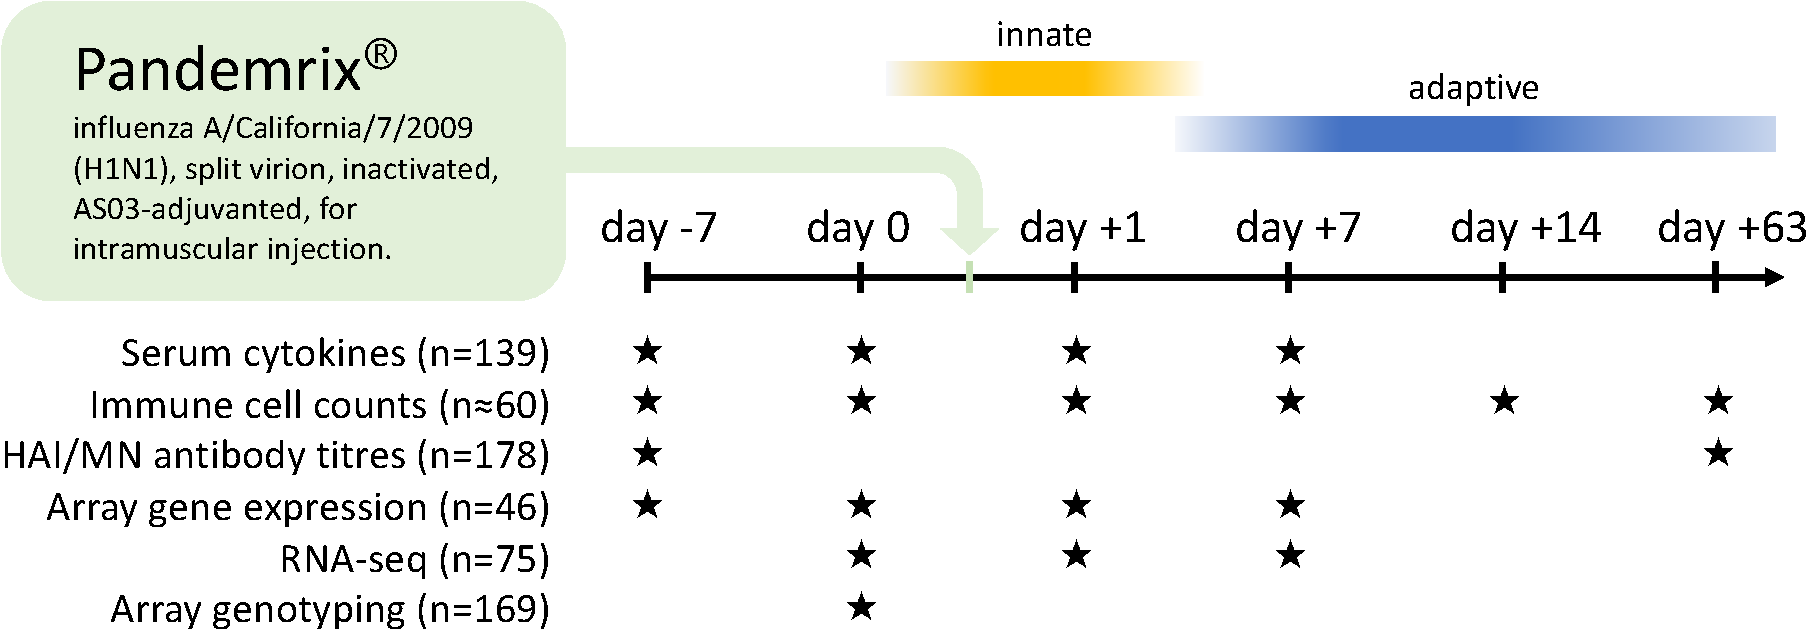
\includegraphics[width=1.0\textwidth]{mainmatter/figures/chapter_02/graphics_ashg19/hird_design-crop.pdf}
    \caption{Data types, timepoints, and sample sizes. Individuals were vaccinated after day 0 sampling. Antibodies to the vaccine strain were measured by \gls{HAI} and \gls{MN} assays. Array and \gls{RNAseq} gene expression measured in the \gls{PBMC} compartment.}
    \label{fig:hird_design}
\end{figure}

\subsection{Computing baseline-adjusted measures of antibody response}

In \autocite{sobolev2016AdjuvantedInfluenzaH1N1Vaccination}, Pandemrix responders were defined as individuals with $\ge$4-fold titre increases in either the \gls{HAI} or \gls{MN} assays.
This is a threshold for seroconversion set out by the U.S. Food and Drug Administration\autocite{foodanddrugadministration2007GuidanceIndustryClinical}, and is used in many studies of seasonal influenza vaccines\autocite{hagan2015SystemsVaccinologyEnabling}.
The responder status for 166 individuals with both \gls{HAI} and \gls{MN} titres available at baseline (day -7) and post-vaccination (day 63) were computed according to this definition.
\todo{atm I'm not using R/NR. wording here implys I am}
% \begin{outline}
% \1 Pre-process phenotypes
%     \2 Compute responder status (>= 4-fold in HAI or MN)
%     \2 Compute TRI (based on Bucasas 2009)
%         \3 “We related the change in titer between pre- and postvaccination measurements (response variable) to the prevaccination titer (explanatory variable) using a simple linear model”
%         \3 “We next determined the residuals from the above linear regressions and used them as the input values for the individual response scores.”
%         \3 “we standardized the residuals by dividing by the residual standard deviation for each component”
%             \4 Based on their axis ranges, it appears they are plotting log2(post)-log2(pre)), equivalently log2(post/pre), a.k.a. log2 fold-change; against log2(pre)
%             \4 Note that log2(post-pre) does not make sense mathematically, as post-pre may well be negative
%             \4 The negative relationship indicates lower initial titres are more amenable to high fold-change increases, which is exactly what TRI is designed to correct for
% \end{outline}
However, \autocite{sobolev2016AdjuvantedInfluenzaH1N1Vaccination} noted there was heterogeneity in the baseline titres of non-responders, citing \enquote{glass ceiling} non-responders whose high baseline titres made the fixed 4-fold threshold hard to achieve.\todo{cite appropriate subfigures here}
Dichotomisation of continuous response variables can also result in loss of statistical power \autocite{cohen1983CostDichotomization, fedorov2009ConsequencesDichotomization}.

To address these concerns, I computed the \gls{TRI} as defined in \textcite{bucasas2011EarlyPatternsGene}.
For each assay, a linear regression was fit with the $\log_2{\text{day 63}/\text{day -7}}$ titre fold change as the response, and the $\log_2{\text{day -7}}$ baseline titre as the predictor.
The residuals from the two regressions were each standardized to zero mean and unit variance, then averaged.
The \gls{TRI} expresses a continuous measure of change in antibody titres across both assays post-vaccination, compared to individuals with a similar baseline titre, and remains comparable to the binary 4-fold change definition (\autoref{fig:hird_tri}).\todo{cite appropriate subfigures here, after adding proper subfigure labels}

\begin{figure}
    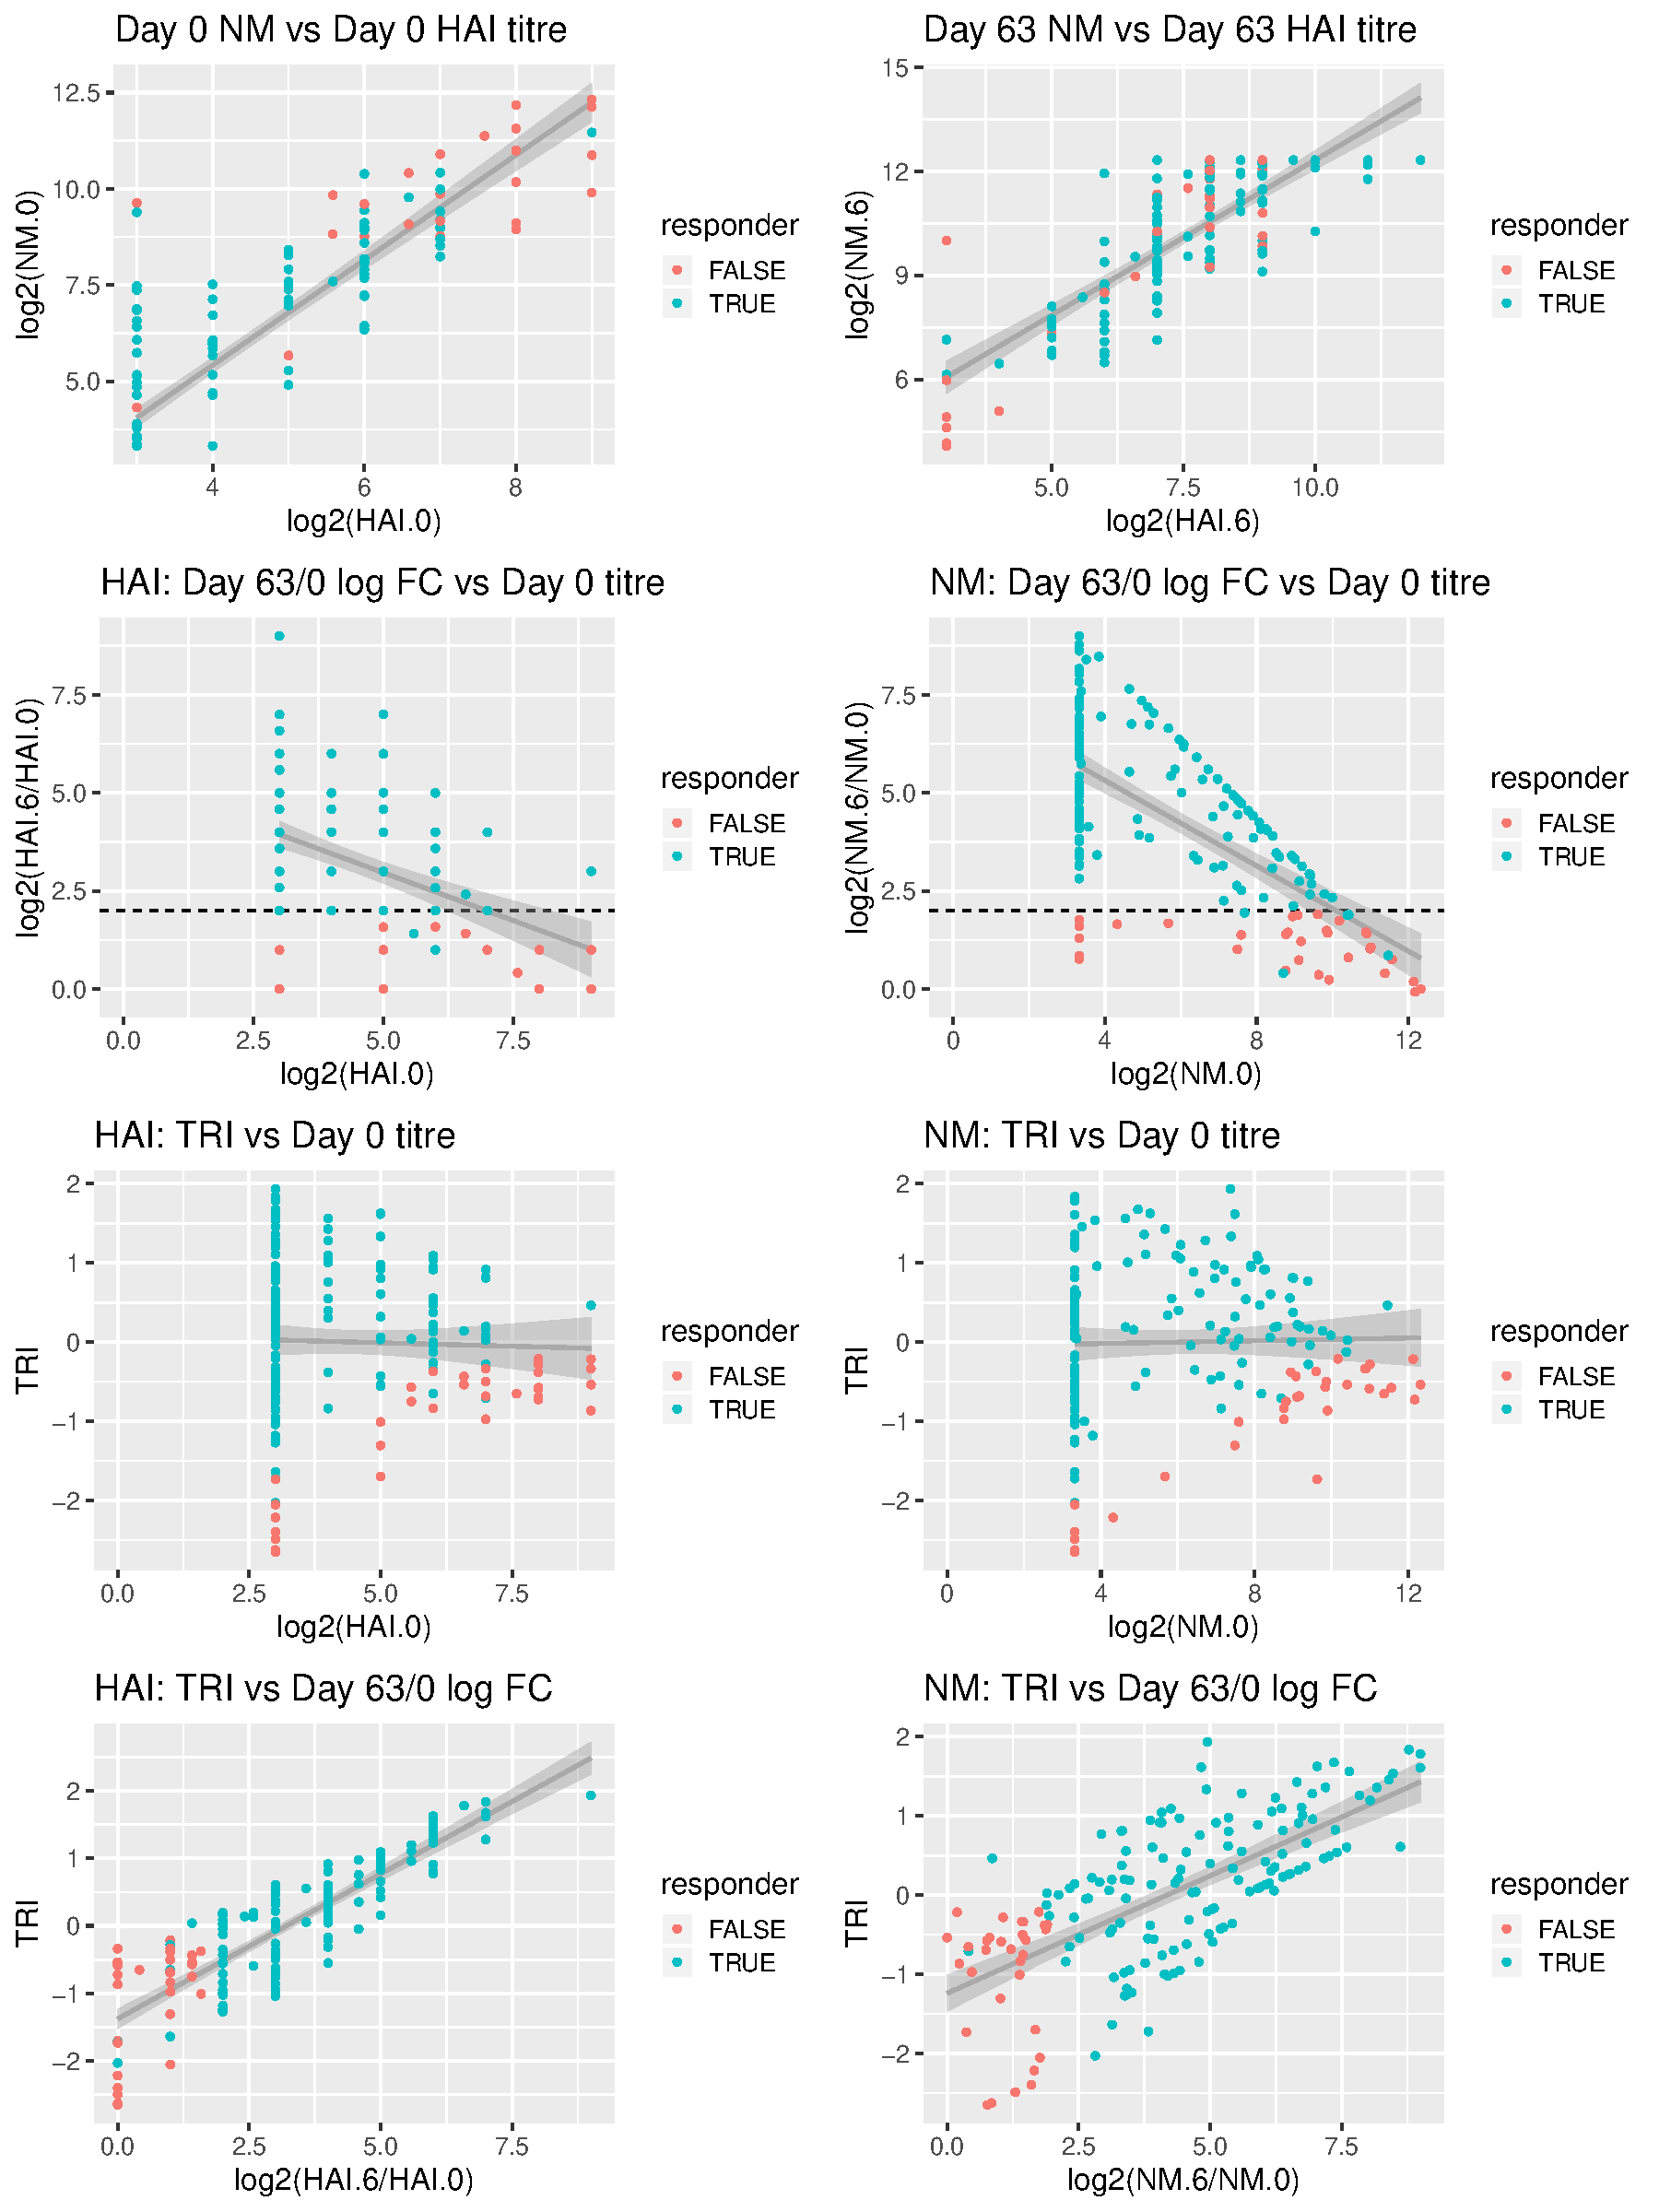
\includegraphics[width=1.0\textwidth]{mainmatter/figures/chapter_02/phenotype_data_setup.tri_comparison.pdf}
    \caption{Comparison of \gls{TRI} to \gls{HAI} (left column) and \gls{MN} (right column) titres and binary responder/non-responder status (colored) in 166 \gls{HIRD} individuals. Row 1: baseline titres are positively correlated to post-vaccination titres. Row 2: baseline titres are negatively correlated to fold change. Row 3: \gls{TRI} regresses out the correlation between baseline titre and response. Row 4: \gls{TRI} is still comparable in ordering to binary response status.}
    \label{fig:hird_tri}
\end{figure} 

Descriptive statistics for the 114 individuals with both gene expression and antibody titre data are presented in \autoref{tab:hird_table1}.
Although the proportion of responders between array (32/44) and \gls{RNAseq} (59/70) individuals is similar ($p = 0.1551$, Fisher's exact test), the variance of \gls{TRI} in array individuals is higher ($p = 0.0002098$, Levene's test), suggesting more extreme antibody response phenotypes are present (\autoref{fig:hird_phenotypes_by_platform}).
The cause of this is unknown, there is a possibility that individuals with more extreme phenotypes were prioritised for array transcriptomics in the original \gls{HIRD} study\footnote{Personal communication with authors.}.

\begin{table}[] 
 \centering 
 \caption{\textbf{Descriptive statistics for individuals with both expression and antibody data.} Values are count and percentage for categorial variables; mean and standard deviation for continuous variables. P values are for the comparison between platforms.}\label{tab:hird_table1}
 \begin{tabular}{ l c c c }
 \toprule
  &   &  \multicolumn{ 2 }{c}{ Platform }\\ 
  & Total & Array & \gls{RNAseq} \\ 
  & n = 114 & n = 44 & n = 70 \\ 
  \midrule
 Gender &   &   &  \\ 
 \hspace{6pt}    F & 72 (63.2\%) & 27 (61.4\%) & 45 (64.3\%)\\ 
 \hspace{6pt}    M & 42 (36.8\%) & 17 (38.6\%) & 25 (35.7\%)\\ 
 Age at vaccination (years)  &   &   &  \\ 
 \hspace{6pt}   & 29.2 (11.8) & 32.9 (14.1) & 26.8 (9.4)\\ 
 Ancestry (self-reported) &   &   &  \\ 
 \hspace{6pt}    Asian & 14 (12.3\%) & 5 (11.4\%) & 9 (12.9\%)\\ 
 \hspace{6pt}    Black/African & 9 (7.9\%) & 4 (9.1\%) & 5 (7.1\%)\\ 
 \hspace{6pt}    Caucasian & 82 (71.9\%) & 33 (75\%) & 49 (70\%)\\ 
 \hspace{6pt}    Latin American & 2 (1.8\%) & 1 (2.3\%) & 1 (1.4\%)\\ 
 \hspace{6pt}    Mixed & 5 (4.4\%) & 1 (2.3\%) & 4 (5.7\%)\\ 
 \hspace{6pt}    Other - Arab & 1 (0.9\%) & 0 (0\%) & 1 (1.4\%)\\ 
 \hspace{6pt}    White Other & 1 (0.9\%) & 0 (0\%) & 1 (1.4\%)\\ 
 log2 day -7 HAI  &   &   &  \\ 
 \hspace{6pt}   & 4.4 (1.8) & 4.2 (1.6) & 4.5 (1.9)\\ 
 log2 day 63 HAI  &   &   &  \\ 
 \hspace{6pt}   & 7.6 (1.8) & 7.4 (2.2) & 7.6 (1.5)\\ 
 log2 HAI fold change  &   &   &  \\ 
 \hspace{6pt}   & 3.2 (1.9) & 3.2 (2.4) & 3.1 (1.6)\\ 
 log2 day -7 MN  &   &   &  \\ 
 \hspace{6pt}   & 6.2 (2.8) & 5.4 (2.4) & 6.6 (3.0)\\ 
 log2 day 63 MN  &   &   &  \\ 
 \hspace{6pt}   & 10.4 (2.0) & 9.5 (2.2) & 10.9 (1.6)\\ 
 log2 MN fold change  &   &   &  \\ 
 \hspace{6pt}   & 4.2 (2.3) & 4.1 (2.6) & 4.3 (2.1)\\ 
 Responder (binary definition) &   &   &  \\ 
 \hspace{6pt}    FALSE & 23 (20.2\%) & 12 (27.3\%) & 11 (15.7\%)\\ 
 \hspace{6pt}    TRUE & 91 (79.8\%) & 32 (72.7\%) & 59 (84.3\%)\\ 
 TRI &   &   &  \\ 
 \hspace{6pt}   & -0.0 (0.9) & -0.2 (1.2) & 0.1 (0.7)\\ 
 \bottomrule
 
 \end{tabular}
 \end{table}


\begin{figure}
    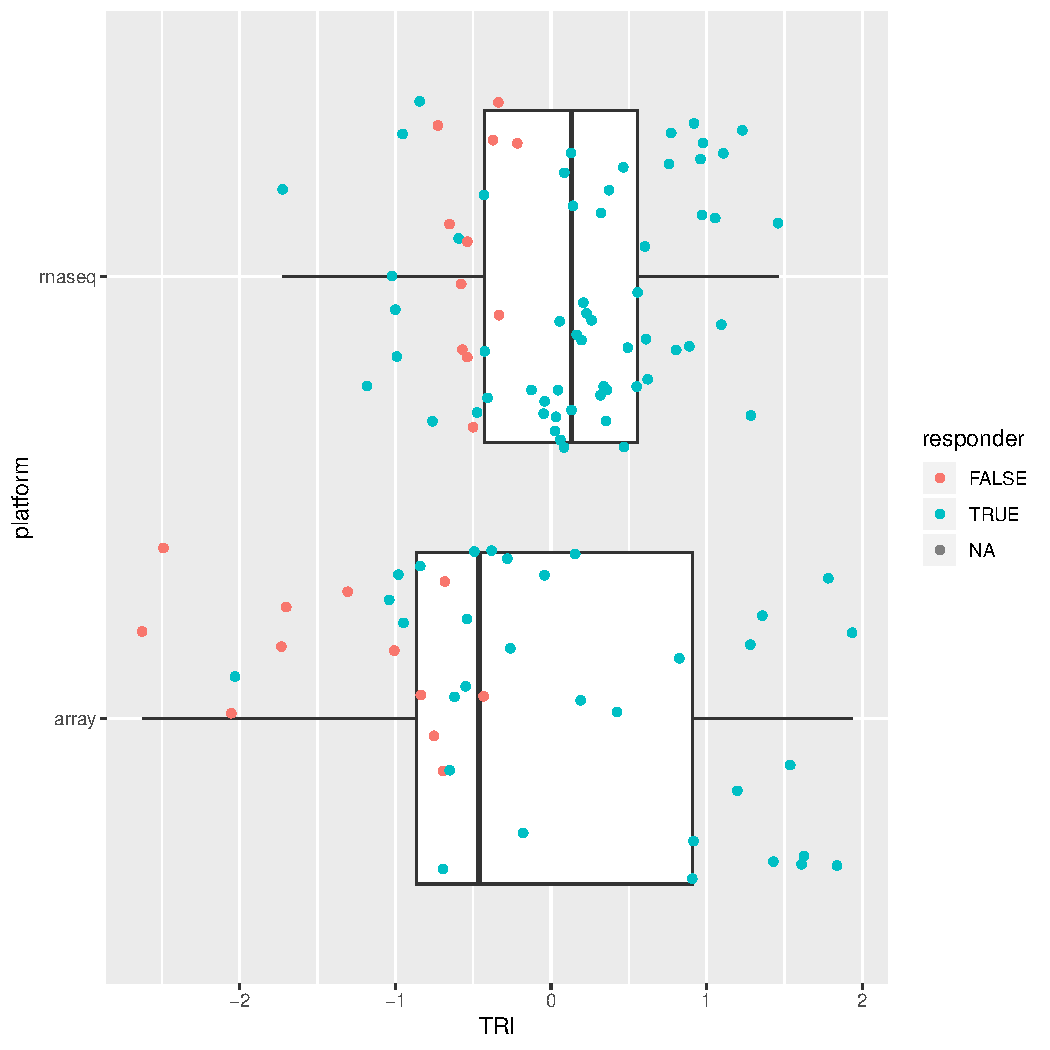
\includegraphics[width=1.0\textwidth,page=1]{mainmatter/figures/chapter_02/compare_phenotype_by_platform.pheno_boxplots.pdf}
    \caption{Distribution of \gls{TRI}, stratified by platform used to measure expression.}
    \label{fig:hird_phenotypes_by_platform}
\end{figure}

\subsection{Genotype data generation}

\todo{Add to collab note that extractions were done at KCL}
DNA was extracted from frozen blood using the Blood and Tissue DNeasy kit (Qiagen), and genotyping was performed using on the Infinium CoreExome-24 BeadChip (Illumina).
In total, 192 samples from 176 individuals in the HIRD cohort were genotyped at 550601 markers, including replicate samples submitted for individuals where extracted DNA concentrations were low.

\subsection{Genotype data preprocessing}
\label{subsec:hird_dge_genotype_preproc}

Using PLINK (v1.90b3w), genotype data underwent the following quality control procedures to remove poorly genotyped samples and markers:
max marker missingness across samples $< 5\%$, 
max sample missingness across markers $< 1\%$, 
max marker heterozygosity rate within 3 standard deviations of the mean (threshold selected visually to exlude outliers, \autoref{fig:hird_genotype_sample_hetRate_missingness}),
% The HWE threshold should depend on the multi-ethnicity of the cohort
removal of markers that deviate from Hardy–Weinberg equilibrium (\texttt{-{}-hwe} option, $\text{p} < 0.00001$).

\begin{figure}
    \includegraphics[width=1.0\textwidth,page=2]{mainmatter/figures/chapter_02/coreex_eQTLflu_20171204.gencall.smajor.impute_sex.qc2.pdf}
    \caption{Sample filters for missingness and heterozygosity rate. Samples outside the central rectangle were excluded.}
    \label{fig:hird_genotype_sample_hetRate_missingness}
\end{figure}

To exclude highly-related individuals and deduplicate replicate samples, pairwise kinship coefficients were computed on \gls{MAF} $< 0.05$ pruned genotypes using KING (v1.4).
For each pair of samples with pairwise kinship coefficient $> 0.177$ (first-degree relatives or closer), the sample with lower marker missingness was selected.

After filtering, 169 samples and 549414 markers remained.

\subsection{Computing genotype \glsfmtlongpl{PC} as covariates for ancestry}
\label{subsec:hird_dge_genotype_pc}

As shown in \autoref{tab:hird_table1}, the \gls{HIRD} cohort is multi-ethnic, hence there is potential for confounding by population structure (sample structure due to genetic ancestry) in expression and genetic association studies \autocite{price2006PrincipalComponentsAnalysis,eu-ahsunthornwattana2014ComparisonMethodsAccount,brown2018ExpressionReflectsPopulation}.
Treating HapMap 3 samples as a reference population where the major axes of variation in genotypes are likely to be ancestry, \gls{PCA} was performed using smartpca (v8000) on \gls{LD}-pruned genotypes (\texttt{PLINK -{}-indep-pairwise 50 5 0.2}).
\gls{HIRD} sample \glspl{PC} were computed by projection onto the HapMap 3 \gls{PCA} eigenvectors.
For non-genotyped individuals, \gls{PC} values were imputed as the mean value for all genotyped individuals with the same self-reported ancestry.
The top \glspl{PC} separate samples of European, African and Asian ancestry (\autoref{fig:hird_genotype_pca_withHapmap}), hence these \glspl{PC} can be used as covariates for ancestry downstream.
\todo{Add Tracy-Widom statistics for PCs to justify later choice of 4 PCs for covariates}
\todo{nicer version, copy the peer code, facet the hird and hapmap samples}

\begin{figure}
    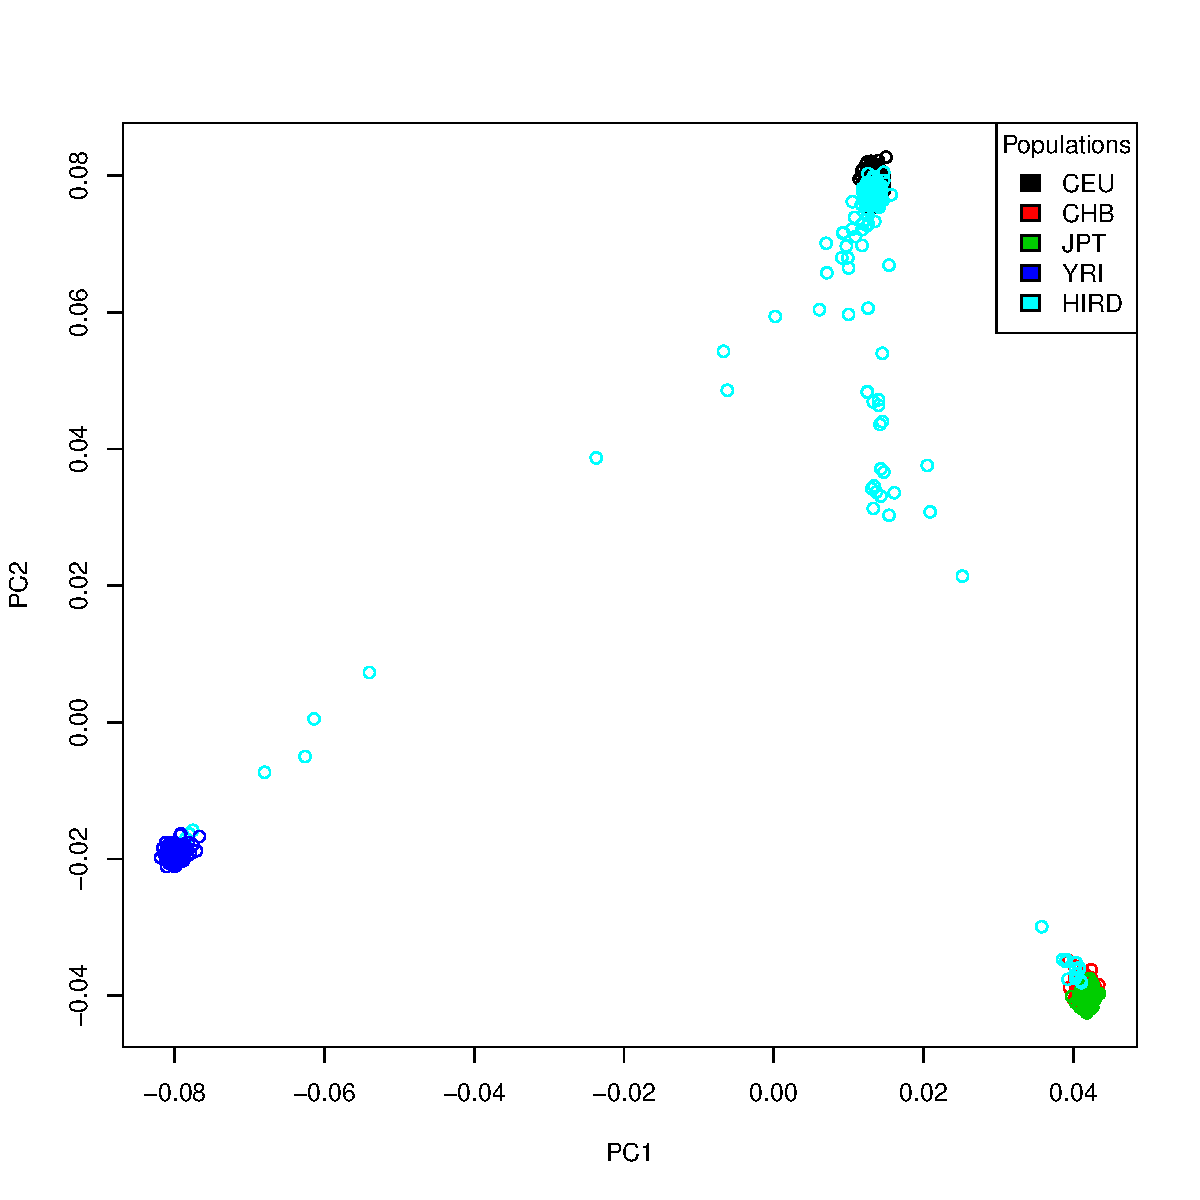
\includegraphics[width=1.0\textwidth]{mainmatter/figures/chapter_02/coreex_eQTLflu_20171204.gencall.smajor.impute_sex.qc3.pruned.hapmap_merged.flipped.pca.evec.pdf}
    \caption{\gls{HIRD} samples (cyan) projected onto \gls{PC}1 and \gls{PC}2 axes defined by \gls{PCA} of HapMap 3 samples. The first two \glspl{PC} separate European (CEU, upper-right) from Asian (CHB and JPT, lower-right) and African (YRI, lower-left) individuals.}
    \label{fig:hird_genotype_pca_withHapmap}
\end{figure}

\subsection{\glsfmtshort{RNAseq} data generation}

Total RNA was extracted from \glspl{PBMC} using the Qiagen RNeasy Mini kit, with on-column DNase treatment.
RNA integrity was checked on the Agilent Bioanalyzer and mRNA libraries were prepared with the KAPA Stranded mRNA-Seq Kit (KK8421), which uses poly(A) selection.
% 7 lanes x 3 plates
To avoid confounding of timepoint and batch effects from pooling, samples were pooled by library prep plate, ensuring libraries from all timepoints of an individual were in the same pool, and then sequenced across multiple lanes as technical replicates (HiSeq 4000, 75bp paired-end).

% To get to cram files:
% From .cram headers:
% 1.	The NextSeq, HiSeq, and NovaSeq Sequencing Systems generate raw data files in binary base call (BCL) format.
% 1.1.	HiSeq Sequencing Control Software (SCS), version HD 3.4.0.38, used for basecalling
% 2.	biobambam2/bamadapterfind: bamdapterfind scans a BAM file for contaminations by sequencing adapters.
% 3.	bambi decode: decode a multiplexed bam file
% 4.	bwa sampe (alignment using BWA-backtrack): alignment to phiX, which is then merged with the original bam
% 5.	pb_calibration/spatial_filter: Identify regions with spatially correlated errors e.g. bubbles, (from aligned BAM files where the read name can be parsed for spatial location) and allow filtering out or marking of the BAM fail bit for reads in those regions.
% 6.	Alignment with tophat 2.0.14
% 6.1.	 --keep-fasta-order --no-sort-bam --output-dir tophat_out_24165_1#10 --mate-inner-dist 100 --num-threads=8 --library-type=fr-firststrand --no-coverage-search --microexon-search --transcriptome-index=/lustre/scratch117/core/sciops_repository/transcriptomes/Homo_sapiens/ensembl_83_transcriptome/GRCh38_15_plus_hs38d1/tophat2/GRCh38_15_plus_hs38d1.known/lustre/scratch117/core/sciops_repository/references/Homo_sapiens/GRCh38_15_plus_hs38d1/all/bowtie2/Homo_sapiens.GRCh38_15_plus_hs38d1.fa
% 7.	Some sort of duplicate marking and filtering (?) using some combination of:
% 7.1.	biobambam/bamsormadup: parallel sorting and duplicate marking
% 7.2.	uk.ac.sanger.npg.picard.AlignmentFilter
% 7.3.	biobambam/bamstreamingmarkduplicates
% 8.	Write .cram files using scramble (cram is a reference-based compression)
% 8.1.	/lustre/scratch117/core/sciops_repository/references/Homo_sapiens/GRCh38_15_plus_hs38d1/all/fasta/Homo_sapiens.GRCh38_15_plus_hs38d1.fa
% 9.	NOTE: Note lots of intermediate biobambam 2.0.76 and scramble processing steps, not all are listed.

\todo{Can add other fastqc plots e.g. kmers, overrepresented seqs, seq length}
% Genomic origin of reads and gene end biases were assessed using Qualimap, after aligning the reads to the human GRCh38_15_plus_hs38d10 reference transciptome using tophat2.
\gls{RNAseq} quality metrics were assessed using FASTQC\footnote{\url{https://www.bioinformatics.babraham.ac.uk/projects/fastqc/}} and Qualimap\autocite{okonechnikov2015QualimapAdvancedMultisample}, then visualised with MultiQC\autocite{ewels2016MultiQCSummarizeAnalysis}.
% See log 2017-11-20 for fastqc discussion
Sequence quality was high (\autoref{fig:hird_fastqc_seqQual}), and duplication levels were low (\autoref{fig:hird_fastqc_seqDupe}).
The unimodal GC-content distribution suggested negligible levels of non-human contamination (\autoref{fig:fastqc_gc}).

\begin{figure}
	\centering
	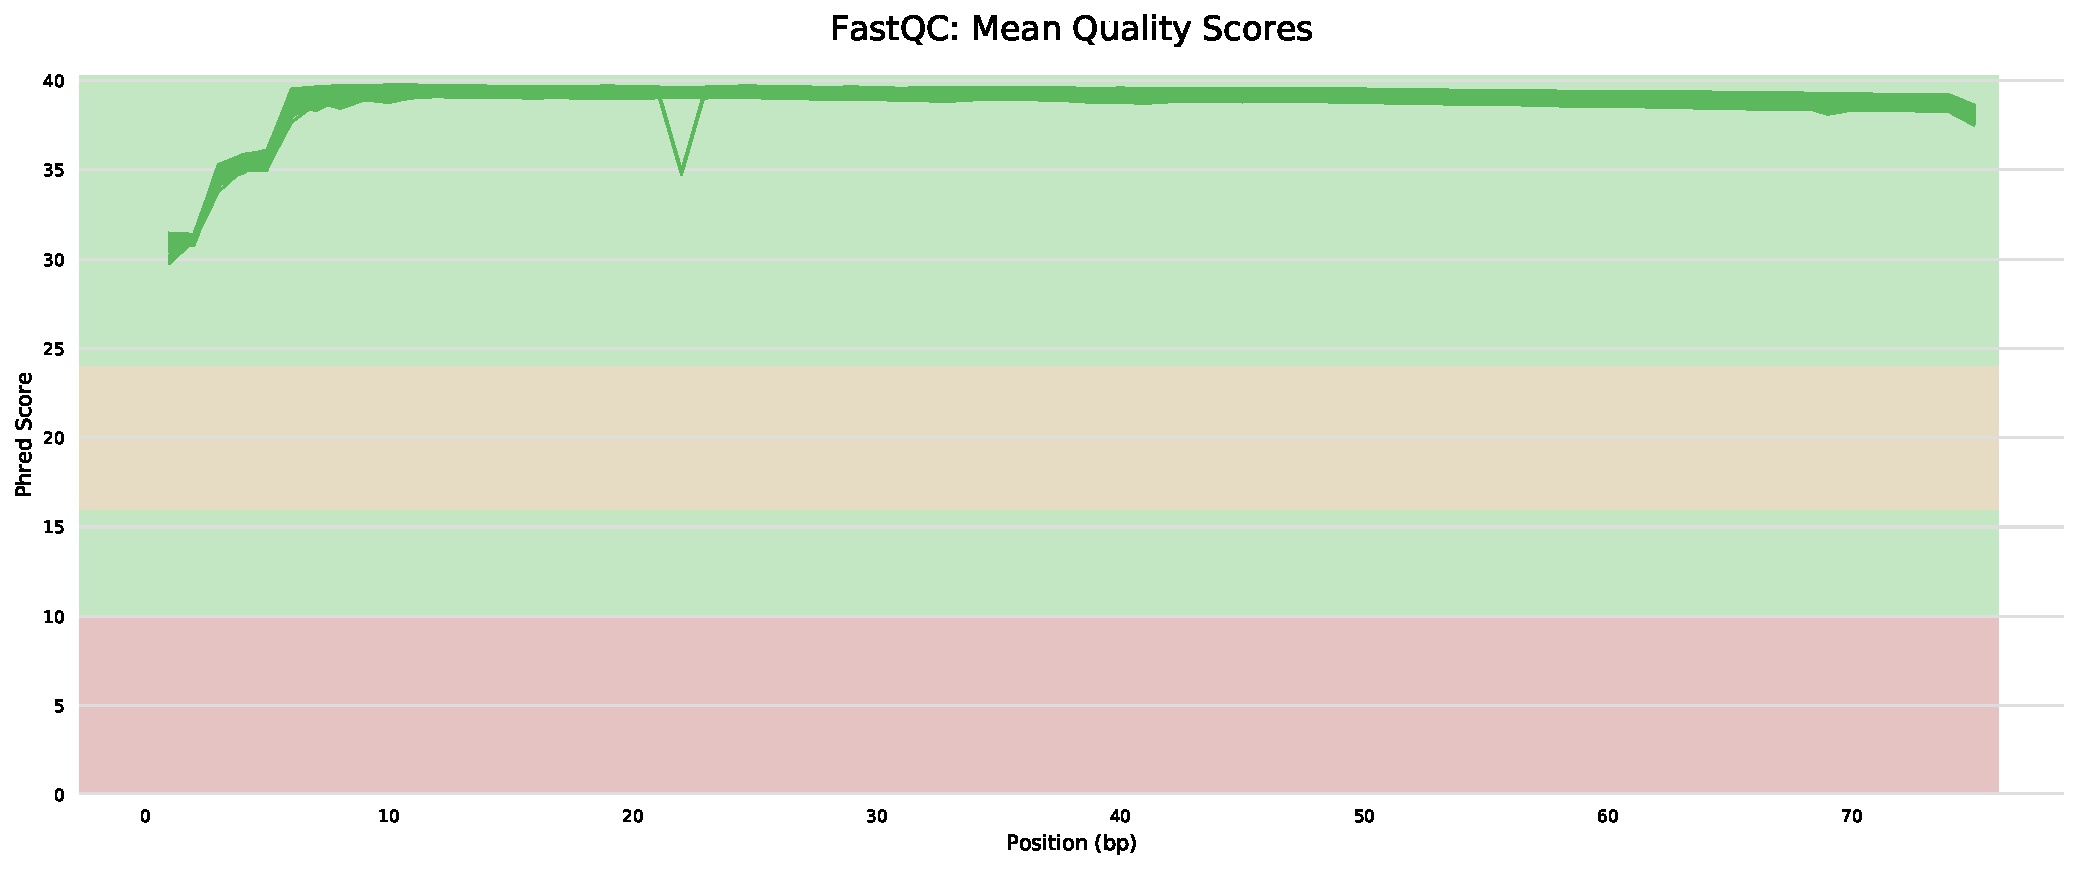
\includegraphics[width=\textwidth]{mainmatter/figures/chapter_02/graphics_firstYearReport/fastqc/mqc_fastqc_per_base_sequence_quality_plot_1.pdf}
    \caption{FastQC sequence quality versus read position for \gls{HIRD} \gls{RNAseq} samples.}
	\label{fig:hird_fastqc_seqQual}
\end{figure}

\begin{figure}
	\centering
	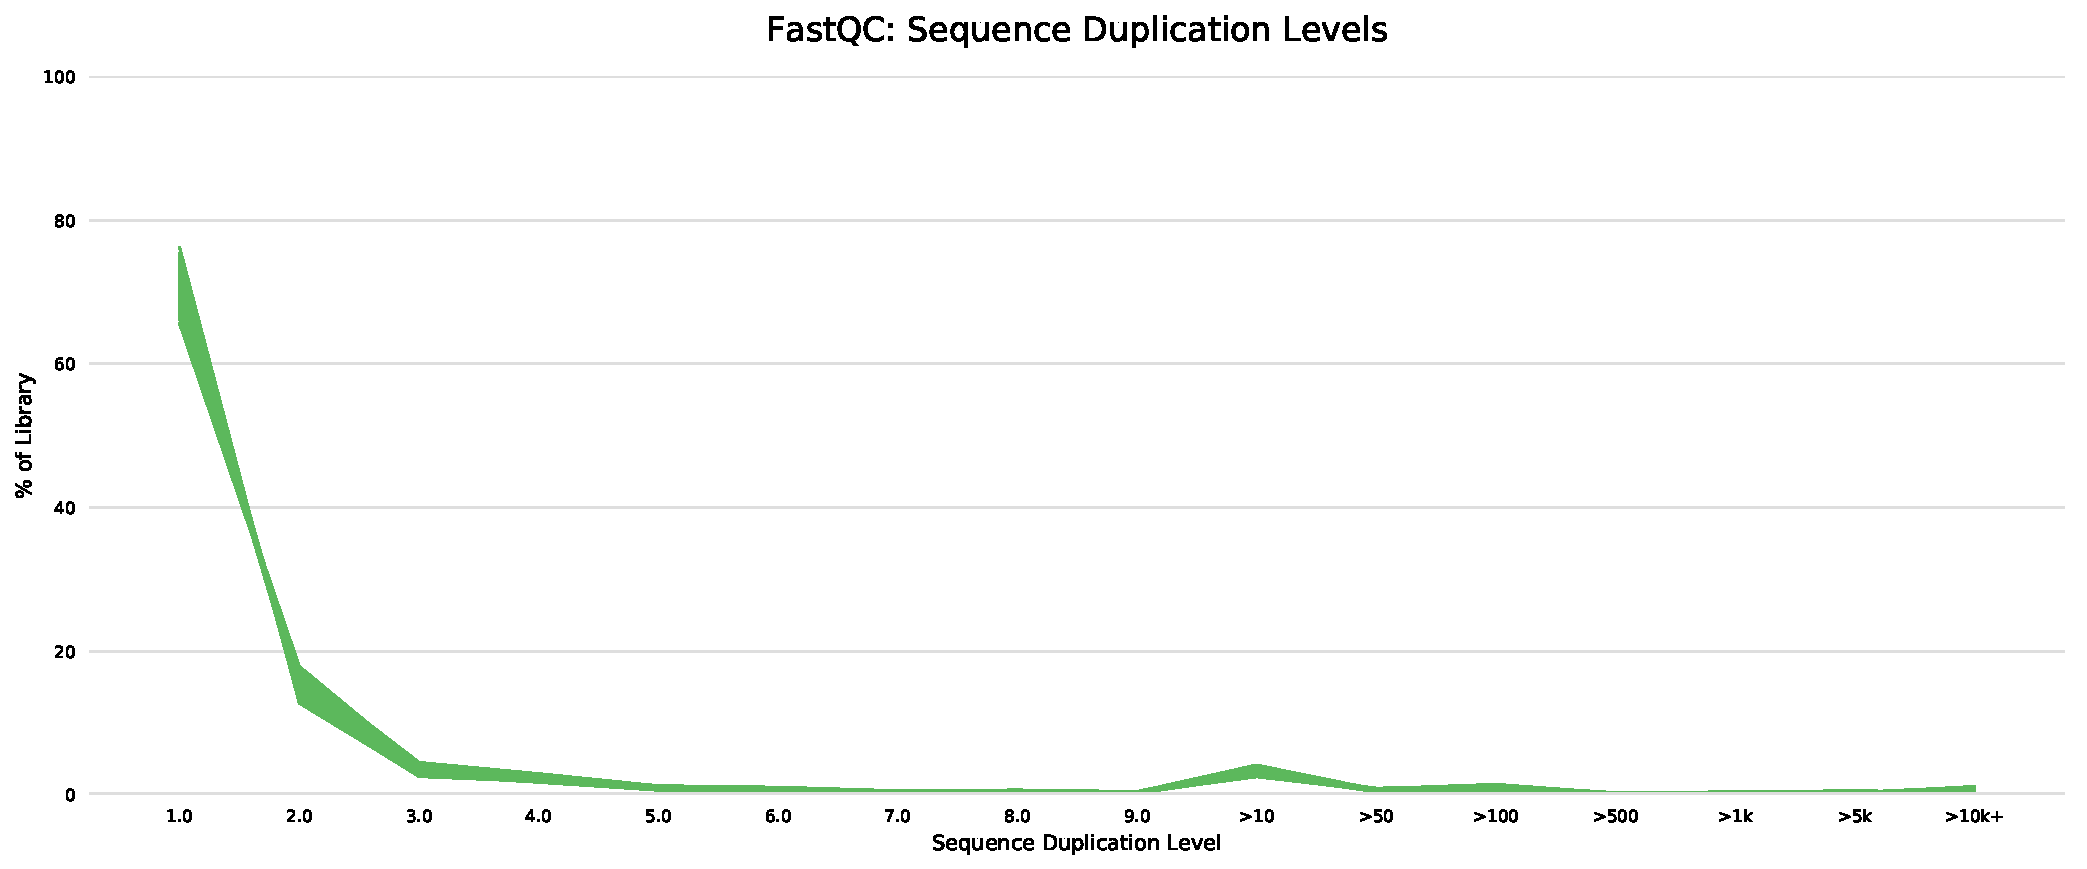
\includegraphics[width=\textwidth]{mainmatter/figures/chapter_02/graphics_firstYearReport/fastqc/mqc_fastqc_sequence_duplication_levels_plot_1.pdf}
	\caption{FastQC sequence duplication levels for \gls{HIRD} \gls{RNAseq} samples.}
	\label{fig:hird_fastqc_seqDupe}
\end{figure}

\begin{figure}
	\centering
	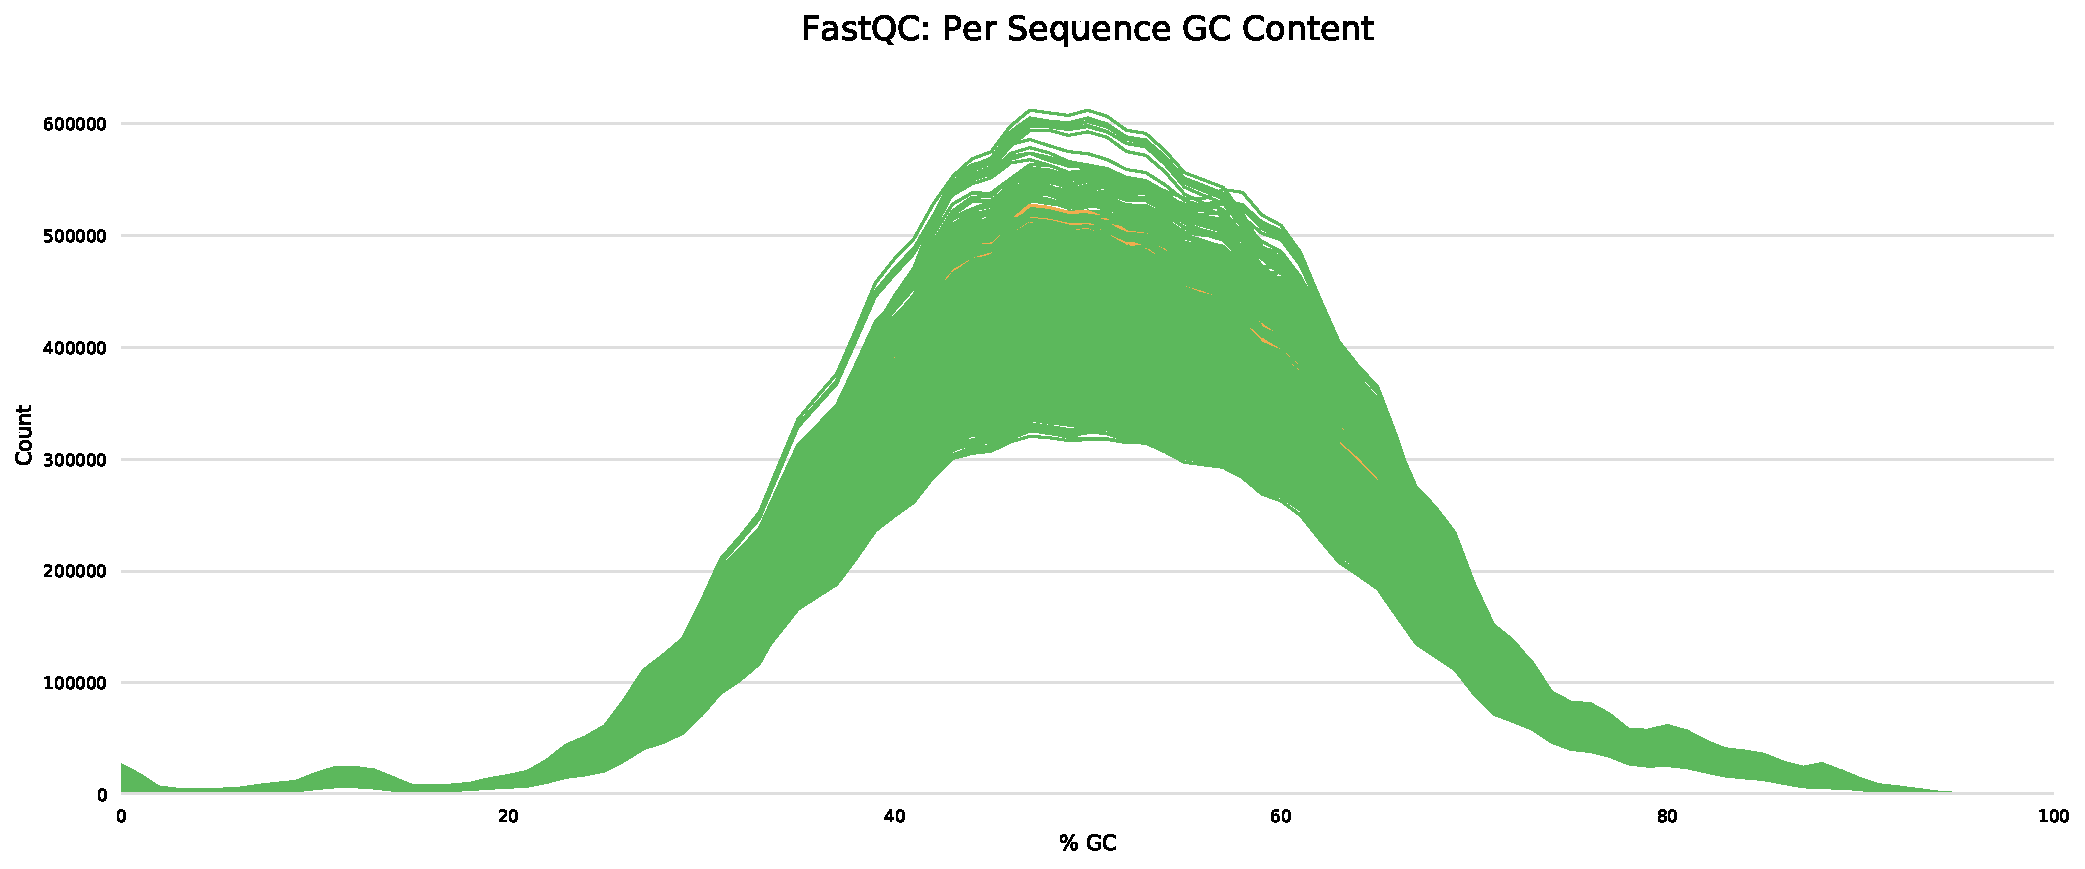
\includegraphics[width=\textwidth]{mainmatter/figures/chapter_02/graphics_firstYearReport/fastqc/mqc_fastqc_per_sequence_gc_content_plot_Counts.pdf}
	\caption{FastQC GC profile for \gls{HIRD} \gls{RNAseq} samples.}
	\label{fig:fastqc_gc}
\end{figure}

\subsection{\glsfmtshort{RNAseq} quantification and filtering}
\label{subsec:hird_dge_rnaseq_quantAndFilter}

% 1.	Quantification (Salmon --libType ISR, which is equiv to TopHat -fr-firststrand with paired end data)
% 1.1.	Used index /lustre/scratch117/core/sciops_repository/transcriptomes/Homo_sapiens/ensembl_83_transcriptome/GRCh38_15_plus_hs38
% 1.1.1.	This is GRCh38.p5, Dec 2017, v83; with additional hs38d1: Decoy version 1 for GRCh38
% 1.1.2.	Contains ENST transcript ids
% 1.2.	Output quantifies transcripts in terms of: TPM — This is salmon’s estimate of the relative abundance of this transcript in units of Transcripts Per Million (TPM). TPM is the recommended relative abundance measure to use for downstream analysis.
% 1.2.1.	https://haroldpimentel.wordpress.com/2014/05/08/what-the-fpkm-a-review-rna-seq-expression-units/ TPM = (count/effectiveLength) / sumOverAllTranscripts(count/effectiveLength)
% 1.3.	Note Salmon also takes into account: EffectiveLength — This is the computed effective length of the target transcript. It takes into account all factors being modeled that will effect the probability of sampling fragments from this transcript, including the fragment length distribution and sequence-specific and gc-fragment bias (if they are being modeled).
% 2.	Gene-level regeneration of counts (tximport)
% 2.1.	“generate estimated counts using abundance estimates scaled up to library size (scaledTPM)”
% 2.1.1.	Note, we do not scale for gene length, that would be lengthScaledTPM. Hence the generated counts remain length-corrected.
% 2.2.	Summarizes using a mapping of ENST to ENSG, generated from /lustre/scratch117/core/sciops_repository/transcriptomes/Homo_sapiens/ensembl_83_transcriptome/GRCh38_15_plus_hs38d1/gtf/ensembl_83_transcriptome-GRCh38_15_plus_hs38d1.gtf
% 2.3.	Counts from all lanes of a sample are summed
% 3.	GC bias, length bias, mappability
% 3.1.	Length bias only affects RNAseq: somewhat alleviated by Salmon using effective length
% 3.2.	GC bias affects both technologies: somewhat alleviated by Salmon using effective length (see the salmon paper)
% NOTE:
% 3.3.	Mappability has not been considered
\todo{add software versions}
Reads were quantified against the Ensembl reference transcriptome (GRCh38) using Salmon\autocite{patro2017SalmonProvidesFast} in quasi-mapping-based mode, which internally accounts for transcript length and GC composition.
% https://www.biostars.org/p/304552/
To combine technical replicates, as the sum of Poisson distributions remains Poisson-distributed, counts for technical replicates were summed for each sample.
% Also see:
%
% https://genomebiology.biomedcentral.com/articles/10.1186/s13059-016-0881-8
% "While some authors will argue that as few as five million mapped reads are sufficient to quantify accurately medium to highly expressed genes in most eukaryotic transcriptomes, others will sequence up to 100 million reads to quantify precisely genes and transcripts that have low expression levels [7]."
%
% https://genome.ucsc.edu/ENCODE/protocols/dataStandards/ENCODE_RNAseq_Standards_V1.0.pdf
% 2. Sequencing depth.
% The amount of sequencing needed for a given sample is determined by the goals of the experiment and the nature of the RNA sample.
% Experiments whose purpose is to evaluate the similarity between the transcriptional profiles of two polyA+ samples may require only modest depths of sequencing (e.g. 30M pair-end reads of length > 30NT, of which 20-25M are 3mappable to the genome or known transcriptome, Experiments whose purpose is discovery of novel transcribed elements and strong quantification of known transcript isoforms requires more extensive sequencing.
% The ability to detect reliably low copy number transcripts/isoforms depends upon the depth of sequencing and on a sufficiently complex library.
% For experiments from a typical mammalian tissue or in which sensitivity of detection is important, a minimum depth of 100-200 M 2 x 76 bp or longer reads is currently recommended.
The mean number of mapped read pairs per sample after summing was 27.09 million read pairs (range 20.24-39.14 million), representing a mean mapping rate of 80.73\% (range 75.57-90.10\%), comfortably within sequencing depth recommendations for \gls{DGE} experiments\autocite{liu2014RNAseqDifferentialExpression}.
Relative transcript abundances were summarised to Ensembl gene-level count estimates using tximport (scaledTPM method) to improve statistical robustness and interpretability\autocite{soneson2016DifferentialAnalysesRNAseq}.

% 5.	Pre-process RNA-seq expression data
% 5.1.	Pull in tximport counts
% 5.1.1.	60675 loci, 223 samples
% 5.2.	Add gene annotation based on EnsDb.Hsapiens.v86
% 5.3.	Low-count filtering (>0.5 CPM in 10% of 223 samples i.e. 22 samples)
% Max zero prop: need to be stringent as limma doesn't account for neg bin
% 5.4.	Remove globin genes and short non-coding RNAs
% 5.4.1.	Human globins: https://en.wikipedia.org/wiki/Globin#Examples
% 5.4.2.	Short non-coding GENEBIOTYPES: https://www.gencodegenes.org/pages/biotypes.html
% 5.5.	NOTE: we have not yet removed GENEBIOTYPE=NA. These may be retired ids.
Genes with short noncoding RNA biotypes\footnote{miRNA, miRNA\_pseudogene, miscRNA, miscRNA pseudogene, Mt rRNA, Mt tRNA, rRNA, scRNA, snlRNA, snoRNA, snRNA, tRNA, tRNA\_pseudogene. List from \url{https://www.ensembl.org/Help/Faq?id=468}} were removed, as they are generally not polyadenylated, and expression estimates can be biased by misassignment of counts from overlapping protein-coding or lncRNA genes\autocite{zhao2018EvaluationTwoMain}.
% Also, they can be shorter than the 75 bp read length
Globin genes, which are highly expressed in erythrocytes and reticulocytes, cell types expected to be depleted in \gls{PBMC} \autocite{min2010VariabilityGeneExpression}, were also removed.
Given the proportion of removed counts at this stage was low for most samples (\autoref{fig:hird_shortncRNA_and_globins}), poly(A) selection and \gls{PBMC} isolation procedures were deemed to have been efficient.

\begin{figure}
    \centering
    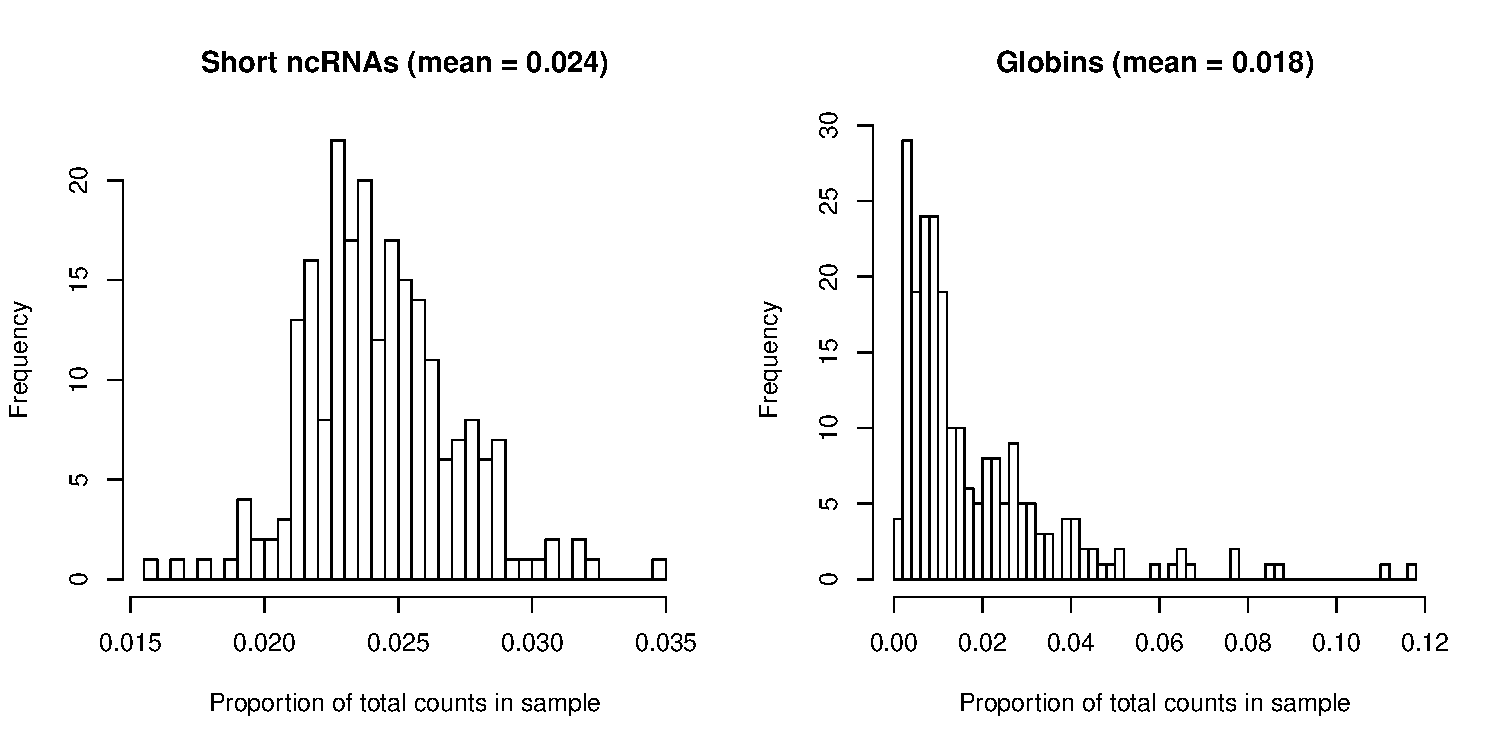
\includegraphics[width=1.0\textwidth, page=1]{mainmatter/figures/chapter_02/rnaseq_data_setup.per_sample.short_ncRNA_globin_levels_hist.pdf}
    \caption{Distributions of removed short ncRNA and globin counts as a proportion of total counts in \gls{RNAseq} samples.}
    \label{fig:hird_shortncRNA_and_globins}
\end{figure}

Many of the genes in the reference transcriptome are not expressed in \gls{PBMC} (\autoref{fig:hird_rnaseq_filtering_zeroProp}), and many genes are expressed at counts too low for statistical analysis of \gls{DGE}
Genes were further filtered to require detection (non-zero expression) in at least 95\% of samples, and a minimum of 0.5 \gls{CPM} in at least 20\% of samples.
The 0.5 \gls{CPM} threshold was chosen to correspond to approximately 10 counts in the smallest library, where 10-15 counts is a rule of thumb for considering a gene to be robustly expressed\autocite{chen2016ReadsGenesPathways}.
The change in the distribution of gene expressions among samples before and after filtering shows a substantial number of low expression genes are removed (\autoref{fig:hird_rnaseq_cpm_filtering}).

\begin{figure}
    \centering
    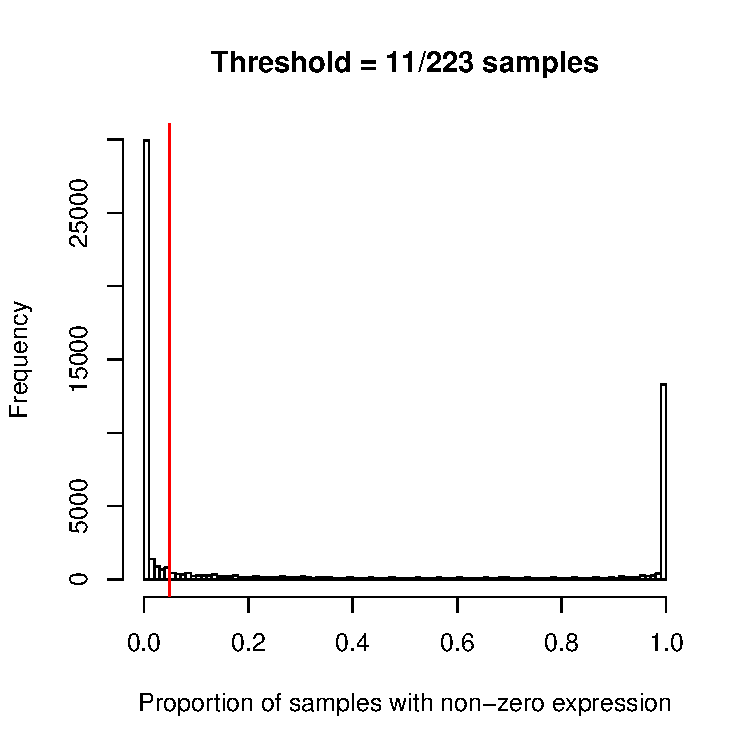
\includegraphics[width=0.6\textwidth, page=1]{mainmatter/figures/chapter_02/rnaseq_data_setup.gene_zero_prop.pdf}
    \caption{Distribution of the proportion of samples in which genes were detected (non-zero expression). Many genes are not detected in any samples. Vertical line shows 5\% threshold below which genes were discarded.}
    \label{fig:hird_rnaseq_filtering_zeroProp}
\end{figure}

\begin{figure}
    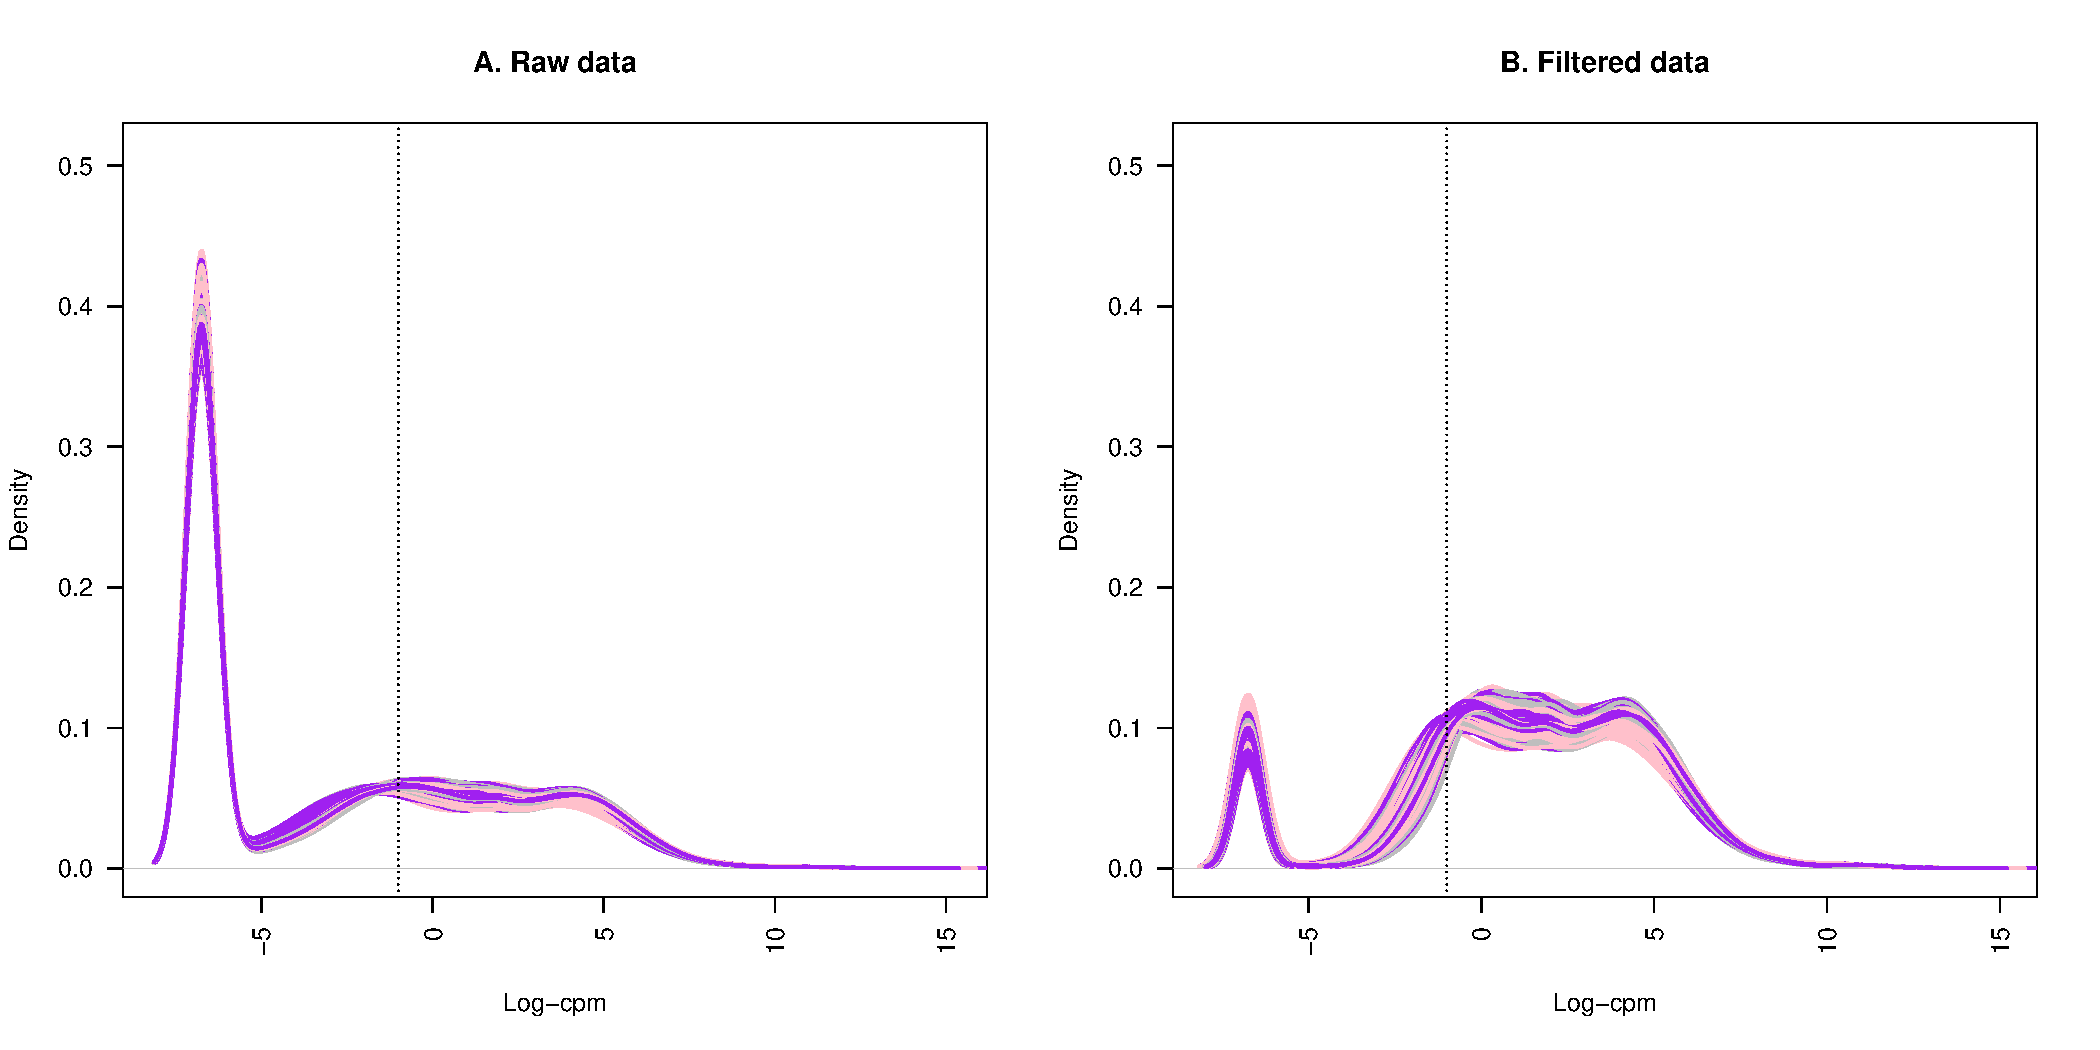
\includegraphics[width=1.0\textwidth]{mainmatter/figures/chapter_02/rnaseq_data_setup.sample_cpm_density_filtered.pdf}
    \caption{Distribution of gene expressions for \gls{RNAseq} samples before and after filtering no expression and low expression genes. Vertical line shown at \gls{CPM} = 0.5 threshold.}
    \label{fig:hird_rnaseq_cpm_filtering}
\end{figure}

After the application of all filters, expression values were available for 21626 genes over 223 samples (75/75 individuals on day 0, 73/75 on day 1, and 75/75 on day 7).

\subsection{Array data preprocessing}
\label{subsec:hird_dge_array_preproc}

% 6.	Pre-process microarray expression data
% 6.1.	Annotate Entrez and ENS ids using hgug4112a.db
% 6.1.1.	The chip is single-channel “Agilent-014850 Whole Human Genome Microarray 4x44K G4112F”
% 6.1.2.	Apparently fine to use 4112A db for 4112F https://support.bioconductor.org/p/73193/
% 6.2.	Redefine responder phenotype to be consistent with RNA-seq and Sobolev paper (>= 4-fold in HAI or MN)
% 6.3.	Background correction: limma::backgroundCorrect(x, method="normexp")
% 6.3.1.	Background comes from non-specific binding
% 6.3.2.	Pipeline from the Agi4x44PreProcess Bioconductor package (deprecated)
% 6.3.3.	Notes on Edwards: https://academic.oup.com/bioinformatics/article/23/20/2700/230165#2633725
% 6.3.3.1.	“adjusts the foreground intensities by subtracting the background when the difference between the foreground and background is larger than a small threshold value. When the difference is less than the threshold, subtraction is replaced by a smooth monotonic function.“
% 6.3.3.2.	May be preferred over normexp in our case due to “Question: Compressed boxplots after 'normexp+offset' background correction of Agilent one color microarrays in LIMMA“ https://support.bioconductor.org/p/46485/
% 6.3.3.3.	Example of Edwards used over normexp for Agilent arrays: “Modified least-variant set normalization for miRNA microarray” https://www.ncbi.nlm.nih.gov/pmc/articles/PMC2995391/
% 6.3.3.4.
% 6.3.4.	Notes on normexp:
% 6.3.4.1.	This function is designed to produce positive corrected intensities.
% 6.3.4.1.1.	“If the "normexp" method is selected, then a convolution of normal and exponential distributions is fitted to the foreground intensities using the background intensities as a covariate, and the expected signal given the observed foreground becomes the corrected intensity.”
% 6.3.4.1.2.	https://www.ncbi.nlm.nih.gov/pmc/articles/PMC2648902/ “A method normexp was introduced which models the observed intensities as the sum of exponentially distributed signals and normally distributed background values”
% 6.3.4.2.	[…] an offset value (normally 50) is used. This offset adds a constant to the intensities before log-transforming, so that the log ratios are shrunk towards zero at the lower intensities.
% 6.3.4.3.	The optimal choice for the offset is the one which makes the variability of the log-ratios as constant as possible across the range of intensity values (Smyth, G. in BioC mailing List, https://stat.ethz.ch/pipermail/bioconductor/2006-April/012554.html ).
% 6.3.5.	Choice of offset: https://academic.oup.com/nar/article/38/22/e204/1049223#93002104
% 6.3.5.1.	Adding an offset to the intensities before log transformation not only was found to lower the variance (improve precision) but also to compress the fold-change range and increase bias. In other words, offsets decrease noise but increase bias.
% 6.3.5.2.	The normexp by control (neqc) algorithm […] For routine practical use, we recommend modest offsets for Illumina data in the range of 10–50, which minimize the bias while still delivering a benefit in terms of FDR. Offsets of 16–50 have been used in a number of biological studies (10,13,16). These results remain essentially unchanged whether or not control probes are used […]  The default offset is 16, which seems generally to give good results on recent versions of human and mouse Illumina arrays.
% No need for normalizeWithinArrays in 2 color.
% 6.4.	Between-sample normalization: Limma::normalizeBetweenArrays(y, method="quantile")
% Why quantile normalise arrays? "A comparison of normalization methods for high density oligonucleotide array data based on variance and bias"
% 6.4.1.	Note that we omit any normalize within arrays procedures, as this is a single-channel array
% 6.4.2.	Normalization is the attempt to compensate for systematic technical differences between chips
% 6.4.3.	Uses https://www.rdocumentation.org/packages/limma/versions/3.28.14/topics/normalizeQuantiles
% 6.4.3.1.	“Each quantile of each column is set to the mean of that quantile across arrays. The intention is to make all the normalized columns have the same empirical distribution. This will be exactly true if there are no missing values and no ties within the columns: the normalized columns are then simply permutations of one another.”
% 6.4.4.	Also see this “StatQuest: Quantile Normalization” https://www.youtube.com/watch?v=ecjN6Xpv6SE
% 6.4.5.	This also does a log2 transform, so final units are normalized log2 intensity
%
Single-channel Agilent 4x44K microarray (G4112F) data for 173 samples from \autocite{sobolev2016AdjuvantedInfluenzaH1N1Vaccination} were downloaded from ArrayExpress\footnote{\url{https://www.ebi.ac.uk/arrayexpress/experiments/E-MTAB-2313/}}.
These arrays were originally processed in two batches, the effect of which is seen in the raw foreground intensities (\autoref{fig:hird_array_boxplots_raw}).

\begin{figure}
    \centering
    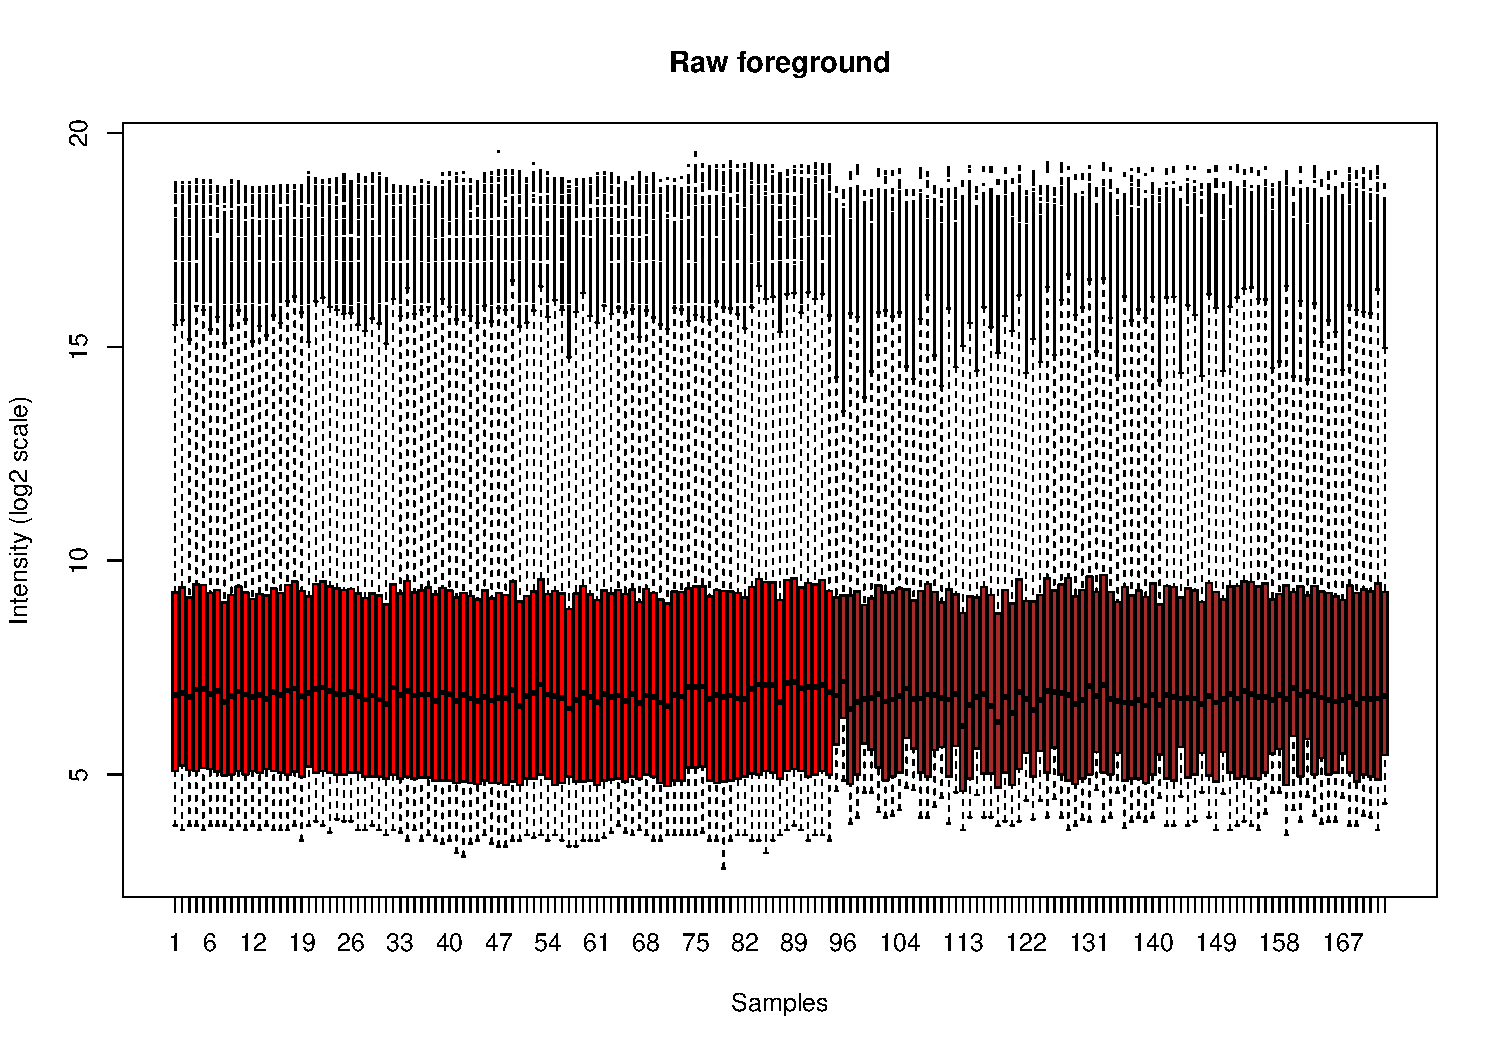
\includegraphics[width=1.0\textwidth,page=1]{mainmatter/figures/chapter_02/array_data_setup.array_intensity_boxplots.pdf}
    \caption{Raw foreground intensities for 173 \gls{HIRD} array samples. Colored by array processing batch.}
    \label{fig:hird_array_boxplots_raw}
\end{figure}

% Actually uses:
% The so-called glog2 (short for generalised logarithm) is a function that is like the logarithm (base 2) for large values (large compared to the amplitude of the background noise), but is less steep for smaller values.
VSN\autocite{huber2002VarianceStabilizationApplied} was used to perform background correction, between-array normalisation, and variance-stabilisation of intensity values, resulting in expression values on a $\log_2$ scale.

% 6.5.	Summarise probes (into loci): WGCNA::collapseRows(rowGroup=Ensembl ID, method="MaxMean", connectivityBasedCollapsing=FALSE)
% 6.5.1.	https://www.ncbi.nlm.nih.gov/pmc/articles/PMC3166942/
% 6.5.1.1.	“For example, we find that in most microarray experiments performed on brain tissue it is best to choose the probe with the maximum mean expression per gene, whereas when choosing a single gene to represent a co-expression module, the optimal collapsing method depends on the goal of the analysis.”
% 6.5.1.2.	“In the case of collapsing probes to their respective gene symbols, for example, we find that the 1.max strategy (implemented by setting method = "MaxMean" and connectivityBasedCollapsing = FALSE) produces the most robust results.”
% 6.5.1.3.	i.e. choose the probe with the highest mean of expression over the samples
Most genes are targetted by multiple array probes; 31208 probes were collapsed into 18216 Ensembl genes using by selecting the probe with the highest mean intensity for each gene (\texttt{WGCNA::collapseRows(method=MaxMean)}, recommended for probe to gene collapsing\autocite{miller2011StrategiesAggregatingGene}).
While it would be optimal to select a collapsing method to maximise the concordance between array and \gls{RNAseq} expression values, there were no samples assayed by both platforms in the \gls{HIRD} dataset.
The final normalised $\log_2$ intensity values for these 18216 genes over 173 samples is shown in \autoref{fig:hird_array_boxplots_MaxMean}.

\begin{figure}
    \centering
    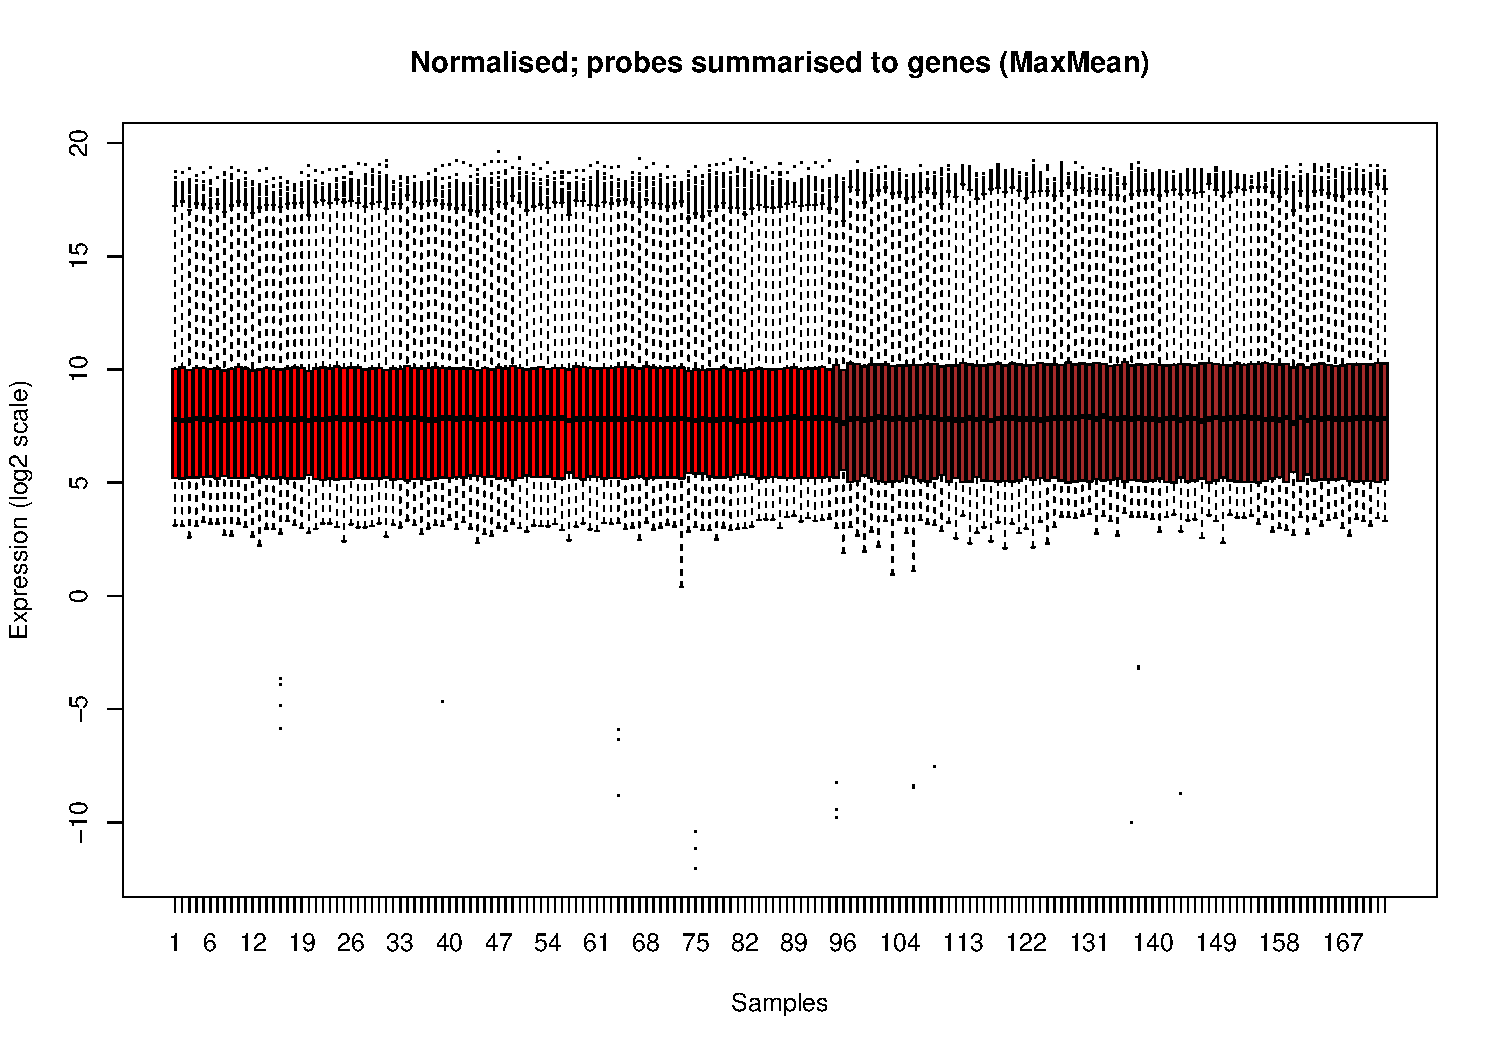
\includegraphics[width=1.0\textwidth]{mainmatter/figures/chapter_02/array_data_setup.array_intensity_boxplots.MaxMean.pdf}
    \caption{Array intensity estimates after VSN normalisation and collapsing of probes to genes. Colored by array processing batch.}
    \label{fig:hird_array_boxplots_MaxMean}
\end{figure}

\subsection{\Glsfmtlong{DGE}}

\gls{PCA} of the expression data reveals although samples separate by experimental timepoint along \gls{PC}3 (\autoref{fig:hird_expression_pcs}d), measurement platform is by far the largest source of variation.
Normalisation was also not able to completely remove the batch effect within the array data (\autoref{fig:hird_expression_pcs}a).
% Also see:
% Wang, C., Gong, B., Bushel, P. R., Thierry-Mieg, J., Thierry-Mieg, D., Xu, J., Fang, H., Hong, H., Shen, J., Su, Z., Meehan, J., Li, X., Yang, L., Li, H., Łabaj, P. P., Kreil, D. P., Megherbi, D., Gaj, S., Caiment, F., … Tong, W. (2014). The concordance between RNA-seq and microarray data depends on chemical treatment and transcript abundance. Nature Biotechnology, 32(9), 926–932. https://doi.org/10.1038/nbt.3001
%
% The CBM paper intro has a good summary too. https://www.ncbi.nlm.nih.gov/pmc/articles/PMC5510692/
The large platform effect likely stems from systematic technological differences in how each platform measures expression.
For example, arrays suffer from ratio compression due to cross-hybridisation\autocite{draghici2006ReliabilityReproducibilityIssues}.
\gls{RNAseq} has a higher dynamic range, resulting less bias at low expression levels, but estimates are more sensitive to changes in depth than array estimates are to changes in intensity \autocite{robinson2015NestedParallelExperiment}.
There are also differences in the statistical models behind expression quantification and normalisation, as described above\todo{cite relevant preprocessing sections}.

Despite the shortcomings of array data detailed above, the array dataset tends to contain individuals with more extreme antibody response phenotypes (\autoref{fig:hird_phenotypes_by_platform}), and hence the data should not be excluded.
Given the magnitude of the platform effect, I concluded that the appropriate approach should be a two-stage approach that integrates per-platform \gls{DGE} effect estimates while explicitly accounting for between-platform heterogeneity.

\begin{figure}
    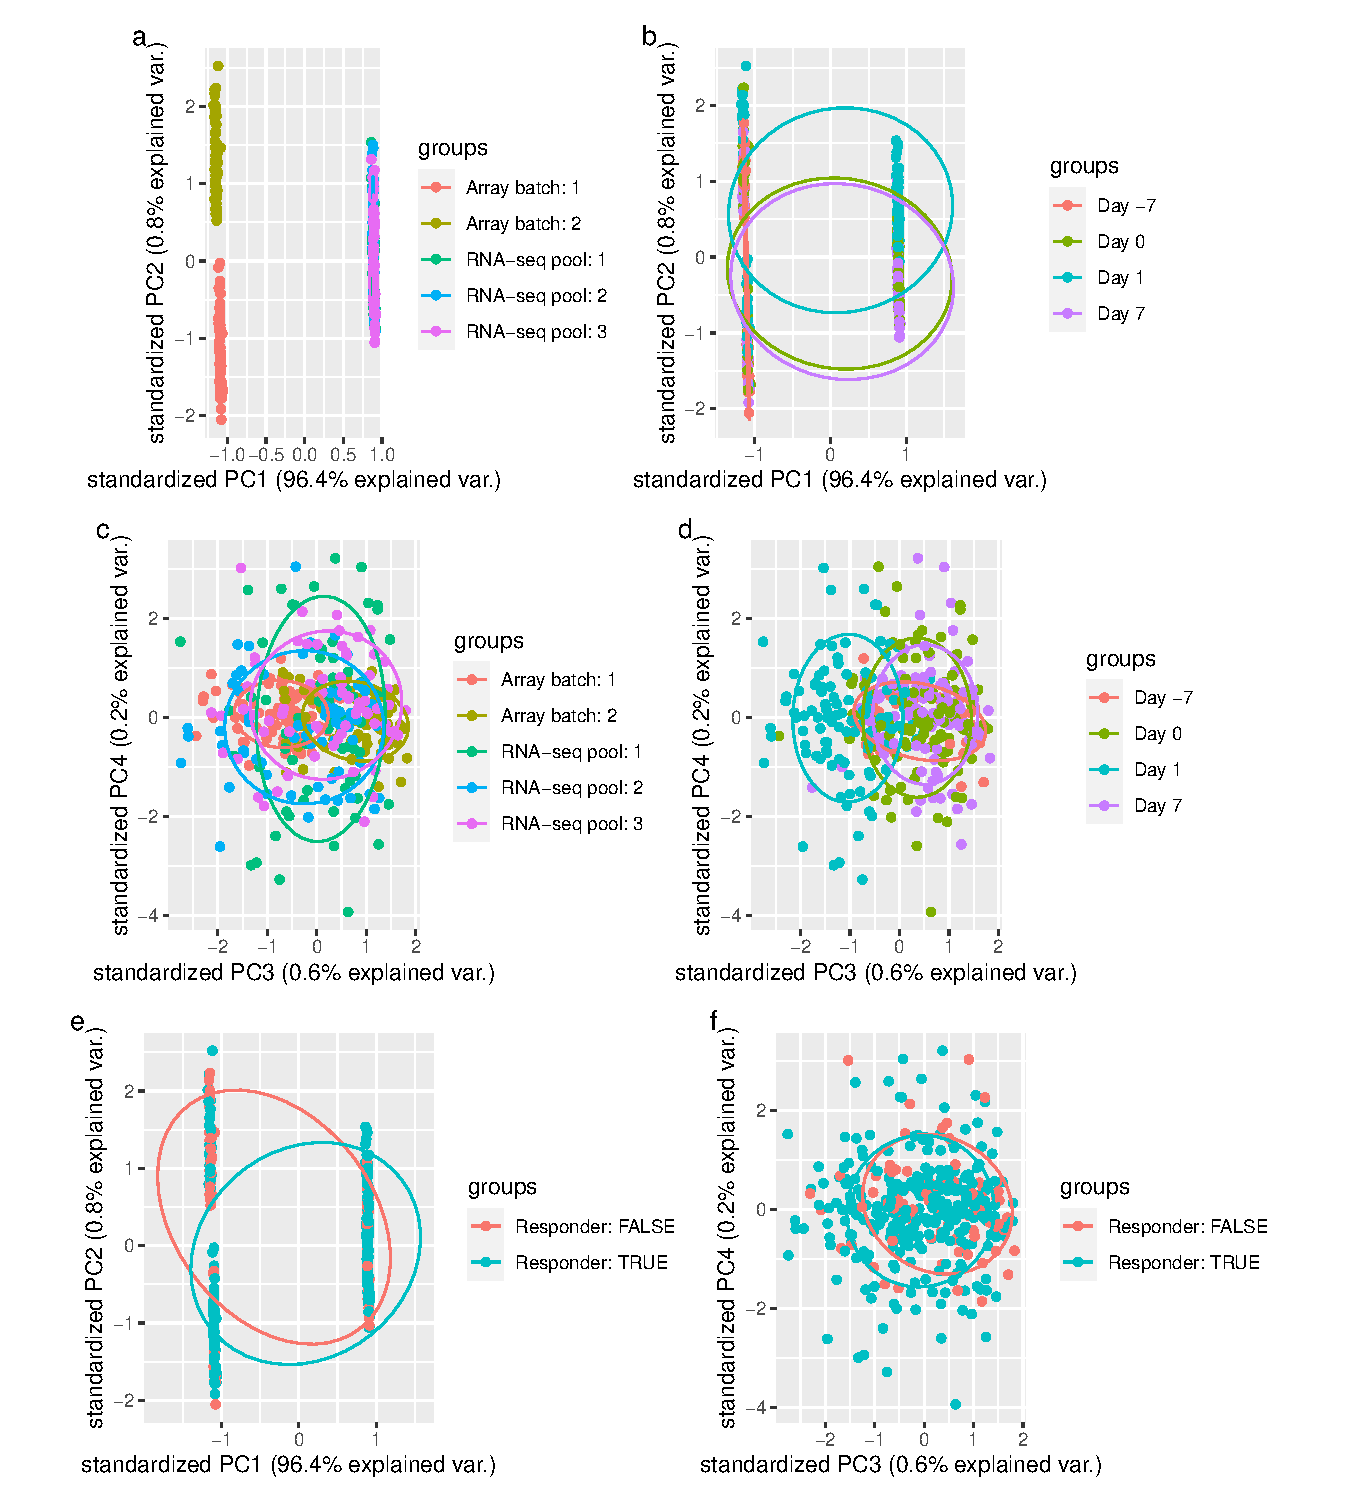
\includegraphics[width=1.0\textwidth,page=1]{mainmatter/figures/chapter_02/compare_phenotype_by_platform.E_pca.pdf}
    \caption{First four \glspl{PC} in the \gls{HIRD} expression data, colored by platform and batch (left), and timepoint (right).}
    \label{fig:hird_expression_pcs}
\end{figure}

% Also see: https://support.bioconductor.org/p/72815/
Regarding the batch effect within the array data, a popular adjustment method is ComBat\autocite{johnson2007AdjustingBatchEffects}, which estimates centering and scaling parameters by pooling information across all genes using empirical Bayes.
\todo{combat does have a pro in that it can do per gene scaling, that fixed fx won't do}
ComBat is the method used in \autocite{sobolev2016AdjuvantedInfluenzaH1N1Vaccination}.
In comparisons of microarray batch effect adjustment methods, ComBat performs favourably (vs. five other adjustment packages)\autocite{chen2011RemovingBatchEffects} or comparably (vs. batch as a fixed or random effect in the linear model)\autocite{espin-perez2018ComparisonStatisticalMethods}.
However, where batches are unbalanced in terms of sample size\autocite{zhang2018AlternativeEmpiricalBayes} or distribution of study groups that have an impact on expression\autocite{nygaard2015MethodsThatRemove}, ComBat can overcorrect batch differences or bias estimates of group differences respectively.
In our data, sample size and timepoint groups are fairly balanced between the two array batches, but the proportion of responders is not\autoref{tab:hird_batch_balance}, hence I elect not to use ComBat to pre-adjust the array expression data, and model the batches as fixed effects.
In practice, results from the \gls{DGE} analysis were not substantially affected by the choice of whether to use a ComBat pre-adjustment or a fixed effect.
\todo{this is not a very precise justification. actually, if I were to color R/NR in the PCA plot, R/NR doesn't really explain a lot of var in global gene expression. that's probably why the results don't change much.}
\todo{weaken this. combat is used multiple times in ch3}
\todo{be more specific about how combat works i.e. estimates factors per gene per batch?}

\begin{table}[] 
 \centering 
 \caption[\captionshort{Distribution of \gls{HIRD} samples among timepoint and responder groups in the array batches and \gls{RNAseq} pools.}]{\textbf{Distribution of \gls{HIRD} samples among timepoint and responder groups in the array batches and \gls{RNAseq} pools.} Values are count and percentage for categorical variables; mean and standard deviation for continuous variables.}\label{tab:hird_batch_balance}
 \begin{tabular}{ l c c c c c c }
 \toprule
  &   &  \multicolumn{ 5 }{c}{ Array batch/\gls{RNAseq} pool }\\ 
  & Total & Array 1 & Array 2 & \gls{RNAseq} 1 & \gls{RNAseq} 2 & \gls{RNAseq} 3\\ 
  & n = 374 & n = 87 & n = 79 & n = 70 & n = 69 & n = 69 \\ 
  \midrule
 Day &   &   &   &   &   &  \\ 
 \hspace{6pt}    -7 & 40 (10.7\%) & 20 (23\%) & 20 (25.3\%) & 0 (0\%) & 0 (0\%) & 0 (0\%)\\ 
 \hspace{6pt}    0 & 114 (30.5\%) & 24 (27.6\%) & 20 (25.3\%) & 24 (34.3\%) & 23 (33.3\%) & 23 (33.3\%)\\ 
 \hspace{6pt}    1 & 109 (29.1\%) & 21 (24.1\%) & 20 (25.3\%) & 22 (31.4\%) & 23 (33.3\%) & 23 (33.3\%)\\ 
 \hspace{6pt}    7 & 111 (29.7\%) & 22 (25.3\%) & 19 (24.1\%) & 24 (34.3\%) & 23 (33.3\%) & 23 (33.3\%)\\ 
 Responder &   &   &   &   &   &  \\ 
 \hspace{6pt}    FALSE & 80 (21.4\%) & 12 (13.8\%) & 36 (45.6\%) & 11 (15.7\%) & 9 (13\%) & 12 (17.4\%)\\ 
 \hspace{6pt}    TRUE & 294 (78.6\%) & 75 (86.2\%) & 43 (54.4\%) & 59 (84.3\%) & 60 (87\%) & 57 (82.6\%)\\ 
 TRI &   &   &   &   &   &  \\ 
 \hspace{6pt}   & -0.1 (1.0) & -0.1 (1.0) & -0.4 (1.4) & 0.1 (0.6) & -0.0 (0.8) & 0.2 (0.6)\\ 
 \bottomrule
 
 \end{tabular}
 \end{table}


\subsubsection{Per-platform \glsfmtlong{DGE} model}

% Also used arrayWeights as precision weight inputs to lmFit
% See: https://bmcbioinformatics.biomedcentral.com/articles/10.1186/1471-2105-7-261#Bib1
% The method successfully assigns lower weights to less reproducible arrays from different experiments. Down-weighting the observations from suspect arrays increases the power to detect differential expression.
For the array data, as \autocite{sobolev2016AdjuvantedInfluenzaH1N1Vaccination} demonstrated no significant global differences in expression between day -7 and day 0, I likewise merge these two timepoints into a single \enquote{day 0} baseline timepoint in the following \gls{DGE} models.

% 5.6.	Between-sample normalization of library size: Trimmed mean of M-values (TMM)
% Selecting between-sample RNA-Seq normalization methods from the perspective of their assumptions https://www.ncbi.nlm.nih.gov/pmc/articles/PMC6171491/
% 5.6.1.	edgeR::calcNormFactors generates norm.factors for each sample
For the \gls{RNAseq} data, between-sample normalisation was performed using the \gls{TMM} method\autocite{evans2018SelectingBetweensampleRNASeq} from edgeR\autocite{robinson2010EdgeRBioconductorPackage}; 
then variance-stabilisation was performed using voom\autocite{law2014VoomPrecisionWeights}, resulting in expression values with units of $\log_2{\text{\gls{CPM}}}$.
\todo{this is DGE specific normalisation, which is why it goes here, not in the preprocessing section}

% 7.	Differential expression (limma)
% 7.2.	Create contrasts
% 7.3.	Estimate within-block correlation (duplicateCorrelation), using patients as blocks
% 7.4.	Array data only: Compute sample quality weights for each array (arrayWeightsSimple(v, design=mod1))
% 7.5.	RNA-seq data only: Correct for mean-variance trend (voom)
% 7.5.1.	http://web.mit.edu/~r/current/arch/i386_linux26/lib/R/library/limma/html/voom.html
% 7.5.1.1.	“voom is an acronym for mean-variance modelling at the observational level. The key concern is to estimate the mean-variance relationship in the data, then use this to compute appropriate weights for each observation. Count data almost show non-trivial mean-variance relationships. Raw counts show increasing variance with increasing count size, while log-counts typically show a decreasing mean-variance trend. This function estimates the mean-variance trend for log-counts, then assigns a weight to each observation based on its predicted variance. The weights are then used in the linear modelling process to adjust for heteroscedasticity.”
% 7.5.1.2.	“voom performs the following specific calculations. First, the counts are converted to logCPM values, adding 0.5 to all the counts to avoid taking the logarithm of zero. The matrix of logCPM values is then optionally normalized. The lmFit function is used to fit row-wise linear models. The lowess function is then used to fit a trend to the square-root-standard-deviations as a function of average logCPM. The trend line is then used to predict the variance of each logCPM value as a function of its fitted value, and the inverse variances become the estimated precision weights.”
% 7.6.	(lmFit)
% 7.7.	(contrasts.fit)
% 7.8.	(eBayes/treat)
% 7.8.1.1.1.	https://rdrr.io/bioc/limma/man/ebayes.html
% 7.8.1.1.1.1.	When lfc=0, treat is identical to eBayes, except that F-statistics and B-statistics are not computed.
% 7.8.1.1.2.	https://academic.oup.com/bioinformatics/article/25/6/765/251641 The TREAT fold-change threshold should be set to a low value below which no fold-change is likely to be of genuine interest. Researchers should be mindful that genes will need to exceed this threshold by some way, depending on the data, before being declared statistically significant. Our experience suggests a minimal value, such as a 10% fold-change, corresponding to τ=log2(1.1)=0.13 on the log2-scale. It would be better to interpret the threshold as ‘the fold-change below which we are definitely not interested in the gene’ rather than ‘the fold-change above which we are interested in the gene’.
% 7.9.	(decideTests)
Linear models were fit using limma\autocite{ritchie2015LimmaPowersDifferential}, which is computationally fast, and performs well for sufficiently large ($n \ge 3$ per group) sample sizes\autocite{soneson2013ComparisonMethodsDifferential}.
For each gene, I fit a model (model 1) with expression as the response variable; with timepoint (baseline, day 1, day 7), \gls{TRI}, batch, sex, age, and the first 4 genotype \glspl{PC} as fixed-effect predictors; and individual as a random-effect predictor.
\todo{link to papers justifying sex, age, ancestry as significant effects on immune gene expression}
Within-individual correlations for the random effect were estimated using limma::duplicateCorrelation.
A second model (model 2) was also fit, including 3 additional terms for the interactions between each timepoint and \gls{TRI}.
% https://support.bioconductor.org/p/70175/
% es <- fit2$coefficients
% es_se <- sqrt(fit2$s2.post) * fit2$stdev.unscaled
From model 1, I defined contrasts for day 1 vs. baseline, day 7 vs. baseline, day 7 vs. day 1, \gls{TRI}, sex, and age.
From model 2, I defined contrasts for the \gls{TRI} specifically at each of the three timepoints.
Corresponding coefficients and standard errors for the contrasts were extracted from the linear models, which represent effect size in units of $\log_2$ expression fold change per unit change in predictor value.

\subsubsection{Choice of \glsfmtlong{DGE} meta-analysis method}
\label{subsubsec:hird_dge_meta_methodChoice}

In the section \todo{add section labels}, I concluded that a two-stage meta-analysis approach would be appropriate.
This meta-analysis is restricted to 13593 genes assayed by both the array and \gls{RNAseq} platforms.
% While there is abundant literature on single-plaform (e.g. \autocite{tseng2012ComprehensiveLiteratureReview}) methods [...]
%
% Examples from literature
%
% random effects:
%
% https://academic.oup.com/nar/article/45/17/9860/4084660#106485896
% - for example of REM of 24 array datasets
%
% Sweeney, T. E., Haynes, W. A., Vallania, F., Ioannidis, J. P., & Khatri, P. (2017). Methods to increase reproducibility in differential gene expression via meta-analysis. Nucleic Acids Research, 45(1), e1–e1. https://doi.org/10.1093/nar/gkw797
% - DGE random effects models should be possible with around 6-7 studies.
%
% SVA:
% Comparative RNA-Seq and Microarray Analysis of Gene Expression Changes in B-Cell Lymphomas of Canis familiaris
% https://www.ncbi.nlm.nih.gov/pmc/articles/PMC3617154/
% - applying SVA to our data revealed a strong correlation with known technical biases associated with RNA-Seq [26]–[28], [51] and removing the associated variation from the RNA-Seq samples resulted in the two technologies pairing by individual sample.
% - First, we have not attempted to capture differences in dynamic range between RNA-Seq and microarray. It is reasonable to expect that the larger dynamic range of RNA-Seq will result in larger variation. We found latent variation to be highly associated with GC content but, in contrast, found no clear evidence of an association pointing to nonlinear response in the microarrays. Second, the model underlying SVA does not explicitly capture different latent variables for the different technologies.
%
% MetaVolcano:
% The MetaVolcanoR R package combines differential gene expression results. It implements three strategies to summarize gene expression activities from different studies. i) Random Effects Model (REM) approach. ii) a vote-counting approach, and iii) a p-value combining-approach.
% - doesn't solve our small k problem
%
% CorMotif:
% https://academic.oup.com/biostatistics/article/16/1/31/259492
% - In contrast, a model that naively enumerates and analyzes all possible differential patterns across studies can deal with study-specificity and allow information pooling, but the complexity of its parameter space grows exponentially as the number of studies increases.
% - Here, we propose a correlation motif approach to address this dilemma. This approach searches for a small number of latent probability vectors called correlation motifs to capture the major correlation patterns among multiple studies.
% - First applies limma (Smyth, 2004) to each study separately. CorMotif is made for microarray data since it was motivated by the microarray analysis in the Sleep for Health in Hospital Programme (SHH) study. However, the idea behind CorMotif is general, and it should be straightforward to develop a similar framework for RNA-seq data.
% - designed for large k, seems similar to mashr
%
% CBM (“Cross-platform Bayesian Model”):
% - In this article, we propose a Bayesian hierarchical model to jointly integrate microarray and RNA-seq studies.
% - Since systematic fold change differences across RNA-seq and microarray for detecting differentially expressed genes have been previously reported, we replicated this finding in several real datasets and showed that incorporation of a normalization procedure to account for the bias improves the detection accuracy and power.
% - Cannot acually use CBM, as it operates on expressions, with a binary case vs control, so no covariates
%
% RankProd:
% - The Bioconductor package RankProd provides a new and intuitive tool for this purpose in detecting differentially expressed genes under two experimental conditions.
%
% Mayday seasight:
% - Uses a rank product model internally

Two popular frameworks for effect size meta-analysis are fixed-effect and random-effects\autocite{cohn2003HowMetaanalysisIncreases,borenstein2010BasicIntroductionFixedeffect}.
Given k studies, the fixed-effect model assumes a common population effect size shared across all studies, with observed variation explained only by sampling error.
The random-effects model assumes the k study-specific effect sizes are drawn from some distribution with variance $\tau^2$ (\gls{SD} $\tau$), representing an additional source of variation termed the between-studies heterogeneity, reducing to the fixed-effect model when $\tau=0$.
In the \gls{HIRD} data, there are $k=2$ 'studies' (array and \gls{RNAseq}), where the platform differences described in section\todo{add label} contribute to considerable between-studies heterogeneity.
The assumption of $\tau=0$ is unrealistic, hence a random-effects model is more appropriate.
\todo{make all the notation in this section consistent with, and add the equation 2.1. The normal-normal hierarchical model, \autocite{rover2017BayesianRandomeffectsMetaanalysis}}

Unfortunately, there is no optimal solution for directly estimating $\tau$ in random-effects meta-analyses with small k\autocite{bender2018MethodsEvidenceSynthesis}, in the case of $k=2$ especially\autocite{gonnermann2015NoSolutionCombining}.
Many estimators are available\autocite{veroniki2016MethodsEstimateBetweenstudy}, but lack of information with small k causes estimation to be imprecise, and often results in boundary values of $\tau = 0$ that are incompatible with the assumed positive heterogeneity\autocite{chung2013NondegeneratePenalizedLikelihood,friede2017MetaanalysisFewSmall}.
In such circumstances, the most sensible choice may be to incorporate prior information about model hyperparameters in a Bayesian random-effects framework\autocite{chung2013NondegeneratePenalizedLikelihood,veroniki2016MethodsEstimateBetweenstudy,friede2017MetaanalysisFewSmall,seide2019LikelihoodbasedRandomeffectsMetaanalysis}.
For this study, I use the implementation in bayesmeta \autocite{rover2017BayesianRandomeffectsMetaanalysis}, which requires priors for both effect size and between-studies heterogeneity.

\subsubsection{Prior for between-studies heterogeneity}

The choice of prior for between-studies heterogeneity is influential when k is small\autocite{seide2019LikelihoodbasedRandomeffectsMetaanalysis}.
\textcite{gelman2006PriorDistributionsVariance} considers the case of $k=3$, showing that a flat prior places too much weight on implausibly large estimates of $\tau$, and recommends a weakly informative prior that acts to regularise the posterior distribution.
% Gelman 
% - weak as in deliberately weaker than known knowledge, just serves to constrain
% - cauchy for the gentle slope in tails
% - also warns against inverse-gamma(e, e), as it can influence the posterior mean; it is not at all non-informative.
%
% Similarly, \autocite{friede2017MetaanalysisFewSmall} consider half-normals.
%
% More recent recommendations:
% \footnote{Documentation for Stan: \url{https://github.com/stan-dev/stan/wiki/Prior-Choice-Recommendations}.}
% - Gelman 2006 recommendations can actually be too weak for scale
% - Recommends Chung gamma(2, 1/A)
% - With full Bayes the boundary shouldn't be a problem (as long as you have any proper prior).
% - But with modal estimation, the estimate can be on the boundary, which can create problems in posterior predictions. For example, consider a varying-intercept varying-slope multilevel model which has an intercept and slope for each group. Suppose you fit marginal maximum likelihood and get a modal estimate of 1 for the group-level correlation. Then in your predictions the intercept and slope will be perfectly correlated, which in general will be unrealistic.
% Chung, Y., Rabe-Hesketh, S., Dorie, V., Gelman, A., & Liu, J. (2013). A Nondegenerate Penalized Likelihood Estimator for Variance Parameters in Multilevel Models. Psychometrika, 78(4), 685–709. https://doi.org/10.1007/s11336-013-9328-2
Since I assumed zero estimates for $\tau$ are unrealistic, I use a weakly-informative gamma prior recommended by \autocite{chung2013NondegeneratePenalizedLikelihood}, which has zero density at $\tau = 0$, increasing gently as $\tau$ increases.
This constrains $\tau$ to be positive, but still permits estimates close to zero if the data support it.
This is in constrast to priors used in other studies from the log-normal (e.g. \autocite{pullenayegum2011InformedReferencePrior,turner2015PredictiveDistributionsBetweenstudy}) or inverse-gamma (e.g. \autocite{higgins1996BorrowingStrengthExternal}) families that have derivatives or zero close to zero, thus ruling out small values of $\tau$ no matter what the data suggest; and in contrast to half-t family priors (e.g. \autocite{gelman2006PriorDistributionsVariance,seide2019LikelihoodbasedRandomeffectsMetaanalysis}), which have their mode at zero, and do not rule out $\tau=0$.

% rma.uni function
% By default, the starting value is set equal to the value of the Hedges (HE) estimator and the algorithm terminates when the change in the estimated value of \tau2 is smaller than 10^-5 from one iteration to the next.
To estimate the appropriate shape and scale parameters for the gamma empirically, a frequentist random-effects model using the \gls{REML} estimator for $\tau$ (recommended for continuous effects\autocite{veroniki2016MethodsEstimateBetweenstudy}) was first for each gene using \texttt{metafor::rma}.
Genes with small estimates of $\tau < 0.01$ were excluded, and a gamma distribution was fit to the remaining estimates using \texttt{fitdistrplus}.

\subsubsection{Prior for effect size}

While the choice of prior on $\tau$ is influential when k is small, there is usually enough data to estimate the effect size $\mu$ such that any reasonable non-informative prior can be used \autocite{gelman2006PriorDistributionsVariance,friede2017MetaanalysisFewSmall}.
\todo{why is this? is it having well powered studies? gelman is vague}
\texttt{bayesmeta} implements both flat and normal priors for $\mu$.
%
% https://github.com/stan-dev/stan/wiki/Prior-Choice-Recommendations
% For example, it is common to expect realistic effect sizes to be of order of magnitude 0.1 on a standardized scale (for example, an educational innovation that might improve test scores by 0.1 standard deviations). In that case, a prior of N(0,1) could be considered very strong, in that it puts most of its mass on parameter values that are unrealistically large in absolute value. When we say this prior is "weakly informative," what we mean is that, if there's a reasonably large amount of data, the likelihood will dominate, and the prior will not be important. If the data are weak, though, this "weakly informative prior" will strongly influence the posterior inference. The phrase "weakly informative" is implicitly in comparison to a default flat prior.
% Weakly informative prior should contain enough information to regularize: the idea is that the prior rules out unreasonable parameter values but is not so strong as to rule out values that might make sense
% Weakly informative rather than fully informative: the idea is that the loss in precision by making the prior a bit too weak (compared to the true population distribution of parameters or the current expert state of knowledge) is less serious than the gain in robustness by including parts of parameter space that might be relevant. It's been hard for us to formalize this idea.
% One principle: write down what you think the prior should be, then spread it out. The idea is that the cost of setting the prior too narrow is more severe than the cost of setting it too wide. I've been having trouble formalizing this idea.
% Don't use uniform priors, or hard constraints more generally, unless the bounds
% represent true constraints (such as scale parameters being restricted to be
% positive, or correlations restricted to being between -1 and 1).
Assuming that most genes are not differentially expressed with effect sizes distributed randomly around zero, I selected a normal prior with $N(\mu=0, \sigma^2)$, over a flat prior. As in the section above, to determine an appropriate scale, a normal distribution with mean $\mu = 0$ was fit to the distribution of effect sizes from the gene-wise frequentist models to empirically estimate $\sigma$.

% Another Cauchy example:
% Gelman, A., Jakulin, A., Pittau, M. G., & Su, Y.-S. (2008). A weakly informative default prior distribution for logistic and other regression models. The Annals of Applied Statistics, 2(4), 1360–1383. https://doi.org/10.1214/08-AOAS191
% - Cauchy 2.5
Heavy-tailed Cauchy priors have been proposed for effect size distributions in \gls{DGE} experiments to avoid over-shrinkage of true large effects in the tails\autocite{zhu2019HeavytailedPriorDistributions}.
Since \texttt{bayesmeta} does not implement a Cauchy prior, to avoid over-shrinkage, I flatten the normal prior considerably by scaling up the variance to $N(0, 100\sigma^2)$.
This is equivalent to assuming placing a 95\% prior probability that effects are less extreme than approximately $20\sigma$.\todo{the derivation here is qnorm(0.975, mean=0, sd=1*10) = 1*19.59964, bit iffy, double check this is correct}

\subsubsection{Evaluation of priors}

An example of the empirically estimated hyperparameters for the priors for the day 1 vs. baseline contrast are shown in \autoref{fig:hird_dgeMeta_priors_tau} (for $\tau$) and \autoref{fig:hird_dgeMeta_priors_mu} (for $\mu$).
For $\tau$, the final prior used was $\text{Gamma}(\text{shape}=1.5693, \text{scale}=0.0641)$.
This is comparable to \autocite{chung2013NondegeneratePenalizedLikelihood}'s default recommendation of a $\text{Gamma}(\text{shape}=2, \text{scale}=\lambda)$ prior where $\lambda$ is small.
\todo{could also include a table of all sets of parameters here?}
For $\mu$, the final prior used was $N(0, (0.3240*10)^2)$.
The tails of the non-scaled normal fit (black) are light compared to the Cauchy fit (red), which may lead to over-shrinkage, especially since there are many genes with high positive fold changes for the day 1 vs. baseline effect.

\begin{figure}
    \includegraphics[width=1.0\textwidth,page=2]{mainmatter/figures/chapter_02/meta.bayesmeta.priors.coefName_d1.vs.d0.pdf}
    \caption{Gamma prior for $\tau$ used for \texttt{bayesmeta} (blue), compared to the empirical distribution of per-gene frequentist \texttt{metafor::rma} estimates for $\tau$, for the day 1 vs. baseline effect (small estimates of $\tau < 0.01$ excluded). Empirical log-normal fit also shown (red).}
    \label{fig:hird_dgeMeta_priors_tau}
\end{figure}

\begin{figure}
    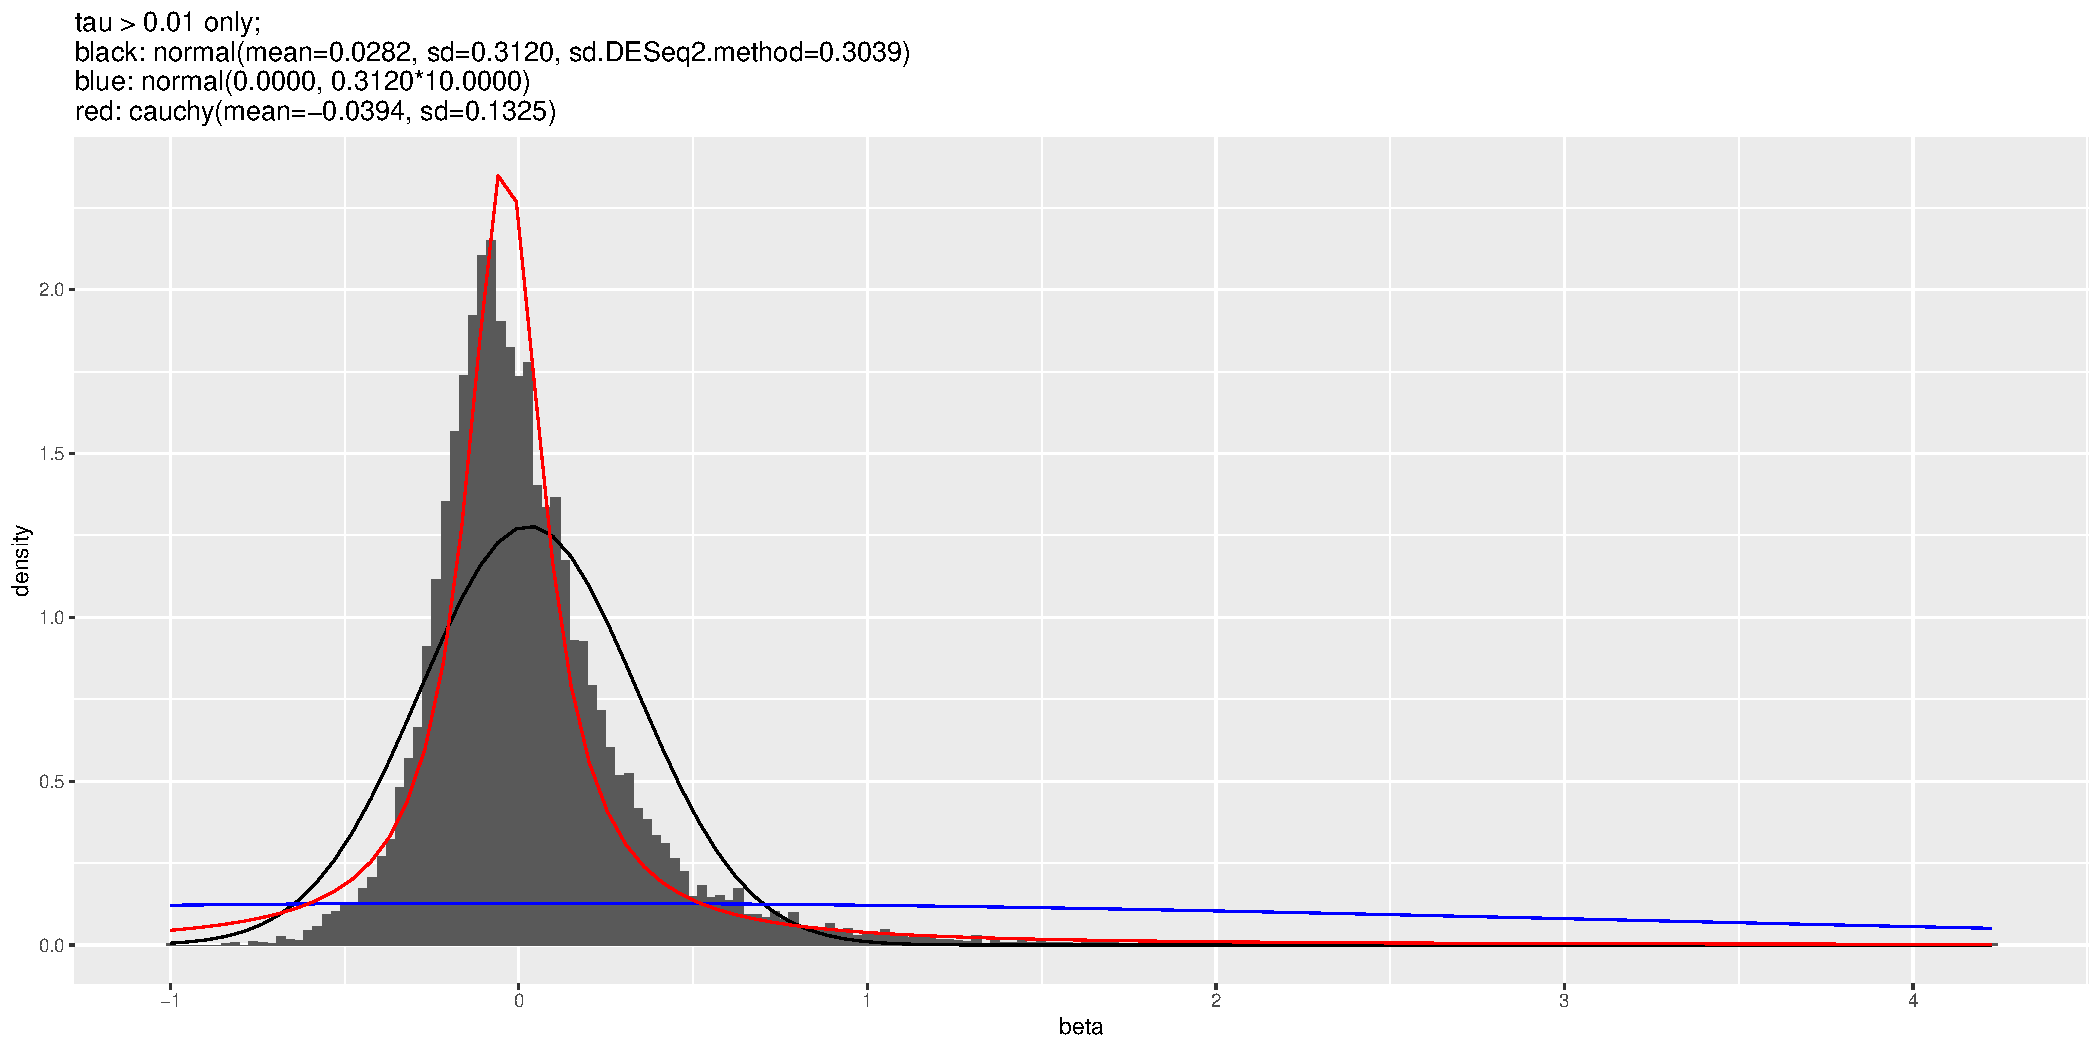
\includegraphics[width=1.0\textwidth,page=1]{mainmatter/figures/chapter_02/meta.bayesmeta.priors.coefName_d1.vs.d0.pdf}
    \caption{Normal prior for $\mu$ used for \texttt{bayesmeta} (blue), compared to the empirical distribution of per-gene frequentist \texttt{metafor::rma} estimates for $\tau$, for the day 1 vs. baseline effect. The non-scaled normal fit is shown (black), as well as a Cauchy fit (red).}
    \label{fig:hird_dgeMeta_priors_mu}
\end{figure}

\subsubsection{Multiple testing correction}

For the frequentist random-effects meta-analysis, nominal gene-wise p values are converted to \gls{FDR} estimates using the \gls{BH} procedure (\texttt{p.adjust} in R).
For the Bayesian random-effects meta-analysis, posterior effect sizes and standard errors are supplied to \texttt{ashr}, which estimates the \glspl{lfsr}, which are analogous to \gls{FDR}, but quantifies the probability of calling the wrong sign for an effect rather than than the confidence of a non-zero effect\autocite{stephens2016FalseDiscoveryRates}.
\todo{add comment on symmetry}
%
% bayesmeta
% Posterior predictive checks are implemented in the pppvalue() to generate pvalues by MCMC.
% Do not confuse with ma05$pposterior(mu=0), which is evaluation of the posterior distribution at a particular value.

\subsection{Gene set enrichment analysis using \glsfmtlongpl{BTM}}

Gene set enrichment analyses were conducted using \texttt{tmod::tmodCERNOtest}\autocite{weiner3rd2016TmodPackageGeneral}, which assesses the enrichment of small ranks within specific sets of genes compared to all genes, when the genes are ranked by some metric---here I used effect sizes from \texttt{bayesmeta}.
The gene sets used were \glspl{BTM} from\autocite{li2013MolecularSignaturesAntibody}, which are annotated sets of coexpressed genes mined from publicly available human blood transcriptomic data, and provide sets tailored for enrichment analyses in blood cells.

\section{Results}

\subsection{Extensive global changes in expression after vaccination}

To gain an overview of how the transcriptome changes after vaccination, linear models were fit to identify genes differentially expressed at day 1 or day 7 compared to baseline (day -7 and day 0) in the \gls{HIRD} array and \gls{RNAseq} expression data, accounting for covariates such as batch effects, sex, age, \gls{TRI}, and ancestry.
At 13593 genes with expression measured by both platforms, models were fit within each platform, then effect sizes were combined using Bayesian random-effects meta-analysis.

At a $\text{\gls{lfsr}} < 0.05$ and absolute $\text{\gls{FC}} > 1.5$ cutoff, 857/13593 genes were differentially expressed between any pair of timepoints, with their expression clustering into three main clusters (\autoref{fig:hird_dge_heatmap}).
% 692 genes with high expression at day 1, 94 genes with high expression at day 7, and 59 genes with low expression at day 1
 
\begin{figure}
    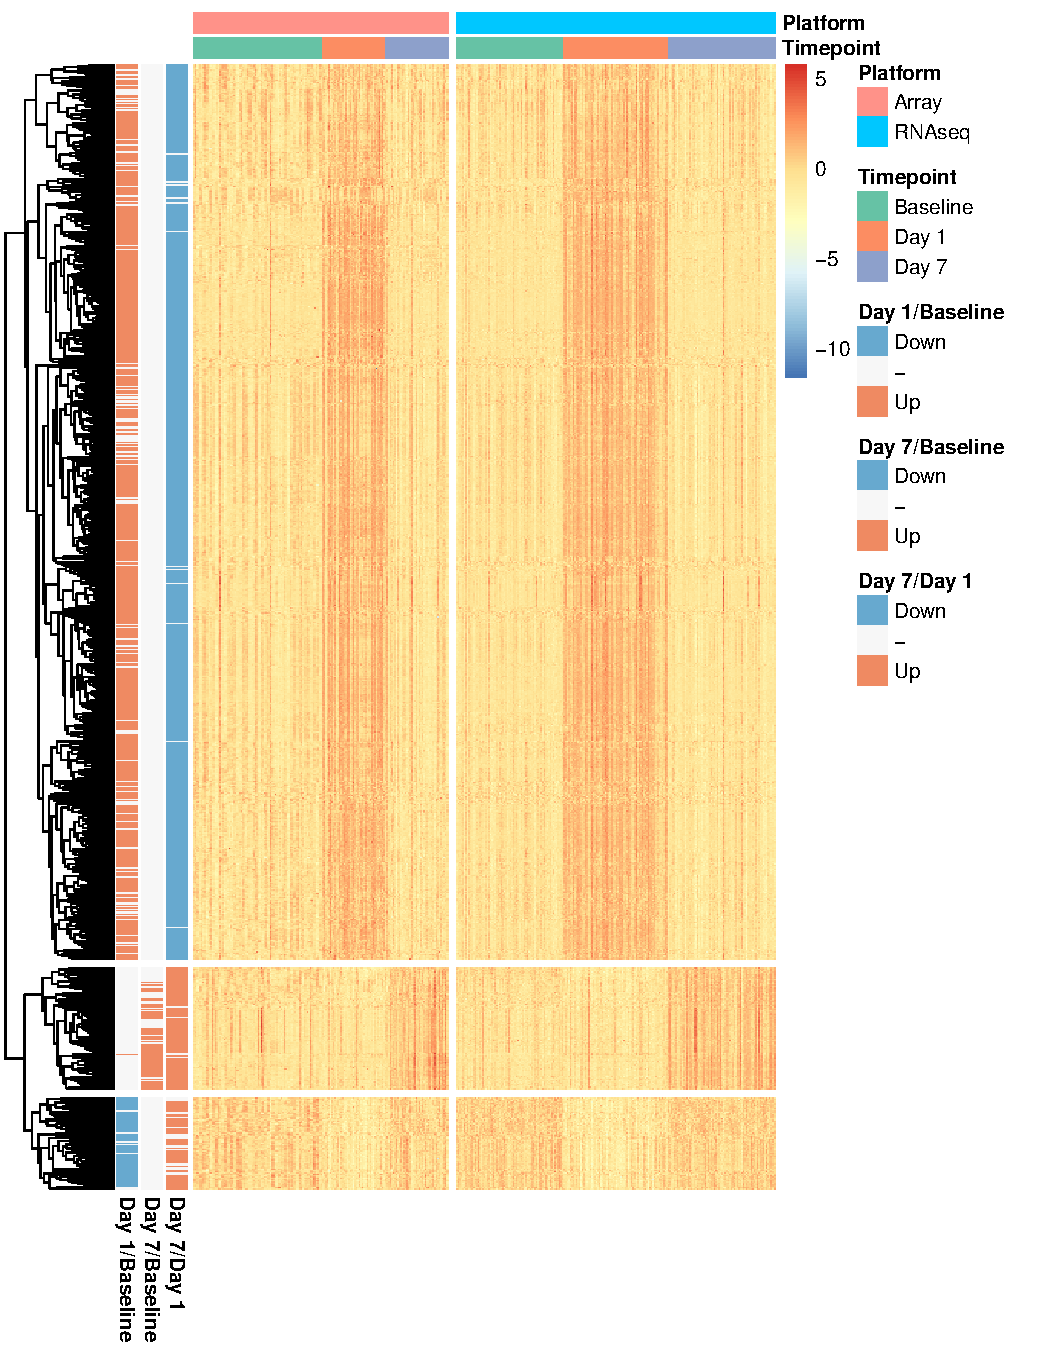
\includegraphics[width=1.0\textwidth]{mainmatter/figures/chapter_02/plot_dge_eqtl.heatmap_dge.pdf}
    \caption{Normalised gene expression for genes differentially expressed between any pair of timepoints ($\text{lfsr} < 0.05$, $\text{absolute fold change} > 1.5$) across \gls{HIRD} samples, clustered by gene (Manhattan distance metric).}
    \label{fig:hird_dge_heatmap}
\end{figure}

\subsection{Innate immune response at day 1 post-vaccination}

Consistent with global expression at day 1 being markedly different from expression at other timepoints (\autoref{fig:hird_expression_pcs}), the highest numbers of differentially expressed genes are observed at day 1, with 644 genes differentially expressed vs. baseline.
The majority of these (580/644) were upregulated.
The gene with the highest \gls{FC} increase at day 1 compared to baseline was \gene{ANKRD22} ($\log_2\text{\gls{FC}} = \num{4.489150}$), an interferon-induced gene in monocytes and \glspl{DC} involved in antiviral innate immune pathways\autocite{bin2016AnkyrinRepeatDomain}.
Other key genes in the interferon signalling pathway\autocite{schneider2014InterferonStimulatedGenesComplex} such as \gene{STAT1} ($\log_2\text{\gls{FC}} = 2.1693060$), \gene{STAT2}   ($\log_2\text{\gls{FC}} = 0.9489341$), and \gene{IRF9} ($\log_2\text{\gls{FC}} = 0.8153674$) are also upregulated at day 1.
Gene set enrichment analysis using \texttt{tmod} revealed that genes with the high \gls{FC} increases at day 1 were enriched in modules associated with activated \glspl{DC}, monocytes, toll-like receptor and inflammatory signalling (\autoref{fig:hird_tmodDotPlot_timepoint}), confirming that day 1 responses are dominated by signatures of innate immunity.
\todo{can also add MSigDB hallmark sets, which include interferon sets; and of course gene ontology sets}
64 genes were downregulated at day 1, enriched in modules associated with T cells and \gls{NK} cells, with the largest absolute fold change observed for \gene{FGFBP2} ($\log_2\text{\gls{FC}} = -0.9141547$).
\todo{not sure of interpretation at FGFBP2, it is indeed highly expressed in NKs through \url{https://dice-database.org/genes/FGFBP2}}
For both up and downregulated genes, there was a tendency to return to baseline expression levels by day 7.
\todo{any point in a table of e.g. top 20 DE genes, or is the gene set analysis already enough?}

\begin{figure}
    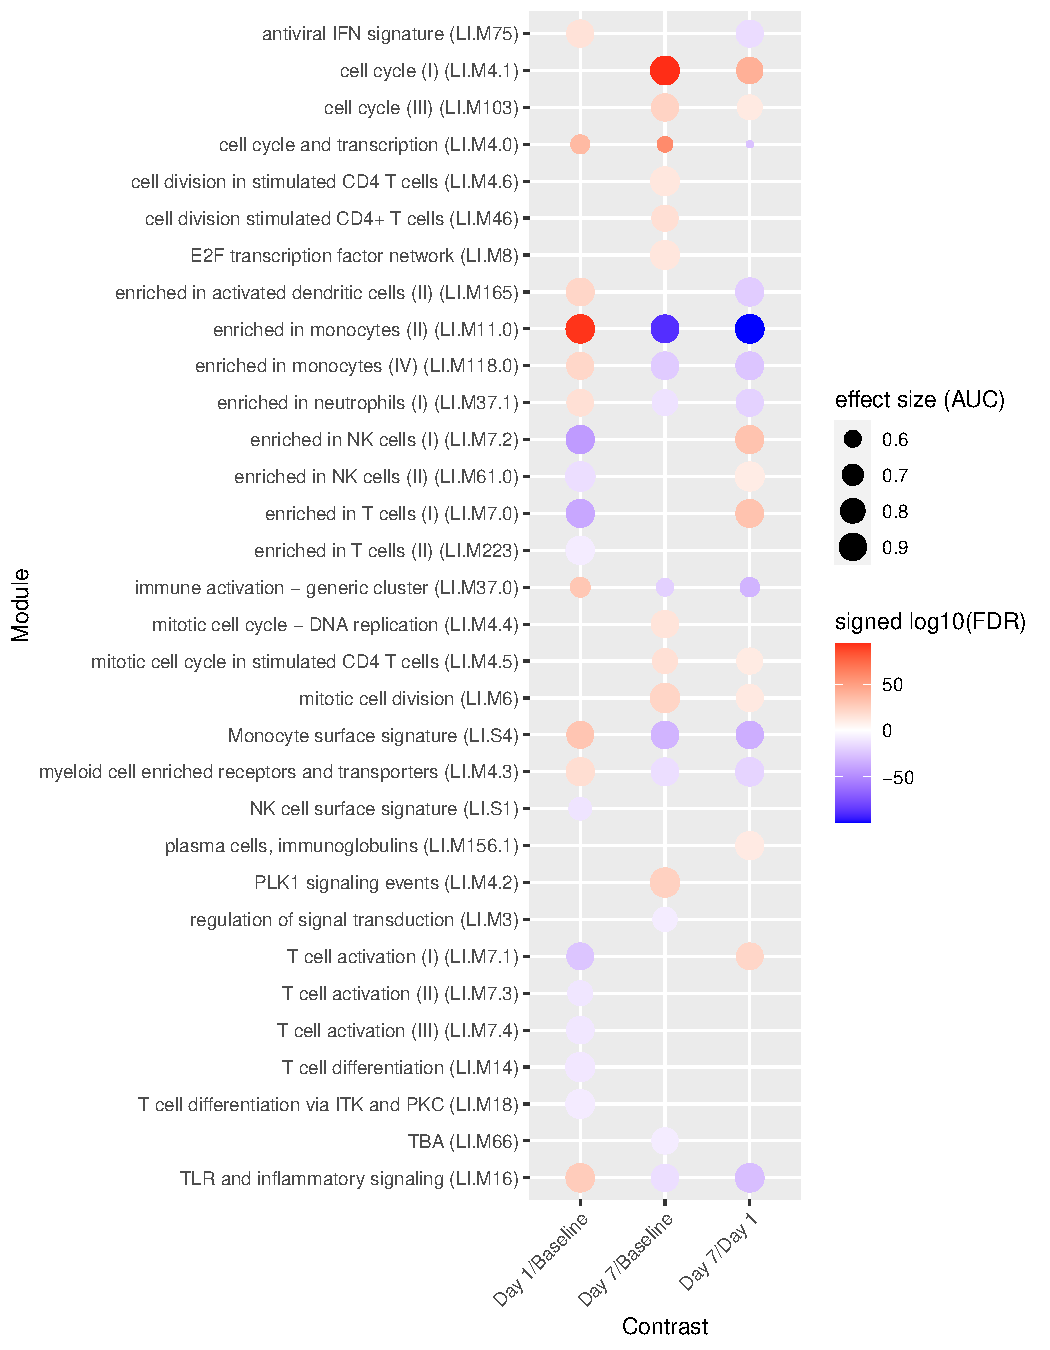
\includegraphics[width=1.0\textwidth]{mainmatter/figures/chapter_02/compare_dge_eqtl.tmodDotPlot.DGE.timepoint.pdf}
    \caption{Transcriptomic modules significantly up or downregulated post-vaccination. Size of circle indicates effect size. Color of circle indicates significance and direction of effect (red = upregulation, blue = downregulation).}
    \label{fig:hird_tmodDotPlot_timepoint}
\end{figure}
\todo{change x axis labels to baseline, specify top 10 procedure in figure caption}

\subsection{Adaptive immune response at day 7 post-vaccination}

59 genes were differentially expressed at day 7 vs. baseline, with expression fold changes more modest than those at day 1.
The genes with the highest upregulation were the B cell-associated genes \gene{TNFRSF17} ($\log_2\text{\gls{FC}} = 1.7538617$) and \gene{MZB1} ($\log_2\text{\gls{FC}} = 1.7369668$).
Plasma cell-specific genes including \gene{SDC1} (encodes CD138 \url{https://www.ncbi.nlm.nih.gov/pmc/articles/PMC5437827/}) ($\log_2\text{\gls{FC}} = 1.3673081$) and \gene{ELL2} (\url{https://www.nature.com/articles/ni.1786}) ($\log_2\text{\gls{FC}} = 0.8679659$) were also prominently upregulated.
\todo{finish citing}
Strongly enriched modules at day 7 were related to mitosis and cell proliferation, particularly in CD4\textsuperscript{+} T cells (\autoref{fig:hird_tmodDotPlot_timepoint}).
Both the CD4\textsuperscript{+} T cell and plasma cell response are indications of an adaptive immune response at day 7.

\subsection{Expression signatures associated with antibody response}

I also looked for genes which have expression associated with baseline-adjusted antibody response, as quantified by \gls{TRI}.
At the initial frequentist meta-analysis stage, with a significance threshold of $\text{\gls{FDR}} < 0.05$, 6 genes had expression associated with \gls{TRI} at baseline, 55 at day 7, and 11 pooling samples across timepoints (\autoref{fig:hird_DGE_effectSizeComparisons_rma}).
\autocite{sobolev2016AdjuvantedInfluenzaH1N1Vaccination} also identified genes with day 7 expression associated with antibody response, where response was defined as a binary phenotype based on 4-fold change (described in section \todo{add label}).
They reported 62 significant associations at \gls{FDR} $< 0.05$, of which 58/62 fall into the 13593 genes considered in my meta-analysis (circled, \autoref{fig:hird_DGE_effectSizeComparisons_rma}), and 15/58 replicated, all with the same positive direction of effect (high expression with high \gls{TRI}).
In the Bayesian meta-analysis, no single gene was detected as significantly associated with \gls{TRI} at $\text{\gls{lfsr}} < 0.05$ at any timepoint, or when pooling samples across all timepoints (\autoref{fig:hird_DGE_effectSizeComparisons_bayesmeta}).

\begin{figure}
    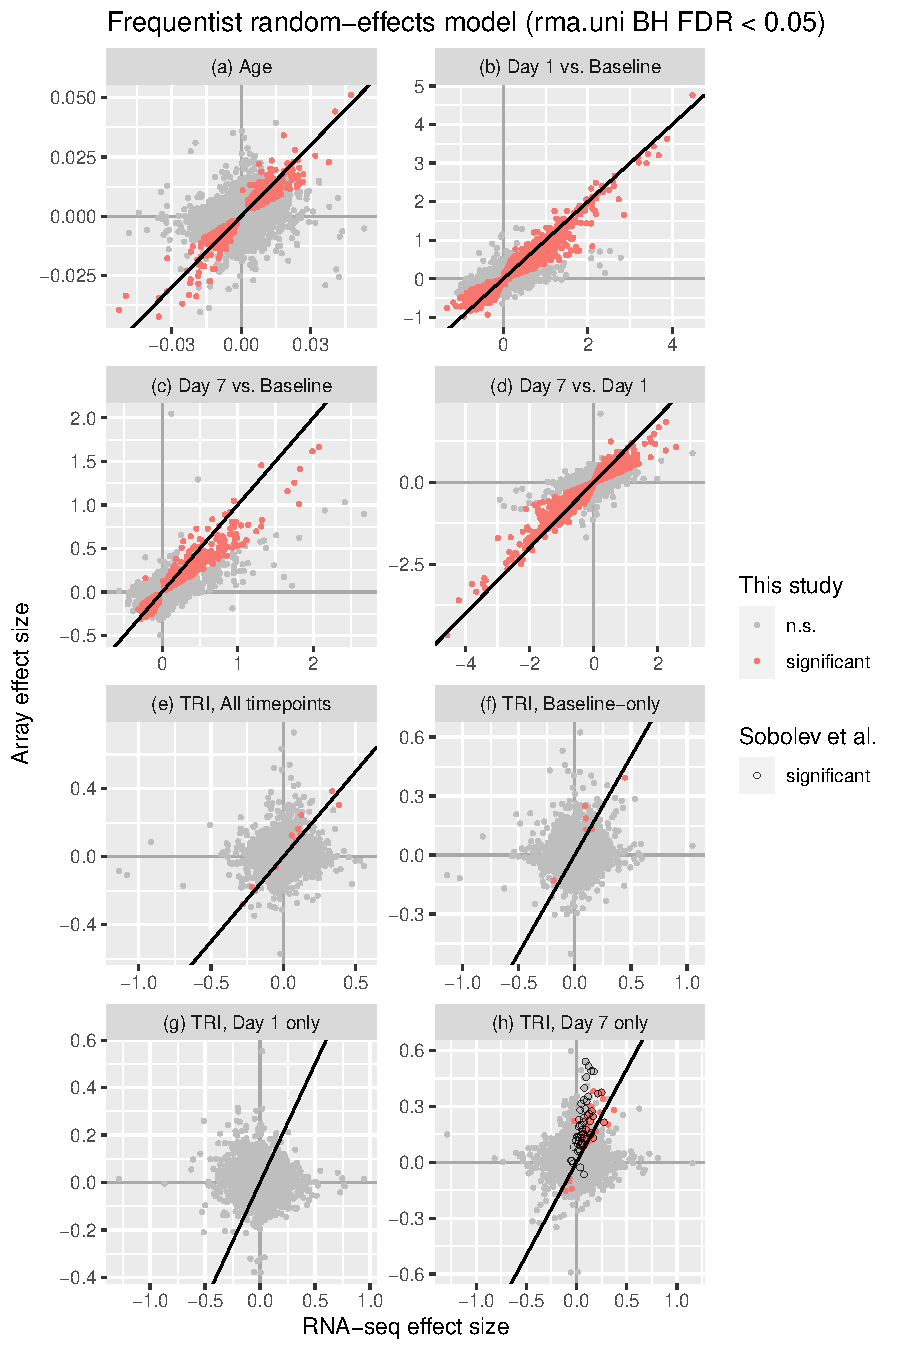
\includegraphics[width=1.0\textwidth,page=1]{mainmatter/figures/chapter_02/plot_dge_eqtl.DGE.effectSizeComparison.pdf}
    \caption{DGE effect sizes estimated in array vs. \gls{RNAseq}. Significance colored by frequentist random effects meta-analysis FDR < 0.05. Genes with day 7 expression associated with responder/non-responder status in \autocite{sobolev2016AdjuvantedInfluenzaH1N1Vaccination} are circled for that contrast.}
    \label{fig:hird_DGE_effectSizeComparisons_rma}
\end{figure}

\begin{figure}
    \includegraphics[width=1.0\textwidth,page=2]{mainmatter/figures/chapter_02/plot_dge_eqtl.DGE.effectSizeComparison.pdf}
    \caption{DGE effect sizes estimated in array vs \gls{RNAseq}. Significance colored by Bayesian random effects meta-analysis lfsr < 0.05. Genes with day 7 expression associated with responder/non-responder status in \autocite{sobolev2016AdjuvantedInfluenzaH1N1Vaccination} are circled for that contrast.}
    \label{fig:hird_DGE_effectSizeComparisons_bayesmeta}
\end{figure}

Significant enrichments were detected at the gene set level; the strongest effects are seen at day 7, where expression of cell cycle, CD4\textsuperscript{+} T cells, and plasma cells are associated with high \gls{TRI}.
At day 0, modules related with inflammatory response in myeloid cells are also associated with high \gls{TRI} (\autoref{fig:hird_tmodDotPlot_TRI}).

\begin{figure}
    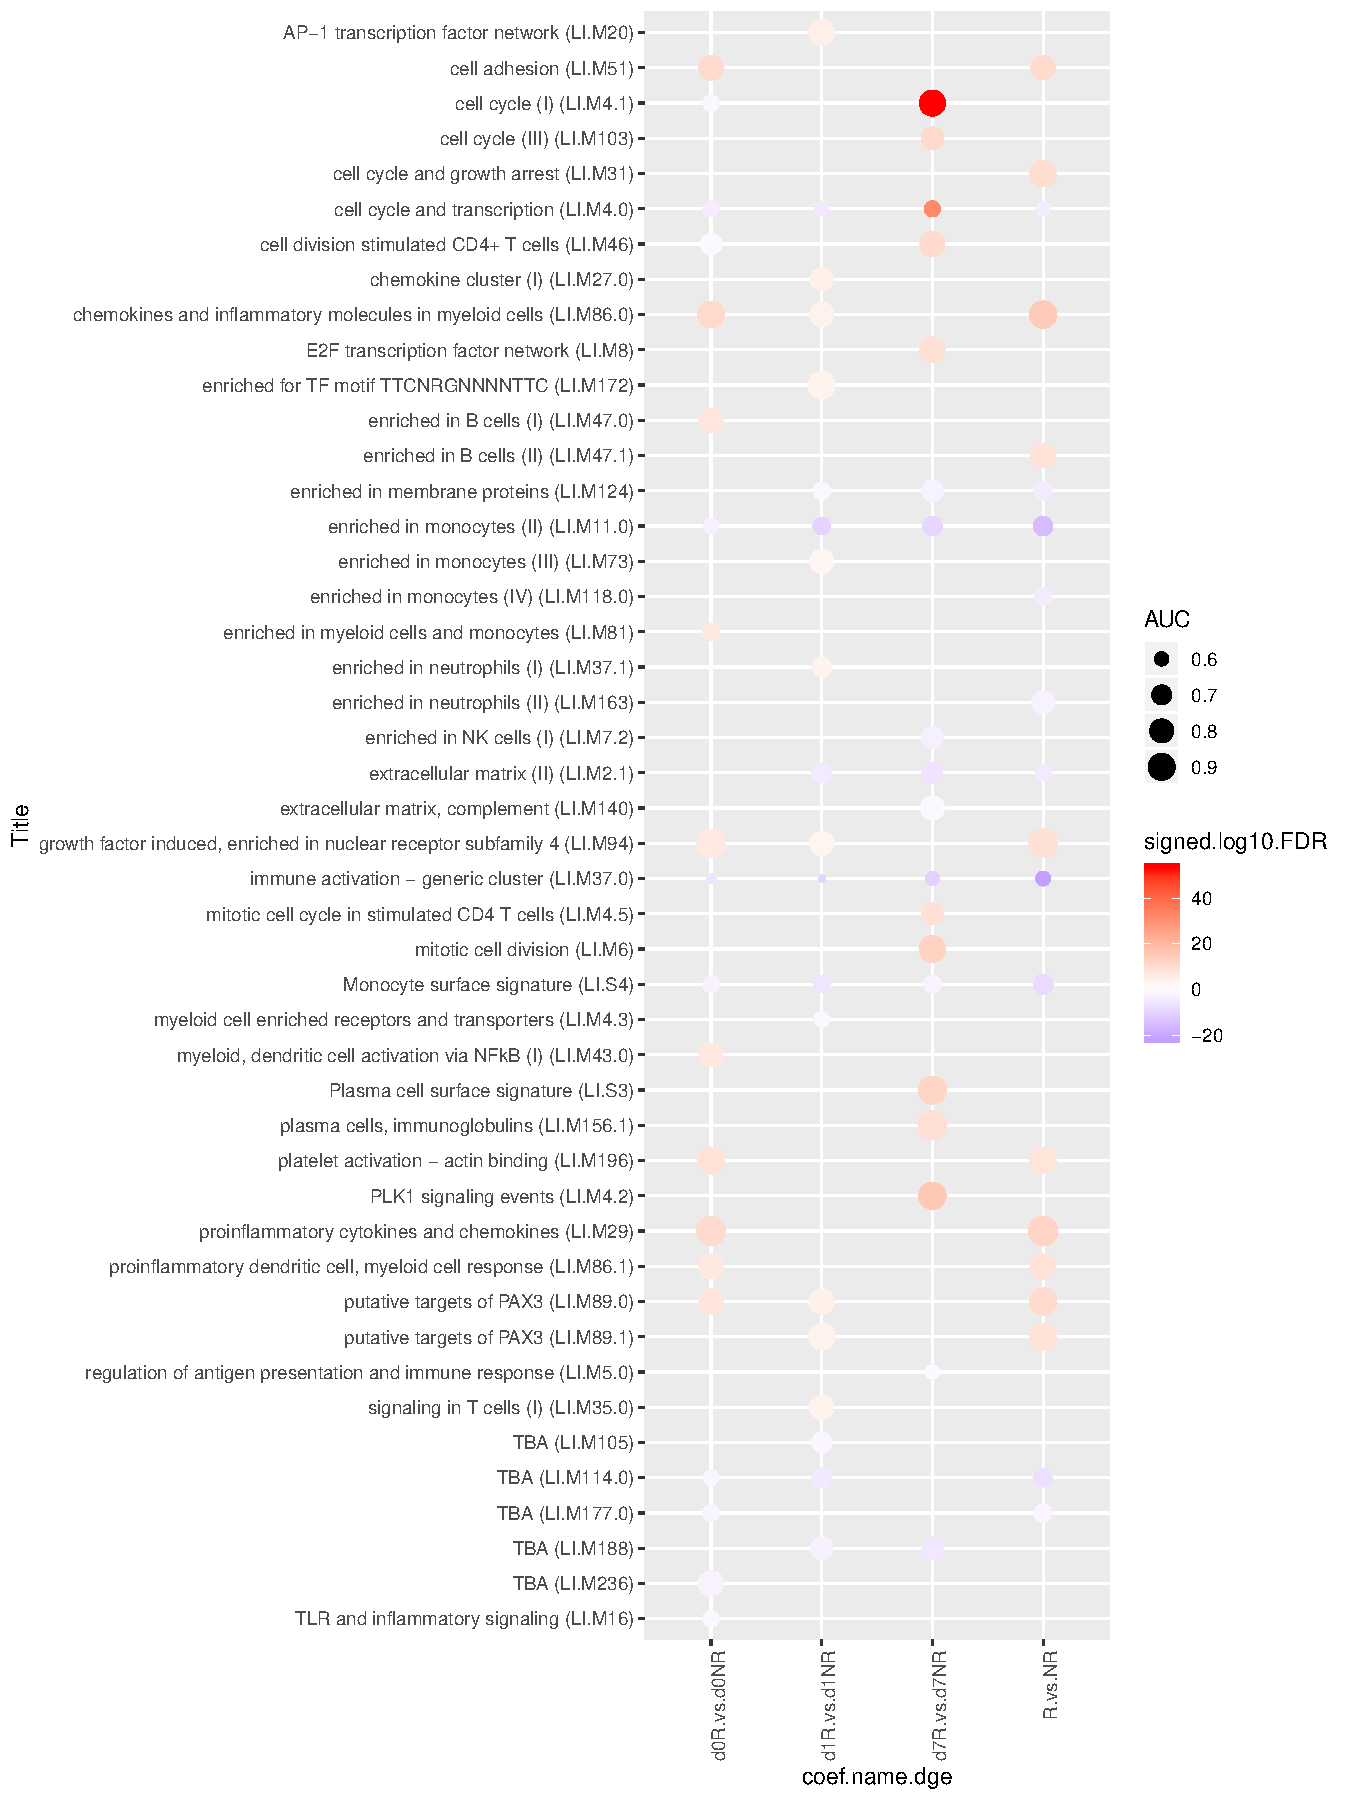
\includegraphics[width=1.0\textwidth]{mainmatter/figures/chapter_02/compare_dge_eqtl.tmodDotPlot.DGE.TRI.pdf}
    \caption{Transcriptomic modules enriched in genes with expression associated with antibody response (\gls{TRI}) at each day. Size of circle indicates effect size. Color of circle indicates significance and direction of effect (red = expression positively correlated with TRI, blue = negative).}
    \label{fig:hird_tmodDotPlot_TRI}
\end{figure}
\todo{figure x labels here should be TRI, not R.vs.NR}

\subsection{Identifying expression signatures for predicting antibody response [probably cut this section and just add to discussion]}

\section{Discussion}

There is extensive transcriptomic response to Pandemrix vaccination in the \gls{HIRD} cohort.
Upregulation of genes and modules related to the interferon signalling pathway, monocytes, inflammatory response, and other aspects of innate immunity were detected at day 1.
This response is transient, with most such genes returning to baseline expression by day 7.
\todo{Not sure if there is a biological interpretion of downreg of T cells and NK cells gene sets at day 1, since it could be due to increase in other cell types in the sample. similar findings in \autocite{nakaya2016SystemsBiologyImmunity} though}
\todo{lit search for downregulation interpretation paper, and downreg T cell paper}
Upregulation of cell cycle/proliferation, activated CD4\textsuperscript{+} T cell, and B (plasma) cell genes and modules were detected at day 7.
This is likely a signature indicating the shift to an adaptive immune response, involving CD4\textsuperscript{+} T cell-supported differention and proliferation of antibody-secreting plasmablasts and plasma cells\autocite{murphy2016JanewayImmunobiology}.
These patterns of expression change between timepoints in the \gls{RNAseq} data are consistent with the patterns in the array data in the original study\autocite{sobolev2016AdjuvantedInfluenzaH1N1Vaccination}, and with expansions of monocyte and plasma cell populations seen in the \gls{FACS} data at days 1 and 7 respectively in the original \gls{HIRD} study\autocite{sobolev2016AdjuvantedInfluenzaH1N1Vaccination}.

In contrast, I was not able to fully replicate the originally reported single gene-level associations between day 7 expression and antibody response in the \gls{RNAseq} data and subsequent and meta-analyses.
In \autocite{sobolev2016AdjuvantedInfluenzaH1N1Vaccination}, 62 genes were reported as differentially expressed between vaccine responders and non-responders.
Although \autocite{sobolev2016AdjuvantedInfluenzaH1N1Vaccination} encodes responder status as a binary phenotype, whereas my analysis uses \gls{TRI}, this is not the primary difference, as 51/62 genes replicated (\gls{FDR} < 0.05) using \gls{TRI} when considering just the array data.
The same analysis using only the \gls{RNAseq} data replicated 0/62 genes.
\todo{might have to rerun everything using the original binary R/NR if this line of reasoning isn't strong enough}
\todo{move numbers to results?}
The majority of the effects for these genes were simply much stronger in the array dataset than in the RNAseq dataset (\autoref{fig:hird_DGE_effectSizeComparisons_rma}).
Given that the range of \gls{TRI} is higher in the array individuals (\autoref{tab:hird_table1}), this does not seem unusual that stronger \gls{TRI}-associated effects are observed there.

58/62 reported hits were measured by both platforms and assessed in the meta-analysis.
Only 15/58 signals replicated using frequentist random-effects meta-analysis to combine per-platform estimates.
I do not consider these hits as robust, as the \gls{REML} estimate of between-platform heterogeneity was zero for 8563/13593 for the day 7 TRI contrast overall, and zero for all 15 of these signals.
None of these signals replicated in the Bayesian random-effects meta-analysis.
The Bayesian meta-analysis is in general more conservative, calling fewer differentially expressed genes compared to the frequentist analysis for all contrasts (\autoref{fig:hird_DGE_effectSizeComparisons_bayesmeta}).
Prior information about $\tau$ is incorporated, discouraging unrealistic estimates of zero heterogeneity.
Given the between-platform heterogeneity coming from both platform-specific technical differences and \gls{TRI} phenotype differences, relative to the modest effect size distributions compared to between-timepoint \gls{DGE} comparisons, the data are not well-positioned to identify significant single-gene associations with antibody response.
%
% Other caveats of the meta analysis
% - The very fact that a meta-analysis is performed adds some bias towards genes with fold changes that can be more consistently measured between platforms; these tend to be genes with higher expression.

% Did we choose the right phenotype?
%
% - the day 63 timepoint is late compared to many other studies
% - Nauta JJ, Beyer WE, Osterhaus AD. On the relationship between mean antibody level, seroprotection and clinical protection from influenza. Biologicals 2009; 37:216-21; PMID:19268607; http://dx. doi.org/10.1016/j.biologicals.2009.02.002 "In clinical studies seroprotection is normally defined as a specific antibody titer or antibody titer increase (seroconversion)."
% - other measures of seroconversion \url{https://www.who.int/biologicals/vaccines/Annex_2_WHO_TRS_963-3.pdf}
% - https://bmcinfectdis.biomedcentral.com/articles/10.1186/s12879-019-4049-5 Seroconversion may not correspond well to protection...

Expression signatures of antibody response were, however, observed at the gene set level, for modules of coexpressed genes that are associated with \gls{TRI} as a whole.
The strongest effects were observed at day 7, where expression of adaptive immune response modules (cell cycle, stimulated CD4\textsuperscript{+} cell, plasma cell modules) were positively associated with \gls{TRI}.
These are the same modules observed to be upregulated at day 7 compared to baseline; it seems that those individuals with the greatest antibody response to vaccination are most able to upregulate these gene sets by day 7 post-vaccination.

Module associations were also observed pre-vaccination (cell adhesion, enriched in B cells, proinflammatory cytokines, platelet activation), suggesting baseline immune state has some influence on long-term antibody response to Pandemrix.
%
% Day 1 TRI ?
% Inflammatory signatures of non-response
% https://www.jacionline.org/article/S0091-6749(17)31766-9/fulltext#sec2.4
% \enquote{The reduced efficacy of vaccination has also been linked to excessive inflammation for influenza,31 yellow fever,32 tuberculosis,33 and hepatitis B34 vaccines.}
%
Over the years, a diverse range of gene sets have been found to be baseline predictors of serological response to influenza vaccination:
    apoptosis\autocite{furman2013ApoptosisOtherImmune}; 
    Fc$\gamma$ receptor-mediated phagocytosis, TREM1 signaling\autocite{tsang2014GlobalAnalysesHuman};
    enriched in B cells, T cell activation\autocite{nakaya2015SystemsAnalysisImmunity};
    B cell receptor signalling, inflammatory response, platelet activation \autocite{hipc-chisignaturesprojectteam2017MulticohortAnalysisReveals}; 
several of which I also observe.
It should be noted that comparisons with these signatures from existing influenza systems vaccinology studies should caveated, as most existing studies are for non-adjuvanted influenza vaccines.
Adjuvanted influenza vaccines are considerably more immunogenic, and post-vaccination expression patterns differ to those of non-adjuvanted vaccines \autocite{sobolev2016AdjuvantedInfluenzaH1N1Vaccination,wilkins2017AS03MF59AdjuvantedInfluenza}.
\todo{could comment on phenotype differences too, i.e. HIRD measure antibodies at d63, much later than is popular in the field: d28 usually}
\todo{should probably emph sobolev didn't find prevacc signatures, and we did. But it's not exactly fair, as sobolev didn't use gene set enrichment as far as i can tell}
Hence, it is particularly important that the robustness of these observed baseline expression signatures be validated in an independent cohort for a comparable AS03-adjuvanted influenza vaccine.

%
% Sobolev:
% Of the volunteers analyzed, essentially all showed expansive changes in peripheral blood gene expression by day 1 (significant changes in ~9,000 gene probes (P < 0.05)) (Supplementary Fig. 2a), highly consistent with other studies that did not use adjuvants8,16,24,25.
% [...]
% In that regard, our study shows that the Pandemrix H1N1 vaccine provokes rapid and expansive, yet transient, activation of myeloid cells and effectors, similarly to changes induced by other vaccines, including flu vaccines lacking adjuvant8,13,15–17. However, our study also reveals a pronounced lymphoid contribution to the early phase of the immune response, most evident in the prominent transient upregulation of IFN-γ, which was not apparent in most other virus vaccine studies.
%
% As noted by \autocite{sobolev2016AdjuvantedInfluenzaH1N1Vaccination}, although the day 1 myeloid response was consistent with studies of non-adjuvanted seasonal influenza vaccines (e.g. \autocite{nakaya2011SystemsBiologyVaccination, bucasas2011EarlyPatternsGene, obermoser2013SystemsScaleInteractive}), the presence of interferon gamma-driven responses was unique to \gls{HIRD}.
% \todo{I think i did not mention specifically type II (IFN-g) in the results section. would need to add HALLMARK set CAMERA results to show this}
%
% Although it is known that AS03 does induce expression changes related to innate immune response at the injection site (\url{https://www.sciencedirect.com/science/article/pii/S0264410X11000399?via%3Dihub#sec0010}), the mechanism of action is unknown (\url{https://www.frontiersin.org/articles/10.3389/fimmu.2017.01760/full}), and there have been relatively few studies of the effect of AS03 or AS03-adjuvanted vaccines on the \gls{PBMC} immune transcriptome aside from the \autocite{sobolev2016AdjuvantedInfluenzaH1N1Vaccination} study itself.
%
% https://www.sciencedirect.com/science/article/pii/S1879625711000769?via%3Dihub#bib0180
% Their mechanism of action remains incompletely understood, however they may amplify immune responses by enhancing antigen presentation and recruiting inflammatory cells to the area of antigen deposition (reviewed in [36]).
%
% https://link.springer.com/article/10.1007/s10875-010-9490-6
% Immune responses to inactivated influenza virus adjuvanted with a different oil-in-water emulsion, MF59, have recently been described [35, 36]. Although a direct comparison between the adjuvants is complicated by the fact that different methodologies may have been used to measure immune responses, our data indicate that AS03A-adjuvanted influenza vaccines induce strong HI responses and CD4 T-cell frequencies relative to those induced with the MF59-adjuvanted product.
%
% AS03-adjuvanted split-virion influenza A/H5N1 vaccine: (\gene{GBP1}, \gene{IRF1}, and \gene{STAT1}) expressions are up in adjuvanted (\url{https://journals.plos.org/plosone/article?id=10.1371/journal.pone.0167488}), three genes that play a role in interferon and antiviral response.
%
% A study of the MF59-adjuvanted \gls{TIV} \autocite{nakaya2016SystemsBiologyImmunity}
%

%
% Sobolev:
% In sum, neither molecular nor cellular data offered any consensus prevaccination predictor of nonresponsiveness akin to those proposed in studies of nonadjuvanted vaccines8,16,17,24,31.
%
% We find some, but...
% - The utility of such signatures is unclear.
% - diagnostics would require prediction
% - and would require protection, not immuno
%
% TODO
\todo{There is also something to be said about 'prediction is not inference'. For use as correlates of protection, as promised by proponents of systems studies, prediction is what is important.}
% - Prediction is not inference tsang2014GlobalAnalysesHuman
%
% For prediction, what rules can be easily implemented in the clinic?
% DAMIP gives rulesets composed of small sets of genes, amenable to rapid qPCR assays.
% We can model HAI and MN in split models. No change scores required.

% Seasonal can prime for H1N1
%
% \2 Efficacy, dosing: \enquote{...a single dose of monovalent 2009 H1N1 vaccine was recommended in adults, but young children were recommended to receive 2 doses (reviewed by [3••]). It is likely that a single dose was sufficient to induce immunity in adults because prior exposure to seasonal H1N1 viruses had immunologically primed the population.}
%
% "Seasonal influenza vaccine provides priming for A/H1N1 immunization." \url{https://www.ncbi.nlm.nih.gov/pubmed/20371459}
%
% Demonstration in a mouse model: \url{https://www.ncbi.nlm.nih.gov/pmc/articles/PMC3024675/}
%
% \2 Inclusion of H1N1 strains into seasonal vaccines
% Sobolev sampled in March 2010 to August 2011
% \2 Later cohorts may have recall response to H1N1 from seasonal vaccination

% - Overall conclusions.
In conclusion, Chapter 2 characterises the expansive changes in \gls{PBMC} gene expression that follow vaccination with Pandemrix.
The dominant trend for all individuals is transient upregulation of the innate immune response at day 1, transitioning into adaptive immunity by day 7.
Baseline-adjusted antibody response is correlated with expression of gene sets, particularly adaptive immunity modules at day 7, but also for some modules pre-vaccination.
Unfortunately, between-platform variation in expression impedes identification of specific genes that contribute.
The fundamental question of why gene expression and antibody responses vary between \gls{HIRD} individuals remains.
Chapter 3 will examine one hypothesis: the impact of common human genetic variation on Pandemrix expression response.
\todo{found signatures, but so what? Feels like chapter lacks a punchline?}

\todo{why blood? ready easy supply of immune cells}


% HIRD reQTLs
%
% Chapter 3
%
% Response eQTL-style HIRD paper

\chapter{Genetic architecture of transciptomic response to Pandemrix vaccine}
\label{ch:hird_reQTL}

\textit{
    The work presented in this chapter is a collaboration between 
    the Wellcome Sanger Institute,
    King's College London, 
    the Francis Crick Institute,
    and the Biomedical Research Centre at Guy's and St Thomas' Hospital and King's College London.
    I would like to reiterate my thanks to the people and organisations mentioned at the beginning of \cref{ch:hird_DGE}.
}

\section{Introduction}

\subsection{Host genetic factors affecting influenza vaccine response}
\label{subsec:hird_reQTL_intro_geneticFactorsFluVaccine}

Many human traits are heritable and complex---response to vaccination is no exception.
Twin studies have demonstrated approximately \SIrange{30}{90}{\percent} heritability of antibody responses to many vaccines, including smallpox, hepatitis A and B, anthrax, pneumococcal, \textit{Haemophilus influenzae} type b (Hib), diphtheria-tetanus-pertussis (DTP), Bacillus Calmette--Guérin (BCG) \autocite{mooney2013SystemsImmunogeneticsVaccines,oconnor2013CharacterizingVaccineResponses,newport2015GeneticRegulationInfant,brodin2015VariationHumanImmune}.
Candidate gene studies and \glspl{GWAS} have identified multiple genetic associations with antibody response \autocite{mooney2013SystemsImmunogeneticsVaccines,oconnor2013CharacterizingVaccineResponses,mentzer2015SearchingHumanGenetic,linnik2016ImpactHostGenetic}, 
including replicated associations 
for hepatitis B vaccine in a haplotype block in the \gls{HLA} region encompassing \gene{HLA-DR} and \gene{BTNL2},
and for measles vaccine in an intron of a receptor known to interact with measles virus, \gene{CD46}.

In contrast, \textcite{brodin2015VariationHumanImmune} found anti-\gls{HA} antibody responses to seasonal influenza vaccine in 105 adult twin pairs (median age, \SI{44}{\year}) had no detectable heritabilty,
alongside a general decrease in heritability of most immune parameters with age.
They posited 
that the genetic contribution to response was overshadowed by environmental factors such as previous influenza vaccination or infection in adults, 
whereas the estimated heritability of the aforementioned vaccines was substantial
because they are vaccines against non-circulating pathogens, 
or are childhood vaccines for which heritability was assessed in young children with shorter immune history.

Nevertheless, a small number of candidate gene studies have identified genetic variants associated with antibody response to influenza vaccines \autocite{linnik2016ImpactHostGenetic}.
\textcite{gelder2002AssociationsHumanLeukocyte} ($n=73$) identified associations between \gls{HLA} alleles in \gene{HLA-DRB1} and \gene{HLA-DQB1} with \gls{HAI} seroconversion after \gls{TIV};
\textcite{moss2013CorrelationHumanLeukocyte} ($n=185$) also found associations between \gls{HLA} class II alleles (HLA-DRB1*04:01 and HLA-DPB1*04:01) and \gls{HAI} seroconversion after seasonal influenza vaccination.
\textcite{poland2008ImmunogeneticsSeasonalInfluenza} ($n=184$) tested HLA alleles, and \glspl{SNP} in coding and regulatory regions of cytokine or cytokine receptor genes, for association with post-\gls{TIV} \gls{HAI} titres specific to H1 and H3 subtypes (two of the components in the trivalent vaccine).
They reported nominally significant associations for two \gene{HLA-A} alleles with H1-specific titres,
six \glspl{SNP} associations with H1-specific titres
and ten \glspl{SNP} associations with H3-specific titres.
\textcite{egli2014IL28BKeyRegulator} ($n=196$) identified a \gls{SNP} upstream of \gene{IFNL3} (rs8099917) to be associated with seroconversion post-\gls{TIV},
and also found the \gls{SNP} to be an \gls{eQTL} for \gene{IFNL3} expression in H1N1-stimulated \glspl{PBMC} in a second cohort ($n=49$).
Lastly, \textcite{avnir2016IGHV169PolymorphismModulates} focused on a coding variant (rs55891010) in the part of \gene{IGHV1-69} that encodes the \gls{CDR} of broadly neutralising antibodies that bind influenza \gls{HA}.
One month after H5N1 avian influenza vaccination ($n=85$), associations were detected with usage of \gene{IGHV1-69} in the antibody repertoire,
and serum antibody binding efficiency to H5N1 \gls{HA}.
The associations listed above have all been found in small cohorts and have not been validated by subsequent studies,
so it remains unknown whether robust genetic associations with antibody response to influenza vaccines exist.

% NOTE: never mind the cellular response
%
% Genetics affects cellular response to other vaccines.
% DOI: 10.1128/CMR.00084-18
% Different ethnic groups living in the same location have varied responses to vaccination (64, 89, 161–166) and decline of antibodies (89), indicating a genetic influence on vaccine responses. Studies of twins estimate the degree of heritability to be 36 to 90% for humoral responses (167–173) and 39 to 90% for cellular responses, depending on the specific vaccine (167, 169) (Table 3).

% Adverse events genetics
% Also, genetics of phenotypes such as adverse events have been studied e.g. \url{https://pubmed.ncbi.nlm.nih.gov/25344690/}, ollila2017GeneticsVaccinationrelatedNarcolepsy

\subsection{\Glsfmtfullpl{reQTL} following influenza vaccination}

Host genetic variation could play a causal role in influenza vaccine response by altering the expression of genes as \glspl{eQTL}.
As mentioned in \cref{subsec:intro_contextDependenteQTL} and \cref{subsec:intro_reQTL}, the effect sizes of \glspl{eQTL} can be highly context-dependent,
and many \glspl{eQTL} in the immune system are \glspl{reQTL} only detectable after stimulation, not at baseline.
% \gls{eQTL} can have condition-specificity: an interaction between their effect on expression and different environmental contexts such as tissue or cell type\autocite{albert2015RoleRegulatoryVariation,vandiedonck2017GeneticAssociationMolecular}.
% The mechanisms by which \glspl{eQTL} interact with environment are of great interest;
% for example, cell type-specificity can inform us about how expression is regulated in a cell type-specific manner\autocite{kim-hellmuth2020CellTypeSpecific}.
% In a vaccination context, an important subset of context-dependent
% environment-interacting eQTLs are \glspl{reQTL}, defined as an eQTL whose effect interacts with external stimulation or perturbation.
% As the pre- and post-stimulation environments are separated in time, a possible mechanism that leads to the observation of reQTL is a genotype-dependent change in gene expression between timepoints,
% which may underlie genotype-dependent differences in antibody phenotypes.
\Glspl{reQTL} can be mapped considering a vaccination as an \textit{in vivo} immune stimulation.
This usually involves measuring the transcriptome of immune cells before and after vaccination in genotyped individuals,
then testing for genotype-dependent changes in expression.
As expression is a key molecular intermediate between genotype and phenotype,
a genotype-dependent change in expression after vaccination may be a mechanism mediating genotype-dependent vaccine antibody responses.

As reviewed in \cref{subsec:intro_reQTL},
few \textit{in vivo} \gls{reQTL} studies have been conducted,
and even fewer studies have been conducted where the \textit{in vivo} stimulation is vaccination,
despite the potential for learning about genetic regulation of vaccine-induced expression responses.
To my knowledge, there is only one such study: by \textcite{franco2013IntegrativeGenomicAnalysis} on response to seasonal inactivated \gls{TIV}.
\textcite{franco2013IntegrativeGenomicAnalysis} enrolled healthy Europeans adults into discovery ($n=119$ males) and validation ($n=128$ females) cohorts in two consecutive influenza seasons\footnote{Sex-dependence of effects was not addressed.}.
In each cohort, peripheral blood gene expression was measured by expression array on day 0 (baseline); and on days 1, 3, and 14 post-vaccination.
Serum \gls{HAI} and \gls{MN} titres were measured at days 0, 14, and 28 against each of the three vaccine components.
The \gls{TRI} \autocite{bucasas2011EarlyPatternsGene} was computed from these titres as a single measure of antibody response adjusted for baseline titres.
Genotyping was done by genotyping array.

\textit{Cis}-\gls{eQTL} were mapped using a linear mixed model jointly over all four days,
with day, genotype, day-genotype interaction, and a random intercept for individual as predictors; and gene expression the response variable.
This resulted in 467 (non-independent) \gls{eQTL} for 78 genes replicated in both cohorts,
with a significant day effect (indicating the gene was differentially expressed post-vaccination)
and a significant genotype effect (indicating the \gls{eQTL} effect).
To call \glspl{reQTL}, \glspl{eQTL} were also mapped separately for each day with a linear model including only genotype as a predictor,
from which the model $R^2$ was computed as a rough measure of the variance in expression explained by the \gls{eQTL} at each day.
\textcite{franco2013IntegrativeGenomicAnalysis} then computed delta-$R^2$: the maximum absolute deviation of the three post-vaccination $R^2$s from the day 0 $R^2$.
Out of the \glspl{eQTL} that replicated in both cohorts, 
146 \glspl{eQTL} for 34 genes ranked above the 99th percentile of the delta-$R^2$ distribution were defined as \glspl{reQTL}.
The union of the 78 and 34 genes from the above analyses (98 genes with \gls{DGE} and an \gls{eQTL}; or a \gls{reQTL}) was enriched for pathways and gene sets related to  
antigen processing and presentation, CD8\textsuperscript{+} T cell-mediated apoptosis, \gls{DC} maturation and function, and membrane trafficking.

Lastly, integrating antibody titre data,
they filtered down to 20 genes with expression correlated to \gls{TRI} at any day, 
with an \gls{eQTL}, 
and with either post-vaccination differential expression \emph{or} a \gls{reQTL} effect.
% Their written conclusion was that: \enquote{these [20] loci have the strongest evidence of genetic variation influencing the immune response to the vaccine}, but due to the final \enquote{or} in their filtering criteria...
% TAP2, SNX29, FGD2, NAPSA, NAPSB, GM2A, C1orf85, JUP, FBLN5, CHST13, DIP2A, PAM, D4S234E, C3AR1, HERC2, LST1, LRRC37A4, OAS1, RPL14, and DYNLT1.
Seven genes out of these 20 were involved in antigen transport, processing, or presentation in \glspl{APC}:
\gene{NAPSA}, \gene{C1orf85}, \gene{GM2A}, \gene{SNX29}, \gene{FGD2}, \gene{TAP2}, and \gene{DYNLT1}.

Critically, \textcite{franco2013IntegrativeGenomicAnalysis} recognised that just assessing overlap of multiple filtering criteria does not allow them to infer the direction of causal relationships between genetic variation, expression and \gls{TRI}.
They attempted a model comparison with the CIT \autocite{millstein2009DisentanglingMolecularRelationships} to resolve the directionality of association between expression and \gls{TRI}, 
finding suggestive evidence of causal effect on \gls{TRI} mediated by expression at several \gls{eQTL}.
Unfortunately, they also evaluated that the power of the CIT was only \textapprox{\SI{60}{\percent}} at their total sample size of $n=247$.
Nevertheless, the study is proof of concept that integration of genotype, expression and antibody response data in an \textit{in vivo} \gls{reQTL} framework can be of suggestive genes under genetic regulation likely to be involved in vaccine response.

\subsection{Chapter summary}

The \gls{HIRD} cohort represents a unique opportunity for detecting genetic contributions to influenza vaccine response.
Similar to \textcite{franco2013IntegrativeGenomicAnalysis},
expression, antibody response, and genotypes are all available for the same individuals.
As Pandemrix is against a pandemic strain that had not been in seasonal circulation for decades at the time of cohort recruitment, 
responses will be less driven by individual immune history,
so power to detect genetic associations is expected to be greater.
% The cohort is too small for GWAS, so here expression.
% The only genetic factor measured was HLA haplotype, which did not associate with any other parameters measured.
In \cref{ch:hird_DGE}, I characterised differential gene expression induced by Pandemrix, as well as expression associations with antibody titres.
% For seasonal influenza vaccines, the contribution is small: antibody responses in adults are largely driven by non-genetic influences such as previous influenza vaccination or infection\autocite{brodin2015VariationHumanImmune}.
% As the Pandemrix vaccine is against a pandemic strain that was not in seasonal circulation at the time the \gls{HIRD} cohort was recruited (2010-11),
% with individuals mounting an expression response that was not recall-dominated \autocite{sobolev2016AdjuvantedInfluenzaH1N1Vaccination},
% the relative contribution of genetic factors to Pandemrix response may be greater.
In this chapter---given that \gls{HIRD} is too small for a direct \gls{GWAS} of antibody response---I focus on the genetic contribution to expression response.
I apply the \textit{in vivo} \gls{reQTL} framework, 
aiming to characterise the association of common genetic variants with expression across multiple timepoints,
and pinpoint genes important to Pandemrix response.
% I map cis-\gls{eQTL} within each timepoint, accounting for ancestry, cell type composition, and unmeasured covariates, then call shared and \gls{reQTL} effects across timepoints from a joint model.
% Many of the strongest reQTL effects involve opposite signed effects on expression for the same variant at different timepoints.
% I detect a strong day 1 specific reQTL effect at \gene{ADCY3}.
% Through modelling interaction of reQTL with cell type abundance estimates and statistical colocalisation with cell type-specific QTL datasets,
% the reQTL signal was determined to be a monocyte-specific effect likely driven by increase monocyte abundance at day 1.

\section{Methods}
\label{sec:hird_reQTL_methods}

\subsection{Overall strategy for \glsfmtshortpl{reQTL} mapping}
\label{subsec:hird_reQTL_overall_strategy}

A plethora of approaches to mapping \glspl{eQTL} with linear models exist; each with its own advantages, disadvantages, and assumptions.
When the task is also to define \gls{reQTL} between multiple conditions, the diversity of possible approaches multiplies further.
Here I will discuss aspects of the data and available methodologies that led to the final modelling strategy in this study.

\subsubsection{Adjusting for population structure using \glsfmtlongpl{LMM}}

Population structure occurs when the samples in a study are not independent, but structured due to genetic relatedness.
Genetic association studies assume that the individuals in a sample are unrelated (or at least sufficiently distantly related) \autocite{astle2009PopulationStructureCryptic,sillanpaa2011OverviewTechniquesAccount,sul2018PopulationStructureGenetic}.
Relatedness, and thus population structure, occurs at different scales.
Population stratification refers to systematic differences in allele frequencies and genetic background between human populations due to demographic history.
This represents large-scale structure where individuals are related due to shared ancestry \autocite{price2010NewApproachesPopulation,sillanpaa2011OverviewTechniquesAccount}.
At a smaller scale, sample individuals can be related due to being in the same family.
The presence of more relatedness in a sample than is assumed is the problem of cryptic relatedness \autocite{astle2009PopulationStructureCryptic,sillanpaa2011OverviewTechniquesAccount,sul2018PopulationStructureGenetic};
this can be at any scale, but more often the term refers to recent relatedness.
% NOTE: fine scale population structure
% If one assumes humans across the globe are a single randomly mating population, it would result in only a 5–15% average error when predicting the proportion of observed heterozygotes at a locus. This closeness to an idealized randomly mating population is one vestige of how little evolutionary time has passed since the common origin of all humans in Africa. The departure from random mating predictions due to population differentiation has a classic quantitative measure, called FST, which appropriately takes on values of 5–15% in global samples of human populations [1, 2, 3••]. If one zooms in within continental regions of the globe, FST tends to be even lower, regularly taking values below 1%, a threshold which we use here informally to define ‘fine-scale structure’.

In the context of \gls{eQTL} mapping (and genetic association studies in general), 
where the aim is to assess the effect of a single genetic variant on expression, 
there is potential for confounding.
The issue (also reviewed elsewhere \autocite{sul2018PopulationStructureGenetic,golan2018MixedModelsCaseControl}) is that we fit a marginal model to estimate the effect of a single variant $x_k$ on the phenotype $y$:
\begin{equation}
    y = \mu + \beta_k x_k + \epsilon
    \label{eq:hird_reQTL_gwas_model_marginal}
\end{equation}
where $\mu$ is the intercept,
and $\epsilon \sim N(0, \sigma_e^2 I)$ is the error term that represents environmental and stochastic sources of variation,
The variance-covariance matrix for error term is a scalar matrix, 
encoding the classic regression assumptions of homoscedasticity and uncorrelated errors.
A more appropriate data generating model is:
\begin{equation}
    y = \mu + \beta_k x_k + G + \epsilon
    \label{eq:hird_reQTL_gwas_model_full}
\end{equation}
where $G = \sum_{i \neq k}{\beta_i x_i}$ represents the effect of the genetic background at all other variants.
As many variants can be expected to affect a complex polygenic trait, $G$ has some causal effect on $y$.
Population structure means there can be a shared cause of $G$ and $x_k$ such as ancestry.
This opens a backdoor path $x_k \leftarrow \text{ancestry} \rightarrow G \rightarrow y$,
confounding the relationship between $x_k$ and $y$.
In \cref{eq:hird_reQTL_gwas_model_marginal},
% the error term will actually represent $G + \epsilon$.
% the error term and $x_k$ become correlated (endogeneity),
when one estimates the coefficients,
the effects of the omitted variable $G$ will be attributed to $x_k$,
resulting in spurious associations and genomic inflation of test statistics \autocite{price2010NewApproachesPopulation}.
Here, $G$ represents exactly the confounding due to genetic background,
but there are other possible confounders,
such as shared environmental factors that differ systematically between populations \autocite{vilhjalmsson2013NatureConfoundingGenomewide}.
A popular approach to avoid confounding is to include genotype \glspl{PC} as fixed effects in the regression \autocite{price2006PrincipalComponentsAnalysis,eu-ahsunthornwattana2014ComparisonMethodsAccount},
thus blocking the backdoor path from $x_k$ to $y$.
Genotype \glspl{PC} represent population stratification effects like ancestry, 
but also act a proxy to block confounding by genetic background and environmental effects \autocite{vilhjalmsson2013NatureConfoundingGenomewide}.

Unfortunately, genotype \glspl{PC} alone cannot account for smaller-scale population structure \autocite{price2010NewApproachesPopulation}.
An approach that can explicitly model such population structure is the \gls{LMM} \autocite{price2010NewApproachesPopulation,eu-ahsunthornwattana2014ComparisonMethodsAccount,golan2018MixedModelsCaseControl},
which expresses the idea that more genetically correlated individuals are expected to be more phenotypically correlated \autocite{vilhjalmsson2013NatureConfoundingGenomewide}.
A typical model form is:
\begin{equation}
    y = \mu + \beta_k x_k + u + \epsilon
    \label{eq:hird_reQTL_gwas_model_lmm}
\end{equation}
where random effect $u \sim N(0, \sigma_g^2 K)$
has a variance-covariance matrix proportional to the genetic correlation between individuals, the kinship matrix $K$.
% Since the SNPs are correlated, due to the major genome-wide diffrences in allele frequencies between the populations, this results in a correlation between the tested SNP and the noise term.
This improves on \cref{eq:hird_reQTL_gwas_model_full} by recognising that the variants in $G$ are correlated.
$\sigma_g^2$ is often called the variance component; the larger it is, the more phenotypic variance is explained by genetic background \autocite{golan2018MixedModelsCaseControl}.
Although \glspl{LMM} were originally developed in the context of animal breeding, where $K$ is computed from a known pedigree,
it can also be estimated from genome-wide \gls{SNP} data \autocite{eu-ahsunthornwattana2014ComparisonMethodsAccount,sul2018PopulationStructureGenetic}.
Unlike pedigree‐based kinships that range from 0 (unrelated) to 1 (self or identical twin),
\gls{SNP}-based relatedness values represent average correlations of alleles between individuals \autocite{speed2017ReevaluationSNPHeritability},
hence may be negative or greater than 1 \autocite{wang2014MarkerbasedEstimatesRelatedness}
This does not affect their usage in \glspl{LMM}.
%
% Also see: 
%
% 2018-11-26 notes in log
%
% https://twitter.com/A_A_Zaidi/status/1285578961356034049
% When structure has a recent origin, PCA or LMMs won't fully correct for stratification if the GRM is derived from common variants as they are older and not very informative about recent demographic history.
%
% We demonstrate that widely used approaches to adjust for population structure, including principal components analysis and mixed modelling with a random effect for a genetic relationship matrix, cannot fully account for the fine-scale geographical confounding in the UK Biobank.
% fine scale: https://academic.oup.com/hmg/article-abstract/doi/10.1093/hmg/ddaa157/5874041

In \gls{HIRD},
the genotype data were already filtered such that no pair of individuals are first-degree relatives or closer (\cref{subsec:hird_dge_genotype_preproc}),
but cryptic relatedness might remain.
The multi-ethnicity of the cohort means there is large-scale population structure from ancestry (\cref{fig:hird_genotype_pca_withHapmap}).
Genotype \glspl{PC} were computed to represent axes of variation due to ancestry.
These were included as covariates in \gls{DGE} analyses in \cref{ch:hird_DGE} to improve efficiency by explaining some variation in expression.
For \gls{eQTL} mapping in this chapter, I use both a random effect in an \gls{LMM} and \gls{PC} fixed effects to correct for population structure.
This may not be strictly necessary if the random effect can correct for large-scale structure, 
but does not seem to impact power or type I error rate \autocite{widmer2015FurtherImprovementsLinear},
and may have some benefits at \glspl{SNP} with very different allele distributions between populations (unusually differentiated) \autocite{price2010NewApproachesPopulation}.

% For list of various methods considered, also see 2018-03-05, 2018-07-25, 2018-07-27 etc. in log
The performance of various software implementations 
for kinship estimation from genome-wide \gls{SNP} data and \glspl{LMM} are highly comparable; 
the specific choice of implementation can usually be made on the basis of computational efficiency \autocite{eu-ahsunthornwattana2014ComparisonMethodsAccount}.
In this chapter, I use
\glspl{LMM} implemented in \software{LIMIX} \autocite{lippert2014LIMIXGeneticAnalysis}
with kinship matrices estimated by \software{LDAK} \autocite{speed2012ImprovedHeritabilityEstimation}.

\subsubsection{Multi-condition models}

Since the aim of this chapter is to identify genetic variation that affects expression response to vaccination, it may seem most direct to model the change in each individual's expression after vaccination as the response variable.
This approach has been applied for identification of condition-specific \gls{eQTL}, typically with the response taking units of log fold change between conditions (e.g. \autocite{maranville2011InteractionsGlucocorticoidTreatment,ackermann2013ImpactNaturalGenetic,shpak2014EQTLAnalysisHuman}).
Although potentially powerful if \gls{eQTL} effects are small and opposite between conditions\autocite{ackermann2013ImpactNaturalGenetic}, 
% TODO: although ackermann2013ImpactNaturalGenetic distinguishes dynamic, there is no structural diff between using the
% fold change vs interaction vs stratified, for example, suppose different individuals pre and post, it's really a matter of assumptions and efficiency.
it is analogous to the \enquote{change score} approach, which can suffer from regression to the mean, and increased uncertainty from the variance sum law if effects between conditions have positive covariance\autocite{allison1990ChangeScoresDependent,clifton2019CorrelationBaselineScore}.
% NOTE:
% https://journals.sagepub.com/doi/full/10.1177/1054773816666280
% Threats to Its Internal Validity and External Validity of One-Group Pretest–Posttest Design include regression to the mean.
%
% Step 1: why not intra-individual change score, why not ANCOVA, why strat and diff?
% half a century of debate
% https://digscholarship.unco.edu/cgi/viewcontent.cgi?article=1239&context=dissertations
% https://ruor.uottawa.ca/bitstream/10393/35843/3/Lemay_Julien_2017_Thesis.pdf

% TODO:
% in observational: https://www.tandfonline.com/doi/abs/10.1080/00273171.2013.831743?scroll=top&needAccess=true&journalCode=hmbr20
% in RCT: senn says equiv: https://www.google.com/url?sa=t&rct=j&q=&esrc=s&source=web&cd=&ved=2ahUKEwie_PK6vsvsAhXXRRUIHdUfD_wQFjAAegQIAxAC&url=http%3A%2F%2Fimaging.mrc-cbu.cam.ac.uk%2Fstatswiki%2FFAQ%2Frt1d%3Faction%3DAttachFile%26do%3Dget%26target%3Dsenn.ppt&usg=AOvVaw0Rp28syfyesdecEiQZw9x_
% pearl says: ?
% senn in observational: ?? https://onlinelibrary.wiley.com/doi/abs/10.1002/sim.2682
%
% \todo{upend change score bit, here expression is a y variable. compare all the options as glms etc.}
% TODO: Write both as special cases of glm, and highlight their different assumptions
% TODO: mention: in ch2, used residualised change score, here, different
% Our data structure is
% Over all approach is stratified
%
% 2 schools of thought. 50 years of debate
% Change score assigns special status, assumes a specific correlation
% ...
%
% Besides not even estimatejng the same effect
%
% Many other models reduce to change score
%
% Mixed is flexible, but overall aim aligns with change score
%
% Simplest application of developed eqtl methods

% joint method over interaction
%     large numbers of conditions, not practical to use interactions

% pros for split
%     limix not ok with repeated samples in kinship matrix
%     peer not directly applicable
    
% change score should ask average of individual diffs
% strat and interaction should ask diff in averages
% interaction is further borrowing info
%
% NOTE: see
% Senn: Statistical Issues in Drug Development
% 7.2.4 Is clinical relevance a relevant consideration when choosing whether to use change scores or raw outcomes as the efficacy measure?

% TODO:  
 % It is imperative to adjust for the baseline value anyway, using regression modeling (for reasons of bias reduction in observational studies and for maximizing power and precision in randomized trials).
 % Using each patient as her own control through calculation of a change score is worse than using no control if the baseline is noisy. If the correlation between baseline and follow-up measurement is less than 0.5, subtracting the baseline is worse than just analyzing the follow-up measurement.
 % http://biostat.mc.vanderbilt.edu/wiki/Main/MeasureChange

Instead, I map \glspl{eQTL} within each of three timepoint conditions (day 0 pre-vaccination, day 1, and day 7), and find \glspl{reQTL} by looking for \glspl{eQTL} that have different effects between conditions.
% TODO: would use ANCOVA here i.e. equiv to continuous covar in regression
% TODO it is not the case people act as their own controls, you can't observe the counterfactual outside of n of 1 trials
% more like soaking up some of the variation as within individual random effect, allowing more precise
% also see: https://blog.statsols.com/making-it-personal-n-of-1-trials-allowing-for-individuality-but-not-overdoing-it
% \todo{Can this really demonstrate genotype-dependent change in gene expression between timepoints? i.e. need understand how the change score/ANCOVA approaches differ from repeated measures ANOVA differ from the interaction/stratified approach I take?}
Unlike a test for difference implemented using a genotype-condition interaction term in a joint regression model, homoscedasticity of errors is not assumed for all conditions\autocite{clogg1995StatisticalMethodsComparing}
% See PMC4425538 : The method we have used did not account for heteroscedasticity while estimating the standard errors of the interaction term, which may lead to inflated statistics.
% TODO: equivalence is not straightforward, since of joint mashr downstream

% real killer is missing data for manova/ancova
% TODO: also MANOVA
% Instead of just accommodating unequal variances and covariance within a subject, the mixed models approach directly models the covariance structure of the multiple dependent variables.
% https://blogs.sas.com/content/sastraining/2011/02/02/the-punchline-manova-or-a-mixed-model/
% https://stats.stackexchange.com/questions/13197/differences-between-manova-and-repeated-measures-anova
% avoids sphericity http://www.discoveringstatistics.com/docs/sphericity.pdf
%
% But, we are interested in interaction, and this is not directly answered by manova (i.e. multivariate mode in limix)

% Independence: errors assoc with one observation are not correlated with erros of any other
% Homoscedasticity: Var y does not depend on x

% Step 2: why stratification/subgroup not interaction
% TODO interaction is more efficient under certain assumptions
%     https://stats.stackexchange.com/questions/332963/why-may-results-from-model-with-interaction-term-and-stratified-model-be-differe
% These models will consistently estimate the same thing only when the mean model is true.
% possible here since time is not treated as continuous
% https://stats.stackexchange.com/questions/93540/testing-equality-of-coefficients-from-two-different-regressions
    % I found the key difference is whether the assumption that the error variance is the same or not.
% https://stats.stackexchange.com/questions/55501/test-a-significant-difference-between-two-slope-values
    % The classic (and more statistically powerful) way of testing this is to combine both datasets into a single regression model and then include the area as an interaction term. See, for example, here:
    % http://www.theanalysisfactor.com/compare-regression-coefficients/
    % This is "more ... powerful" only if more restrictive assumptions apply. In particular, it assumes homoscedasticity of error variances. Often one would not want to assume that (without additional justification) and therefore would use something like the Welch or Satterthwaite t-test. – whuber♦ Mar 30 '16 at 21:46
%
% https://stats.stackexchange.com/questions/33692/joint-model-with-interaction-terms-vs-separate-regressions-for-a-group-comparis
%     The first model will fully interact gender with all other covariates in the model. Essentially, the effect of each covariate (b2, b3... bn). In the second model, the effect of gender is only interacted with your IV. So, assuming you have more covariates than just the IV and gender, this may drive somewhat different results.
% i.e. there are interactions between time and ALL VARIABLES
%
% whereas interaction model pools estimates (borrows info)
%
% cons:
% interaction gives direct p nominal value, we have to estimate
% but how to control for multiplicity?
%
% Statistical Approaches for Estimating Sex-Specific Effects in Endocrine Disruptors Research
% https://ehp.niehs.nih.gov/doi/10.1289/EHP334 < TODO
%
% also see homo: https://cris.maastrichtuniversity.nl/ws/files/11868404/799719.pdf
% TODO:
% really, pro is Simplicity
% Can do interactions
% Can do coloc
% Can use peer
% interaction with time fixed fx vs stratified
% \todo{interactions, apart from scalability genome wide, and additional complexity when also adding cell type and platform interactions, and assumption of homoscedascity between all groups}
% vs pooling power
%
% note intent to use joint modelling later, so as to not lose info and fall into jelly bean problem https://www.ahajournals.org/doi/10.1161/CIRCULATIONAHA.108.836601

% TODO: honestly given i used change score in ch2, the biggest motivator is probably practicality e.g. ability to use PEER

%
% DEPRECATED:
% How to meta-analyse? We are restricted to non-full Bayesian methods.
%
% See last paragraph of discussion in
% Kontopantelis, E., Springate, D. A., & Reeves, D. (2013). A Re-Analysis of the Cochrane Library Data: The Dangers of Unobserved Heterogeneity in Meta-Analyses. PLoS ONE, 8(7), e69930. https://doi.org/10.1371/journal.pone.0069930
% For small k, Sidik MVa or Ruhkin RBp recommended.
%
% metafor manual
% If, instead of the crude estimate, one wants to use a better apriori estimate, one can do so by passing this value via control=list(tau2.init=value)
% Sidik-Jonkman estimator, also called the ‘model error variance estimator’, is implemented in metafor (SJ method).
% Starts with an init estiamte of ri=sigma2i/tau2i i.e. ratio of study-specific and between-studies het variance, then updates.
% They recommend using Hedges [1], to init, but this is bad???
% We use mode of gamma as an apriori estimate of tau.
%
% 2.7.	Meta-analysis with metafor
% 2.7.1.	Per day, use rma(‘REML’) to fit random-effects model on association beta and beta_ste, per gene-SNP pair, using all timepoints from array/RNA-seq for that day
% 2.8.	eigenMT to get number of independent tests per gene
% 2.8.1.	split previously generated geneloc and snpsloc by chrom
% 2.8.2.	per chrom, run eigenMT on limix output (arbitrary day, since the set of snps cis to each gene does not vary by day)
% 2.9.	Compute hierarchical FDR
% 2.9.1.	Per day
% 2.9.1.1.	Use eigenMT estimates to apply local Bonferroni per gene
% 2.9.1.2.	Compute global BH FDR
Within each timepoint, recall the the \gls{HIRD} dataset includes expression measured by both array and \gls{RNAseq}.
As discussed in \cref{subsubsec:hird_dge_meta_methodChoice}, it is difficult to directly estimate the between-studies heterogeneity when the number of studies is small, 
and Bayesian meta-analysis was preferred for combining array and \gls{RNAseq} \gls{DGE} estimates.
% \todo{why I didn't just do a mega-analysis in chapter 2 then, given I haven't any evidence if it's better or worse than Bayesian meta-analysis in that context.}
That method does not scale to \gls{eQTL} analysis, where the number of tests is large, in the order of thousands of tests per gene, versus the handful \gls{DGE} contrasts per gene performed in \cref{ch:hird_DGE}.
Instead, I perform a mega-analysis within each timepoint, first merging array and \gls{RNAseq} expression estimates into a single matrix with ComBat \autocite{johnson2007AdjustingBatchEffects}.
TODO: related to previous paragraph
For comparison purposes, analyses were also run in the array and \gls{RNAseq} samples separately.
% \todo{add -7 note as with ch2}

Defining whether an \gls{eQTL} is shared between conditions can be a tricky business.
Naively, one can map \glspl{eQTL} separately in each condition, then assess the overlap of significant associations between conditions.
This underestimates sharing due to the difficulty of distinguishing true lack of sharing from missed discoveries,
as a consequence of incomplete power within each condition \autocite{flutre2013StatisticalFrameworkJoint,peters2016InsightGenotypePhenotypeAssociations}.
Condition-by-condition analysis also cannot borrow information across conditions for mapping shared associations\autocite{flutre2013StatisticalFrameworkJoint,urbut2018FlexibleStatisticalMethods,li2018HTeQTLIntegrativeExpression}.
Counterintuitively, a joint multivariate analysis may be more powerful even when associations are not shared across all conditions\autocite{stephens2013UnifiedFrameworkAssociation}.

% 2018-07-25 log: HIRD eQTL modelling possibilities
% General pattern of development:
% MANOVA < MetaTissue
% MetaTissue < JAGUAR < RECOV
% Metasoft < mashr
% eqtlbma < mashr
% MetaTissue < MT-eQTL < HT-eQTL
%
% Excellent history from the HT-eQTL paper https://bmcbioinformatics.biomedcentral.com/articles/10.1186/s12859-018-2088-3
% Recently, the NIH Common Fund’s Genotype-Tissue Expression (GTEx) project has undertaken a large-scale effort to collect and analyze eQTL data in multiple tissues on a growing set of human subjects, and there has been a concomitant development of methods for the analysis of such data.
% For example, Peterson et al. [3] and Bogomolov et al. [4] developed new error control procedures to control false discovery rates at different levels of resolution (e.g., at the SNP level or the gene level) for eQTL analysis.
% The methods have been used to identify genes whose expression is regulated by SNPs (eGenes), or SNPs that affect the expression levels of multiple genes (eSNPs).
% However, the methods only concern how to reduce the number of hypotheses in a hierarchical structure, but cannot effectively borrow strength across tissues to enhance eQTL discoveries.
% Lewin et al. [5], Sul et al. [6] and Han et al. [7] developed regression-based methods via Bayesian multivariate regression and random-effects models.
% The models accommodate data from multiple tissues simultaneously, and integrate information across tissues for eQTL detection.
% However, a potential drawback is that they only focus on one gene or gene-SNP pair at a time, and fail to leverage information across different gene-SNP pairs.
% Flutre et al. [8] and Li et al. [9] developed hierarchical Bayesian models to model summary statistics across multiple tissues.
% The models capture the marginal distribution of each gene-SNP pair with interpretable parameters, and explicitly characterize heterogenous eQTL configurations in multiple tissues.
% However, the model fitting is computationally expensive and cannot scale to a large number of tissues.
% Recently, Urbut et al. [10] proposed an ad hoc approach based on shrinkage to improve the scalability of the Bayesian models.
% However, the procedure is subject to overfitting and the model parameters are hard to interpret.
%
A variety of models have been employed for joint \gls{eQTL} mapping, including
the use of classical multivariate methods such as \gls{MANOVA} \autocite{kim2014CharacterizingGeneticBasis},
frequentist meta-analyses (e.g. Meta-Tissue \autocite{sul2013EffectivelyIdentifyingEQTLs}, METASOFT \autocite{han2011RandomEffectsModelAimed}), 
and Bayesian models (e.g. eQtlBma \autocite{flutre2013StatisticalFrameworkJoint}, MT-HESS \autocite{lewin2016MTHESSEfficientBayesian}, MT-eQTL \autocite{li2018EmpiricalBayesApproach}).
Joint mapping has been repeatedly demonstrated to be more powerful than condition-by-condition analysis,
and recent methods are now computationally efficient when scaling to large numbers of conditions and variants tested (e.g. RECOV \autocite{duong2017ApplyingMetaanalysisGenotypetissue}, mashr \autocite{urbut2018FlexibleStatisticalMethods}, HT-eQTL \autocite{li2018HTeQTLIntegrativeExpression}).
In this chapter, I apply \software{mashr} \autocite{urbut2018FlexibleStatisticalMethods} for the estimation of \gls{eQTL} effects across my three timepoints.
\software{mashr} learns patterns of correlation among multiple conditions empirically from condition-by-condition summary statistics,
then applies shrinkage to provide improved posterior effect size estimates,
and compute measures of significance per condition. 

% TODO
% mashr: builds on traditional metaanalysis methodology (see urbut)

\subsubsection{Additional expression preprocessing}

There are a number of transformations often applied to expression data before \gls{eQTL} mapping, 
such as the rank-based \gls{INT} (e.g. GTEx v8 \autocite{aguet2019GTExConsortiumAtlas}),
\glspl{INT} work by matching sample quantiles to quantiles of the standard normal distribution,
which conforms often non-normal expression data to an approximately normal distribution, 
improving computation speed in large samples \autocite{mccaw2020OperatingCharacteristicsRank},
and reducing the impact of expression outliers.
In the context of genetic association studies, the practice of applying rank-based \gls{INT} to phenotypes has been criticised for only guaranteeing approximate normality of residuals when effect sizes are small,
and potential inflation of type I error, especially in linear models that include interactions, and further evaluation was suggested \autocite{beasley2009RankBasedInverseNormal}.
More recent simulations suggest that \glspl{INT} have good power and type I error control over real-world distributions of non-normal residuals \autocite{mccaw2020OperatingCharacteristicsRank}.
% \url{https://github.com/molgenis/systemsgenetics/wiki/eQTL-mapping-analysis-cookbook-for-RNA-seq-data}
Another common transform is standardising (centering and scaling to zero mean and unit variance) (e.g. eQTLGen Consortium \autocite{vosa2018UnravelingPolygenicArchitecture}),
often done so that effects across genes and studies can be comparably interpreted in units of standard deviation expression \autocite{qi2018IdentifyingGeneTargets}.
In multi-condition datasets, data transformations are typically applied within conditions (e.g. within each tissue individually in GTEx v8 \autocite{aguet2019GTExConsortiumAtlas}).
Simulations were performed to evaluate the effect of these transformations on \gls{reQTL} detection between a hypothetical baseline day 0 and day 1 post-vaccination condition in log2 scale expression data.
The size of a \gls{reQTL} effect---which I define as the difference in \gls{eQTL} slopes of the same variant-gene pair between conditions---depends on the scale of expression. 
% TODO: is this interaction on the additive scale or on the multiplicative scale?

The boxed facets in \cref{fig:hird_eQTL_expressionTransform_sims} represent undesirable effects of transformations on \gls{reQTL} calls.
For example, rank-based \gls{INT} induces false shared \gls{eQTL} effects in scenarios 4 and 5.
In general, transformations that scale within condition are not appropriate, as different variance within conditions can then create a \gls{reQTL} effect.
Scaling without separating conditions is also problematic, since the total variance also contributes to the \gls{reQTL} effect size.
For example, scenarios 2 and 4 have the same 1 unit increase in slope pre-transformation (the same fold-change between conditions), 
but after scaling-only the beta increases are $0.75-0=0.75$ and $0.8-0.4=0.4$ respectively---\gls{reQTL} 4 now looks like a weaker effect.

In light of these simulations, I decided that neither rank-based \gls{INT} nor standardisation were appropriate given my intent of detecting \glspl{reQTL} between conditions.
Only the centering-only transformation avoided both false shared effects and preserves relative \gls{reQTL} effect sizes between genes.
The simple inclusion of an intercept term in the \gls{eQTL} model already achieves this.
Not performing any rank-based transform does lose the advantage of reining in outliers.
The expression data have already been preprocessed to remove low-expression outliers in \cref{subsec:hird_dge_rnaseq_quantAndFilter}, 
% Automatic outlier exclusion based on standard deviation thresholds at the \gls{eQTL} mapping step could be considered in future \autocite{vosa2018UnravelingPolygenicArchitecture}.
Note that many preprocessing steps done prior to this stage in the pipeline (e.g. variance-stabilisation, ComBat batch effect correction) are also expression transformations,
but I only consider the preservation of \gls{reQTL} effects defined from expression values post-adjustment for technical effects to be important.

\begin{figure}
    \centering
    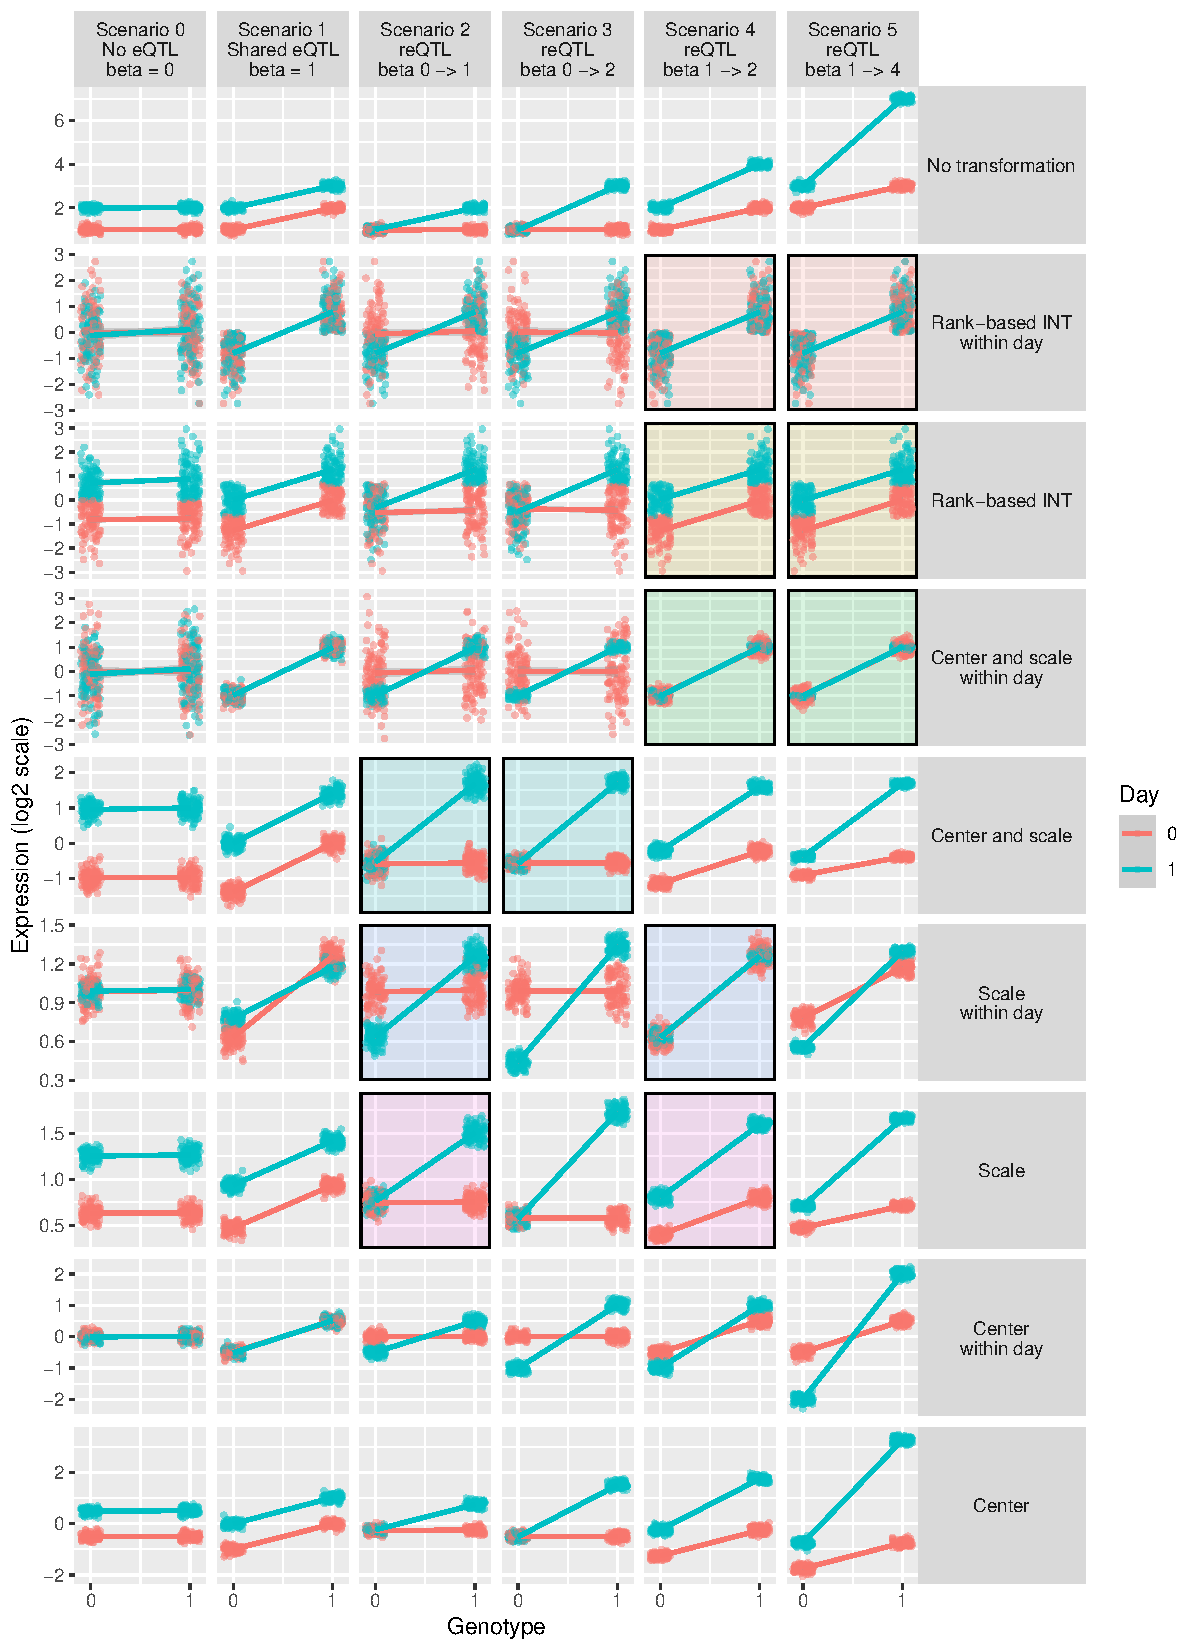
\includegraphics[width=1.0\textwidth,page=1]{mainmatter/figures/chapter_03/simulate_expression_transforms.pdf}
    \caption{
        \textbf{Simulating the effect of data transformation on detection of \gls{reQTL} effects.}
        Expression values on the log scale were simulated for 200 individuals (100 with each genotype) at a baseline and day 1 post-vaccination timepoint.
        Gene expression is upregulated at day 1 by log2FC = 1.
        Six scenarios were simulated with different gene-variant pairs (columns) corresponding to different \gls{eQTL} and/or \gls{reQTL} effects between day 1 and day 0;
        the size of the \gls{reQTL} effect (difference in beta between day 1 and day 0) was set to 0, 0, 1, 2, 1, and 3 for the six scenarios.
        Gaussian noise with mean = 0 and SD = 0.1 was added.
        The top row is the ground truth.
        In following rows, a different transformation is applied within each row, either a rank-based \gls{INT} (Blom offset for fractional ranks \autocite{beasley2009RankBasedInverseNormal,mccaw2020OperatingCharacteristicsRank}), standardising (centering and scaling), centering only, or scaling only;
        Highlighted pairs of scenario-transform combinations on each row represent the induction of false positives or negatives where the size of the relative \gls{reQTL} effects are no longer correct.
    }
    \label{fig:hird_eQTL_expressionTransform_sims}
\end{figure}

\subsection{Genotype phasing and imputation}
\label{subsec:hird_reQTL_methods_genotypePhasingAndImputation}

Genotyping and pre-imputation processing are described in \cref{subsec:hird_dge_genotype_data_generation} and \cref{subsec:hird_dge_genotype_preproc}.
% 2.	Online imputation service to phase and impute chr 1-22 and X
% 2.1.	Phase with Eagle v2.4 (version in imputation logs.tar.gz)
% 2.2.	Impute with PBWT 3.1-v3.1-2-gbf6ebe2+htslib-1.3.2-199-gec1d68e-dirty (version in vcf header)
% 2.2.1.	Reference fa is human_g1k_v37.fasta (1000 genomes)
% 2.2.2.	X chrom is done in 3 chunks
% 2.2.2.1.	X:1-2699520: impute against reference resources/refs/imputation/hrc.r1.1/pbwt/HRC.r1-1.GRCh37.chrX_PAR1.shapeit3.mac5.aa.genotypes
% 2.2.2.2.	X:2699521-154931043: impute against reference resources/refs/imputation/hrc.r1.1/pbwt/HRC.r1-1.GRCh37.chrX_nonPAR.shapeit3.mac5.aa.genotypes
% 2.2.2.3.	X:154931044-155270560: impute against reference resources/refs/imputation/hrc.r1.1/pbwt/HRC.r1-1.GRCh37.chrX_PAR2.shapeit3.mac5.aa.genotypes
Prior to imputation, \num{213277} monomorphic variants that provide no information for imputation were removed.
Variant alleles were aligned such that the reference allele matches the GRCh37 reference, and 358 indels were removed, leaving only \glspl{SNP}.
Imputation for the autosomes and X chromosome was conducted using the Sanger Imputation Service\footnote{\url{https://www.sanger.ac.uk/tool/sanger-imputation-service/}}, 
which involved pre-phasing (separate estimation of haplotypes before imputation to improve imputation speed) with EAGLE2 \autocite{loh2016ReferencebasedPhasingUsinga} (v2.4) 
and imputation with PBWT \autocite{durbin2014EfficientHaplotypeMatching} (v3.1) 
against the Haplotype Reference Consortium (r1.1) panel \autocite{mccarthy2016ReferencePanel64}.
Imputed \glspl{SNP} were lifted-over from GRCh37 to GRCh38 coordinates using CrossMap \autocite{zhao2014CrossMapVersatileTool}.
% 4.	Filtering
% 4.1.	BCFTOOLS_INCLUDE="MAF>$MAF_THRESH & F_MISSING<0.05 & FILTER==\"PASS\" & INFO/INFO>0.4"
% 4.2.	Use MAF thresholds 0.05, 0.10, 0.20
Poorly-imputed \glspl{SNP} with imputation information score $\text{INFO} < 0.4$
% or post-imputation missingness $> 5\%$
were removed, leaving \num{40290981} \glspl{SNP} measured for the 169 genotyped individuals.

\subsection{Estimation of kinship matrices}
\label{subsec:hird_reQTL_LDAK}

% 1.	Build GRM using LDAK 5
% 1.1.	Start with pre-imputed genotypes coreex_eQTLflu_20171204.gencall.smajor.impute_sex.qc6
% 1.1.1.	“Estimates of SNP heritability are very sensitive to genotyping errors”, so we can’t use imputed SNPs without filtering for high INFO.
% 1.2.	Prune to MAF 0.05, autosomes only
% 1.3.	Compute LDAK SNP weightings
% 1.4.	Compute kinships for each chromosome
% 1.5.	Join per-chromosome kinships into genome-wide kinships
% 1.5.1.	Use the leave-one-chromosome-out strategy
%
When testing a variant for association using \glspl{LMM}, to avoid loss of power from \enquote{proximal contamination}, the kinship matrix used should not include that variant \autocite{listgarten2012ImprovedLinearMixed}.
% NOTE: new recommendations to leave out only a small window rather than a chromosome \autocite{widmer2015FurtherImprovementsLinear}
A simple way to avoid this is to compute a \gls{LOCO} kinship matrix using all variants except the ones on the tested variant's chromosome \autocite{lippert2011FaSTLinearMixed}.
I estimated kinship in the \gls{HIRD} data from common autosomal variants, using \software{LDAK} (5.0) \autocite{speed2012ImprovedHeritabilityEstimation}, which computes \glspl{SNP}-based kinship matrices, weighting \glspl{SNP} by \gls{LD} and accounting for genotype uncertainty.
Filtered, pre-imputation sample genotypes from \cref{subsec:hird_reQTL_methods_genotypePhasingAndImputation} were pruned to $\text{\gls{MAF}} > 0.05$.
A kinship matrix was computed for each autosome, then combined into a single genome-wide matrix using \software{LDAK -{}-join-kins}.
To obtain a \gls{LOCO} kinship matrix for each autosome, each autosome's kinship matrix was then subtracted from this genome-wide matrix (\software{LDAK -{}-sub-grm}).
% By default, LDAK scales kinships to have mean zero and average diagonal one

\subsection{Estimation of cell type abundance from expression}
\label{subsec:hird_reQTL_xCell}

% Full notes about cell type correction pipeline rationale at 2019-10-30 in log
%
\Gls{PBMC} samples are a mixture of immune cells, and a fixed input of RNA extracted from that mixture is used to estimate expression, 
so estimates for genes that have cell type-specific expression depend on the relative abundances of each cell type in each sample.
\textcite{sobolev2016AdjuvantedInfluenzaH1N1Vaccination} showed these abundances shift after Pandemrix vaccination.
As genotype can be assumed to stay constant, it is valid to compare the effect size of genotype on expression between multiple timepoints to call \glspl{reQTL}, 
but changes in cell type abundance complicate this by modifying both expression (cell type-specific expression), 
and the effect of genotype on expression (cell type-specific \gls{eQTL} effects).
Immune cell abundance also varies naturally between healthy individuals \autocite{brodin2015VariationHumanImmune,brodin2017HumanImmuneSystem}, so it is important to model these effects not only post-vaccination, but also at baseline.

Cell type abundance directly measured via \gls{FACS} were only available for a small subset of \gls{HIRD} individuals (\cref{subsec:hird_dge_studyDesign}), so I computed cell type abundance estimates from the expression data as an alternative.
\textit{In silico} estimates have previously been used as covariates in \gls{eQTL} analyses in bulk samples where cell type-specific effects are expected \autocite{westra2015CellSpecificEQTL,zhernakova2017IdentificationContextdependentExpression,davenport2018DiscoveringVivoCytokineeQTL,kim-hellmuth2020CellTypeSpecific}.
As the estimates are based on the expression of multiple genes, is not entirely circular to use them as covariates in this way for per-gene \gls{eQTL} models.
%
% https://github.com/dviraran/xCell
%
% xCell uses the expression levels ranking and not the actual values, thus
% normalization does not have an effect, however normalizing to gene length is
% required.
%
% Importantly, xCell performs best with heterogenous dataset. Thus it is
% recommended to use all data combined in one run, and not break down to pieces
% (especially not cases and control in different runs).  xCell uses the
% variability among the samples for the linear transformation. xCell will only
% function with heterogenous mixtures. If there is no variability between the
% samples, xCell will not identify any signal. As noted above, it is highly
% recommended to use all data combined in one run. Failing to do so will again
% inevitably make xCell's results false.
%
% xCell produces enrichment scores, not percentages. It is not a deconvolution
% method, but an enrichment method. That means that the main usage is for
% comparing across samples, not across cell types. xCell does an attempt to make
% the scores resemble percentages, but it is a hard problem, and is very platform
% and experiment specific. We have made some tests to compare the ability of
% xCell for cross-cell types analysis, and found that it generally performed
% better in that than other methods (on limited and comparable cell types), but
% this type of analysis should be performed carefully.  Regarding this issue,
% scaling the scores by samples is extremely dangerous and will inevitably will
% result in false interpretations.
I selected \software{xCell} \autocite{aran2017XCellDigitallyPortraying}, which previously was shown to outperform other deconvolution methods for cell type-specific \gls{eQTL} mapping in blood \autocite{kim-hellmuth2020CellTypeSpecific}.
\software{xCell} computes enrichment scores based on the expression ranks of approximately \num{10000} signature genes derived from purified cell types,
works for both array and \gls{RNAseq} expression data,
and implements \enquote{spillover compensation} to reduce dependency of estimates between related cell types \autocite{aran2017XCellDigitallyPortraying}.
%
% The spillover compensation step may over compensate, thus it is always better
% to run xCell with a list of cell types that are expected to be in the mixture.
% The names of cell types in this list must be a subset of the cell types that
% are inferred by xCell.
%
\software{xCell} was originally developed for tumour samples, so many of the built-in cell types are not expected to be in \gls{PBMC}.
% See 2019-11-14 log
Reviewing the literature to find which broad classes of peripheral blood cell types are commonly-expected in the \gls{PBMC} compartment \autocite{kleiveland2015PeripheralBloodMononuclear,vanderwijst2018SinglecellRNASequencing,davenport2018DiscoveringVivoCytokineeQTL},
I selected 7/64 of the built-in cell types: CD4\textsuperscript{+} T cells, CD8\textsuperscript{+} T cells, B cells, plasma cells, \gls{NK} cells, monocytes, and \glspl{DC}.
% /nfs/users/nfs_b/bb9/workspace/phd/output/hird/rnaseq/4_de/array/array_data_setup.y.filtered.MaxMean.combat.rds
% and /nfs/users/nfs_b/bb9/workspace/phd/output/hird/rnaseq/4_de/array/array_data_setup.sample.metadata.merged.rds
Array and \gls{RNAseq} data from \cref{subsec:hird_dge_array_preproc} and \cref{subsec:hird_dge_rnaseq_quantAndFilter} were processed through \software{xCell} separately, as different internal parameters are used for each platform.
The large batch effect present in the array expression was first removed using ComBat \autocite{johnson2007AdjustingBatchEffects}.
Finally, enrichment scores were standardised across timepoints, so that a score of zero estimates the average abundance of that cell type across all timepoints.
% (\cref{fig:hird_xCell_scores_heatmap_array} and \cref{fig:hird_xCell_scores_heatmap_rnaseq}).

% \begin{figure}
%     \centering
%     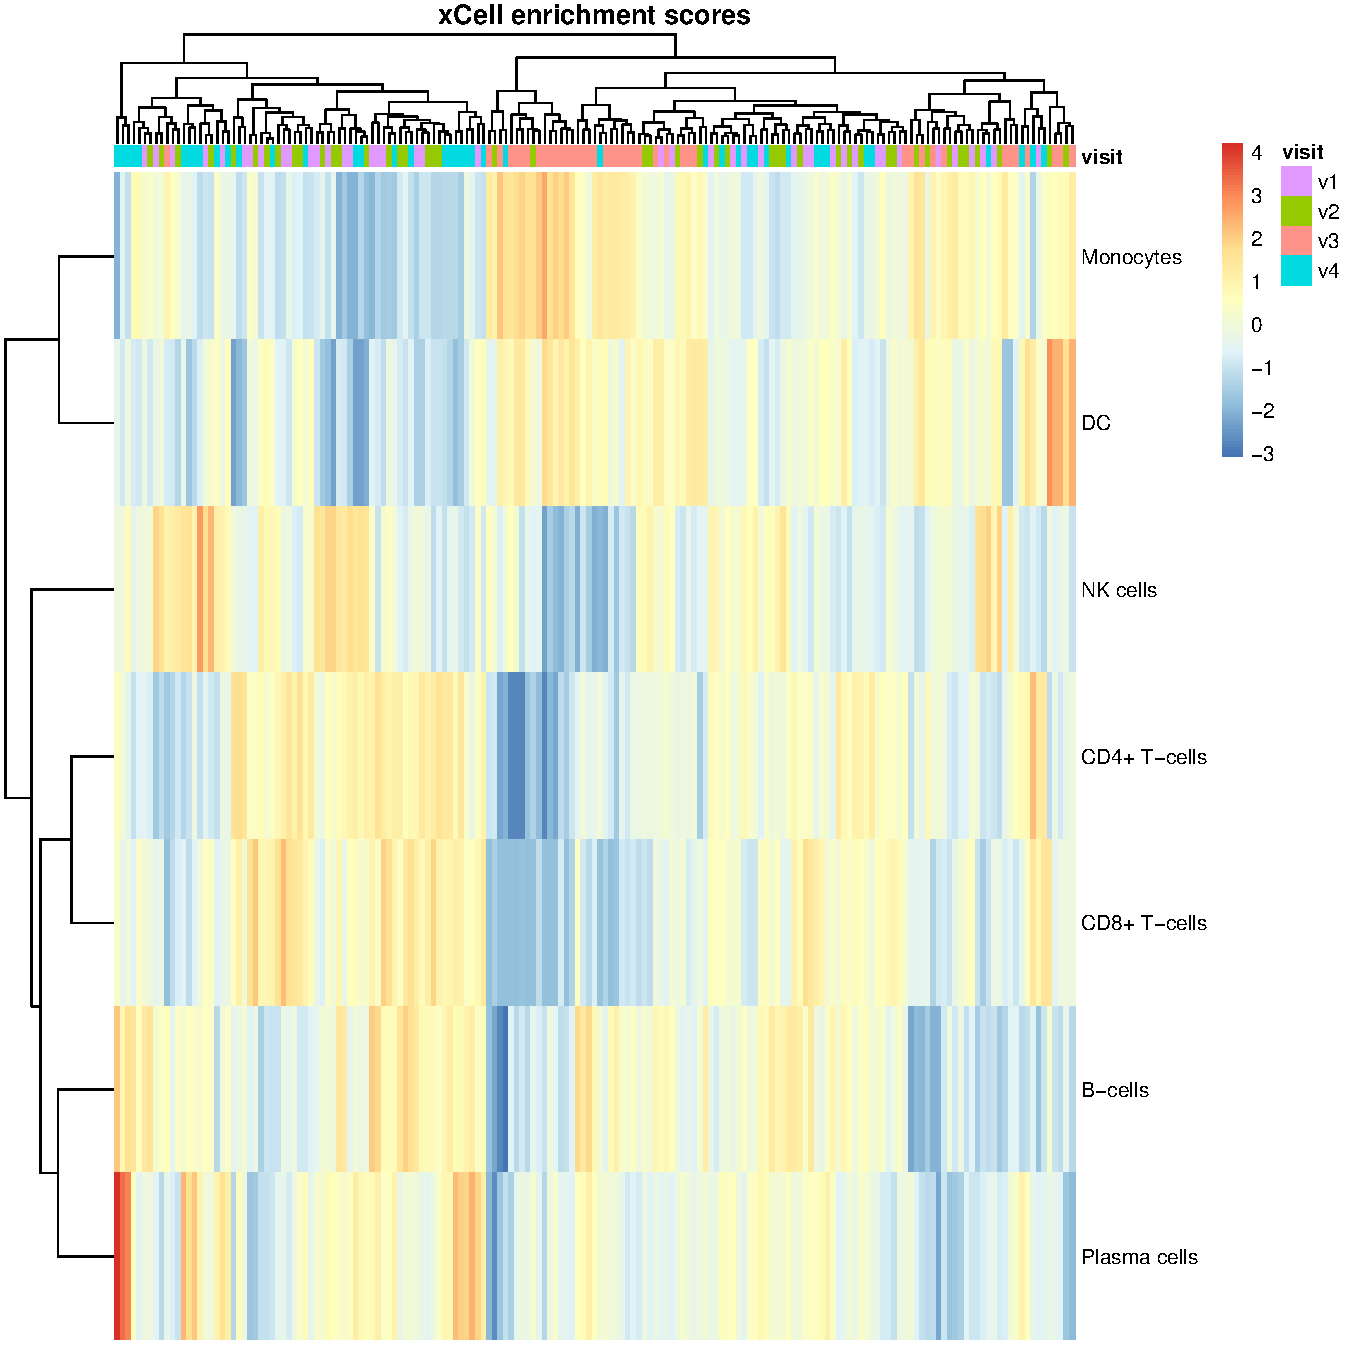
\includegraphics[width=1.0\textwidth,page=1]{mainmatter/figures/chapter_03/get_xCell_estimates.dataset_array.plots.pdf}
%     \caption{Standardised xCell enrichment scores for seven \gls{PBMC} cell types in array samples.}
%     \label{fig:hird_xCell_scores_heatmap_array}
% \end{figure}
%
% \begin{figure}
%     \centering
%     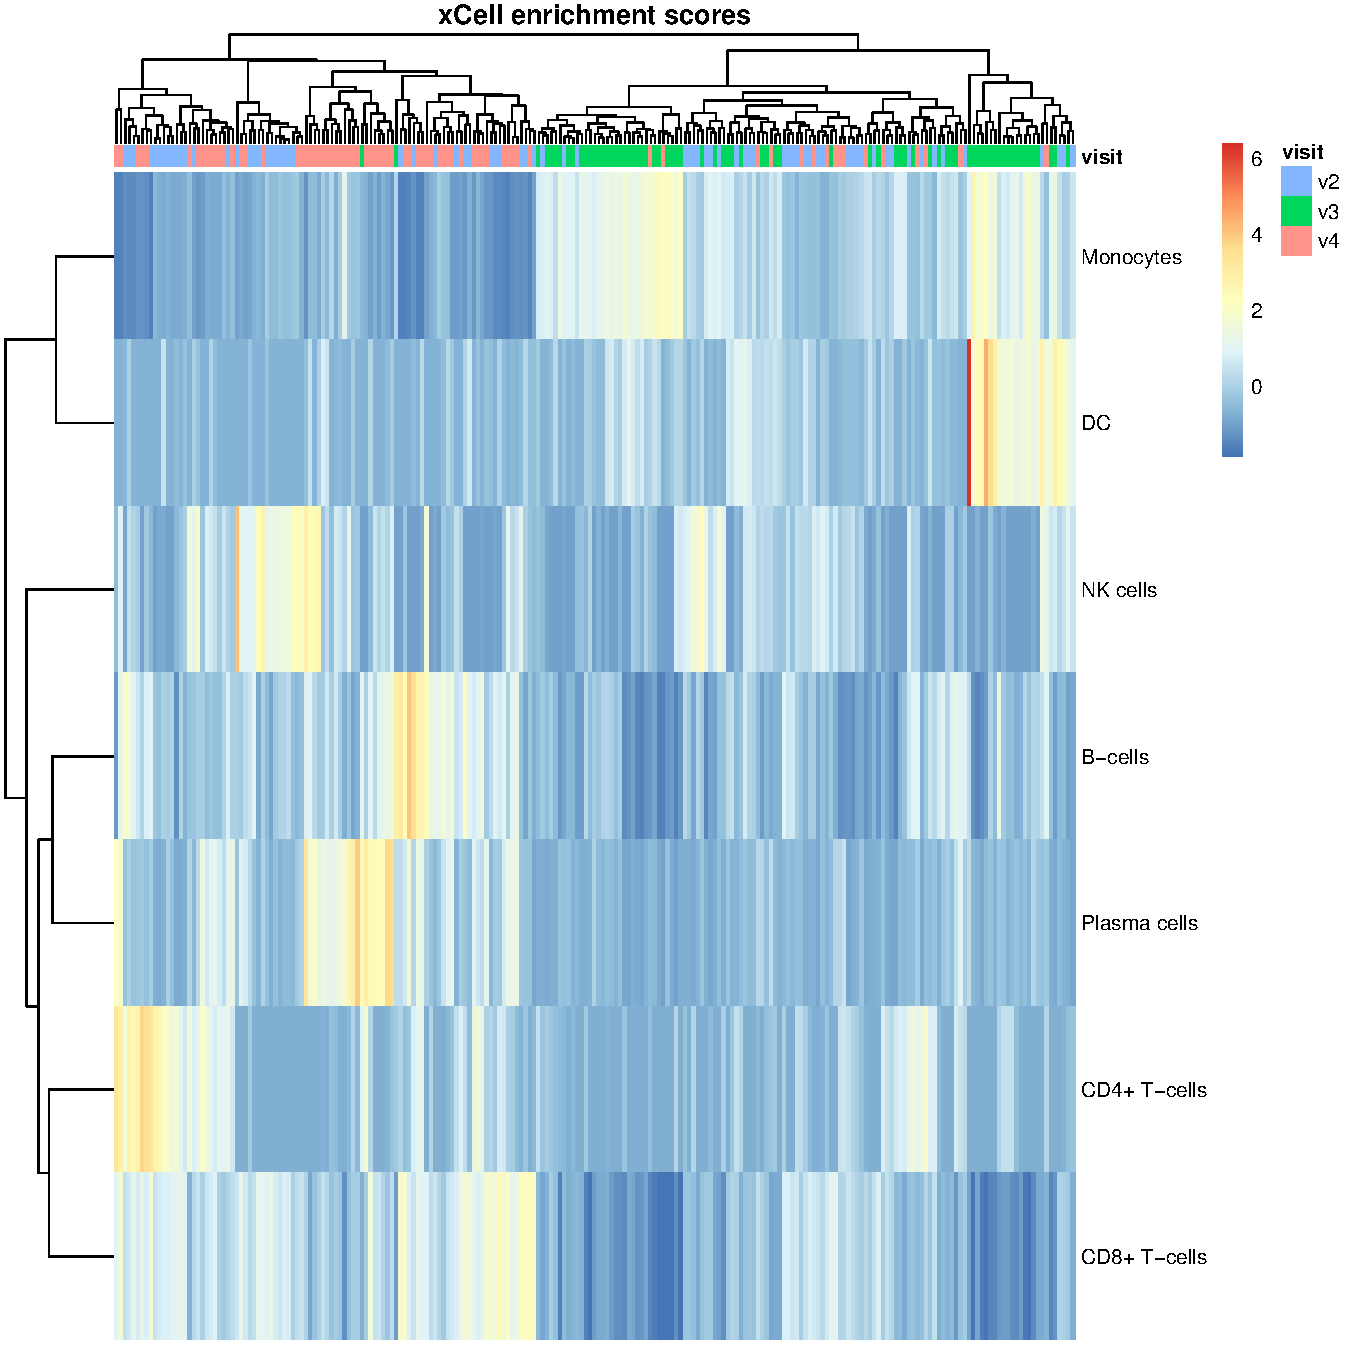
\includegraphics[width=1.0\textwidth,page=1]{mainmatter/figures/chapter_03/get_xCell_estimates.dataset_rnaseq.plots.pdf}
%     \caption{Standardised xCell enrichment scores for seven \gls{PBMC} cell types in \gls{RNAseq} samples.}
%     \label{fig:hird_xCell_scores_heatmap_rnaseq}
% \end{figure}

% xcell estimates not proportions but enrichment scores
As with actual cell type abundances, the enrichment scores are correlated (\cref{fig:hird_xCell_correlationMatrix}).
% NOTE: multicollinearity does not bias the coefficents, but inflates standard errors
Imprecise coefficient estimates due to multicollinearity may be a problem when these scores are used as independent variables in the \gls{eQTL} models% 
\footnote{
    High correlation between predictors is not necessary nor sufficient by itself to induce multicollinearity (predictors being linearly-related), but multiple correlation (how well predictors can be predicted as linear combinations of other predictors) does have an inverse relationship with the standard error of coefficient estimates \autocite{maddala1992IntroductionEconometrics}
}.
% Also see:
% https://stats.stackexchange.com/questions/27300/using-principal-component-analysis-pca-for-feature-selection/27310#27310
To select a subset of cell type scores, I performed a \gls{PCA} of the cell type scores,
separately in array and \gls{RNAseq} datasets (to prevent axes reflecting platform rather than cell type),
% Kaiser Rule
% The more variables that load onto a particular component (i.e., have a high
% correlation with the component), the more important the factor is in
% summarizing the data. An eigenvalue is an index that indicates how good a
% component is as a summary of the data. An eigenvalue of 1.0 means that the
% factor contains the same amount of information as a single variable. [note 1]
the determined the number of \glspl{PC} that exceeded the eigenvalues-greater-than-one rule of thumb \autocite{kanyongo2005InfluenceReliabilityFour}.
In both array and \gls{RNAseq} datasets, the number of components retained was three
The cumulative percentage of variance explained by the top three \glspl{PC} was \SI{81.015345329287}{\percent} and \SI{74.5802450417837}{\percent} in array and \gls{RNAseq} respectively.
Since the \glspl{PC} between the array and \gls{RNAseq} are not directly comparable,
I selected three cell types with high contributions to the top three \glspl{PC} in both datasets:
monocytes, \gls{NK} cells, and plasma cells (\cref{fig:hird_xCell_cos2}).
\textcite{sobolev2016AdjuvantedInfluenzaH1N1Vaccination} reported monocytes and plasma cells to be the cell types with the highest abundance increases at days 1 and 7 respectively.
% The choice to use the actual cell type scores over fitting \glspl{PC} directly as covariates was a sacrifice of orthogonality for interpretability.
Using the actual cell type scores over fitting \glspl{PC} as covariates also provides more interpretable regression coefficients for those terms.

\begin{figure}
    \centering
    \begin{subfigure}[b]{0.65\textwidth}
        \centering
        \includegraphics[width=1.0\textwidth,page=3]{mainmatter/figures/chapter_03/get_xCell_estimates.dataset_array.plots.pdf}
    \end{subfigure}
    \bigskip\vfill
    \begin{subfigure}[b]{0.65\textwidth}
        \centering
        \includegraphics[width=1.0\textwidth,page=3]{mainmatter/figures/chapter_03/get_xCell_estimates.dataset_rnaseq.plots.pdf}
    \end{subfigure}
    \caption{
        \textbf{Correlation matrix of standarised xCell cell type enrichment scores in each dataset.}
        Rows and columns are hierarchically-clustered.
    }
    \label{fig:hird_xCell_correlationMatrix}
\end{figure}

% See:
% https://stats.stackexchange.com/questions/119746/what-is-the-proper-association-measure-of-a-variable-with-a-pca-component-on-a
%
% https://stats.stackexchange.com/questions/495342/pca-and-variable-contributions-to-first-n-dimensions
% If you have a "PCA" object constructed using FactoMineR::PCA, then variable contribution values are stored in the $var$contrib slot of your object. The contribution is a scaled version of the squared correlation between variables and component axes (or the cosine, from a geometrical point of view)
%
% var$contrib: contains the contributions (in percentage) of the variables to the
% principal components. The contribution of a variable (var) to a given principal
% component is (in percentage) : (var.cos2 * 100) / (total cos2 of the
% component).
\begin{figure}
    \centering
    \begin{subfigure}[b]{0.65\textwidth}
        \centering
        \includegraphics[width=1.0\textwidth,page=10]{mainmatter/figures/chapter_03/get_xCell_estimates.dataset_array.plots.pdf}
    \end{subfigure}
    \bigskip\vfill
    \begin{subfigure}[b]{0.65\textwidth}
        \centering
        \includegraphics[width=1.0\textwidth,page=10]{mainmatter/figures/chapter_03/get_xCell_estimates.dataset_rnaseq.plots.pdf}
    \end{subfigure}
    \caption{
        \textbf{
            Contribution of each cell type score to each \gls{PC} dimension after \gls{PCA} of standarised xCell cell type enrichment scores. 
        }
        Contribution is calculated as the squared correlation between a variable and a \gls{PC} (cos2), 
        scaled to the sum of cos2 for all variables with \gls{PC}.
        High contributions indicate variables that are correlated with the \gls{PC}.
    }
    \label{fig:hird_xCell_cos2}
\end{figure}

Scores were validated against \gls{FACS} measurements from \textcite{sobolev2016AdjuvantedInfluenzaH1N1Vaccination} in the subset of \textapprox{40} individuals that had both expression and \gls{FACS} data.
Depending on each \gls{FACS} panel's gating strategy for each cell subset, the data were in units of either absolute counts, or percentage of the previously gated population.
Values were normalised by rank-based \gls{INT} within each panel and cell subset (\autocite{astle2016AllelicLandscapeHuman} takes a similar approach for cell abundance data using a quantile-based \gls{INT}).
% RANK INT also used in phenome scan PHEASANT https://www.biorxiv.org/content/biorxiv/early/2017/02/26/111500.full.pdf
%
% missForest is a nonparametric imputation method for basically any kind of data.
% It can cope with mixed-type of variables, nonlinear relations, complex
% interactions and high dimensionality(p>>n). It only requires the observation
% (i.e. the rows of the data frame supplied to the function) to be pairwise independent.
Missing values were then imputed with MissForest \autocite{stekhoven2012MissForestNonparametricMissing}, a random forest imputation method suitable for high-dimensional mixed-type data where $p \gg n$.
An initial guess for missing values is established using mean- or mode-imputation, then a random forest is trained on the observed part of the data and used to predict and update the values of the missing part.
The process repeats iteratively until convergence.
% NOTE:
% Why impute for cell counts but not for expression data?
% - expression matrices are mostly complete, and we only exclude genes based on low expression in RNAseq
% - we cannot drop whole FACS panels so easily like we can drop genes

Although the increases in xCell score for monocytes at day 1 and plasma cells at day 7 do reflect the increases in these cell types observed by \textcite{sobolev2016AdjuvantedInfluenzaH1N1Vaccination}, overall correlation between xCell and \gls{FACS} was poor (\cref{fig:hird_xCell_vs_FACS}).
Substantial discrepancy was expected, as the cell types as defined in the xCell signatures do not directly correspond to the combinations of surface markers used for \gls{FACS}; the comparison is against the closest match.
The \gls{FACS} gating strategy also meant that for some cell populations, the only available \gls{FACS} measure was a proportion of the previously gated population,
whereas xCell attempts to estimate scores that represent enrichments in the whole mixture.
The accuracy of the built-in signatures may also be lower when applied to the expression matrix for a stimulated state,
and an enrichment-based method can not distinguish per-cell differential expression of signature genes from changes in cell abundance.
A custom signature matrix can be used for xCell, perhaps drawn from an independent study with similar stimulation conditions as \gls{HIRD} such as \textcite{franco2013IntegrativeGenomicAnalysis}, but this would not solve the issue of coupled differential expression and cell abundance.
Weighing the downsides of having imperfect estimates of cell type abundance against the downsides of not accounting for abundance, or excluding samples without \gls{FACS} measures, I chose to continue the analysis using the xCell scores.
These scores can distinguish large changes in cell abundances between days, but may not be reliable for distinguishing small differences in abundance between individuals with a timepoint. 

\begin{figure}
    \centering
    \begin{subfigure}[b]{0.43\textwidth}
        \centering
        \includegraphics[width=1.0\textwidth,page=6]{mainmatter/figures/chapter_03/validate_xCell_estimates.cell_type_pairs.pdf}
        \caption{Monocytes.}
    \end{subfigure}
    \bigskip\vfill
    \begin{subfigure}[b]{0.43\textwidth}
        \centering
        \includegraphics[width=1.0\textwidth,page=3]{mainmatter/figures/chapter_03/validate_xCell_estimates.cell_type_pairs.pdf}
        \caption{\gls{NK} cells.}
    \end{subfigure}
    \bigskip\vfill
    \begin{subfigure}[b]{0.43\textwidth}
        \centering
        \includegraphics[width=1.0\textwidth,page=2]{mainmatter/figures/chapter_03/validate_xCell_estimates.cell_type_pairs.pdf}
        \caption{Plasma cells.}
    \end{subfigure}
    \caption{
        \textbf{Comparison of standardised xCell scores for monocytes, \gls{NK} cells and plasma cells with normalised \gls{HIRD} \gls{FACS} measurements.}
        The comparisons are against the most comparable measurements from the \gls{FACS} data of \textcite{sobolev2016AdjuvantedInfluenzaH1N1Vaccination}: 
        CD14+ monocyte count,
        CD56+ NK cells count,
        and the proportion of CD19+ B cells that were CD19+CD27+CD24hiCD38hi plasma cells.
        Missing \gls{FACS} values were imputed with MissForest after rank-based \gls{INT} transformation.
    }
    \label{fig:hird_xCell_vs_FACS}
\end{figure}

\subsection{Finding unmeasured covariates using factor analysis}
\label{subsec:hird_reQTL_PEER}

% If RANKINT, why RANKINT before PEER?
%
% Are your covariates under control? How normalization can re-introduce covariate effects
% https://www.ncbi.nlm.nih.gov/pubmed/29706643
% "Many statistical tests rely on the assumption that the residuals of a model are normally distributed [1]. In genetic analyses of complex traits, the normality of residuals is largely determined by the normality of the dependent variable (phenotype) due to the very small effect size of individual genetic variants [2]. However, many traits do not follow a normal distribution."
% "applying rank-based INT to the dependent variable residuals after regressing out covariates re-introduces a linear correlation between the dependent variable and covariates, increasing type-I errors and reducing power."

% 2.	Infer global confounders by detecting hidden factors affecting expression with PEER
% 2.1.	“batch effects and other global confounders reduce the power to find expression quantitative trait loci”
% 2.1.1.	“We assume that these variables have a broad influence, and thus each of them has an effect size for every gene.”
% 2.1.2.	“The learned variables can be constrained to affect known sets of genes via a prior connectivity matrix. By default, with no prior connectivity given, they are assumed to be global and to affect large fractions of all genes“
% 2.1.3.	Note that due to this assumption: “If large trans hotspots are dominating, associations may get erroneously explained away as confounding factors”
% 2.2.	Round input expression to integer counts
% 2.2.1.	Input is y: the scaledTPM (TPM's scaled up to library size) from tximport.
% 2.3.	Normalise for library size and variance stabilize with varianceStabilizingTransformation from DESeq2 (recommended in PEER paper)
% 2.3.1.	Vst is like a souped up log: “In all cases, the transformation is scaled such that for large counts, it becomes asymptotically (for large values) equal to the logarithm to base 2 of normalized counts.”
% 2.3.2.	Note we cannot use voom-ed expressions from the DGE pipeline, as there are some samples missing due to lack of Ab titre data
% 2.3.3.	Do not blind the transformation to experimental design matrix: “If many of genes have large differences in counts due to the experimental design, it is important to set blind=FALSE for downstream analysis.”
% 2.3.4.	Here we use a simple design matrix of groups defined by all combos of day x R/NR
% 2.4.	Run PEER by timepoint
% 2.4.1.	Match GTeX pipeline: https://github.com/broadinstitute/gtex-pipeline/tree/63b13b8ced25cf8ab8e7a26f40a495e523630a9b/qtl , with some modifications.
% 2.4.1.1.	Note this pipeline uses quantile normalized, rank INT transformed expression, as PEER input
% 2.4.2.	Quantile normalize the samples with preprocessCore::normalize.quantiles
% 2.4.2.1.	Causes the expressions of the samples to have the same empirical distribution
% 2.4.2.2.	i.e. the the highest expression in each sample is set to the mean of the highest values of all samples, and in the case of no tied values, each sample’s expressions becomes a permutation of each other sample’s
% 2.4.3.	Standardize expression of each gene with Rank-Based Inverse Normal Transformation
% 2.4.3.1.	i.e. rank the expressions of a gene, then replace with values from the standard normal e.g. > rank.based.INT(1:5, c=3/8): [1] -1.1797611 -0.4972006  0.0000000  0.4972006  1.1797611
% 2.4.4.	Setup and run PEER
% 2.4.4.1.	Allow up to 10k iterations, start with n.samples/4 PEER factors
% 2.4.4.2.	One can include known covariates. We don’t, as it causes weird things like PEER factors not being sorted in descending relevance
% 2.4.4.2.1.	~ 1 + batch + rna.conc + Gender + Age.at.vaccination..years. + PC1.imputed + PC2.imputed + PC3.imputed + PC4.imputed
% 2.4.4.2.2.	Note this includes an intercept that represents the mean expression
%
% Also interesting:
% PANAMA/LIMMI, by PEER authors
% Detecting regulatory gene–environment interactions with unmeasured environmental factors
%
Apart from cell type abundance, a myriad of other unmeasured variables contribute to expression variation.
Hidden determinants of expression variation were learnt using \software{PEER} \autocite{stegle2012UsingProbabilisticEstimation}.
As suggested by \textcite{stegle2012UsingProbabilisticEstimation}, I used \software{DESeq2::vst} to perform between-sample normalisation and variance stabilisation on \gls{RNAseq} count data%
\footnote{
    The count data were taken from \cref{subsec:hird_dge_rnaseq_quantAndFilter} before \gls{TMM} normalisation and voom transformation,
    as PEER cannot use the weights output by those methods for between-sample normalisation and variance stabilisation as limma can.
}.
ComBat was applied to first merge array and \gls{RNAseq} data into a single log scale expression matrix per timepoint, treating the largest global effects on expression---the two array batches and three \gls{RNAseq} library prep pools (\cref{fig:hird_expression_pcs})---as known batch effects.
% (e.g., by introducing principal components of the genotype data), is not included in the model, and it may be recapitulated in the inferred factors.
Given a set of known covariates (intercept, sex, four genotype \glspl{PC} from \cref{subsec:hird_dge_genotype_pc} representing ancestry, and the three xCell scores estimated above),
PEER was used to estimate additional hidden factors that explain variation in the expression matrix,
which can be technical (e.g. sample quality/concentration, library preparation plate/reagents, processing time, lane/flow cell)
or biological (e.g. cell type composition, ancestry).
Factors are assumed to be unmeasured covariates that have global effects on a large fraction of genes, 
whereas a cis-\gls{eQTL} will typically only have local effects, so including factors as covariates should not introduce dependence with the genotype term,
but should explain some of the residual variation, improving power to detect cis-\glspl{eQTL}.
% This is also the primary motivation behind recommendation of including prognostic covariates in RCTs \url{https://trialsjournal.biomedcentral.com/articles/10.1186/1745-6215-15-139}
The analysis was run per timepoint, otherwise global changes in expression between timepoints induced by the vaccine would be recapitulated as factors.

Correlating the estimated factors to a larger set of known covariates reveals many correlations with xCell estimates, indicating that cell type abundance does indeed have substantial global effects on the expression matrix  (\cref{fig:hird_peer_corMatrix_v2_mega}).
These estimated factors likely represent additional cell types with an abundance that has a global effect on the expression matrix,
and when used as covariates in combination with the three major cell type scores selected in \cref{subsec:hird_reQTL_xCell}, should improve overall adjustment for cell composition.
% NOTE: PEER for ancestry
% \autocite{brown2018ExpressionReflectsPopulation}
% Interestingly, we found that using PEER rather than regression for batch correction also removed the separation between the YRI and EUR individuals, while leaving the structure within the EUR populations in tact (Fig 5A).
There is little correlation with known array or \gls{RNAseq} batch effects, indicating ComBat did an adequate job of removing batch- and platform-dependent global effects on expression prior to PEER.
Note that I did not leave this adjustment for PEER to perform, as ComBat estimates centering and scaling factors per gene and batch, whereas the use of PEER factors represents a mean-only per-gene adjustment.
Given the severity of the batch effect in this dataset, especially between platforms, mean-only adjustment may be insufficient \autocite{zhang2018AlternativeEmpiricalBayes},
particularly in the context of \textit{cis}-\gls{eQTL} mapping where the variant will only explain a small fraction of expression variance.

\begin{figure}
    \centering
    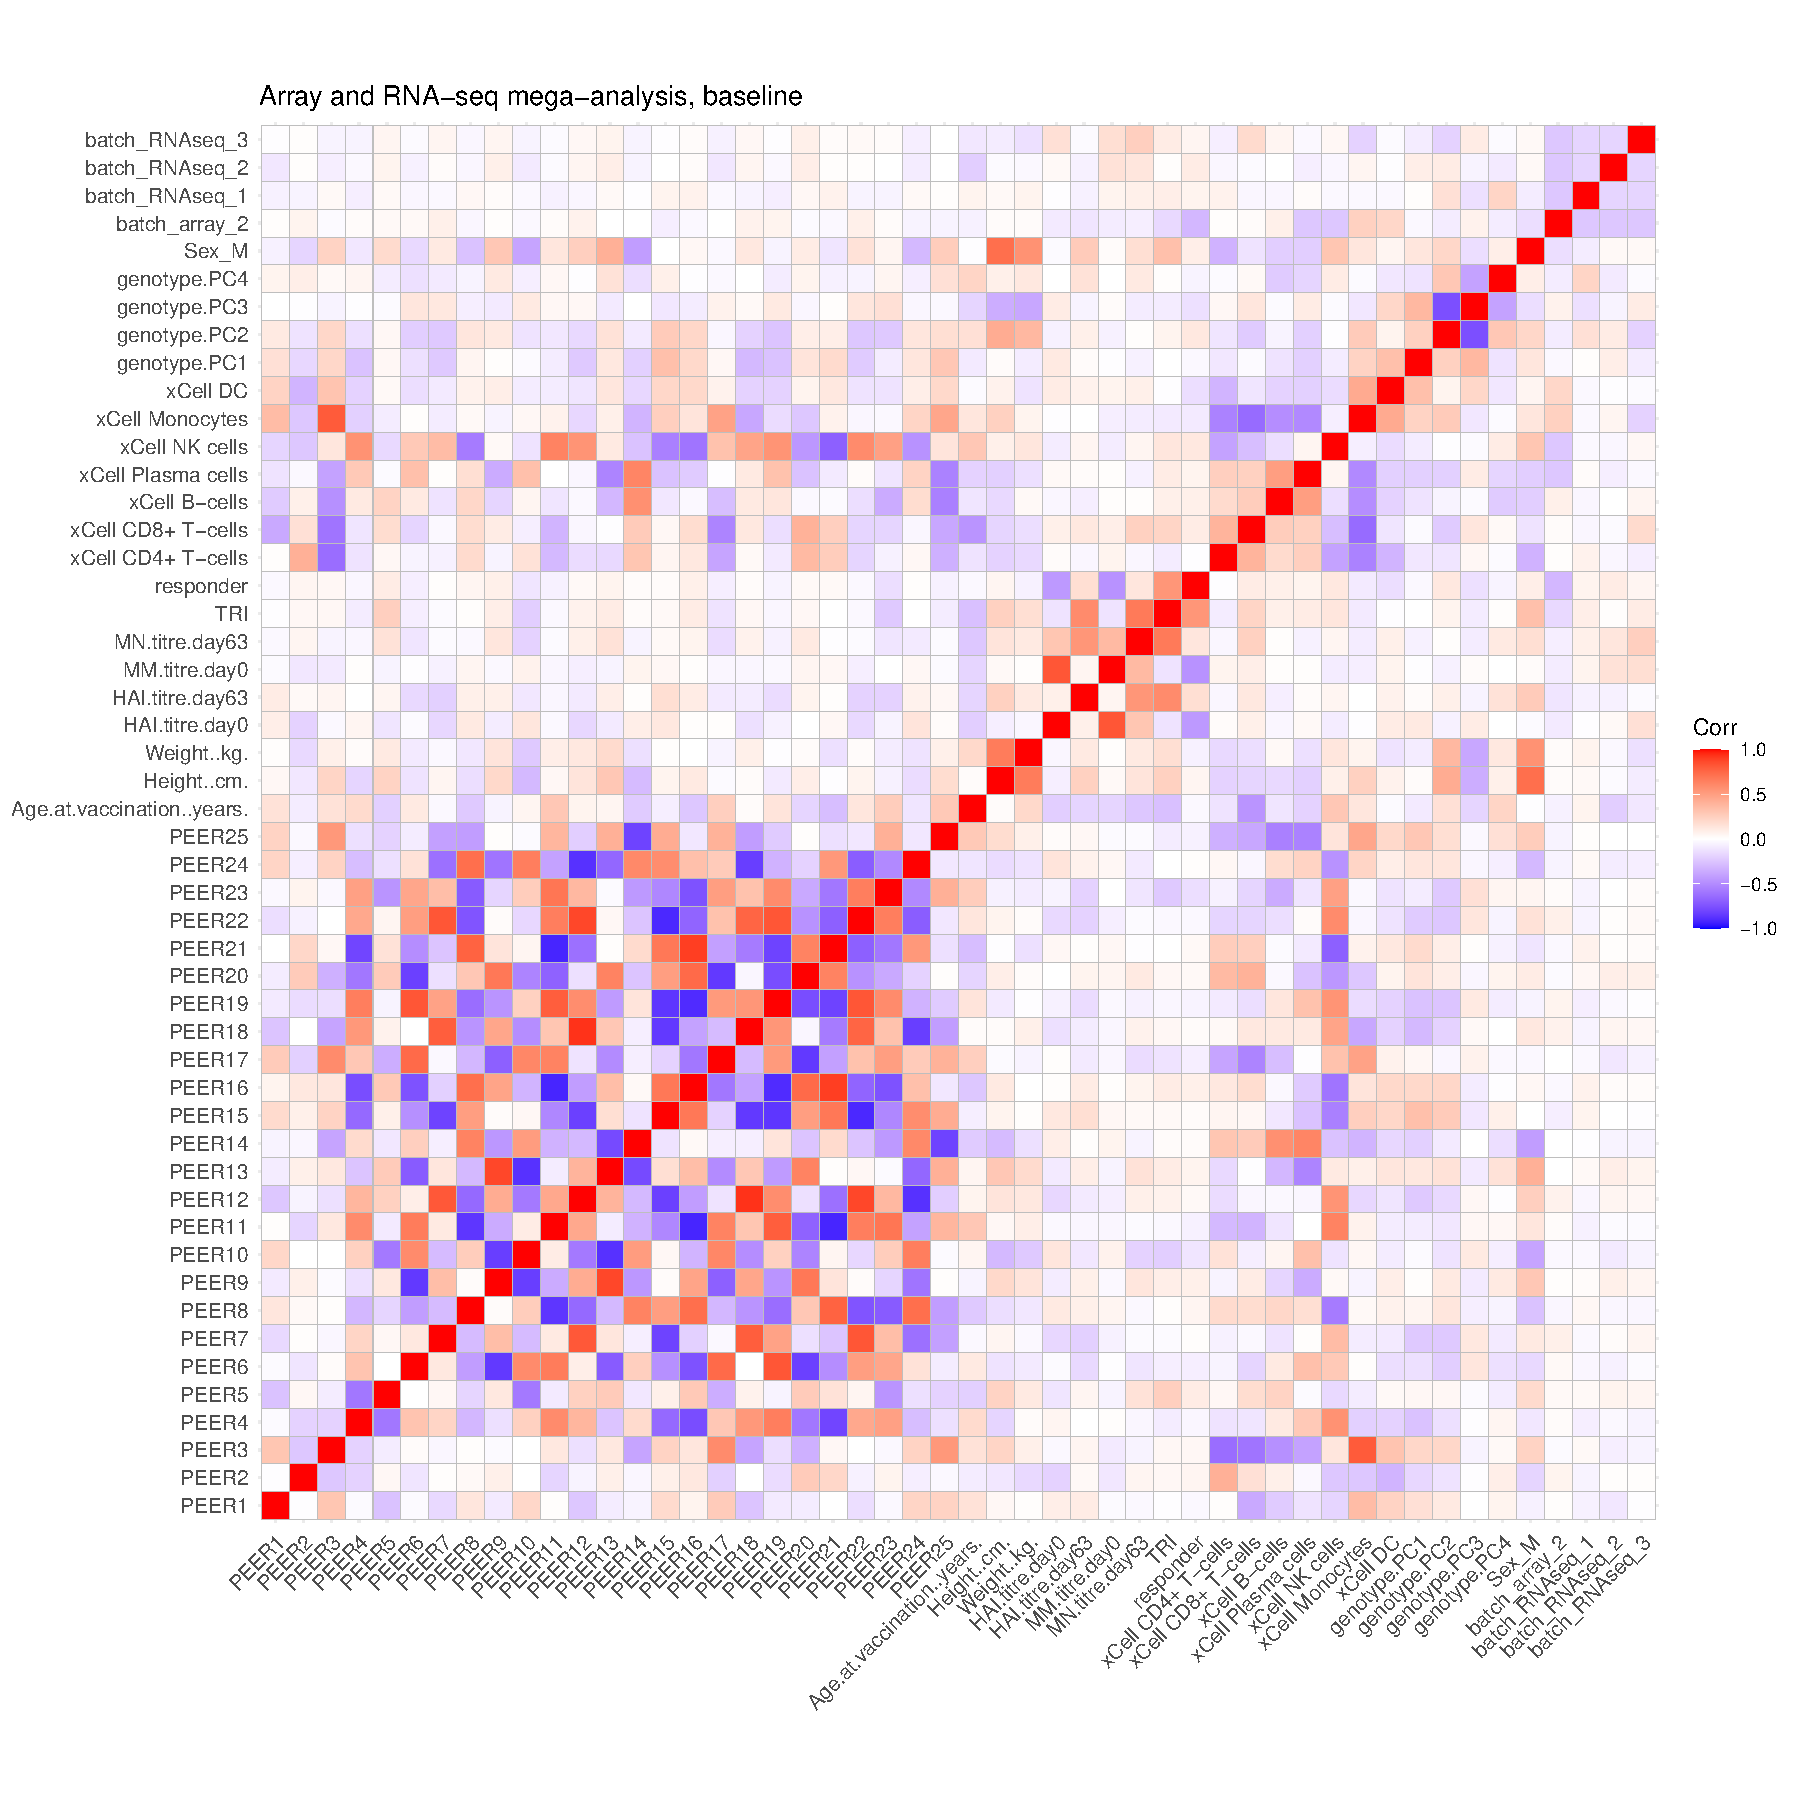
\includegraphics[width=1.0\textwidth,page=1]{mainmatter/figures/chapter_03/peer_plotting.mega_v2.pdf}
    \caption{
        \textbf{Correlation of known variables to the first 25 PEER factors estimated from the array and \gls{RNAseq} mega-analysis expression data at baseline.}
        The known factors provided to PEER were sex, four genotype \glspl{PC}, and monocyte, \gls{NK} cell and plasma cell xCell scores.
        PEER factors are not constrained to be orthogonal like \glspl{PC}, so correlations to known factors and other PEER factors are expected.
        The estimated factors have zero mean, and PEER implements automatic relevance determination \autocite{stegle2012UsingProbabilisticEstimation}, which decreases the variance of successive estimated factors to zero if they no longer explain additional expression variance.
        There are extensive correlations between higher numbered factors,
        but these factors have near-zero variance.
        % NOTE: no guarantee of decreasing variance ordering of PEER factors when known factors are given
    }
    \label{fig:hird_peer_corMatrix_v2_mega}
\end{figure}

\subsection{\glsfmtshort{eQTL} mapping per timepoint}
\label{subsec:hird_reQTL_limix}

% 2.5.	Preprocess genotypes for limix
% 2.5.1.	Convert MAF filtered VCF -> 012 -> hdf5 format
% 2.5.1.1.	Do this for both strict 012 and continuous dosages
% 2.5.2.	Also convert 012 -> matrix eqtl SNP matrix format
% 2.5.2.1.	For eigenMT
% 2.5.3.	Parse out snpinfo and snplocs from VCFs
% 2.5.3.1.	Snpinfo for snp ids, for limix
% 2.5.3.2.	Snplocs for snp positions, and eigenMT
% 2.6.	Map eQTLs using limix 2.0, per timepoint
% 2.6.1.	Map cis-eQTLs within +- 1Mb of the gene start
% 2.6.1.1.	Phenotypes: per timepoint normalised input.expr from PEER script
% 2.6.1.2.	Covariates: sex, batch, 4 genotype PCs, 4 PEER factors
% 2.6.1.3.	Genotypes: MAF > 0.10 (in whole 169 individuals)
% 2.6.1.4.	Kinship: from LDAK, leave-one-chrom-out
% 2.6.2.	Output results in matrix eqtl-like output format
%
I mapped \glspl{eQTL} within each timepoint using \software{LIMIX} \autocite{lippert2014LIMIXGeneticAnalysis}, which implements univariate and multivariate \glspl{LMM} with one or more random effects.
Imputed genotype probabilities were converted to continuous alternate allele dosages using bcftools (1.7-1-ge07034a).
Variants with sample $\text{\gls{AC}} < 15$ of the minor allele within each timepoint were excluded, 
corresponding to a \SIrange{5}{7}{\percent} \gls{MAF} depending on timepoint.
% NOTE: AN day 0 290 day 1 210 day 7 214
At the sample size of \gls{HIRD}, \gls{FDR} cannot be controlled by standard hierarchical \gls{FDR} methods without a \gls{MAF} filter of approximately \SIrange{5}{10}{\percent} \autocite{huang2018PowerFalseDiscovery}.

% NOTE: this includes X chromosome genes
At each of \num{13570} genes, at all cis-variants within within $\pm \SI{1}{\mega\bp}$ of the gene \gls{TSS}, I fit the following model to map \gls{eQTL}:
% NOTE: used Ensembl GENESEQSTART if fwd strand, otherwise GENESEQEND
% Like all Ensembl features the start of an exon is always less than or equal to the end of the exon, regardless of the strand it is on. The start of the transcript is the start of the first exon of a transcript on the forward strand or the end of the last exon of a transcript on the reverse strand. The start and end of a gene are defined to be the lowest start value of its transcripts and the highest end value respectively.
\begin{equation}
    \begin{split}
    Y = 1 + sex + \sum_{i=1}^{4}{PC_i} + \sum_{}^{3}{xCell} + \sum_{i=1}^{k}{PEER_i} + \beta G + \mathbf{u} + \epsilon
    \end{split}
    \label{eq:hird_reQTL_limix_model}
\end{equation}
% TODO: check mathbf for vector notation, add timepoint subscript
where the \gls{eQTL} effect size of interest is the slope of the genotype fixed effect $\beta$, the average additive effect of the alternate allele \autocite{visscher2019Fisher1918Paper};
and $\mathbf{u} \sim N(0, \sigma_g^2 K)$ is a random effect with zero mean and covariance matrix proportional to the \gls{LOCO} kinship matrix.
For chromosome X variants, no \gls{LOCO} matrix is available from LDAK, so the matrix for chromosome 1 was used.
% TODO note stacking of kinship for day -7 repeated measures

PEER factors are automatically weighted such that the variance of factors tends to zero as more factors are estimated, 
hence continuing to add more and more factors as covariates will not continue to improve \gls{eQTL} detection power, and eventually the model degrees of freedom will be depleted.
To optimise the number of factors $k$ to include as covariates%
\footnote{I avoid the commonly-performed two-stage approach of treating PEER residuals as expression phenotypes, as the degrees of freedom seen downstream will be incorrect, which can have a substantial effect on estimates at this modest sample size.}, 
% Also see \autocite{demissie2011BiasDueTwostage} % holmes2019ProblemsInterpretingUsing
per-timepoint \gls{eQTL} mapping was performed in chromosome 1, iteratively increasing the number of factors until including additional factors provides no further benefit, and the number of \glspl{eQTL} detected stabilises.
I settled on a final choice of 10 factors for pre-vaccination, 5 factors for day 1, and 5 factors for day 7 (\cref{fig:hird_neGenesvsPeerK}).

\begin{figure}
    \centering
    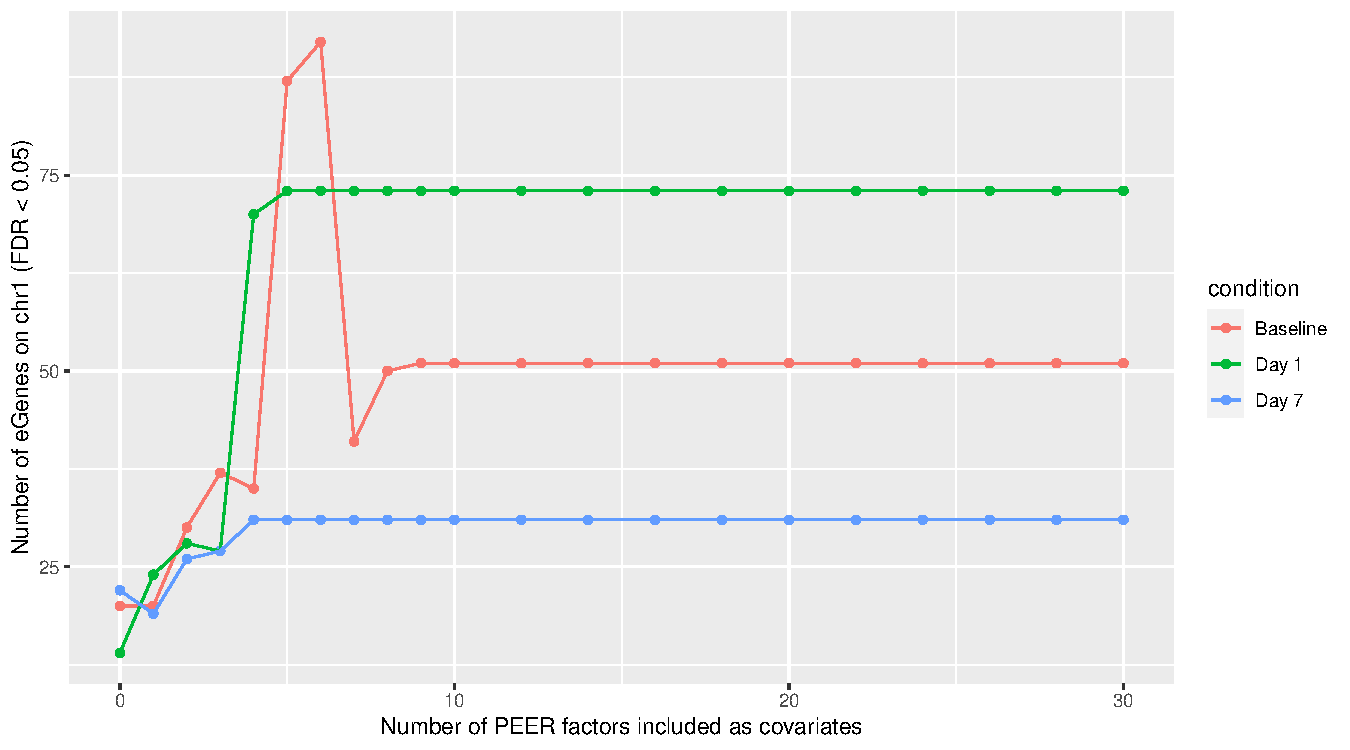
\includegraphics[width=1.0\textwidth,page=1]{mainmatter/figures/chapter_03/count_eGenes.signif_eGenes_vs_PEER_n.dataset_mega.chr_chr1.pdf}
    \caption{
        \textbf{Number of significant genes with an \gls{eQTL} detected on chromosome 1, as a function of the number of PEER factors included as covariates.}
        \gls{FDR} computed with hierarchical Bonferroni-\gls{BH} \autocite{huang2018PowerFalseDiscovery} with significance threshold set at 0.05.
        The number of eGenes stabilises since higher number PEER factors explain less and less variance in expression, so have less and less influence on the regression.
    }
    \label{fig:hird_neGenesvsPeerK}
\end{figure}

\subsection{Joint \glsfmtshort{eQTL} analysis across timepoints}
\label{subsec:hird_reQTL_mashr}

% 2.10.	mashr
% 2.10.1.	Apply mashr to per-day meta-analysis beta/beta_ste results
Joint analysis was conducted with \software{mashr} \autocite{urbut2018FlexibleStatisticalMethods} at \num{40197618} gene-variant pairs (mean of \num[round-mode=places,round-precision=0]{2962.24156227} tests per gene) for which summary statistics from within timepoint mapping were available in all three timepoint conditions.
For $n$ conditions, the mashr model incorporates multiple $n \times n$ canonical and data-driven covariance matrices to represent patterns of effects across conditions.
% NOTE: https://stephenslab.github.io/mashr/reference/cov_canonical.html
Canonical matrices include the identity matrix (representing independent effects between conditions), singleton matrices (effects only in one condition), a matrix of ones (equal effects in all conditions), and other patterns of correlations.
Data-driven covariance matrices represent patterns of effect observed empirically, derived from dimension reduction of a strong subset of tests likely to have an effect in at least one condition.
% NOTE: obviously, the variant could be different in each condition
I took the most significant variant per gene per condition, 
which ensures strong condition-specific effects are included,
% (\cref{fig:hird_mashr_strongSubset_Z_mega}),
then further filtered to only nominally significant tests, resulting in a strong subset of 45962 tests, then used to calculate data-driven covariance matrices.

% \begin{figure}
%     \centering
%     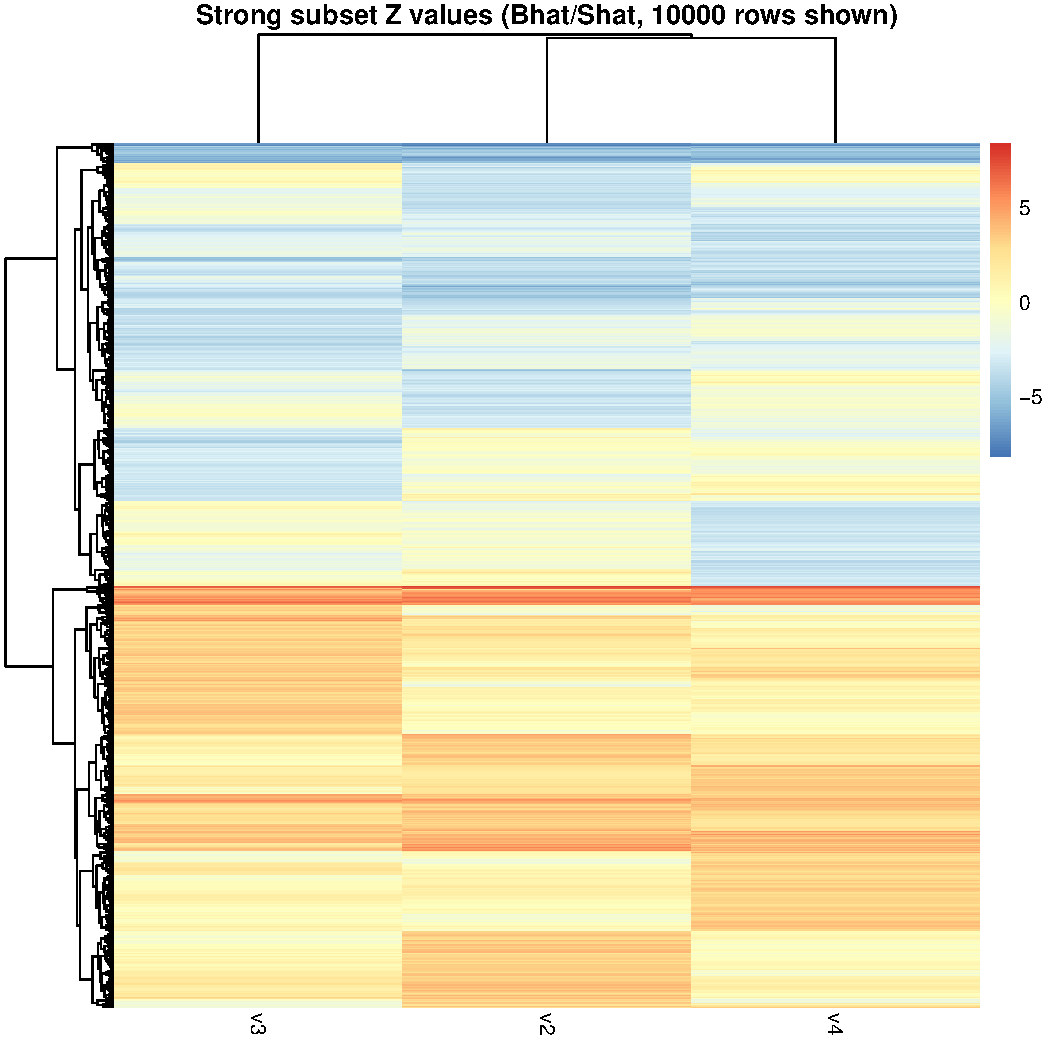
\includegraphics[width=1.0\textwidth,page=1]{mainmatter/figures/chapter_03/mash_mega/mashr.strong_subset_zval_heatmap.cisDist_1e6.sampleAcThresh_15.randomSubsetN_200000.pdf}
%     \caption{Clustering of within-timepoint Z scores in the strong mashr subset (random sample of 10000/45962 tests), confirming the presence of strong condition-specific effects.}
%     \label{fig:hird_mashr_strongSubset_Z_mega}
% \end{figure}

The \software{mashr} model was trained on a random subset of \num{200000} tests, using the Exchangeable Z-scores model (assumes effects are independent of their standard errors, which performed better in GTEx data \autocite{urbut2018FlexibleStatisticalMethods}).
% An alternative is to allow the effects to scale with standard error, so that effects with larger standard error tend to be larger.
The correlation of null tests between conditions---critical to account for due to the repeated measures structure of the data---was estimated using \software{mashr::estimate\_null\_correlation}, which uses tests from the random subset that have small $z$-scores.
The fitted model was used as a prior to compute posterior effects and standard errors for all tests through shrinkage.
A condition-specific Bayesian measure of significance \gls{lfsr} is returned, 
the probability that the declared sign of the effect is incorrect \autocite{stephens2016FalseDiscoveryRates}.
Note that \software{mashr} is the multiple-condition extension of \software{ashr}, 
previously used in \cref{subsubsec:hird_dge_multipleTestingCorrection} for computing posterior effects and their significance in \gls{DGE} analyses.

\subsection{Defining shared and response eQTLs}
\label{subsec:hird_reQTL_methods_definingSharedAndreQTLs}

Many of the tested variants for each gene will be in high \gls{LD}.
% qtls.merged[, signif_rank := frank(qtls.merged, lfsr, -INFO, -MAF_sample, SNP_gene_TSS_dist, POS)]
To unambiguously select a lead \gls{eQTL} variant per gene for comparison across timepoints, I selected the variant with the lowest lfsr over all conditions.
If multiple variants had that same lowest lfsr value,
ties were broken by highest imputation INFO, highest \gls{MAF}, most upstream of the \gls{TSS}, and finally genomic coordinate.
Ties were not frequent.
Sharing was then evaluated for that gene-variant pair across all three conditions.

Thresholding on the lfsr is not appropriate for determining sharing, as the difference between significant and non-significant effect estimates in two conditions is not necessarily significant \autocite{schenker2001JudgingSignificanceDifferences,gelman2006DifferenceSignificantNot}.
% Not just use lfsr thresholds:
\textcite{urbut2018FlexibleStatisticalMethods} provides a heuristic that two effects are shared by magnitude if they have the same sign, and are also within a factor of 2 of one another,
but this does not consider the posterior standard error of the estimates.
% Also see:
% https://andrewpwheeler.wordpress.com/2016/10/19/testing-the-equality-of-two-regression-coefficients/
    % Var(A-B) = Var(A) + Var(B) - 2*Cov(A,B)
    % NOTE: Assumes that Cov is 0, this is anticonservative when Cov is actually positive.
% Also: notes from 2018-10-11 on wald test, and comments on sharing_func in get sharing script
% Also: USING THE CORRECT STATISTICAL TEST FOR THE EQUALITY OF REGRESSION COEFFICIENTS https://onlinelibrary.wiley.com/doi/abs/10.1111/j.1745-9125.1998.tb01268.x
Between a pair of effects in two conditions $x$ and $y$, I compute a \textit{z}-statistic for the difference in effects:

\begin{equation}
z = \frac{\beta_x - \beta_y}{\sqrt{\sigma_x^2 + \sigma_y^2 - 2\sigma^2(x, y)}}
\end{equation}

This is a common strategy for comparing regression coefficients \autocite{clogg1995StatisticalMethodsComparing,schenker2001JudgingSignificanceDifferences} and has also been applied to call reQTLs by \textcite{kim-hellmuth2017GeneticRegulatoryEffects}.
Like \textcite{kim-hellmuth2017GeneticRegulatoryEffects}, I assume the posterior pairwise covariance of effects $\sigma^2(x, y)$ is zero.
This is conservative if the covariance is actually positive.
% Actually we can get:
% PosteriorCov
% Q x Q x J array of posterior covariance matrices, if the output_posterior_cov = TRUE.
% NOTE: A Wald test uses W ~ chisq(1), equivalent to sqrt(W) ~ N(0, 1).
A Wald test \pvalue{} for the difference can be computed, as under the null hypothesis of zero difference, asymptotically $z \sim \mathcal{N}(0, 1)$.
I use nominal $p < 0.05$ as a heuristic threshold to separate shared and \gls{reQTL} effects,
and also computed the \gls{BH} \gls{FDR} per timepoint as a formal measure of significance.
Note that even a nominal $p < 0.05$ threshold is still more stringent than calling sharing using the $lfsr = 0.05$ as a threshold (e.g. \autocite{kim-hellmuth2020CellTypeSpecific,huang2020NeonatalGeneticsGene}) or the 2-fold  difference in magnitude threshold suggested by \textcite{urbut2018FlexibleStatisticalMethods}.
% TODO: Null could be due to small effect that is hard to estimate, or no effect.
% Effects are only compared if at least one of the two effects has lfsr < 0.05, to avoid sharing being driven by null effects.

Another statistic that quantifies the strength of an \gls{eQTL} is the \gls{PVE} by the variant.
This was approximated using the following formula from \textcite{shim2015MultivariateGenomeWideAssociation} for variant $X$ and expression $Y$:
\begin{equation}
    \text{PVE} = \frac{\beta^2 \text{Var}(X)}{\text{Var}(Y)} = \frac{\beta^2 \text{Var}(X)}{\beta^2 \text{Var}(X) + \sigma_{\epsilon}^2} \approx \frac{\beta_p^2 2 p q}{\beta_p^2 2 p q + \sigma_p^2 2N p q}
\end{equation}
where $\beta$ is the beta from a simple linear regression of $Y$ on $X$,
$\sigma_{\epsilon}^2$ is the residual error,
$\beta_p$ is the posterior beta from mashr,
$\sigma_p$ is its posterior standard error from mashr,
$N$ is the sample size,
$p$ is the sample \gls{MAF}, and $q=1-p$.
% The idea is that the \gls{SNP} is approximately $Binomial(2N, p)$ assuming \gls{HWE}, which has variance $2Npq$.
\gls{PVE} was computed with the intention to allow for comparison of effect strength between timepoints, which have different sample sizes and different \glspl{MAF}.
In practice, this turns out to just be a scaling of the absolute posterior $z$-statistic $\lvert \beta_p/\sigma_p \rvert$, with more interpretable units.

\subsection{Replication of eQTLs in a reference dataset}

To validate the mega-analysis approach to \gls{eQTL} mapping, I estimated the replication of significant eQTLs in a large independent reference.
Due to the lack of large sample size \gls{eQTL} maps specific to \gls{PBMC}, I use the GTEx v8 whole blood dataset as my reference dataset (\autocite{thegtexconsortium2020GTExConsortiumAtlas}, n=670, 51.2\% eGene rate).
For lead variants called as significant at a given lfsr significance threshold in the \gls{HIRD} dataset, for those variants that also exist in GTEx, I looked up their nominal \pvalues{} in GTEx.
I then used \software{qvalue::qvalue\_truncp}\footnote{version 2.15.0 from \url{https://github.com/StoreyLab/qvalue}} (which implements the theory from \textcite{storey2003StatisticalSignificanceGenomewide}) to estimate the proportion of those GTEx nominal \pvalues{} that are null ($\pi_0$), giving a measure of replication $\pi_1 = 1 - \pi_0$.
The higher the $\pi_1$, the higher the proportion of \gls{HIRD} \gls{eQTL} at some significance threshold replicate in GTEx.
However, the higher the significance threshold, the fewer \pvalues{} will meet this threshold in \gls{HIRD}, and thus fewer \pvalues{} will available for computing $\pi_1$.
More significant \pvalues{} in \gls{HIRD} are also more likely to come from true \glspl{eQTL} in general, so the higher the significance threshold, the lower the maximum nominal \pvalue{} from GTEx for those variants is likely to be.
The $\pi_1$ procedure assumes a well-behaved \pvalue{} distribution with values over the full range $\left[0, 1\right]$, 
and reliability declines if the number of \pvalues{} is too small\footnote{In \url{https://github.com/StoreyLab/qvalue/pull/6\#commitcomment-26277751} the developers suggest \enquote{you usually need a few hundred p-values} to reliably compute $\pi_1$.}, or the maximum \pvalue{} is too far from 1.

The mega-analysis had comparable replication rate to \gls{RNAseq}-only analysis for shared \glspl{eQTL} at moderately stringent \gls{lfsr} thresholds up to $10^{-5}$, and better replication rate for very stringent \gls{lfsr} thresholds (\cref{fig:hird_eQTL_pi1vsGTExWholeBlood}).
% As the mega-analysis has a higher eGene rate (\percentage{0.5075166} vs. \percentage{0.29914529915}) compared to the \gls{RNAseq}-only analysis, with similar replication,
% NOTE: RNAseq does test about 7000 more genes
The suggests that the mega-analysis is not creating false positives due to technical effects from merging the expression data and is preferred to either of the single-platform analyses. 
A caveat is this approach may overestimate the replication rate as it does not take the direction or magnitude of \gls{eQTL} effects into account.
The numbers of \glspl{reQTL} were too low to assess replication using this method, and one might also not expect them to replicate in a baseline dataset such as GTEx whole blood, especially for those \glspl{reQTL} significant only at post-vaccination timepoints.

\begin{figure}
    \centering
    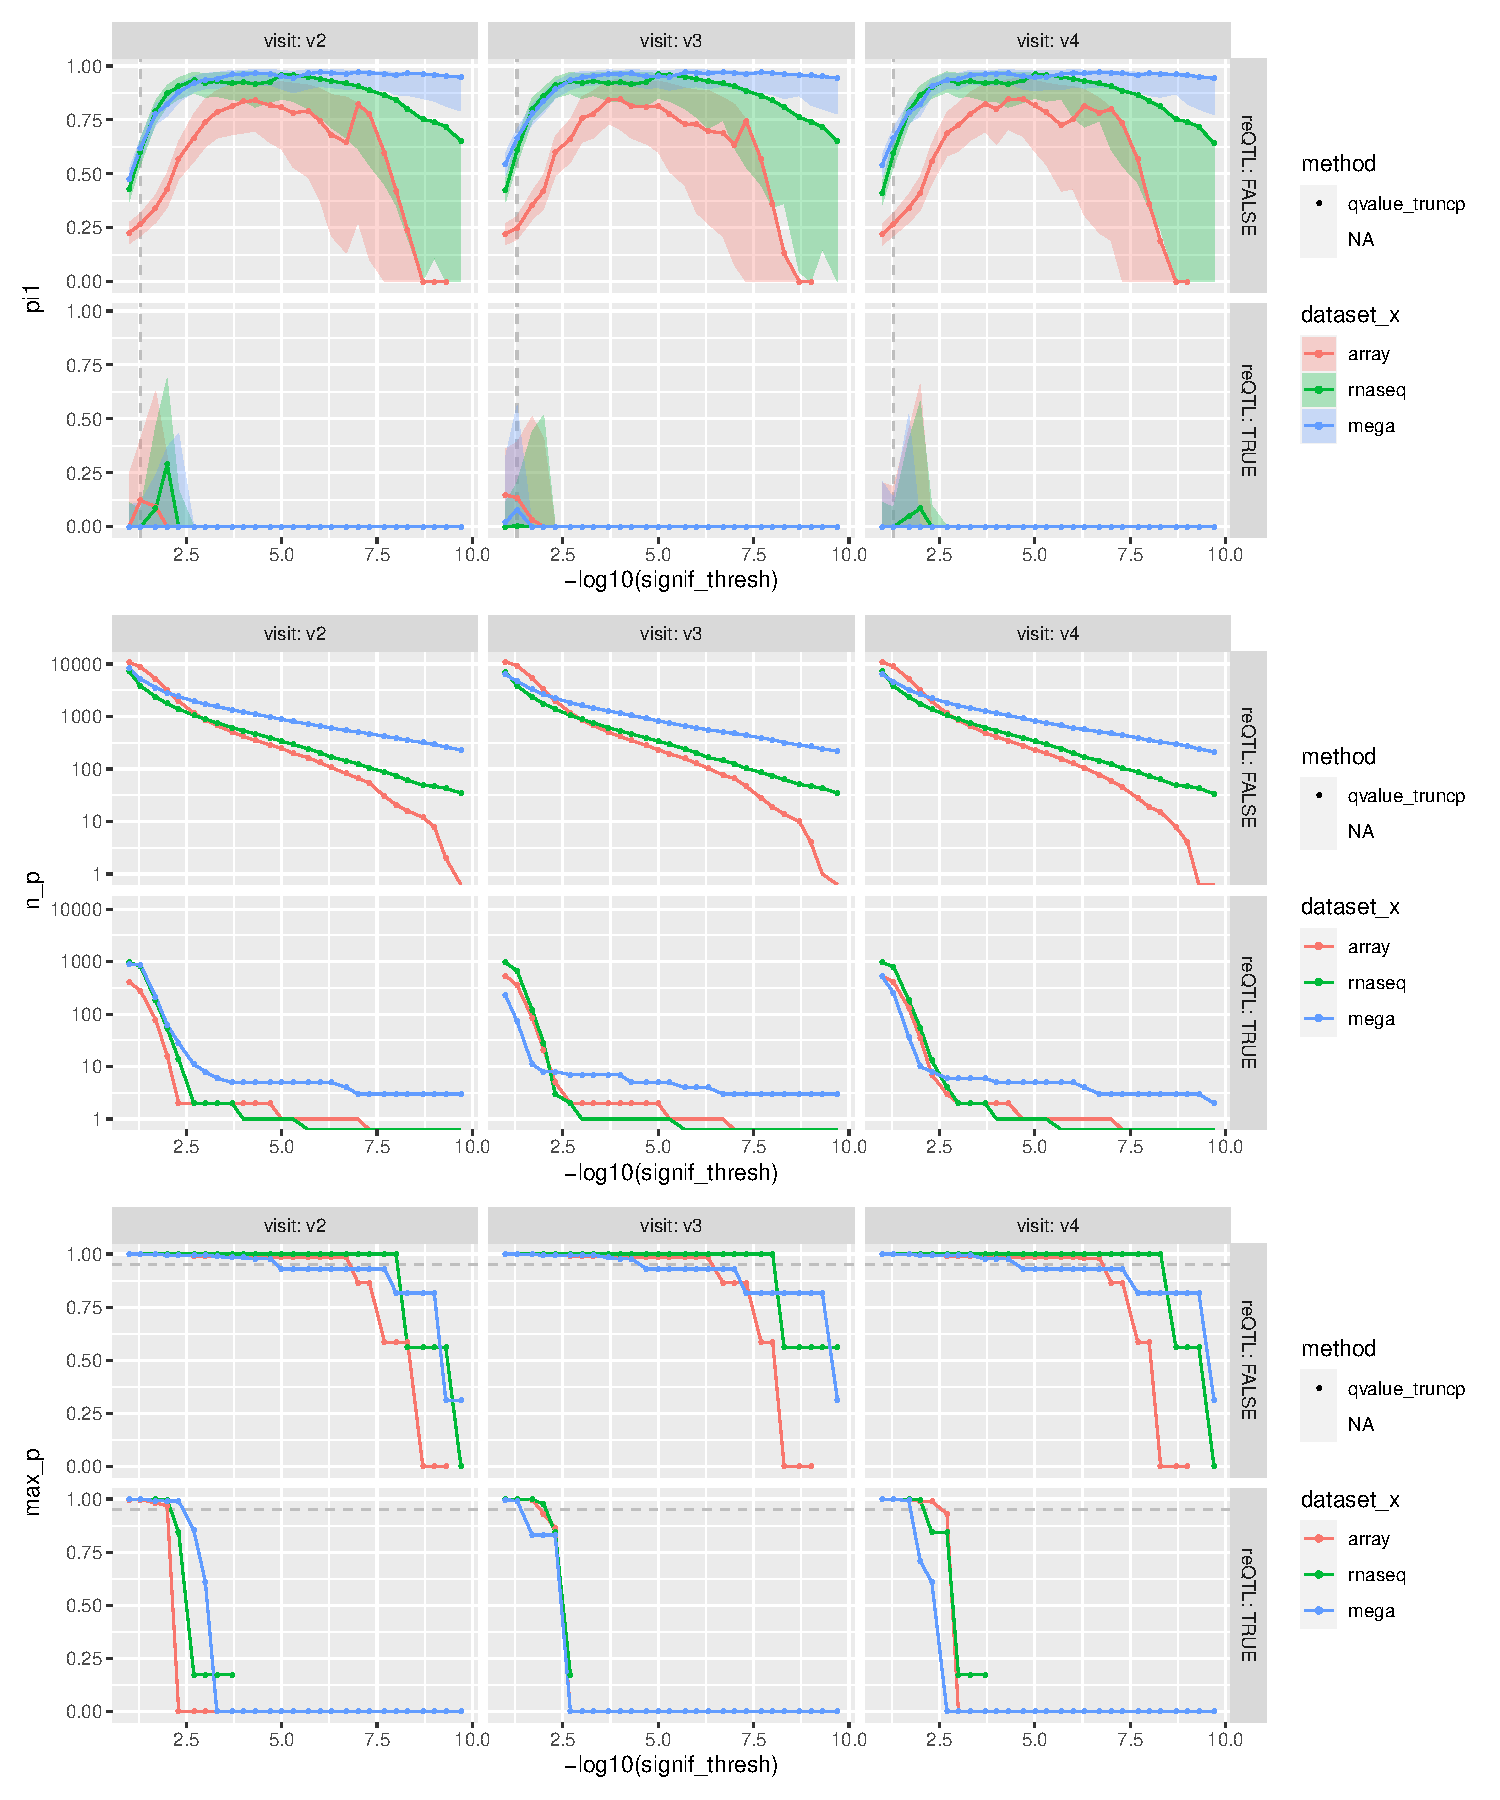
\includegraphics[width=1.0\textwidth,page=1]{mainmatter/figures/chapter_03/compute_pi1.pi1_by_thresholds.pdf}
    \caption{
        \textbf{
            Replication rate $\pi_1$ of \gls{HIRD} \gls{eQTL} in GTEx whole blood \gls{eQTL} reference data.
        }
        Three \gls{eQTL} analyses were run in \gls{HIRD}: array-only, \gls{RNAseq}-only, and a mega-analysis of the two.
        Panels are stratified into shared \glspl{eQTL} and \glspl{reQTL}.
        The top panel shows $\pi_1$ replication in each analysis version as a function of the significance threshold (lfsr), with the shaded region for showing the 5th-95th percentile range of 1000 bootstraps.
        Vertical line shows $lfsr = 0.05$.
        The middle panel shows the number of significant \gls{HIRD} \gls{eQTL} present in GTEx; this is the number of \pvalues{} available for computing $\pi_1$.
        The computation is more reliable when there are \textapprox{1000} or more.
        The bottom panel shows the maximum nominal GTEx \pvalue{} for those variants use to compute $pi_1$.
        The computation is more reliable when the maximum is near 1.
        Effect of \gls{HIRD} lfsr threshold on GTEx whole blood replication rate ($\pi_1$), number of \pvalues{} used to compute $\pi_1$, and maximum \pvalue{} among those \pvalues{}; 
    }
    \label{fig:hird_eQTL_pi1vsGTExWholeBlood}
\end{figure}

\subsection{Genotype interactions with cell type abundance}
\label{subsec:hird_reQTL_methods_cellTypeInteraction}

% TODO Figure out what DAG model is appropriate, maybe see
% https://doi.org/10.1111/bmsp.12217
%
% NOTE: Effect modification can be present with no interaction; interaction can be present with no effect modification. \autocite{vanderweele2009DistinctionInteractionEffect}
If the abundance of a particular cell type does truly modify the \gls{eQTL} effect, 
then an interaction term between genotype and cell type abundance is required.
As the additivity assumption no longer holds, a \textit{ceteris paribus} interpretation does not make sense,
as the effect of genotype holding cell type abundance constant depends on what value of cell type abundance you choose.
I
% TODO: OVB by setting interaction coefficient to zero
% http://consirt.osu.edu/wp-content/uploads/2014/10/CONSIRT-Working-Papers-Series-9-Mikucka_Sarracino_Dubrow.pdf
% Most importantly, the figures document thatwrongly  omitting  an  interaction  term  (Figure  3)  can  bias  the  estimates  much  more  thanwrongly including an interaction term (Figure 4).
One cannot adjust for modification just by including the main effect for cell type abundance,
Wrongly omitting a significant interaction term between cell abundance and genotype biases the estimation of the two main effects\footnote{When a variable that is the function of another explanatory variable is omitted, this is known as functional form misspecification in the field of econometrics, a special case of omitted variable bias. Also see \textcite{mikucka2015CostsBenefitsIncluding} for a review of bias caused by omitting significant interaction terms.}.
% Also see:
% https://stats.stackexchange.com/questions/263324/how-can-the-regression-error-term-ever-be-correlated-with-the-explanatory-variab
% the realisation of the error term, the residuals, is forced to be uncorrelated, hence you get a biased estimate
Given the modest sample size, I used a two-stage approach,
where tests for interaction are only performed at a subset of tests.
% Unfortunately, there seems to be no consensus between these studies for controlling the interaction effect tests for multiple testing.
%
% Strange custom 5% FDR: westra2015CellSpecificEQTL
% Bonferroni: kim-hellmuth2017GeneticRegulatoryEffects
% Benjamini-Hochberg FDR: kim-hellmuth2017GeneticRegulatoryEffects
% Benjamini-Hochberg procedure, and a 0.15 FDR threshold: peters2016InsightGenotypePhenotypeAssociations
%
% https://www.jmp.com/support/help/en/15.2/index.shtml#page/jmp/effect-heredity.shtml
% The principle of effect heredity relates to the inclusion in the model of lower-order components of higher-order effects. The motivation for this principle is observational evidence that factors with small main effects tend not to have significant interaction effects.
% NOTE: this is not strictly effect heredity, as I do not consider the significance of cell proportion terms
%
The key to the two-stage approach is if
the main effect estimates from main effect-only models (stage one) are used to filter \glspl{SNP} for second stage testing,
and are also independent from the interaction effect estimates in stage two,
then the type I error can be controlled based on the number of interactions that are actually tested, rather the number of interactions that could have been tested for \autocite{kooperberg2008IncreasingPowerIdentifying,peters2016InsightGenotypePhenotypeAssociations}.
It is unclear whether this assumption holds in practice, as being able to detect a main effect at least implies that gene is sufficiently expressed for \gls{eQTL} mapping.
Nevertheless, the two-stage approach is often used for \gls{eQTL} mapping with an interaction term \autocite{westra2015CellSpecificEQTL,peters2016InsightGenotypePhenotypeAssociations,kim-hellmuth2017GeneticRegulatoryEffects,davenport2018DiscoveringVivoCytokineeQTL}.
As the main purpose of my interaction analyses is scanning for cell type effects at detected \glspl{reQTL},
I chose to test for interactions only at the lead \gls{eQTL} variant for each gene with a significant main \gls{eQTL},
then apply the \gls{BH} \gls{FDR}, as used by others\autocite{peters2016InsightGenotypePhenotypeAssociations,kim-hellmuth2017GeneticRegulatoryEffects}.

Models with interactions between genotype and other predictors were fit using \software{lme4qtl} \autocite{ziyatdinov2018Lme4qtlLinearMixed}.
The model specification was identical to \cref{eq:hird_reQTL_limix_model} except the addition of three interaction terms between genotype and each xCell score.
Significance was assessed using the \gls{LRT} versus the nested model with no interaction terms.
Note that although PEER factors are correlated with xCell scores (\cref{fig:}), 
\textcite{kim-hellmuth2020CellTypeSpecific} also used this approach, claiming that interaction term between genotype and xCell scores should still be interpretable.
I attribute their claim to the fact that there are no interaction terms between genotype and PEER factors, so the coefficients for each genotype-xCell scores interactions still have their standard interpretation: $\beta_x + \beta_{cx}c$ increase in log2 expression per unit of effect allele dosage, where $\beta_x$ is the main effect of genotype, $\beta_{cx}$ is the interaction effect, and $c$ is xCell score.

\subsection{Gene set enrichment analyses}
\label{subsec:hird_reQTL_geneSetEnrichment}

Ranked gene set enrichment analyses with \software{tmod::tmodCERNOtest} were conducted as described in \cref{subsec:hird_dge_geneSetEnrichment},
using \glspl{BTM} from \textcite{li2013MolecularSignaturesAntibody} (prefixed \enquote{LI}).

Gene set overrepresentation analyses were run with 
\software{tmod::tmodHGtest} which implements the hypergeometric test for enrichment in \glspl{BTM}, with \gls{BH} \gls{FDR} control at 0.05.
Gene set overrepresentation analyses were also run with 
\software{gprofiler2::gost} \autocite{raudvere2019ProfilerWebServer},
which derives gene sets from
    Gene Ontology,
    pathway databases (KEGG, Reactome, WikiPathways),
    regulatory motif databases (TRANSFAC, miRTarBase),
    pathway databases (KEGG, Reactome, WikiPathways),
    protein databases (Human Protein Atlas, CORUM),
    and phenotype ontologies (HP).
The default \software{gprofiler2} g:SCS method was used to control for multiple testing while accounting for the hierarchical structure of certain gene set databases like the Gene Ontology.
In both tests, 
the 13570 genes assayed by both array and \gls{RNAseq} were used as a custom background set.
% (\texttt{domain\_scope='custom'}) for gprofiler

\subsection{Statistical colocalisation}
\label{subsec:hird_reQTL_coloc}

Published \gls{GWAS} and \gls{QTL} summary statistics were downloaded for statistical colocalisation with per-timepoint \gls{HIRD} \gls{eQTL} summary statistics.
Clinical blood count \gls{QTL} maps generated by \textcite{astle2016AllelicLandscapeHuman} in \num{173480} European-ancestry participants were downloaded from \url{ftp://ftp.sanger.ac.uk/pub/project/humgen/summary_statistics/human/2017-12-12/hematological_traits/}.
\gls{eQTL} maps in 15 \gls{FACS}-sorted immune cell types generated by \textcite{schmiedel2018ImpactGeneticPolymorphisms} in a multi-ethnic cohort of 91 donors,
were downloaded from the eQTL Catalogue (\autocite{kerimov2020EQTLCatalogueCompendium}, release 1 - January 2020, \url{https://www.ebi.ac.uk/eqtl/}).
These included
three naive innate immune cell types: 
    classical monocytes (CD14\textsuperscript{high}CD16\textsuperscript{-}),
    non-classical monocytes (CD14\textsuperscript{-}CD16\textsuperscript{+}),
    and \gls{NK} cells;
four naive adaptive immune cell types:
    B cells, CD4+ T cells, CD8+ T cells, and regulatory T cells (Treg);
CD4+ T cells and CD8+ T cells stimulated with anti-CD3 anti-CD28 for 4 hours;
and six CD4+ memory T cell subsets:
    Th1, Th1/Th17, Th17, Th2, and memory Tregs.
\Gls{IBD} \gls{GWAS} summary statistics generated by \textcite{delange2017GenomewideAssociationStudy} in a total of \num{59957} European ancestry samples were downloaded from \url{https://www.ebi.ac.uk/gwas/studies/GCST004131}.
Datasets were converted to GRCh38 coordinates with \software{rtracklayer::liftOver},
and harmonised to a standard format, matching variants between studies by genomic position and effect allele.

Multi-trait Bayesian colocalisation was performed using \software{HyPrColoc} \autocite{foley2019FastEfficientColocalization}.
\software{HyPrColoc} uses the pattern of per-variant summary statistics (betas and standard errors) from multiple traits in a locus to partition traits into clusters, where each cluster contains traits that share a causal variant.
This can be seen as a multi-trait extension of pairwise Bayesian colocalisation methods such as \software{coloc} \autocite{giambartolomei2014BayesianTestColocalisation}.
Multi-trait colocalisation is more powerful than pairwise colocalisations for detecting causal variants shared between more than two traits,
and large numbers of traits can be analysed simultaneously in a computationally efficient manner.
The method formally assumes that studies generating the summary statistics for each trait are independent,
but performs well even when there is complete sample overlap between traits \autocite{foley2019FastEfficientColocalization}.
% https://github.com/jrs95/hyprcoloc/issues/1
% As the model assumes there is at most one causal variant per phenotype, the way the model is set up there is no need to consider LD between variants. This follows from the Giambartolomei coloc method (PMID: 24830394), on which HyPrColoc is based.
% The LD matrix is only required in HyPrColoc to modify the variant priors when the traits are from non-overlapping samples in conjunction with a phenotype correlation matrix (there is a complex argument as to why this is necessary, which @cnfoley can give you). Although, in simulations treating phenotypes as if they were from independent samples, even if they were not, often out-performed trying to account for the possible correlation between phenotypes caused by analysing the phenotypes in the same participants. So, our general advice is to just run the standard model, and to not worry about global phenotype correlation caused through analysis of overlapping samples.
If studies are non-independent, 
it is assumed the \gls{LD} structure is the same across those studies (which holds in the case of multiple \gls{QTL} maps generated from the same individuals).
Each trait is assumed to have no more than one causal variant in the locus.
Finally, it is assumed the causal variants for each trait are present in the input.

As with any Bayesian colocalisation method, the choice of priors and other algorithm parameters is influential.
\software{HyPrColoc} implements variant-level priors where the prior depends on the number of traits a variant is causally associated with.
\texttt{prior.1} is the prior probability that a variant is causal for one trait (default = \num{1e-4}) and
1 - \texttt{prior.2} specifies the prior probability that a variant is causal for an additional trait, given it is causal for one trait (default = \num{0.98}).
The prior for a variant being causal for a third trait given it is causal for two traits is $1-(\texttt{prior.2})^2$, and so on.
In the two trait case, the setup is identical to \texttt{coloc} \autocite{giambartolomei2014BayesianTestColocalisation}.
\texttt{prior.2} tends to be more influential than \texttt{prior.1}, as it controls the probability of association with more and more traits.

The posterior probability of colocalisation for a cluster of traits is the product of regional association and alignment probabilities.
% Calculated from variant level probabilities?
The regional association probability is the probability there is a shared association region within the locus for all the traits in the cluster, containing one or more causal variants.
The alignment probability is the probability that regional association is due to a single causal variant, rather than one or more variants in strong \gls{LD}. 
A branch and bound algorithm is run, starting with all traits in one cluster,
then recursively partitioning traits into subsets, assessing regional association and alignment probabilities for subsets at each iteration.
The end result is clusters of traits sharing a causal variant, with each cluster having a distinct causal variant.
% Traits left in their own cluster do not colocalise with any other traits.
Only clusters with more than one trait and regional association and alignment probabilities above \texttt{reg.thresh} (default=0.5) and \texttt{align.thresh} (default=0.5) are reported.

% NOTE: https://rdrr.io/github/jrs95/hyprcoloc/f/vignettes/hyprcoloc.Rmd
In sensitivity analyses using the \software{sensitivity.plot} function,
% As the number of traits in the sample increases the default choice of $prior.1$ may be become increasingly inappropriate.
% However, to guide analyses we suggest comparing results using the default $10^{-4}$ with those when $prior.1 = 10^{-5}$, i.e. an order of magnitude reduction in "prior.2", for sensitivity analyses.
% NOTE: if doing this genome-wide, try fgwas (cano 2020), enloc (kim-hell 2020)?
I fixed the less influential \texttt{prior.1} at the default of \num{1e-4}, 
then iterated over combinations of
% When using the variant specific prior, results tend to be most sensitive to the choice of $prior.2$ as this controls the prior probability of each additional colocalized trait.
four choices of \texttt{prior.2} (0.98, 0.99, 0.995, 0.999),
% Note, these parameter choices are a consequence of extensive testing in simulation scenarios, aiming to maximise the true detection rate whilst minimising the number of false positives. We therefore DO NOT recommend reducing the value of either of these parameters. The defaults should be viewed as lower bounds.
% We therefore DO NOT recommend reducing the value of either of these parameters. The defaults should be viewed as lower bounds.
five choices of \texttt{reg.thresh} (0.5, 0.6, 0.7, 0.8, 0.9),
and five choices of \texttt{align.thresh} (0.5, 0.6, 0.7, 0.8, 0.9).
Each range starts at the default value and becomes more stringent, 
requiring stronger and stronger evidence for clusters of colocalised traits to be identified.

\section{Results}

\subsection{Mapping reQTLs in the HIRD cohort}

To characterise the effect of common host genetic variation on expression response to Pandemrix,
I mapped cis-\glspl{eQTL} for each gene (\SI{\pm1}{\mega\bp} of the \gls{TSS}) within each timepoint condition (baseline, day 1, and day 7),
then conducted joint analysis of all three timepoints with \software{mashr} \autocite{urbut2018FlexibleStatisticalMethods} to obtain per-timepoint posterior effect sizes, posterior standard errors, and measures of significance (\gls{lfsr}).
% NOTE: 13570 includes X chr, but technically we should exclude those:
% Requires sex-specific methods due to copy number differences between males and females, and X-inactivation of a random allele in females \autocite{soranzo2009GenomewideMetaanalysisIdentifies}.
At \gls{lfsr} < 0.05, \num{6887/13570} genes (\percentage{0.5075166}) were eGenes (genes with a significant \gls{eQTL}) in at least one timepoint.
The most significant tested variant over all timepoints was selected as the lead variant for each gene,
then \glspl{reQTL} were defined by comparing the effect size of this lead variant between each pair of timepoints.
This guards against differences in effect size from differential tagging efficiency (of an assumed single causal variant), 
which might occur if different variants were compared across timepoints.
\cref{fig:hird_eQTL_upset_mega} shows patterns of sharing over timepoints for the lead variant for each of the \num{13570} genes,
illustrating the difference between calling \gls{reQTL} using a significance threshold versus the difference in betas approach.
For example, there were 85 \gls{eQTL}-eGene pairs significant only at day 1 post-vaccination ($lfsr < 0.05$); of these only \num{40/85} are \glspl{reQTL} by the difference in betas method.
The difference in betas method is more strict because calling by significance alone would call a \gls{reQTL} for an \gls{eQTL} with lfsr = 0.049 at baseline and lfsr = 0.051 at day 1, even if the effect sizes are similar.
Shared \glspl{eQTL} were well-replicated in GTEx whole blood (\cref{fig:hird_eQTL_pi1vsGTExWholeBlood}).

The largest number of eGenes was detected at baseline, reflecting the larger sample size compared to other timepoints.
Most \glspl{eQTL} were shared across timepoints; 
these were also the strongest \glspl{eQTL} in terms of both maximum absolute beta and \gls{PVE} across timepoints, highlighting the power advantage for mapping shared effects granted by joint analysis.
\num{1154/6887} (\percentage{0.1675621}) \glspl{eQTL} were classified as \glspl{reQTL} based on difference in effect size (beta) between any pair of timepoints (nominal p < 0.05).
Of these, 
\num{690/1154} were \glspl{reQTL} between both day 1 vs. baseline and day 7 vs. baseline, 
and only \num{23/1154} were unique to the day 7 vs. day 1 comparison, 
indicating most \gls{reQTL} effects were differences between pre- and post- vaccination (\cref{fig:hird_reQTL_pairwise_venn}).

\begin{figure}
    \centering
    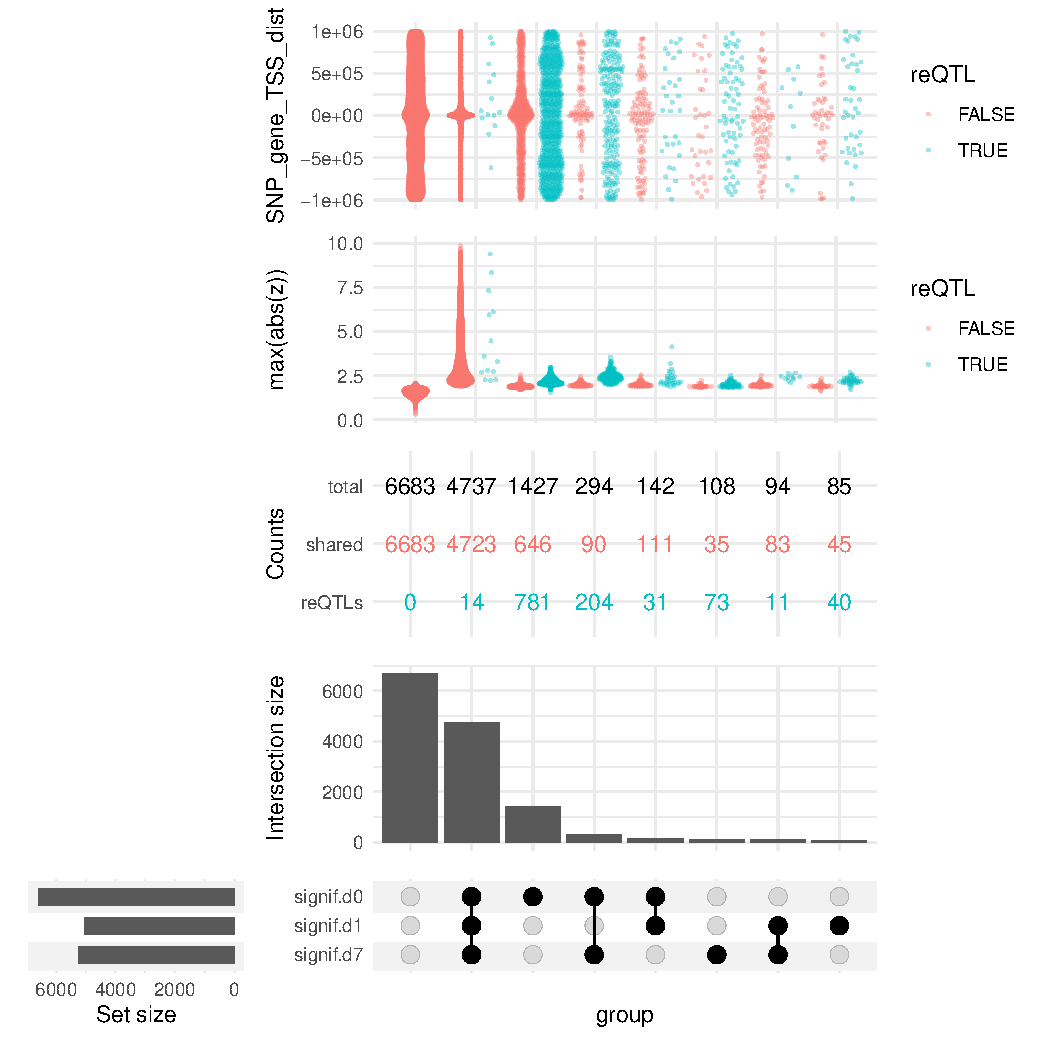
\includegraphics[width=1.0\textwidth]{mainmatter/figures/chapter_03/compare_dge_eqtl.upset.pdf}
    \caption{
        \textbf{Summary of HIRD eQTL mapping at 13570 genes in a mega-analysis of array and RNAseq, binned by patterns lead variant significance over the three timepoints.}
        The most significant variant for each gene over all timepoints was chosen as the lead variant.
        Significant eQTLs (lfsr < 0.05) were found at \num{6887/13570} eGenes.
        These were classified as reQTLs if there was a significant difference in beta (nominal p < 0.05) between any pair of timepoints,
        given that the eQTL was significant in at least one of those two timepoints.
        Counts of shared and reQTLs; and distribution of maximum beta and \gls{PVE} across timepoints, for variants in each bin are shown.
    }
    \label{fig:hird_eQTL_upset_mega}
\end{figure}

\begin{figure}
    \centering
    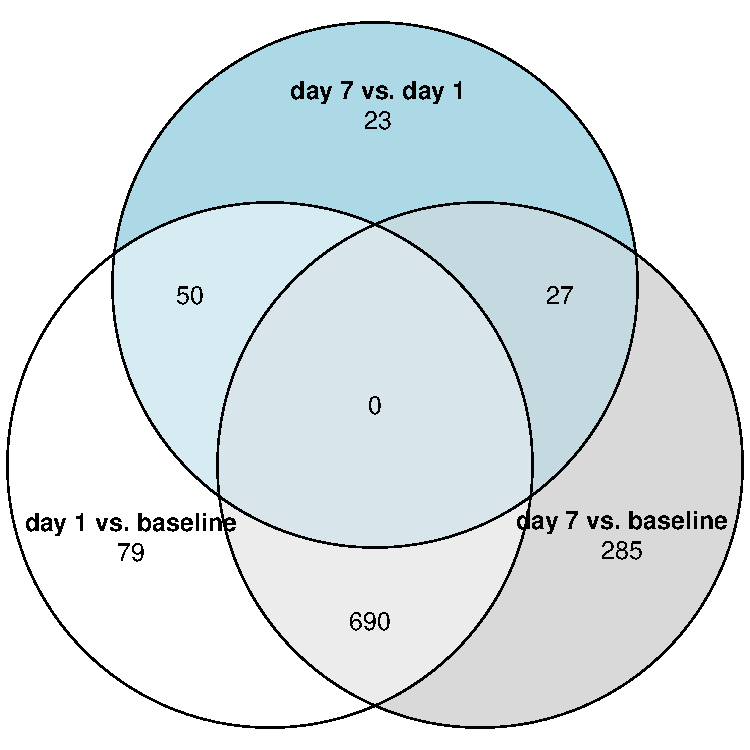
\includegraphics[width=0.6\textwidth]{mainmatter/figures/chapter_03/compare_dge_eqtl.pairwise_reQTL_venn.pdf}
    \caption{
        \textbf{\glspl{reQTL} were observed for 1154 unique eGenes, where the lead \glspl{eQTL} had a significant difference in beta between pairs of timepoints (nominal p < 0.05).}
    }
    \label{fig:hird_reQTL_pairwise_venn}
\end{figure}

\subsection{Characterising reQTLs post-vaccination}

To characterise the eGenes associated with post-vaccination \glspl{reQTL},
I ranked eGenes by the increase in \gls{PVE} for their associated \glspl{reQTL} from baseline to day 1 and baseline to day 7,
then performed ranked gene set enrichments with \software{tmod::tmodCERNOtest}.
%
% Possible Ranking metrics for ranked enrichments
%     PVE: prefers large maf and high betas since it squares the beta. even if the beta does not change so much. ignores sign.
%     beta:
%     p: ignores sign
%     Z score:
%
The same four modules were significant at both post-vaccination timepoints:
\enquote{immune activation - generic cluster} (LI.M37.0, day 1 $\text{\gls{FDR}} = \num{1.283444e-06}$, day 7 $\text{\gls{FDR}} = \num{3.391644e-06}$),
\enquote{enriched in monocytes (II)} (LI.M11.0, day 1 $\text{\gls{FDR}} = \num{4.688999e-03}$, day 7 $\text{\gls{FDR}} = \num{1.881201e-02}$),
\enquote{cytoskeleton/actin (SRF transcription targets)} (LI.M145.0, day 1 $\text{\gls{FDR}} = \num{2.071726e-02}$, day 7 $\text{\gls{FDR}} = \num{2.036488e-02}$),
and \enquote{MHC-TLR7-TLR8 cluster} (LI.M146, day 1 $\text{\gls{FDR}} = \num{2.071726e-02}$, day 7 $\text{\gls{FDR}} = \num{2.036488e-02}$).
The enrichments are weak but consistent with immune activation driving post-vaccination \glspl{reQTL}.
Given that TLR7 and TLR8 are primarily expressed in monocytes, macrophages and \glspl{DC} \autocite{cervantes2012TLR8ForgottenRelative},
and \gene{SRF} is a regulator of the cytoskeleton in macrophages \autocite{sullivan2011SerumResponseFactor}, 
there is suggestive evidence \glspl{reQTL} may be enriched in genes specific to these phagocytotic \glspl{APC}.

Changes in \gls{PVE} do not capture changes in allelic direction.
I classified post-vaccination \glspl{reQTL} into one of three effect types:
magnified, where the beta increases after vaccination but remains the same sign;
dampened, where the beta decreases after vaccination but remains the same sign;
and opposite, where the allelic direction changes after vaccination.
As \gls{lfsr} quantifies uncertainty in the sign of the effect, I do not make this classification for \glspl{reQTL} that are not significant both at baseline and post-vaccination---the effect type for these are unclear.
The classifications are shown in \cref{fig:hird_eQTL_zSharing_vs_TSSdist_mega}, plotting all 6887 shared or \gls{reQTL} by their distance relative to the eGene \gls{TSS}.
% TODO: is the gap still there if you use beta not pm?
Shared \glspl{eQTL} have \textit{z}-statistics for difference in betas close to z, and are concentrated close to the \gls{TSS} as expected, 
\gls{reQTL} had a distribution of mostly negative \textit{z}-statistics clearly separated from the shared \glspl{eQTL} at both day 1 and 7,
and these were mostly unclear or opposite rather than dampened effect types.
Many of these unclear effects may actually be dampening, 
but as the sample size is greatest at baseline, 
dampening effects are hard to distinguish from drops in power at post-vaccination timepoints, 
whereas an opposite effect significant in both timepoints is unambiguous.
% NOTE: opposite effects were nominally significant even without mashr

\begin{figure}
    \centering
    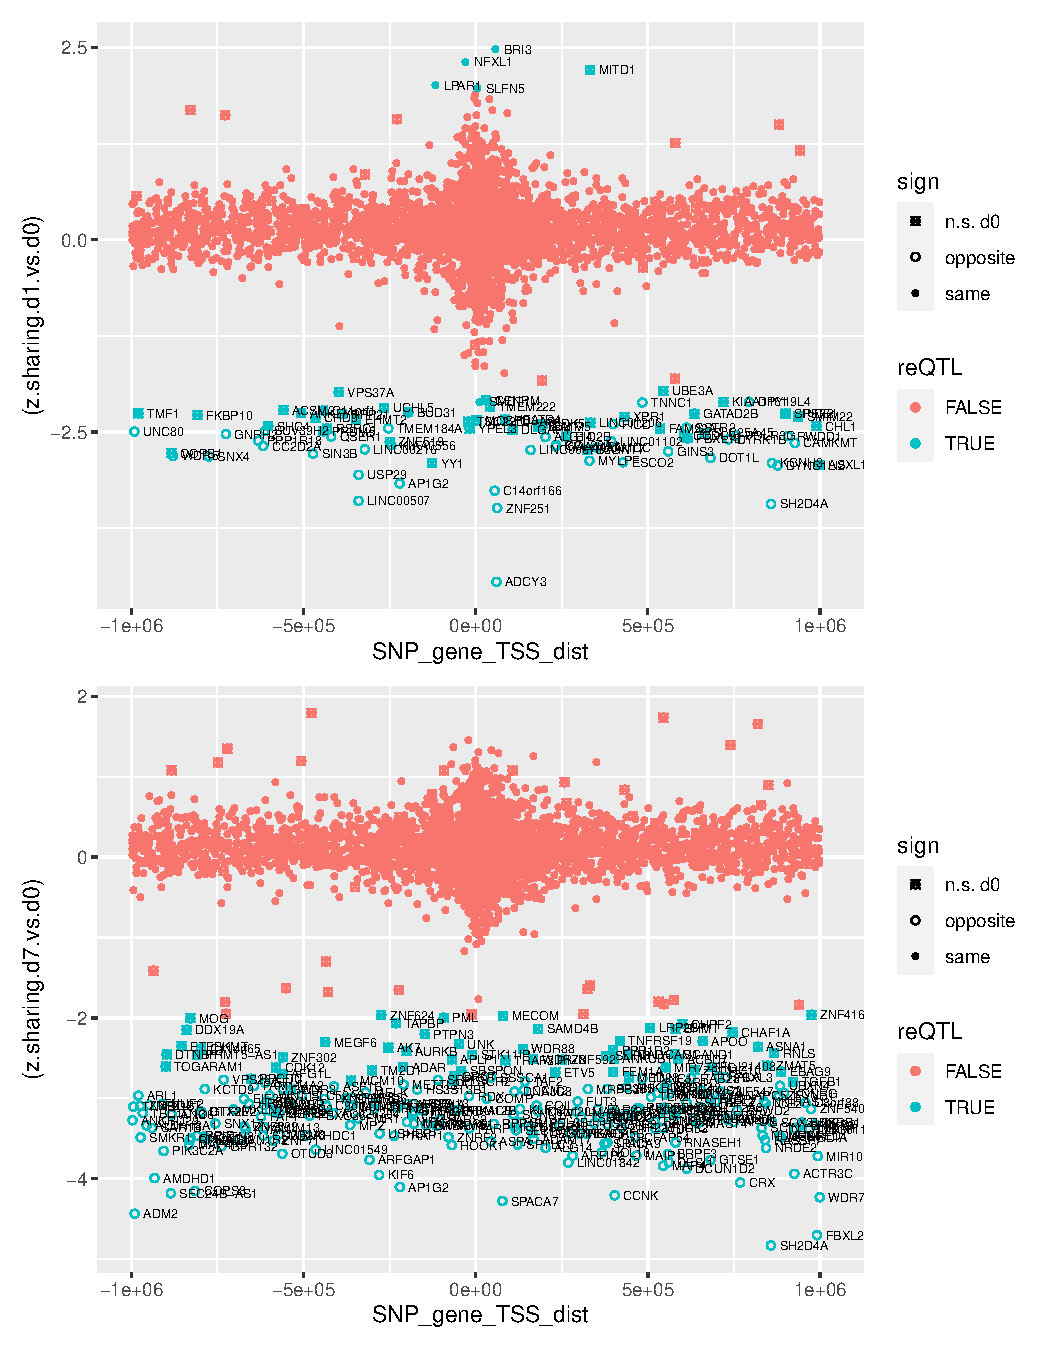
\includegraphics[width=1.0\textwidth]{mainmatter/figures/chapter_03/compare_dge_eqtl.z_sharing.vs.SNP_gene_TSS_dist.pdf}
    \caption{
        \textbf{\textit{z}-statistic for difference in beta post-vaccination versus baseline for shared and \glspl{reQTL}, stratified by distance from the eGene \gls{TSS}.}
        For each plot, all \glspl{eQTL} significant in either timepoint are shown.
        Shared \glspl{eQTL} can only have shared effect type.
        an unclear effect type indicates the \gls{eQTL} in question was not significant in both timepoints.
        Allelic direction of effect is aligned so that the beta at baseline is positive. 
    }
    \label{fig:hird_eQTL_zSharing_vs_TSSdist_mega}
\end{figure}

\glspl{reQTL} also tended to be distributed evenly across the entire \textit{cis}- window,
raising the question or whether they are enriched in false positives.
A nominal p < 0.05 threshold, although stricter than many types of threshold (see \cref{subsec:hird_reQTL_methods_definingSharedAndreQTLs}), may still be too lax for calling \glspl{reQTL},
so I applied a stronger \gls{BH} \gls{FDR} threshold of 0.2.
At this threshold, the only remaining \gls{reQTL} was at day 1 was for \gene{ADCY3} (nominal p = \num{8.676917e-06}, FDR = \num{0.1177458})---the next smallest FDR value was 0.6490604.
At day 7, 676 significant \gls{reQTL} had \gls{FDR} < 0.2, of which 221 were opposite effects.
Gene set over-representation analysis on the set of 221 eGenes to identify a shared biological signature 
was relatively uninformative, and revealed only one enrichment for genes \gene{PRKACB}, \gene{PRKACA}, \gene{SAR1B} and \gene{APOE} in \enquote{Plasma lipoprotein assembly} (Reactome pathway identifer R-HSA-8963898, set size = 11, adj. p = \num{0.00691834}).
Since \textcite{fairfax2012GeneticsGeneExpression} found cases of opposite \gls{reQTL} effects between B cells and monocytes, and B plasma cells increase in abundance at day 7 but not monocytes \autocite{sobolev2016AdjuvantedInfluenzaH1N1Vaccination},
I also performed gene set over-representation analysis on the same set of gene with \glspl{BTM} to detect if gene related to B cells were enriched.
No significant enrichments were identified.

\subsection{Exploring possible mechanisms generating reQTLs}

\subsubsection{Differential gene expression of reQTL eGenes}

As gene set analyses based on the effect sizes of \glspl{reQTL} at different timepoints had been largely uninformative,
I considered whether \gls{reQTL} could be characterised by shared mechanisms.
One mechanism that could generate \glspl{reQTL} effects is differential expression, where an \gls{eQTL} is not detected at baseline because the eGene is not expressed, and vaccine-stimulated upregulation reveals the effect post-vaccination.
\cref{fig:hird_eQTL_zSharing_vs_TSSdist_mega} also shows whether each eGene was up or downregulated at the timepoint based on the \gls{DGE} analyses in \cref{ch:hird_DGE}.
Visually, a large number of \gls{reQTL} occur without corresponding differential expression.
Statistically, compared to genes without reQTL,
genes with \glspl{reQTL} were less likely be differentially expressed post-vaccination at day 1 (\percentage{0.2649573} for genes with reQTL, \percentage{0.4227119} for genes without reQTL, Fisher's test p < \num{2.2e-16}).
This was also the case when restricting the scope to only eGenes (\percentage{0.2649573} for genes with reQTL, \percentage{0.4791946} for genes with shared eQTL, Fisher's test p < \num{2.2e-16}).

At day 7, 
no significant difference was observed comparing to genes without a reQTL (\percentage{0.02195609} for genes with reQTL, \percentage{0.01368555} for genes without reQTL, Fisher's test p = \num{0.05088}),
but compared to genes with shared \gls{eQTL},
genes with \gls{reQTL} were more likely to be upregulated
(\percentage{0.02195609} for genes with reQTL, \percentage{0.01068966} for genes with shared eQTLs, Fisher's test p = \num{0.005015}).
Twenty-two genes with both day 7 \gls{reQTL} and upregulated expression were strongly enriched within gene sets related to the cell cycle, such as
\enquote{mitotic cell cycle} (Gene Ontology biological process term GO:0000278, term size = 914, intersection size = 12, \software{gprofiler2::gost} adj. p = \num{0.0001419083}),
\enquote{cell cycle (I)} (LI.M4.1, module size = 137, intersection size = 12, \software{tmodHGtest} $\text{\gls{FDR}} = \num{1.409575e-16}$),
and \enquote{mitotic cell cycle in stimulated CD4 T cells} (LI.M4.5, module size = 33, intersection size = 3, \software{tmodHGtest} $\text{\gls{FDR}} = \num{1.409575e-16}$).
% Small and oppopste between cell types, can we find enrichment?
However, these 22 genes previously appeared in \cref{fig:hird_eQTL_zSharing_vs_TSSdist_mega} as having \gls{reQTL} with decreased or opposite effect at day 7 versus baseline,
making it implausible that the generating mechanism is increased detection power due to upregulation.
The enrichment for cell cycle is likely driven by the \gls{DGE} signal alone,
especially as similar cell cycle gene modules were detected to be strongly upregulated at day 7 in \cref{subsec:hird_dge_adaptive_immune_day7}.

The presence of \gls{reQTL} without \gls{DGE} is exemplified at the strongest
\gls{reQTL} at each day.
The only significant \gls{reQTL} on day 1 at FDR < 0.2 was for \gene{ADCY3} (\cref{fig:hird_eQTL_ploteQTL_ADCY3}).
At day 1, the \gls{PVE} for this \gls{reQTL} associated with \gene{ADCY3} explained \percentage{0.01862996} of expression variation at day 0, increasing to \percentage{0.14075782} at day 1,
yet the gene was not differentially expressed from baseline to day 1 (log2FC=\num{0.10373360}, lfsr=\num{0.2569459}).
% Overall, only 5/68 (\percentage{0.1323529}) genes with \glspl{reQTL} that explain more variation at day 1 were upregulated at day 1 vs. day 0; 5/226 (\percentage{0.02212389}) for day 7 vs. day 0.
%
% The strongest reQTL at day 7 is one such opposite sign effect;
% \gene{SH2D4A} has constitutive expression in T cells, B cells, macrophages, and \glspl{DC},
% encoding a adapter protein involved in intracellular signal transduction\footnote{\url{https://doi.org/10.1111/j.1600-065X.2009.00829.x}}.
At day 7 the strongest \gls{reQTL} was at \gene{SH2D4A} (nominal p difference in betas = \num{1.369564e-06}, BH FDR = \num{0.01747935}, \cref{fig:hird_eQTL_ploteQTL_SH2D4A}).
Here, the \gls{reQTL} variant explained similar amounts of expression variation at day 0 (\gls{PVE}=\percentage{0.08229266}) and day 7 (\gls{PVE}=\percentage{0.08956865}), with opposite directions of effect (\cref{fig:hird_eQTL_ploteQTL_SH2D4A}).
Again, there was no differential expression.
There is strong evidence that many post-vaccination \glspl{reQTL} are generated by mechanisms unrelated to \gls{DGE}.

\begin{figure}
    \centering
    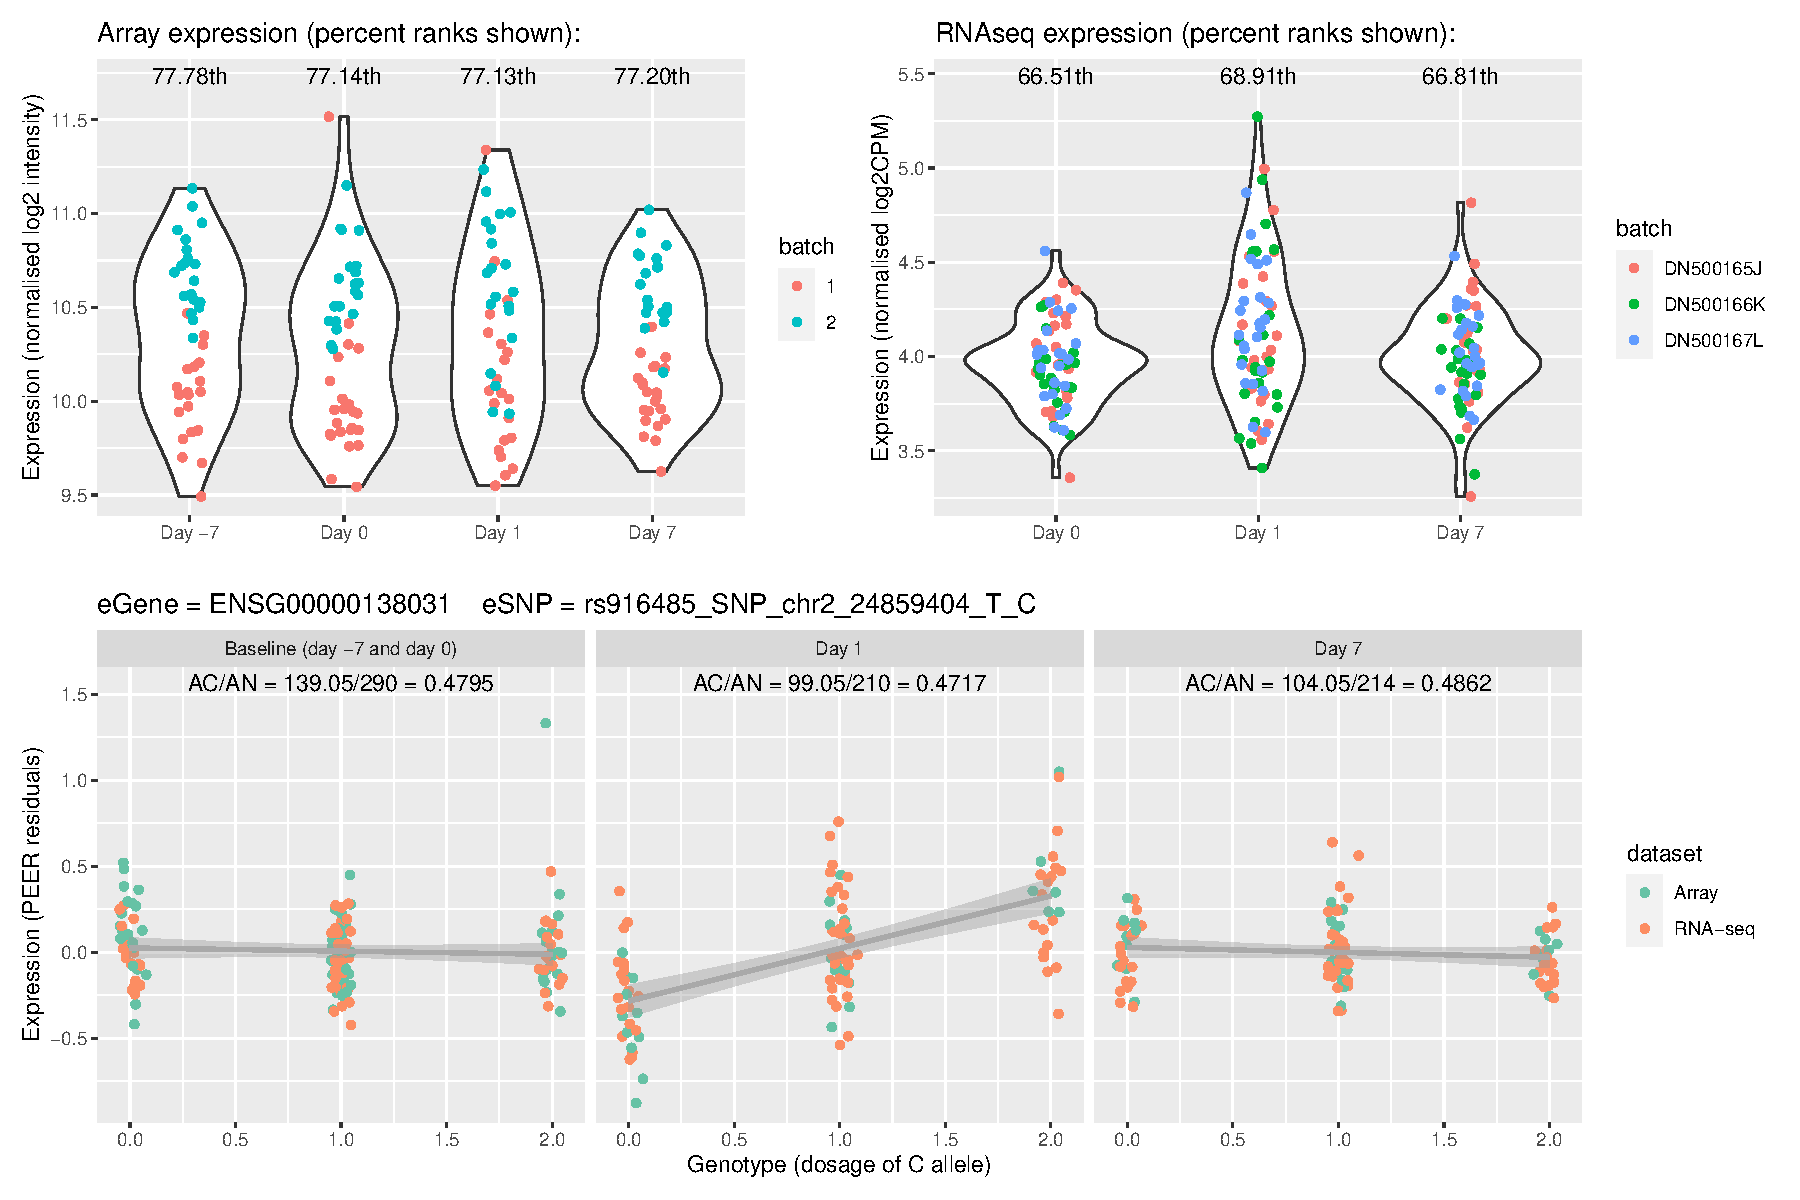
\includegraphics[width=1.0\textwidth,page=1]{mainmatter/figures/chapter_03/plot_dge_eqtl_genotypes.ENSG00000138031,rs916485_SNP_chr2_24859404_T_C.pdf}
    \caption{
        \textbf{Expression and lead \gls{eQTL} of \gene{ADCY3} over study timepoints.}
        Normalised array (top-left) and \gls{RNAseq} (top-right) expression before batch effect correction with ComBat and \gls{eQTL} mapping. 
        Bottom: \gls{eQTL} effects at each timepoint condition in the mega-analysis of array and \gls{RNAseq} data.
    }
    \label{fig:hird_eQTL_ploteQTL_ADCY3}
\end{figure}

\begin{figure}
    \centering
    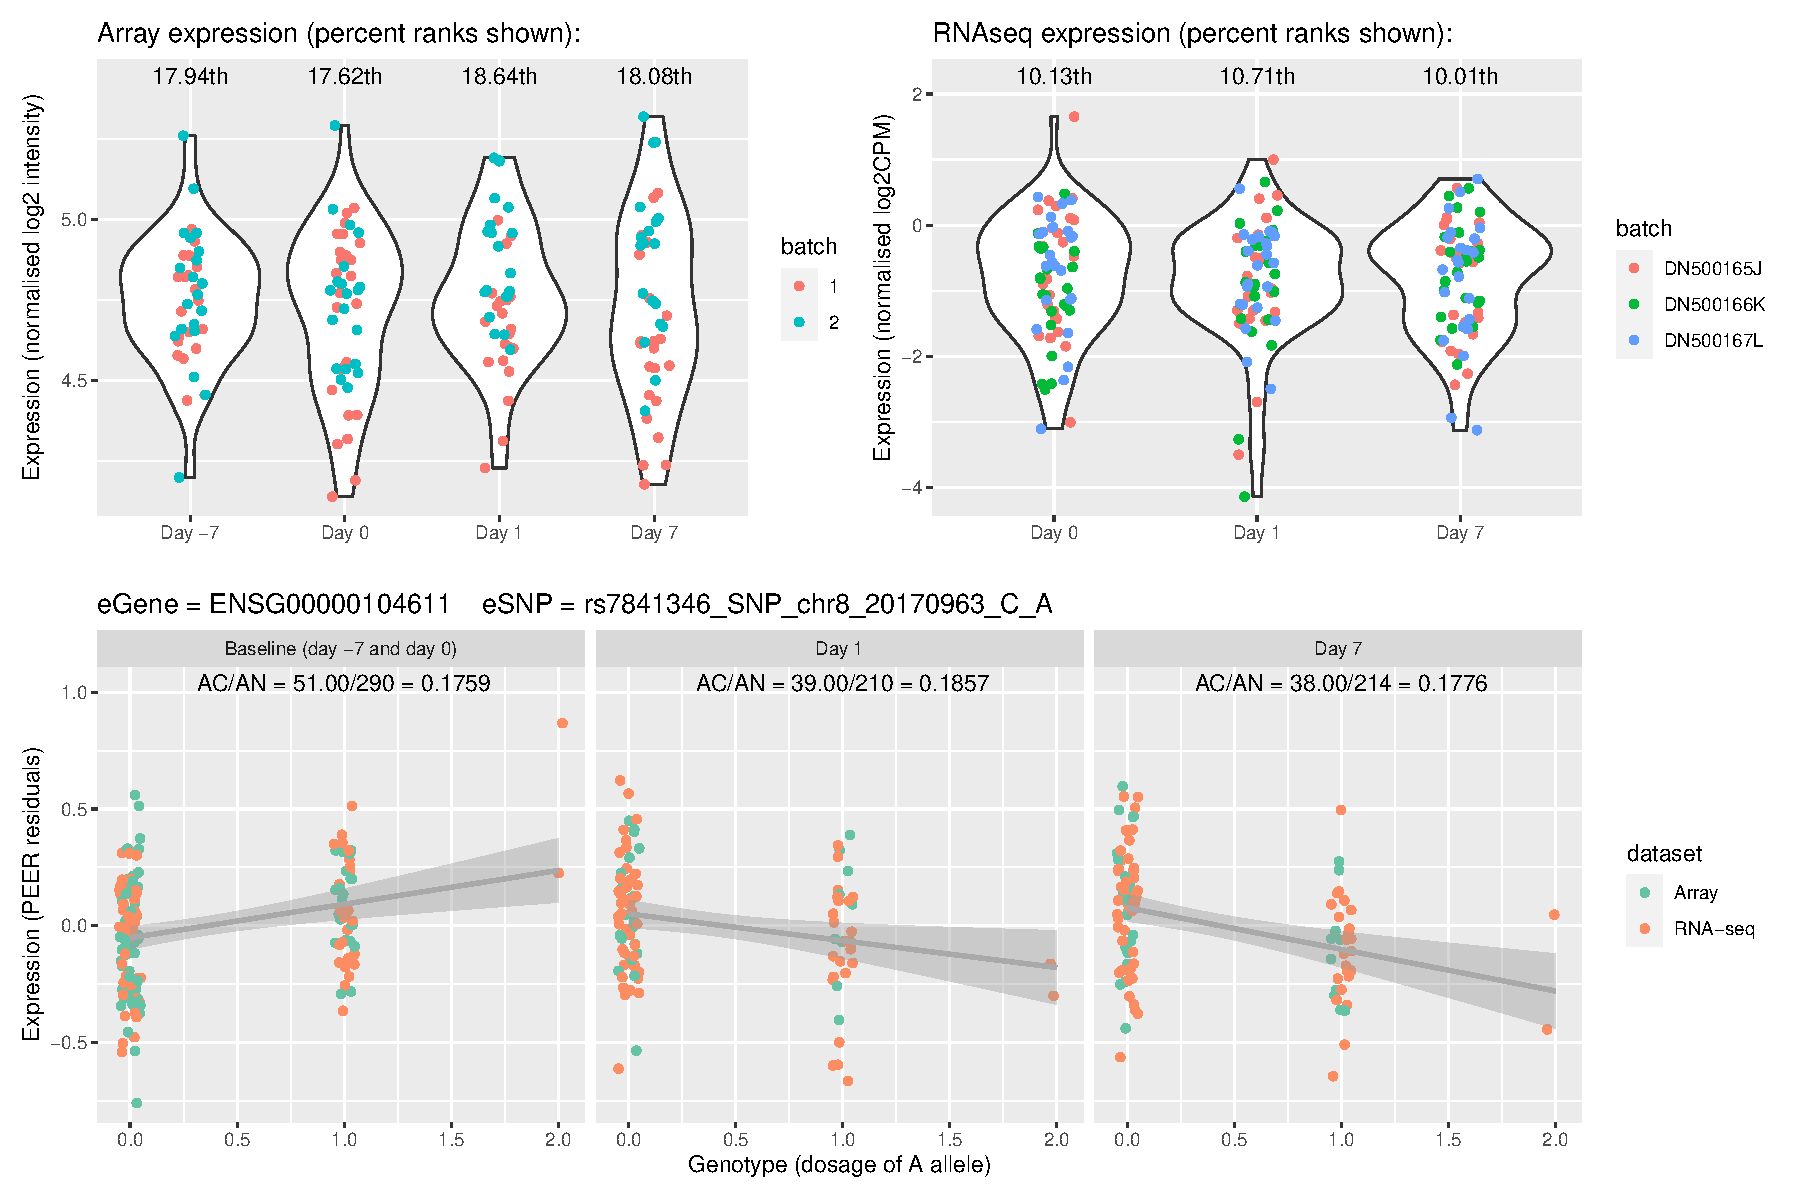
\includegraphics[width=1.0\textwidth,page=1]{mainmatter/figures/chapter_03/plot_dge_eqtl_genotypes.ENSG00000104611,rs7841346_SNP_chr8_20170963_C_A.pdf}
    \caption{
        \textbf{Expression and lead \gls{eQTL} of \gene{SH2D4A} over study timepoints.}
        Normalised array (top-left) and \gls{RNAseq} (top-right) expression before batch effect correction with ComBat.
        Bottom: \gls{eQTL} effects at each timepoint condition in the mega-analysis of array and \gls{RNAseq} data.
    }
    \label{fig:hird_eQTL_ploteQTL_SH2D4A}
\end{figure}

\subsubsection{Genotype by cell type interaction effects}

The presence of cell type-specific \gls{eQTL} effects combined with changes in cell abundance between timepoints was considered as an alternate explanation generating \glspl{reQTL}.
Even if an eGene is not differentially expressed on average in bulk expression data, 
the composition of cell types that are the source of that gene's transcripts can change.
\software{xCell} enrichment scores were used to approximate abundance of seven \gls{PBMC} cell types from the expression data.
After pruning highly correlated cell types to avoid multicollinearity, standardised scores for monocytes, \gls{NK} cells and plasma cells were tested for genotype interactions.
Within each timepoint, full \gls{eQTL} models including the genotype main effect, the three cell type abundance main effects, and three cell type-genotype interaction terms, were fit using \software{lme4qtl}, 
then compared to a nested model excluding the three interaction terms with a \gls{LRT}.
% The nested model has the same form as the within-timepoint models used in the main \gls{reQTL} analyses.
Significant cell type interactions were detected at \num{16/1154} \glspl{reQTL}-gene pairs in at least one timepoint (\gls{BH} \gls{FDR} < 0.05).
Fifteen were significant in only one timepoint:
baseline (\gene{SLAMF8}, \gene{CSE1L}, \gene{MAST1}, \gene{DLGAP1}),
day 1 (\gene{ZNF519}, \gene{LPAR1}, \gene{ADCY3}, \gene{NAA20}, \gene{EPB41L5}),
or day 7 (\gene{APOL6}, \gene{ADAR}, \gene{ADAM17}, \gene{UHRF2}, \gene{MST1}, \gene{CUL1}).
% \gene{SMDT1} at both d0 and d7

% $\chi^2(3) = \num{26.290769}$,
For \gene{ADCY3} at day 1 (full vs. nested \gls{FDR} = \num{9.539518e-05}),
although the genotype effect was \num{0.255954767} (SE = \num{0.03339378}) in the nested model,
% 0.35803609 \pm 0.05570632 limix
% 0.13549316 \pm 0.03266963 mashr
the estimate in the full model was \num{-0.007216815} (\num{0.06656115});
with the three cell type-genotype interaction term estimates being
\num{0.212978154} (\num{0.04897962}) for monocytes,
\num{-0.009195402} (\num{0.04470412}) for \gls{NK} cells,
and \num{0.016151511} (\num{0.06632921}) for plasma cells.
The small magnitude of the genotype main effect in the full model compared to the nested model suggests the \gls{eQTL} effect is driven largely by the monocyte score (or a cell type that is highly correlated with monocyte score in \cref{fig:hird_xCell_correlationMatrix}).
In the case where the monocyte score is zero (representing an average abundance across samples, as scores are standardised), the effect of increasing genotype dosage on \gene{ADCY3} expression is minimal.
\cref{fig:hird_reQTL_ADCY3_vs_monocyte_baseline,fig:hird_reQTL_ADCY3_vs_monocyte_day1} illustrate this effect.
Monocyte abundance has no effect on expression at baseline, 
increases after vaccination, and modifies the effect of genotype on expression at day 1.
It is feasible that the mechanism generating \gls{reQTL} at the remainder of these genes also involve cell type-specific \gls{eQTL} effects, 
but unlike at \gene{ADCY3}, 
I have not yet examined which of the three cell abundance scores have the greatest contribution.

\begin{figure}
    \centering
    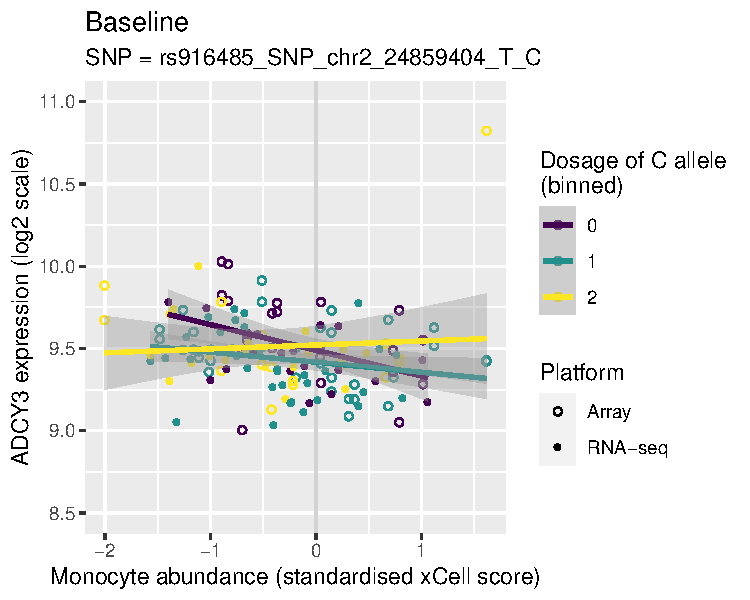
\includegraphics[width=1.0\textwidth,page=1]{mainmatter/figures/chapter_03/lme4qtl.ENSG00000138031_Monocyte_baseline.pdf}
    \caption{
        \textbf{Effect of estimated monocyte abundance on \gene{ADCY3} expression at baseline, stratified by genotype at a day 1 \gene{ADCY3} \gls{reQTL}.}
    }
    \label{fig:hird_reQTL_ADCY3_vs_monocyte_baseline}
\end{figure}

\begin{figure}
    \centering
    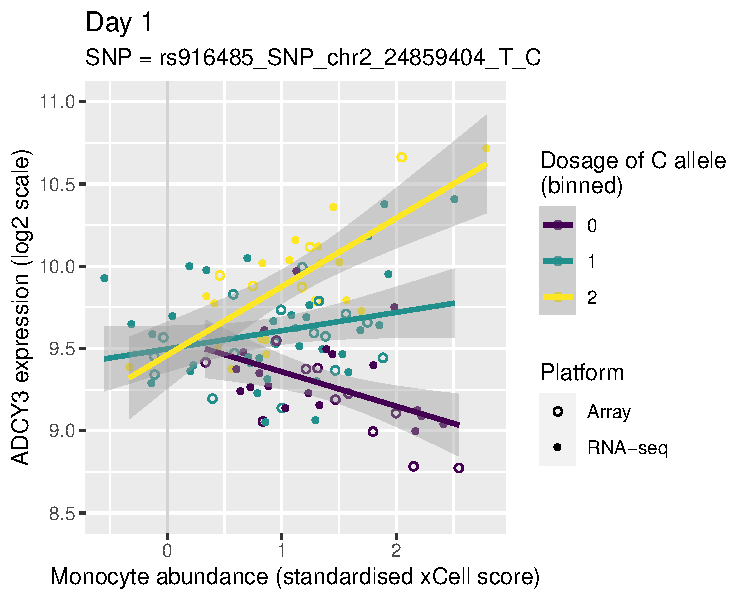
\includegraphics[width=1.0\textwidth,page=1]{mainmatter/figures/chapter_03/lme4qtl.ENSG00000138031_Monocyte_day1.pdf}
    \caption{
        \textbf{Effect of estimated monocyte abundance on \gene{ADCY3} expression at day 1, stratified by genotype at a day 1 \gene{ADCY3} \gls{reQTL}.}
    }
    \label{fig:hird_reQTL_ADCY3_vs_monocyte_day1}
\end{figure}

% \subsection{Genotype by platform interaction effects}
%
% pull platform interaction in as a filter
%
% potential problems with mega discussed b4
% - platform fx
% - Using a fixed effect assumes mean diff between rnaseq and array and forces the slope to the average.
% - lme4qtl interactions with bonferroni
% - Perhaps using platform specific effects as a filter for reQTLs.
%
% TODO Need to consider Nikos' comment that there are too many (1069/13570 significant BH FDR) genotype-platform interactions to use mega-analysis. Consider filtering.

\subsubsection{Colocalisation with external QTL datasets at the \gene{ADCY3} locus}

The day 1 \gene{ADCY3} \gls{reQTL} is of particular interest,
as \gls{reQTL} were also found for \gene{ADCY3} in blood approximately 1 day after stimulation with \gls{TIV} \autocite{franco2013IntegrativeGenomicAnalysis}, rhinovirus \autocite{caliskan2015HostGeneticVariation}, and \textit{Mycobacterium leprae} \autocite{manry2017DecipheringGeneticControl}.
% NOTE: Also in obesity and T2D
The locus that contains the \gene{ADCY3} \gls{reQTL} has also been implicated in disease risk for \glspl{IMID} such as \gls{IBD} \autocite{delange2017GenomewideAssociationStudy},
and \gene{ADCY3} expression in immune cells in gut mucosa has been suggested to contribute to \gls{CD} risk (a subtype of \gls{IBD}) \autocite{marigorta2017TranscriptionalRiskScores}.
Aside from monocytes, \gene{ADCY3} is expressed in a wide range of immune cells---CD4\textsuperscript{+} T cells, CD8\textsuperscript{+} T cells, B cells, and \gls{NK} cells (\cref{fig:hird_eQTL_ADCY3_expression_DICE}).
Identifying cell type-dependent \gls{eQTL} through genotype-cell type abundance interaction terms cannot distinguish between cell types with highly correlated abundances \autocite{kim-hellmuth2020CellTypeSpecific}.
The high contributions to the same \gls{PC} for monocyte, CD4\textsuperscript{+} T cell, and CD8\textsuperscript{+} T cell xCell scores in the \gls{PCA} xCell scores indicates cell types with high \gene{ADCY3} expression are indeed correlated in \gls{HIRD} (\cref{fig:hird_xCell_cos2}).
Given the locus is associated with response to a wide range of immune stimuli, and also an \gls{IMID},
I conducted colocalisation analysis to test if shared causal variants 
may be driving these associations and to determine which of the correlated cell types expressing \gene{ADCY3} are mostly likely responsible.

\begin{figure}
    \centering
    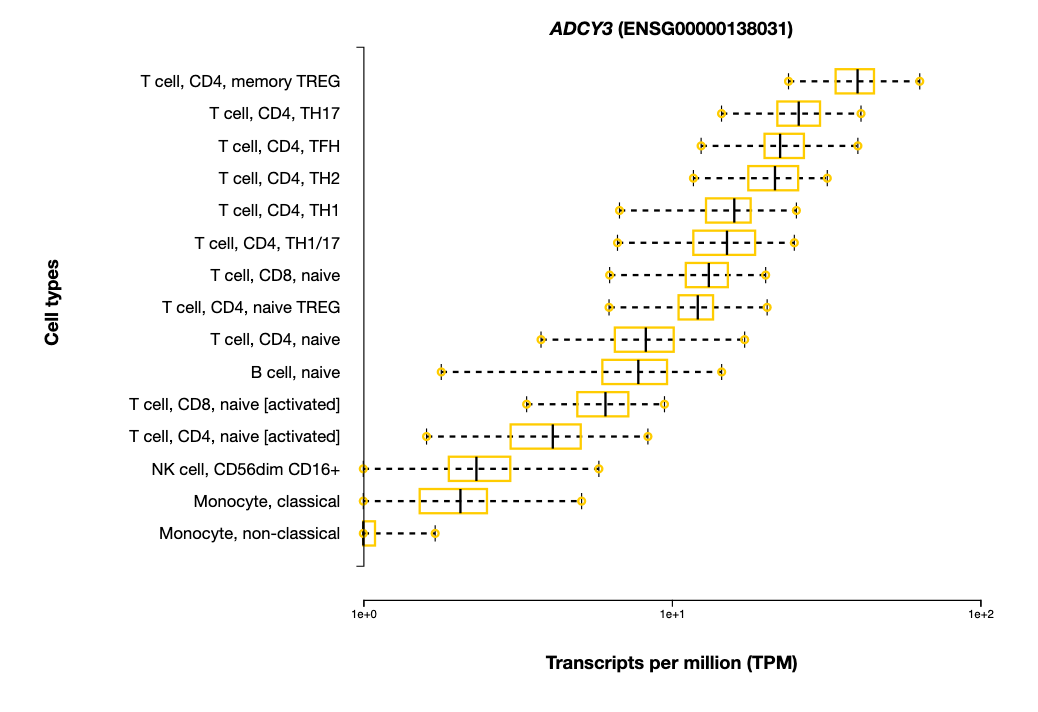
\includegraphics[width=1.0\textwidth,page=1]{mainmatter/figures/chapter_03/ADCY3_expression.png}
    \caption{
        \textbf{Expression of \gene{ADCY3} in sorted immune cell subsets.}
        \textcite{schmiedel2018ImpactGeneticPolymorphisms}, 
        \textit{DICE (database of immune cell expression, expression quantitative trait loci, and epigenomics}, 
        \url{https://dice-database.org/genes/ADCY3}, accessed Nov 2020.
    }
    \label{fig:hird_eQTL_ADCY3_expression_DICE}
\end{figure}

% rs916485_SNP_chr2_24859404_T_C
In a \SI{\pm 500}{\mega\bp} window around the lead \gls{reQTL} variant rs916485,
I performed Bayesian multi-trait colocalisation (\software{HyPrColoc} \autocite{foley2019FastEfficientColocalization}) of
the three per-timepoint \gene{ADCY3} \gls{eQTL} summary statistics with external datasets:
\gene{ADCY3} \gls{eQTL} from 15 sorted immune cell populations from \textcite{schmiedel2018ImpactGeneticPolymorphisms},
monocyte count \gls{QTL} from \textcite{astle2016AllelicLandscapeHuman},
and \gls{IBD} \gls{GWAS} from \textcite{delange2017GenomewideAssociationStudy}.
There were 1054 variants present in all 20 sets of summary statistics.

\software{HyPrColoc} identifies clusters of traits that colocalise at different causal variants in the locus.
As Bayesian colocalisation can be sensitive to the choice of priors,
I performed a sensitivity analysis iterating over configurations of priors and other algorithm parameters, ranging from default to more stringent parameter values.
Two stable clusters were identified across 100 configurations of parameters (\cref{fig:hird_reQTL_coloc_ADCY3_sensitivityPlotCustom}).
A set of three traits---\gene{ADCY3} expression in \gls{HIRD} day 1 and in naive classical and non-classical monocytes---clustered in \textapprox{\SI{65}{\percent}} of tested configurations.
A set of nine traits---\gls{IBD} and expression in eight naive and memory CD4+ T cell subsets---clustered in \textapprox{\SI{90}{\percent}} of tested configurations.
The remaining traits did not robustly cluster with any other traits over the tested configurations,
except for the rare inclusion of \gls{HIRD} baseline \gene{ADCY3} expression into the larger cluster for less stringent configurations.

% ADCY3 TSS is at 24919839, rev strand
%
% posterior_prob regional_prob candidate_snp posterior_explained_by_snp
%
% IBD T cell
% 0.9778        1.0000  2_24935139_C                          1
% rs713586 2:24935139 T C 
% 15300 upstream
%
% HIRD monocyte
% 0.9424        1.0000  2_24874083_C                          1
% rs7567997 2:24874083 T C
% 45756 downstream
%
The value of \software{prior.2} (the probability that a variant associated with at least one trait is not associated with any additional traits) was subsequently set to 0.99 (default = 0.98) to increase stringency, preventing clustering of baseline \gls{HIRD} expression with T cell and \gls{IBD}.
The values of other priors and algorithm parameters were left at their defaults, producing the final clustering shown in \cref{fig:hird_reQTL_coloc_ADCY3_locusPlot}.
Under this configuration, the posterior probability that all traits in the cluster share a causal variant was \num{0.9778} for the larger cluster (CD4\textsuperscript{+} T cell expression and \gls{IBD}), 
and \num{0.9424} for the smaller cluster (\gls{HIRD} day 1 and monocyte expression).
Distinct candidate causal variants were proposed for each cluster.
For the larger cluster, rs713586, a variant \SI{15}{\kilo\bp} upstream of the canonical \gene{ADCY3} \gls{TSS};
and for the smaller cluster, rs7567997, an intronic variant \SI{45}{\kilo\bp} downstream of the \gls{TSS}.
In both cases, the variant explained all of the posterior probability for the cluster, 
but as the analysis is restricted to the 1054 variants present in all datasets, there is ample chance the true causal variants were not included.
When it comes to fine mapping, it will be more appropriate to perform it in the dataset with the densest genotyping.

\begin{figure}
    \centering
    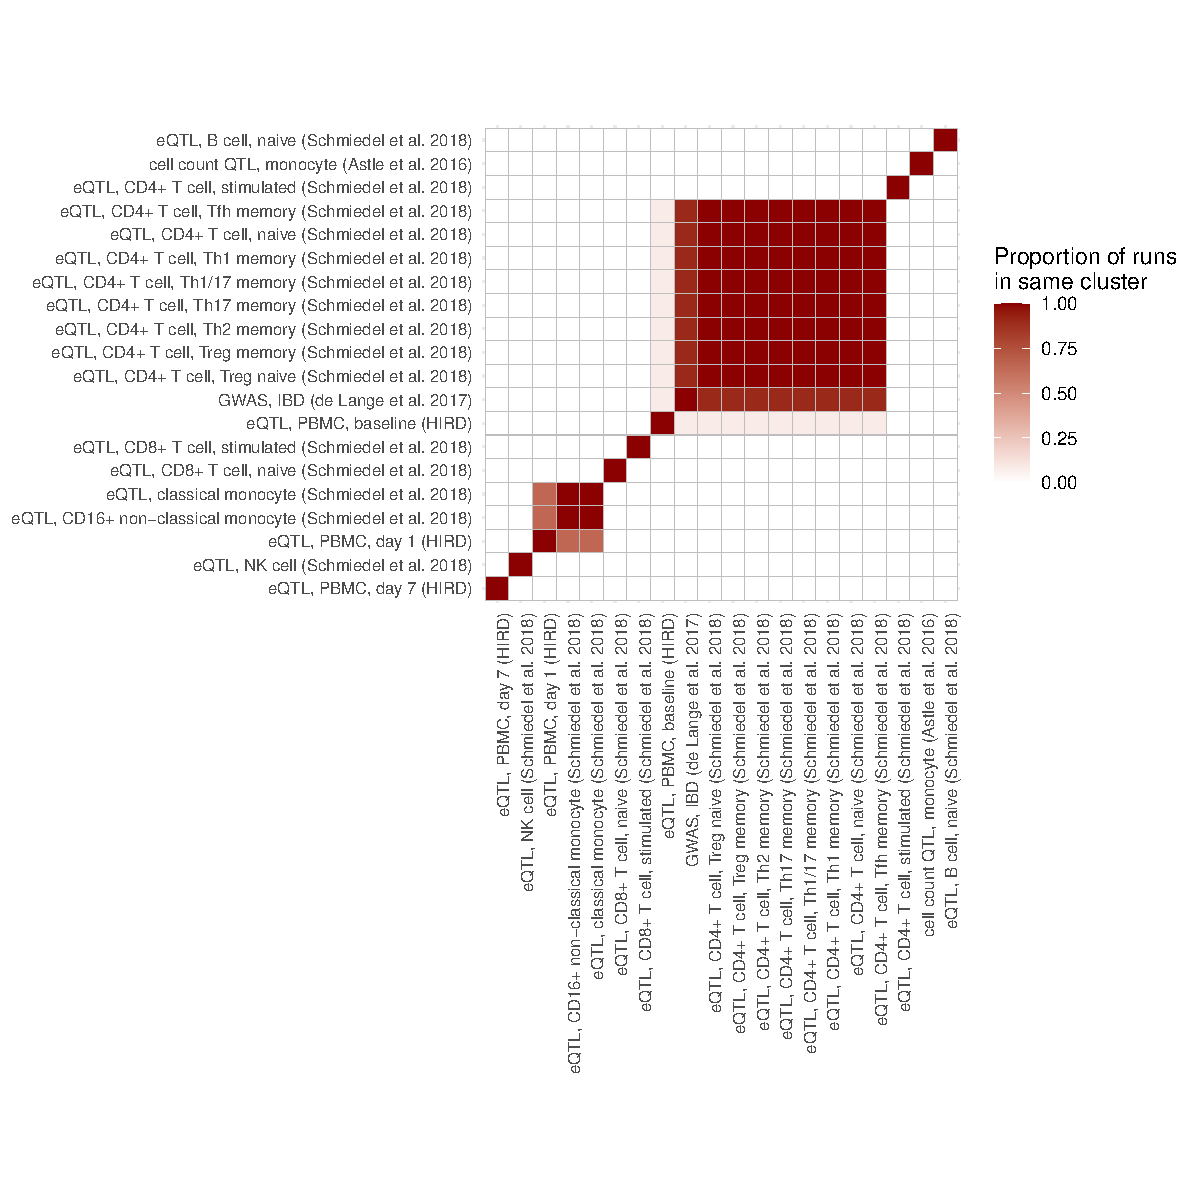
\includegraphics[width=1.0\textwidth,page=1]{mainmatter/figures/chapter_03/perform_coloc.gene_ENSG00000138031.sensitivityPlot_custom.pdf}
    \caption{
        \textbf{Sensitivity analysis for multi-trait colocalisation at the \gene{ADCY3} locus.}
        Colocalisation done using \software{HyPrColoc} \autocite{foley2019FastEfficientColocalization} in a 500 Kb window around the lead variant for the day 1 \gene{ADCY3} \gls{reQTL} in \gls{HIRD} for trait datasets described in \cref{subsec:hird_reQTL_coloc}.
        Heatmap shows the proportion of configurations in which two traits colocalise in the same cluster over 100 configurations of algorithm parameters
        \software{reg.thresh}, \software{align.thresh}, and \software{prior.2} (range of values listed in \cref{subsec:hird_reQTL_coloc}).
        \software{prior.1} set at \num{1e-4} (default).
        Rows and columns hierarchically-clustered.
    }
    \label{fig:hird_reQTL_coloc_ADCY3_sensitivityPlotCustom}
\end{figure}

\begin{figure}
    \centering
    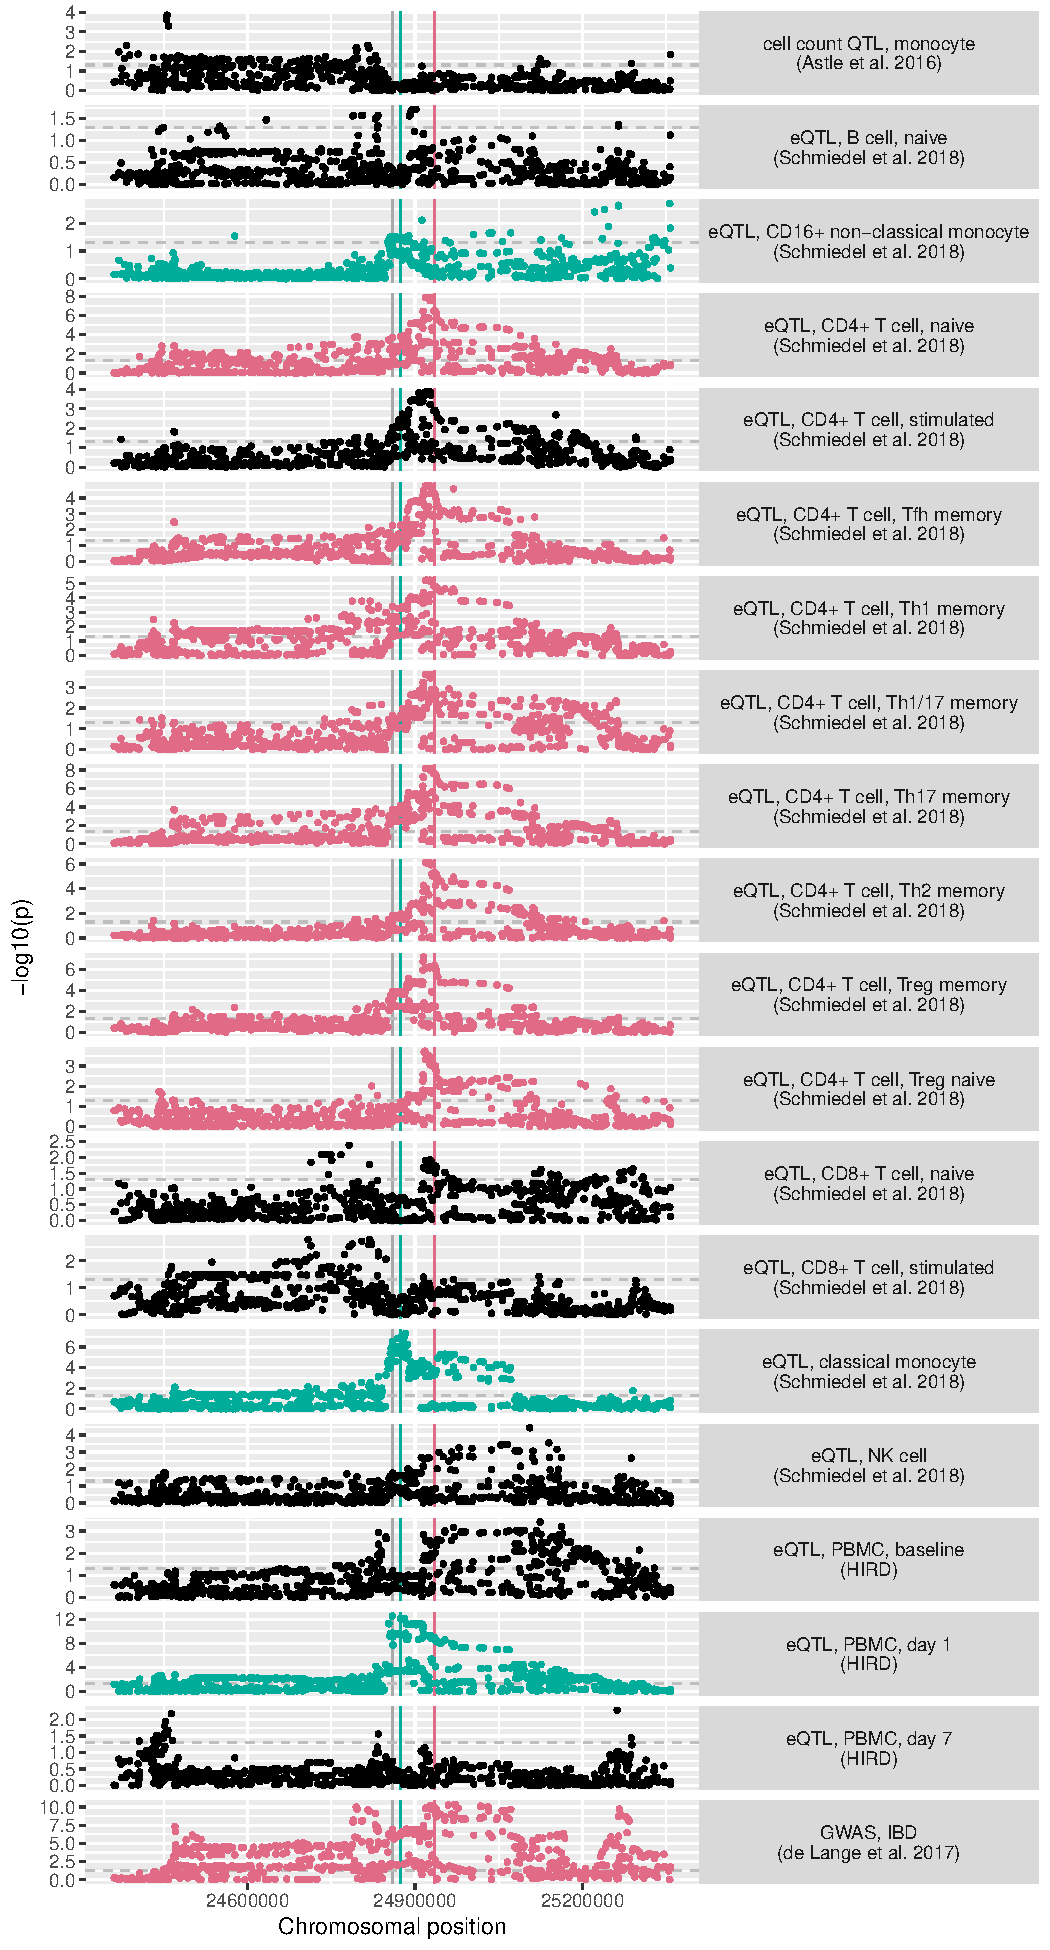
\includegraphics[width=1.0\textwidth,page=1]{mainmatter/figures/chapter_03/perform_coloc.gene_ENSG00000138031.locusPlot.pdf}
    \caption{
        \textbf{Multi-trait colocalisation at the \gene{ADCY3} locus.}
        Colocalisation done using \software{HyPrColoc} \autocite{foley2019FastEfficientColocalization} in a 500 Kb window around the lead variant for the day 1 \gene{ADCY3} \gls{reQTL} in \gls{HIRD} (vertical grey line).
        Traits are monocyte cell count (\textcite{astle2016AllelicLandscapeHuman}), \gene{ADCY3} expression in sorted immune cell subsets (\textcite{schmiedel2018ImpactGeneticPolymorphisms}), \gene{ADCY3} expression in \gls{HIRD} timepoints, and \gls{IBD} (\textcite{delange2017GenomewideAssociationStudy}).
        Locus plots show summary statistics for 1054 variants present in all datasets.
        Traits in red and green represent two distinct clusters each hypothesised to be driven by a shared causal variant (vertical red and green lines).
        Non-colocalising traits are shown in black.
        Horizontal dashed line shows p = 0.05.
        Default values for priors and algorithm parameters used, except \software{prior.2} = 0.99.
    }
    \label{fig:hird_reQTL_coloc_ADCY3_locusPlot}
\end{figure}

Nevertheless, the two main clusters being distinct from one another, and from non-colocalising traits across many configurations,
still supports the existence of distinct causal variants, even if they may be unobserved.
For \gls{HIRD} day 1 expression of \gene{ADCY3}, the more relevant cell type appears to be monocytes, not a correlated cell type like CD4\textsuperscript{+} T cells---and vice versa for \gls{IBD}.
The clustering was robust despite the data containing no stimulated monocyte subsets.
This \gls{eQTL} effect is readily observable at baseline, and appears to be more significant in naive classical than non-classical monocytes in the \textcite{schmiedel2018ImpactGeneticPolymorphisms} data (\cref{fig:hird_reQTL_coloc_ADCY3_locusPlot}).
No colocalisation with blood monocyte count was observed, 
so the \gls{reQTL} does not appear to affect monocyte abundance in general.
I believe a variant that affects ability to increase monocyte counts post-vaccination can also be ruled out,
as in that case the effect of genotype on expression is entirely mediated through the effect of genotype on monocyte abundance,
so having cell abundances as covariates in the regression should eliminate that effect.
Thus I hypothesise that a plausible mechanism generating the day 1 \gls{reQTL} signal in \gls{HIRD}
is an increase in abundance of classical monocytes at day 1 post-vaccination,
increasing the proportion of \gene{ADCY3} transcripts in the bulk data originating from monocytes,
thus making an \gls{eQTL} specific to monocytes--not just stimulated monocytes---more readily detectable.
This is the scenario where monocyte abundance modifies the effect of genotype on expression.

\section{Discussion}

Just as vaccination was found to induce extensive changes in the transcriptome
in \cref{ch:hird_DGE},
it also induces changes in the regulatory architecture of gene expression.
In a mega-analysis of array and \gls{RNAseq} datasets,
\textit{cis}-\gls{eQTL} were detected for \percentage{0.5075166} (\num{6887/13570}) of genes in at least one timepoint,
and the majority replicated in the much larger GTEx whole blood dataset.
This is a substantial eGene rate given the modest per-timepoint sample size in \gls{HIRD}, reflecting the gain in effective sample size from joint mapping over multiple conditions.
% Each method for determining reQTL has its own biases.
% Even in a joint mapping framework, defining \gls{reQTL} by set significance thresholds, or change in the amount of expression variation explained, will miss classifying equal but opposite effect sizes.
Defining reQTL from a significant difference in beta of the same \gls{eQTL} between timepoints,
\num{1154/6887} (\percentage{0.1675621}) of lead \gls{eQTL} were classified as \gls{reQTL}.
This is comparable to estimates of \SIrange{3}{18}{\%} \gls{reQTL} between monocytes in different stimulation conditions by \textcite{kim-hellmuth2017GeneticRegulatoryEffects} who also used a beta comparison approach.
The method is relatively stringent at calling \gls{reQTL},
avoiding both threshold effects where significant and non-significant \gls{eQTL} may have very similar betas,
and discovery power biases caused by sample size differences between conditions.
Indeed, had \gls{reQTL} been called by significance alone, 1427 \gls{reQTL} would have been detected just at baseline, the timepoint with the largest sample size in \gls{HIRD}.
There is a growing consensus in the literature that most \gls{eQTL} are shared between conditions such as tissue and cell-type \autocite{ongen2017EstimatingCausalTissues,urbut2018FlexibleStatisticalMethods,kim-hellmuth2020CellTypeSpecific,umans2020WhereAreDiseaseAssociated},
and that high estimates of 50\% or more condition-specificity based on significance thresholds (e.g. \autocite{ackermann2013ImpactNaturalGenetic}) are overestimated.
A counter-argument is that many studies overestimate sharing by calling condition-specific effects in \gls{LD} as shared \autocite{umans2020WhereAreDiseaseAssociated}.
Here I compared the same gene-tag \gls{SNP} pair across timepoints,
but distinct causal and condition-specific variants may be tagged in such a way that the effect size of the tag \gls{SNP} ends up similar---multi-trait colocalisation would be required to truly confirm a shared \gls{eQTL}.

Gene set enrichment analyses to identify shared biological processes among target genes for \gls{reQTL} were generally uninformative.
Genes targeted by \gls{reQTL} that explained more variation in expression post-vaccination were enriched for immune activation, with weaker enrichments related to \gls{APC}.
This misses the full picture though, as many of the strongest \gls{reQTL} were those with opposite sign effects at baseline and post-vaccination not captured by changes in \gls{PVE}.
Prevalence of opposite sign effects between pairs of conditions has been previously described in multi-tissue studies;
in \textcite{fu2012UnravelingRegulatoryMechanisms}, the proportion of opposite sign effects among all reQTLs between five tissues was \percentage{0.044}.
In \gls{HIRD}, I found an unexpectedly high proportion:
39/819 (\percentage{0.04761905}) for day 1 \gls{reQTL},
and 211/1002 (\percentage{0.2105788}) for day 7 \gls{reQTL} (\cref{fig:hird_eQTL_zSharing_vs_TSSdist_mega}).
Given the larger global changes in expression vs. baseline at day 1 compared to
day 7 described in \cref{ch:hird_DGE}, 
the larger number of strong \glspl{reQTL} at day 7 was also unexpected.
The genes with these opposite sign effects were not significantly enriched in any of the gene sets or \glspl{BTM} I tested.
% In \autocite{mizuno2019BiologicalCharacterizationExpression}, the proportion of opposite sign effects as a percentage of all eGenes was \percentage{0.074} (48 tissues);
% in \gls{HIRD}, I find
% 39/6887 (\percentage{0.005662843}) at day 1,
% and 211/6887 (\percentage{0.03063743}) at day 7.

Post-vaccination \gls{DGE} was considered as a mechanism that might generate \gls{reQTL}.
As in \textcite{kim-hellmuth2017GeneticRegulatoryEffects, davenport2018DiscoveringVivoCytokineeQTL}, the overlap between \gls{DGE} and genes with reQTL in \gls{HIRD} was poor.
Only at day 7 were \gls{reQTL} more likely to be differentially expressed than genes without reQTL, specifically when restricting the analysis to eGenes.
Those day 7 \gls{reQTL} that were also upregulated at day 7 were enriched in cell cycle Gene Ontology sets, but it is unclear how this may lead to generation of opposite effects, and the enrichment may largely be driven by the \gls{DGE} signal rather than the \gls{reQTL} one.
To define genes important to \gls{TIV} response,
\textcite{franco2013IntegrativeGenomicAnalysis} made heavy use of the overlap of \gls{DGE} and \gls{eQTL}, followed by gene set enrichment.
Unfortunately, their overlap criteria before enrichment covered genes with either \gls{DGE} \emph{or} \gls{reQTL}, so it is difficult to assess 
which contributed more to their significant enrichments in the antigen presentation pathway.
% 20 genes from Franco
% 12/17 DGE replicated
% 14/17 eGenes replicated, none were reQTL
% TODO dge is coupled to reqtl, if you do an enrichment of dge+reqtl overlap genes, likely their enrichment is driven by DGE signal
As noted by \textcite{davenport2018DiscoveringVivoCytokineeQTL,cuomo2020SinglecellRNAsequencingDifferentiating}, 
it may be that \gls{DGE} and \gls{reQTL} are generated by different mechanisms, and focusing on the overlap is an unnecessarily narrow view. 

An unappealing thought is that opposite sign effects are enriched in false positives, especially as they seem to show no positional enrichment near the \gls{TSS}.
While it is known that stimulation-specific \gls{reQTL} are more distal than baseline eQTL \autocite{fairfax2014InnateImmuneActivity}, the \gls{HIRD} reQTL are evenly spread across the cis- window.
Some reQTL may be statistical artifacts of the shrinkage of effects by \software{mashr}.
Small and opposite effects generated by noise may be frequent enough for \software{mashr} to consider them a \enquote{pattern} of effects.
This might explain the clear separation of the distribution of z-statistics for difference in beta between \gls{reQTL} and shared eQTLs.
Conversely, it may be that small and opposite effects are more prevalent than expected, and combination of \software{mashr} and the difference in betas test is the best framework for detecting them.
To confirm either way, it may be necessary to repeat the \gls{reQTL} calling without the influence of \software{mashr} shrinkage in a different modelling framework,
such as a timepoint-genotype interaction term \autocite{davenport2018DiscoveringVivoCytokineeQTL}.
A complementary approach for validating these opposite sign \gls{reQTL} using the existing \gls{RNAseq} data might be within-individual \gls{ASE} (e.g. RASQUAL \autocite{kumasaka2016FinemappingCellularQTLs}, PLASMA \autocite{wang2020AlleleSpecificQTLFine}),
which can be performed with the same data types as \gls{eQTL} mapping,
and where one would expect true opposite sign \gls{reQTL} effects would also be recapitulated as opposite directions of allelic expression imbalance.
\gls{ASE} may also provide more interpretable effect sizes than \gls{eQTL} betas \autocite{mohammadi2017QuantifyingRegulatoryEffect},
for purposes such as clustering effect sizes to determine patterns of effects across timepoints \autocite{cuomo2020SinglecellRNAsequencingDifferentiating}.

At least one \gls{reQTL} signal was plausibly not a false positive.
The strongest \gls{reQTL} detected at day 1 was for \gene{ADCY3}, a membrane-bound enzyme that catalyses the conversion of ATP to the second messenger cAMP \autocite{wu2016AdenylateCyclaseNew}.
% During the process of ‘tolerance/immunoparalysis’, a common complication of severe sepsis, monocytes enter a refractory functional state, characterized by the incapacity to produce proinflammatory cytokines and decreased HLA-DR expression (9). Tolerance can be mimicked in vitro and in vivo by challenging the cells with endotoxins such as LPS: after an initial stimulation phase, cells enter a state of long-term immunotolerance. In contrast, other infections or vaccinations (e.g. Candida albicans infection, Bacille Calmette-Guerin (BCG) or measles vaccination) increase the long-term responsiveness of monocytes to microbial stimuli, a state termed ‘trained immunity’ which confers resistance to secondary infections (10–14).
\gene{ADCY3} is upregulated after the differentiation of monocytes induced by beta-glucan,
into macrophages in a state of trained immunity---a state in which they are more responsive to future immune stimuli \autocite{saeed2014EpigeneticProgrammingMonocytetomacrophage}.
\Glspl{GWAS} have implicated the \gene{ADCY3} locus for diseases such as obesity \autocite{wu2016AdenylateCyclaseNew} and \gls{IBD} \autocite{delange2017GenomewideAssociationStudy}.
\gene{ADCY3} has also been identified as a post-stimulation \gls{reQTL} in other studies involving stimulated blood immune cells:
% In fact, six (SLFN5, ARL5B, SPTLC2, IRF5, ADCY3, CCDC146) of the 38 genes
% implicated in our reQTL mapping were also identified in a recent reQTL mapping
% study for Escherichia coli lipopolysaccharide, influenza, and interferon-β in
% dendritic cells [35].
in \gls{PBMC} 24h after \textit{in vitro} infection with rhinovirus \autocite{caliskan2015HostGeneticVariation},
in whole blood \textit{in vivo} day 1 after vaccination with seasonal \gls{TIV} \autocite{franco2013IntegrativeGenomicAnalysis},
% Examples of three reQTL among genes found only in M. leprae sonicate stimulated
% cells or non-stimulated cells. For each gene ((A) ADCY3, (B) DNAAF1 and (C)
% ZNF517): the left panel corresponds to the expression of the gene in
% non-stimulated cells while the right panel depicts expression of the gene in
% stimulated cells. The gene identity is indicated above each pair of graphs. The
% gene expression level in log2 scale (y-axis) is plotted for each genotype
% (x-axis). Of note, reQTL for the ADCY3 and DNAAF1 genes have been found by
% other studies using distinct pathogens or molecules as stimuli, while the reQTL
% for ZNF517 is a newly identified reQTL [21, 22, 24, 26]. ADCY3 is among the
% most upregulated genes after stimulation with M. leprae antigens and has been
% identified as part of the T1R gene set signature identified by Orlova et al.
% [32]. The reQTL for DNAAF1 displays the strongest p value among the reQTL we
% identified.
and in whole blood after \textit{in vitro} stimulation with \text{M. leprae antigen} for 26-32 h \autocite{manry2017DecipheringGeneticControl}.
% TODO:
% Aside from \gene{ADCY3}, I also see \autocite{caliskan2015HostGeneticVariation} a day 1 reQTL at \gene{SLFN5} (PVE increase from \num{0.27048709} to \num{3.386358e-01}, p diff = \num{4.882379e-02}). , but no upreg
%
Given the diversity of stimulations and tissue types, the effect is likely a consequence of general immune activation, rather than a Pandemrix-specific response.

The strength of the \gene{ADCY3} \gls{reQTL} at day 1 was found to be modified by xCell estimates of monocyte abundance. 
% Changes in relative abundances for many cell types occur in the bulk PBMC samples after vaccination.
% I accounted for the effect of abundance on mean expression including xCell scores and PEER factors as fixed effects in the model,
% and also considered the effect of abundance on the genotype effect using interaction terms between xCell scores and genotype.
% Due to the modest sample size, and computational requirements for \software{lme4qtl},
% I focused only whether reQTLs that have a detectable main effect may be driven by cell type interactions,
% testing only for interactions at significant lead \gls{reQTL},
%
The xCell scores are imperfect.
Compared to FACS measurements in a cohort subset, the xCell scores were only weakly correlated, and the signatures used by xCell may be less accurate after vaccine stimulation.
Fortunately, statistical colocalisation confirms that the day 1 reQTL signal identified for \gene{ADCY3} is likely to be a monocyte-specific effect---and independent to the IBD signal in the locus, which colocalises with CD4 T cell eQTL datasets.
The proportion of monocytes in the \gls{PBMC} compartment increases at day 1, supported by both FACS \autocite{sobolev2016AdjuvantedInfluenzaH1N1Vaccination} measurements, and an increase in monocyte xCell score.
Expression of \gene{ADCY3} is not monocyte-specific: despite the increase in monocyte proportion, no upregulation was observed at day 1.
Colocalisation was also not restricted to stimulated monocytes.
The probable mechanism is an increased proportion of the bulk sample taken up by monocytes at day 1 providing more monocyte-derived \gene{ADCY3} transcripts,
rather than a upregulation-driven increase in detection power,
or a vaccine-induced activation of the locus at day 1.
Although multi-trait colocalisation proved to be the crucial piece of evidence suggesting the effect is not related to T cells,
only 15 immune cell types were included in the analysis, so it is possible the reQTL is not entirely monocyte specific.
%
% TODO: HyPrColoc assumes non-independent studies with overlapping samples have same LD
% astle: european
% hird: 70% eu
% dice is multi ethnic san diego, 50% white eu
% fairfax: european 
% gtex: largely eu before v8
%
% TODO: multiple causal variant methods still developing \autocite{wallace2020ElicitingPriorsRelaxing}

Overall, cell type interactions were only detected at 16/1154 reQTLs.
% the genotype effect was detected to interact with abundance of one or more of the tested cell types (or a correlated cell type).
Although power to detect significant interactions is lower than power to detect main effects,
not helped by the unclear reliability of xCell scores,
it is still likely that mechanisms other than shifts in cell abundance underlie a large number of the detected reQTLs.
% A pressing question remains: what molecular mechanisms underlie the \gene{ADCY3} \gls{reQTL}, and indeed the remainder of the \glspl{reQTL}?
One type of mechanism by which cis-eQTL affect expression is through their impact on \gls{TF} binding affinity to motifs in promoters and enhancers \autocite{pai2015GeneticMechanisticBasis}.
Immune cells, including monocytes, are heavily regulated by cell type-specific \glspl{TF} \autocite{choudhury2016IdentifyingCellTypeSpecific}.
Cell type-specific expression of different \glspl{TF} have been proposed as a model for explaining magnifying, dampening and opposite reQTL effects;
for example, opposite effects can result from \glspl{TF} regulating the same gene, that are activating in one cell type and suppressive in another \autocite{fu2012UnravelingRegulatoryMechanisms}.
There is evidence that \gls{TF} activity is important for \textit{in vivo} immune reQTL:
\textcite{caliskan2015HostGeneticVariation} found rhinovirus reQTLs in \glspl{PBMC} were enriched in ENCODE ChIP-seq peaks for the \glspl{TF} \gene{STAT1} and \gene{STAT2},
and \textcite{davenport2018DiscoveringVivoCytokineeQTL} found interferon and anti-IL6 drug reQTLs likely disrupt \gene{ISRE} and \gene{IRF4} binding motifs.
Rather than condition-specific expression of the eGene, what may be condition-specific is the expression of \glspl{TF} whose activity is affected by the reQTL.
A genomic feature enrichment for TF binding sites and other regulatory elements like enhancer regions among HIRD reQTL variants could expose shared regulatory factors that explain subsets of the remaining reQTL.
This would also help evaluate if the even distribution of reQTL across the \textit{cis}- window is a cause for concern.

% \footnote{
%     A cursory scan of \gls{TF} motifs disrupted by the location of the fine-mapped \gene{ADCY3} reQTL intronic variant rs13407913 on \url{https://ccg.epfl.ch/snp2tfbs/snpviewer.php},
%     does indeed show several motifs (for NR2C2, HNF4A, HNF4G, NR2F1)
%     where the PWM score is higher for the ALT allele,
%     consistent with the direction of effect for the day 1 reQTL.
% }.
% introns can be TF bound 
%    https://journals.plos.org/plosone/article?id=10.1371/journal.pone.0046784
% Functional Annotations of SNP http://54.245.180.226/php_file/multiple.php?ID=rs13407913
%     SP1 is monocyte specific https://europepmc.org/article/med/28008225
%     and upreg at d1

Not only are the mechanisms at many detected reQTL unknown, there may be many more reQTL yet to detect.
Multiple independent eQTLs are present for a large fraction of eGenes \autocite{zeng2019ComprehensiveMultipleEQTL}.
As a single lead variant for reQTL assessment at each eGene was chosen based on significance across all conditions
to avoid \gls{reQTL} due to differential tagging efficiency,
I could not detect reQTL that are masked by a stronger shared eQTL at that gene.
This is not expected to be uncommon, as the effective sample size for shared eQTLs is usually large due to borrowing of information across conditions.
Secondary \gls{eQTL} signals tend to be weaker, more distal to the TSS, more likely to be enriched in enhancers rather than promoters, and importantly, more context-specific \autocite{kim-hellmuth2017GeneticRegulatoryEffects,vandiedonck2017GeneticAssociationMolecular,dobbyn2018LandscapeConditionalEQTL,rotival2019CharacterisingGeneticBasis}.
The proportion of genes with reQTL I detect based on only the lead signal likely represents a lower bound.
% Also see for conditional eQTL:
% https://academic.oup.com/hmg/article/26/8/1444/2970473
% https://journals.plos.org/plosgenetics/article?id=10.1371/journal.pgen.1003649
Step-wise conditional analyses at each lead variant will be required to uncover secondary associations, 
which then can be compared across timepoints in the same manner as the primary associations.
These associations, although weaker on average, may actually have more variable effects between timepoints.
I also do not consider \textit{trans}-\gls{eQTL} due to sample size, which are more likely to be condition specific than \textit{cis}-\gls{eQTL} \autocite{fairfax2012GeneticsGeneExpression,westra2014GenomeFunctionStudying,fairfax2014InnateImmuneActivity}.

Finally, I address the prospect that common genetic variation may explain some variation in antibody response to Pandemrix.
I have indirectly demonstrated genotype-dependent effects on expression response by identifying reQTLs with differing effect size between timepoints,
but have yet to determine resulting genotype-dependent differences in antibody phenotypes.
Some of the identified reQTLs will undoubtedly affect genes whose expression or post-vaccination expression change correlates with antibody response, 
but correlation is not transitive \autocite{langford2001PropertyBeingPositively},
so correlation of genotype with expression and expression with antibody response does not imply a correlation between genotype and antibody response.
Formal tests such as the CIT \autocite{millstein2009DisentanglingMolecularRelationships} will be required to distinguish mediation of genotype-antibody associations through gene expression from competing models.
\textcite{franco2013IntegrativeGenomicAnalysis} realised this, but concluded that they had insufficient power with a greater sample size and comparable study design to \gls{HIRD}.
The \gls{HIRD} cohort is also too small for a direct \gls{GWAS} of Pandemrix antibody response.
A suitable approach for prioritising reQTL that contribute to the antibody response to Pandemrix will be to leverage external genetic associations to similar phenotypes,
for example, colocalisation with existing GWAS summary statistics for antibody response to a similar type of adjuvanted, inactivated vaccine.
However, due to the number of possible generating mechanisms for bulk reQTL \textit{in vivo},
careful interpretation is required to glean any insight into the biology of the stimulation in question.
\cref{ch:discussion} will continue the discussion on the methodologies, experimental designs and upcoming technologies 
required to complement the \textit{in vivo} \gls{reQTL} design.


% Vaxcin (DEPRECATED)
% %
% Chapter 4
% DEPRECATED for multiPANTS chapter
%

\chapter{Response to live attenuated rotavirus vaccine (Rotarix) in Vietnamese infants}

\section{Introduction}

Summary 

Rotavirus vaccine efficacy is lower in LMICs than EU and NA.
Protective response to many vaccines is linked with genetic variation.
Hypothesis: difference in efficacy is due to differences in genetic variation.

Aim:
    identify genetic and transcriptomic markers associated with Rotarix protective response
    primary outcome will be Rotarix vaccine failure events 
    secondary outcomes will be antibody responses and genotypic characterization of the infection virus in Rotarix failure events

\subsection{The genetics of vaccine response in early life}

% The genetic regulation of infant immune responses to vaccination
% https://www.frontiersin.org/articles/10.3389/fimmu.2015.00018/full

\subsection{Rotavirus and rotarix in Vietnam}

\subsection{Known factors that affect rotavirus vaccine efficacy}

\section{Methods}

\subsection{RNA-seq data generation}

Stranded RNAseq AUTO with Globin Depletion (>47 samples) uses the NEB Ultra
II directional RNA library kit for the poly(A) pulldown, fragmentation, 1st and
2nd strand synthesis and the flowing cDNA library prep (with some minor tweaks
e.g. at during the PCR we use kapa HiFi not NEB's Q5 polymerase). Between the
poly (A) pulldown and the fragmentation we use a kapa globin depletion kit
(it's very similar to their riboerase kit but the rRNA probes are swapped for
globin ones).

\subsection{Genotyping}

We will also use the SNP data to accurately impute ABO blood groups and secretor status. 

\section{Results}

Transcriptomic response to rotavirus vaccination (pre- vs. post-, prime vs. boost dose, responders vs. non-responders)

Genetic contribution to transcriptomic response

\section{Discussion}


% multiPANTS
%
% Chapter 4
%
% multiPANTS DGE paper.

\chapter{Transcriptomic associations with anti-\glsfmtshort{TNF} drug response in \glsfmtlong{CD} patients}
\label{ch:multiPANTS}

\textit{
    The work presented in this chapter is a collaboration between 
    the Wellcome Sanger Institute,
    the Royal Devon and Exeter Hospital National Health Service (NHS) Foundation Trust,
    the University of Exeter,
    and AbbVie.
    I would like to thank 
    Dr Nicholas Kennedy and Dr Tariq Ahmad for kindly extending the opportunity to collaborate on the PANTS cohort;
    Mark Reppell, Samantha Lent, and others at AbbVie, for performing the RNA-seq library preparation and sequencing, initial quality control, alignment and quantification, and estimation of cell proportions from methylation data;
    Simeng Lin, for advice on the sample structure of PANTS;
    Aleksejs Sazonovs, for performing the genotype quality control;
    and other individuals in the Sanger-AbbVie-Exeter PANTS working group, for their feedback during our video conferences.
}

\section{Introduction}

\subsection{\Glsfmtlong{CD} and \glsfmtlong{IBD}}

% \1 <Description>
\gls{CD} is a chronic, inflammatory disease of the gastrointestinal tract, one of the two main forms of \gls{IBD}.
It is characterised by patchy inflammation, where lesions are interspersed with regions of normal mucosa. 
The lesions can be distributed anywhere in the gastrointestinal tract, and tend to be transmural, affecting all layers of the gut wall.
The second form, \gls{UC}, is characterised by continuous inflammation, with lesions that are superficial rather than transmural, and restricted to the colon \autocite{roda2020CrohnDisease}.
Whilst the two are distinct forms of \gls{IBD}, similarities in clinical presentation, available therapies, and genetic architecture mean \gls{CD} and \gls{UC} have often been studied together.
% This introduction will consider literature on \gls{CD}, \gls{UC}, and \gls{IBD}.
% The similarity is such that there is a subset of IBD-U patients with features of both CD and UC, and thus is difficult to classify as one or the other.
Both are \glspl{IMID}, a group of related diseases involving immune dysregulation of common inflammatory pathways.
Other \glspl{IMID} include \gls{T1D}, \gls{SLE}, \gls{RA}, \gls{MS}, and psoriasis \autocite{cotsapas2013ImmunemediatedDiseaseGenetics,david2018GeneticsImmunemediatedInflammatory}.

% \1 <Pathogenesis and host genetics>
Pathogenesis of \gls{CD} is not completely understood, but involves interaction of the immune system, environmental factors (e.g. smoking, stress, diet \autocite{ananthakrishnan2015EpidemiologyRiskFactors,roda2020CrohnDisease}), and gut microbial factors in a genetically-susceptible individual \autocite{desouza2016ImmunopathogenesisIBDCurrent}.
Since the seminal discovery by linkage analysis in 2001 that genetic variation in \gene{NOD2} was linked to \gls{CD} risk \autocite{todd2001TacklingCommonDisease},
much progress has been made in establishing the disease's genetic architecture.
% (NOD2 was the first gene to be genetically-associated with a common disease)
% The first IBD GWAS was in 2006 \url{https://www.ncbi.nlm.nih.gov/pmc/articles/PMC4410764/}
The most recent \gls{GWAS} studies catalogue over 240 risk loci for \gls{IBD} \autocite{delange2017GenomewideAssociationStudy}.
% \2 IBD GWAS identify loci that are in pathways that are drug targets \autocite{delange2017GenomewideAssociationStudy}
% \2 Genetic correlation between UC and CD is high \autocite{cotsapas2013ImmunemediatedDiseaseGenetics,david2018GeneticsImmunemediatedInflammatory}
Most associations are shared between \gls{CD} and \gls{UC}, but there is strong heterogeneity of effects at some loci, such as \gene{NOD2} being only associated to \gls{CD} risk \autocite{jostins2012HostMicrobeInteractions,liu2015AssociationAnalysesIdentify}.
% \2 Concordance rates amongst monozygotic twins are higher for CD (~50\%) than for UC (\textapprox{15}\%) suggesting a greater heritable component \autocite{roda2020CrohnDisease}

% \1 <Epidemiology and burden>
\gls{CD} has historically been considered a disease of the Western world.
The highest prevalence and incidence of new cases of \gls{CD} are in North America and western Europe \autocite{roda2020CrohnDisease},
although disease burden is now rising in newly industrialised countries in Asia, Africa and South America \autocite{kaplan2015GlobalBurdenIBD,alatab2020GlobalRegionalNational}.
% \3 Migrants from low- to high- prevelance regions are at higher CD risk, suggesting there is an influence of Western lifestyle on disease risk. \autocite{roda2020CrohnDisease}
The modal age of onset is typically between late adolescence and early adulthood.
The disease is progressive.
Within 10 years of diagnosis, approximately 50\% of patients with CD develop further complications (strictures or penetrating lesions); within 20 years, approximately 15\% will require surgical intervention \autocite{roda2020CrohnDisease}.
Given the rising prevelance and large impact on quality of life, there is active research into developing treatment regimes with the goal of inducing complete mucosal healing \autocite{levin2016MechanismActionAntiTNF,roda2020CrohnDisease}.

\subsection{Anti-\glsfmtshort{TNF} therapies for \glsfmtlong{CD}}

% <What is TNF>
\Gls{TNF}, also known by the archaic name \gls{TNF}\nobreakdash-\textalpha, is a proinflammatory cytokine produced mainly by immune cells such as monocytes, macrophages, \gls{NK} cells, T cells, and B cells.
It is synthesised in transmembrane form, then enzymatically cleaved into its soluble form.
\gls{TNF} binds to receptors TNFR1 and TNFR2; most cells in the body express one receptor or the other.
Binding triggers a signalling cascade that in different contexts regulates inflammation, apoptosis, cell proliferation, and cell survival \autocite{aggarwal2003SignallingPathwaysTNF,kalliolias2016TNFBiologyPathogenic,digby-bell2019InterrogatingHostImmunity}.
In the context of \gls{IBD} pathogenesis, 
current models suggest high \gls{TNF} levels promote apoptosis of monocytes, macrophages, and gut epithelial cells via TNFR1, while inhibiting apoptosis of mucosal CD4\textsuperscript{+} T cells via TNFR2 \autocite{levin2016MechanismActionAntiTNF,adegbola2018AntiTNFTherapyCrohn,digby-bell2019InterrogatingHostImmunity},
contributing to maintained gut inflammation.
% TODO: anti-tnf inhibit prolif of cd4?

The development of anti-\gls{TNF} biologic therapy has revolutionised patient care for \gls{CD} and a number of other \glspl{IMID} in the last two decades.
Infliximab and adalimumab are the two major anti-\gls{TNF} drugs in use.
Both are IgG1 monoclonal antibodies that bind soluble and transmembrane \gls{TNF} to inhibit interactions with its receptors \autocite{lichtenstein2013ComprehensiveReviewAntitumor,adegbola2018AntiTNFTherapyCrohn}.
% IgG1 is the most abundant IgG subclass in human sera and is important for mediating antibody responses against viral pathogens.
Two main mechanisms for their action have been proposed: induction of CD4\textsuperscript{+} cell apoptosis in the gut mucosa by inhibiting the \gls{TNF}-TNFR2 interaction; and binding of the antibody tail (Fc) region of the antibody to Fc receptors on monocytes, inducing their differentiation into wound-healing M2 macrophages \autocite{levin2016MechanismActionAntiTNF}.
% Also see https://gut.bmj.com/content/69/6/1053.full
% Fcγ-receptor (FcγR) signalling induces IL-10 production in macrophages.
% Anti-TNF therapy induces FcγR-dependent IL-10 production in mouse and human macrophages in vitro.
% Anti-TNF therapy polarises human and mouse macrophages towards CD206+ macrophages in an IL-10-dependent manner in vitro.
% The efficacy of anti-TNF therapy in the T-cell transfer model of colitis depends on IL-10 signalling, specifically in macrophages and not T cells.
% \3 Fc regions fixing complement can also lyse cells expressing membrane TNF \autocite{adegbola2018AntiTNFTherapyCrohn}
% \2 Treatment leads to drop in circulating markers like CRP \autocite{levin2016MechanismActionAntiTNF}

Adalimumab is a human antibody, typically administered subcutaneously via auto-injector pen, with two initial doses aimed to induce remission, then a dose every two weeks to to maintain remission. 
Infliximab is a chimeric mouse-human antibody administered via intravenous infusion, with a three-dose induction and a dose every eight weeks for maintenance \autocite{adegbola2018AntiTNFTherapyCrohn}.
% TODO {I assume dosing follows the induction and maintenance schedule from \autocite{adegbola2018AntiTNFTherapyCrohn}. Can't find anything about it in the PANTS protocol, although Sim confirmed the 2w/8w frequencies.}
Anti-\gls{TNF} biologics consistently rank among the drugs generating the highest global revenues.
In 2017 alone, spending on adalimumab (Humira) in developed markets was estimated at 20.7 billion USD, almost double its closest competitor \autocite{aitken2019GlobalUseMedicine}.

% The choice of whether to give ADA or IFX to \gls{CD} patients is currently made on the basis of \enquote{practical considerations regarding mode and frequency of administration} \autocite{lamb2019BritishSocietyGastroenterology}.
% Also see:
        % \3 2010 ECCO: "all currently available anti-TNF therapies appear to have similar efficacy and adverse-event profiles, so the choice depends on availability, route of delivery, patient preference, cost and national guidance.” \url{https://www.nature.com/articles/nrgastro.2015.135}, also see "Figure 2: Biologic agents in IBD: a proposed algorithm for clinical practice."
        % \3 \autocite{dhaens2011LondonPositionStatement}
        % \3 2018 <Infliximab and adalimumab for the treatment of Crohn's disease> \url{https://www.nice.org.uk/guidance/ta187}>: "1.2 Treatment as described in 1.1 should normally be started with the less expensive drug (taking into account drug administration costs, required dose and product price per dose). This may need to be varied for individual patients because of differences in the method of administration and treatment schedules."

\subsection{Anti-\glsfmtshort{TNF} treatment failure}

Unfortunately, anti-\gls{TNF} therapy is not always effective at treating \gls{CD}.
Various types of treatment failure can occur:
\gls{PNR} within the induction period (the first 12-14 weeks for adalimumab and infliximab), developing secondary \gls{LOR} during maintenance after an initial response, failure to achieve remission after the treatment course, and adverse events that lead to treatment stoppage \autocite{roda2016LossResponseAntiTNFs}.
For \gls{IBD} patients, the incidence of \gls{PNR} is 10-40\%, and the incidence of secondary \gls{LOR} is 24-46\% in the first year of treatment \autocite{ben-horin2014OptimizingAntiTNFTreatments,flamant2018InflammatoryBowelDisease,kennedy2019PredictorsAntiTNFTreatment}.
% TODO: the LOR figure seems to originate from Gisbert \url{https://pubmed.ncbi.nlm.nih.gov/19174781/}, defining LOR as the need to dose escalate. Check if it is exclusive with PNR. 
Another factor affecting treatment outcome is immunogenicity, the generation of antibodies against the drug, 
thought to increase the probability of treatment failure and \gls{LOR} by increasing drug clearance rate \autocite{lichtenstein2013ComprehensiveReviewAntitumor,kennedy2019PredictorsAntiTNFTreatment}.
As a chimeric antibody, infliximab is more immunogenic than adalimumab \autocite{vermeire2018ImmunogenicityBiologicsInflammatory,kennedy2019PredictorsAntiTNFTreatment}.
Although remission with complete mucosal healing is the gold standard for successful treatment \autocite{roda2020CrohnDisease}, \gls{PNR} and \gls{LOR} can be defined much earlier in the treatment course, and help guide changes in treatment such as dose intensification or switching to a drug class with a different mechanism of action \autocite{lichtenstein2013ComprehensiveReviewAntitumor,ben-horin2014OptimizingAntiTNFTreatments}.

% TODO: find a citation for the UK
Anti-\gls{TNF} biologics are near the top of the therapeutic pyramid for \gls{CD} in the UK, among the treatment options with the highest toxicity and costs \autocite{rogler2015WhereAreWe}.
% adegbola2018AntiTNFTherapyCrohn
% "Consensus guidelines recommend “step-up” treatment with initial trials of immunosuppressive treatment (corticosteroid and steroid sparing immunomodulators) prior to starting anti-TNF agents [8,9], although there is increasing evidence advocating for early institution of anti-TNF treatment [10], the “top-down” approach, especially in severe disease phenotypes [11].  In this review, we focus on the use of anti-TNF therapy in Crohn’s disease, its mechanism of action, role and future directions in therapeutic use."
% TODO: find a citation for the UK
The traditional approach to disease management is \enquote{step-up} in the UK, beginning at the bottom of the pyramid with steroids \autocite{rogler2015WhereAreWe,adegbola2018AntiTNFTherapyCrohn}.
This may undertreat patients that require more aggressive therapy, allowing the disease time to progress.
An inverted approach begins at biologic therapies, then steps-down the pyramid if possible.
This risks exposing patients to aggressive therapies they may not have needed \autocite{flamant2018InflammatoryBowelDisease}.
The best approach would be to predict whether a particular treatment will be required and effective for a patient, especially given the costliness and patient risks associated with therapies near the top of the pyramid.
% TODO: e.g. dose optimisation, combination therapy with steroids or immunomodulators
Baseline prediction would be especially valuable for stratifying patients to specific therapies.

\subsection{Predicting response to anti-\glsfmtshortpl{TNF}}
\label{subsec:multiPANTS_intro_predicting_response}

Clinical variables reported to have association to anti-\gls{TNF} response include age, disease duration, \gls{BMI}, smoking, \gls{CRP}, faecal calprotectin, serum drug concentrations, and anti-drug antibody concentrations.
These have mostly been found in small retrospective cohorts, and have rarely been independently validated \autocite{dhaens2011LondonPositionStatement,ding2016SystematicReviewPredicting,kopylov2016PredictingDurableResponse,flamant2018InflammatoryBowelDisease,digby-bell2019InterrogatingHostImmunity,noor2020PersonalisedMedicineCrohn}.
In the \gls{PANTS} study, the largest study of infliximab and adalimumab response in \gls{CD} patients to date (n=1610),
baseline obesity, smoking, and greater disease activity were associated with low serum drug concentration after induction.
Low drug concentration was in turn associated with \gls{PNR} and non-remission, suggesting immunogenicity may be mediating treatment failure \autocite{kennedy2019PredictorsAntiTNFTreatment}.

Multiple studies have attempted to define transcriptomic predictors for anti-\gls{TNF} response in gut biopsies and blood \autocite{digby-bell2019InterrogatingHostImmunity,noor2020PersonalisedMedicineCrohn}.
% "complete endoscopic and histologic healing"
In gut biopsies, expression of sets of \enquote{signature} genes were found to be predictive of mucosal healing after infliximab treatment in cohorts of 
\gls{UC} (\gene{TNFRSF11B}, \gene{STC1}, \gene{PTGS2}, \gene{IL13RA2}, \gene{IL11}; n=46 \autocite{arijs2009MucosalGeneSignatures}) 
and \gls{CD} patients (\gene{TNFAIP6}, \gene{S100A8}, \gene{IL11}, \gene{G0S2}, \gene{S100A9}; n=19 \autocite{arijs2010PredictiveValueEpithelial}).
% \2 Halloran 2014 \url{https://www.ncbi.nlm.nih.gov/pmc/articles/PMC4985265/} "molecular disturbance" aka PC1 seems to sep R and NR in Pathogenesis-based transcript sets (PBTs)
Expression of \gene{OSM} was associated with anti-\gls{TNF} response defined by improved Mayo score, a multiparameter clinical score of \gls{UC} activity (n=227) \autocite{west2017OncostatinDrivesIntestinal}.
Most recently, single-cell \gls{RNAseq} identified a module of IgG plasma cells, inflammatory mononuclear phagocytes, activated T cells, and stromal cells associated with clinical remission after anti-\gls{TNF} therapy in two separate \gls{CD} cohorts (total n=340) \autocite{martin2019SingleCellAnalysisCrohn}.

As obtaining blood samples is non-invasive, there has been great interest in finding transcriptomic predictors of response in blood.
% It was recently shown that the majority of the genes in a signature for response to anti-TNF in IBD patients show higher expression in immune cell subsets, compared to other cells present in the biopsy tissues, suggesting that resident or infiltrating leucocyte populations represent a good target to investigate responses to anti-TNF therapy. However, a clear cell population has not yet been implicated in the response (215).
% https://www.ncbi.nlm.nih.gov/pmc/articles/PMC6434926/
%
% gaujoux2019CellcentredMetaanalysisReveals "Taken together, the majority of anti-TNF response signature genes are more highly expressed by immune cell subsets"
While blood is not the disease-relevant tissue for \gls{CD},
many genes in gut biopsy signatures have high expression in infiltrating immune cells, and blood gene expression may capture the precursors of those cells \autocite{gaujoux2019CellcentredMetaanalysisReveals}.
Blood \gene{TREM1} expression has been identified as a marker of anti-\gls{TNF} response in two studies with inconsistent directions of effect.
\textcite{gaujoux2019CellcentredMetaanalysisReveals} defined response based on  
\enquote{clinical and/or endoscopic improvement}.
\gene{TREM1} expression was lower in infliximab responders in gut biopsies (total n=72),
but higher in responders in a separate cohort measuring whole blood expression (n=22).
\textcite{verstockt2019LowTREM1Expression} defined response based on endoscopic remission, reporting \gene{TREM1} to be a marker of response 
with lower expression in responders to infliximab and adalimumab in both gut biopsies and blood.
Proposed reasons for the discrepancy include false positives due to small sample sizes, differences in patient ethnicity, and different definitions of response \autocite{verstockt2019TREM1IdealPredictive,digby-bell2019InterrogatingHostImmunity}.
% \2 \autocite{salvador-martin2020GeneSignaturesEarly} SMAD7, TLR2 and DEFA5. response based on decrease in Pediatric Crohn’s Disease Activity Index (PCDAI) and Pediatric Ulcerative Colitis Activity Index (PUCAI). pIBD, IFX/ADA. n=31

Attempts have also been made to find genetic markers for response,
as they can be measured prior to starting treatment,
and may also help form mechanistic hypotheses of treatment response.
Anti-\gls{TNF} response does not necessarily share the same genetic architecture as disease risk.
Variants in \gls{TNF}-regulated genes that are also associated with \gls{IBD} risk (\gene{NOD2}, \gene{TNFR1}, \gene{TNFR2}) are not associated with response to infliximab \autocite{digby-bell2019InterrogatingHostImmunity,noor2020PersonalisedMedicineCrohn}.
% IL-13 receptor (IL13Rα2), IL-23 receptor (IL23R), TNF-receptor I (TNFRI), IgG Fc receptor IIIa (FcYRIIIa), neonatal Fc receptor (VNTR2/VNTR3), apoptosis-related genes (Fas ligands, caspase 9), and MAP kinases \autocite{burke2018GeneticMarkersPredict}
A number of candidate gene studies found \gls{SNP} associations with response in genes such as apoptosis-related Fas ligand and caspase-9 that have yet to be validated \autocite{flamant2018InflammatoryBowelDisease,burke2018GeneticMarkersPredict}.
% Attempts have also been made to combine genetic and clinical markers \autocite{burke2018GeneticMarkersPredict}.
Recently, larger cohorts have enabled \glspl{GWAS} of anti-\gls{TNF} response in \gls{IBD}.
% The HLA-DQA1*05 allele, carried by approximately 40% of Europeans,
% significantly increased the rate of immunogenicity (hazard ratio [HR],
% 1.90; 95% confidence interval [CI], 1.60–2.25; P ¼ 5.88  10–13).
% Both drugs, and regardless of immunomodulator
% Dominant effect
In \gls{PANTS}, although no associations to \gls{PNR} were genome-wide significant,
% \todo{add ref to Alex's ppt}
HLA-DQA1*05 carriage is associated with higher anti-drug antibody levels, which was in turn associated with \gls{LOR} \autocite{sazonovs2019HLADQA105Carriage}, but larger samples may be needed to find direct association of HLA-DQA1*05 carriage with \gls{LOR}.

Overall, small sample sizes and variation in analysis methods, anti-\gls{TNF} drug, response definition, tissues sampled, and disease among studies make a consensus hard to establish.
Few markers of any type---clinical, transcriptomic (gut/blood), or genetic---have been validated in independent studies.
No algorithms using such markers for predicting \gls{IBD} patient response to anti-\gls{TNF} therapy have yet been translated to clinical practice,
although several are currently undergoing validation \autocite{noor2020PersonalisedMedicineCrohn}.

\subsection{Chapter summary}

This chapter focuses on identifying novel transcriptomic associations with anti-\gls{TNF} primary response 
in a subset of the \gls{PANTS} cohort with longitudinal \gls{RNAseq} data from the first year of follow-up.
I model \gls{DGE} between primary responders and non-responders at the gene and module-level 
at baseline (week 0), post-induction (week 14), and during maintenance (week 30 and week 54).
As this is one of the largest datasets currently available for assessing transcriptomic associations with anti-\gls{TNF} response in \gls{IBD},
I attempt to validate and resolve conflicts in the literature for previously identified transcriptomic markers such as \gene{TREM1}.
Finally, I integrate existing genotype data to map \gls{reQTL} between timepoints,
% and evaluate evidence for genetic architecture of expression changing over time
with the aim of identifying common genetic variants controlling expression response to anti-\gls{TNF} drugs.

% \1 <context>: summary of above
%     \2 conflicting results in the literature and need for validation for transcriptomic signatures for R/NR to anti-TNF
% \1 <content: our approach>
%     \2 use PANTS cohort data, the largest RNAseq dataset to date on CD patients with anti-TNF therapy, to define expression differences between PR/PNR
%     \2 also able to evaluate evidence for genetic control of blood expression in CD patients
% \1 <conclusion: our results>
%     \2 there are some baseline differences between R and NR, weak effects that require further validation
%     \2 there are strong transcriptomic differences after the induction period (12 weeks) between R and NR
%     \2 these differences are maintained over time up to w54, suggesting NR phenotype is stable over time and many doses
%     \2 change from baseline to w14 for expression is magnified in R vs NR, suggesting there may be a continuum of response
%     \2 TREM1 baseline signature not replicated
%     \2 weak evidence of interaction of anti-TNF therapy with genetic control of expression (reQTLs)

\section{Methods}

\subsection{The PANTS cohort}

% NOTE: cohort studies are observational
\gls{PANTS} is a UK-wide, prospective, observational cohort study of response to anti-\gls{TNF} therapy in \gls{CD} patients, described in detail by \textcite{kennedy2019PredictorsAntiTNFTreatment}.
The study was registered with ClinicalTrials.gov identifier NCT03088449, and the protocol is available at \url{https://www.ibdresearch.co.uk/pants/}.
% "The eligibility criteria were as follows: age 6 years or older; diagnosis of Crohn’s disease involving the colon, the small intestine, or both; and active luminal disease supported by a C-reactive protein (CRP) of more than 3 mg/L 90 days before the first dose, faecal calprotectin of more than 50 μg/g between 90 days before and 28 days after first dose, or both."
Total enrollment was 1610 patients, who were at least 6 years old, had active luminal \gls{CD}, and were naive to anti-\gls{TNF} therapy.
Patients were invited to attend up to ten major study visits over a maximum follow-up period of three years, or until drug withdrawal.

The anti-\gls{TNF} drugs evaluated were adalimumab and infliximab.
The study also evaluated infliximab biosimilars; data from patients who received a biosimilar is not included in this chapter.
All major visits were scheduled immediately prior to a drug dose.
Adalimumab and infliximab have 2-week and 8-week dosing intervals respectively, so the timing of major visits was chosen such that the same visit structure could be used for patients on either drug.
Additional visits were scheduled in case of secondary \gls{LOR}, or premature exit due to drug withdrawal, usually replacing the next scheduled major visit.

% "1241 patients were assessable at week 14. 
% Primary nonresponse occurred in 170 (21·9%, 95% CI 19·1–25·0) of 775 patients treated with infliximab and 125 (26·8%, 22·9–31·1) of 466 patients treated with adalimumab (table 2). 
% After excluding primary non-responders, the estimated proportion of infliximab-treated patients who had loss of response by week 54 was 36·9% (32·7–40·9), and for adalimumab was 34·1% (28·4–39·4; appendix pp 15–16). 
% At week 54, 469 (60·9%; 57·4–64·0) of 770 infliximab-treated patients were classified as being in non-remission, compared with 295 (66·9%; 62·3–71·3) of 441 adalimumab-treated patients (table 2)."
The overall rate of primary non-response by week 14 was 21.9\% for infliximab, and 26.8\% for adalimumab.
The rate of secondary \gls{LOR} by week 54 among primary responders was 36.9\% for infliximab and 34.1\% for adalimumab.
Remission rate by week 54 was 39.1\% for infliximab and 33.1\% for adalimumab.

\subsection{Definition of timepoints}
\label{subsubsec:multiPANTS_timepoints_def}

%
% Visit info from PANTS protocol
%
% visit_1
%     This visit must occur in the 7 days prior to commencing anti-TNF medication, and preferably on the day of the first infusion / injection
% visit_1X
%     3 days after first dose of anti-TNF therapy - OPTIONAL
% visit 2 (not in phenotypes)
%     w12
%     The patient’s gastroenterologist will decide whether to continue with the next infusion / injection at week 14, or stop, anti-TNF therapy.
%     NB if after this visit, the anti-TNF drug is stopped, or switched to an alternative anti-TNF drug then the patient’s next visits will be Exit visit 1 (scheduled for week 14) and Exit visit 2 (scheduled for week 22, patients on IFX, week 28 patients on ADA)
% visit_3
%     w14
%     Immediately prior to IFX infusion, ADA injection
% exit_1
%     Exit Visit 1 (Withdrawal of anti-TNF therapy before week 54 or non-elective withdrawal after week 54).
    % If the drug is withdrawn, or the patient switched to another anti-TNF drug, two study exit visits will be scheduled. Exit visit 1 is scheduled for 8 weeks after the last IFX infusion or 2 weeks after the last ADA injection. Exit visit 2 is scheduled for 16 weeks after the last IFX infusion or ADA injection.
% lor_3
%     Loss of response (LOR) will be defined after week 13 by reviewing the following:
%         Initial response to anti-TNF defined at week 12.
%         Symptomatic inflammatory IBD activity, which is of sufficient severity and duration to warrant an escalation in steroid, immunomodulatory, or anti-TNF therapy or surgical resection as directed by the patient’s gastroenterologist.
%         Patients who lose response before week 13 will be categorised as primary non-responders
%     The LOR visit should be scheduled immediately prior (preferably on the same day) to the next (modified) anti-TNF infusion / injection and will replace any standard visits. In the event of anti-TNF dose intensification this visit may occur earlier than planned or may involve a higher dose of anti-TNF drug.
%     NOTE: this means visits still continue to be scheduled as long as the drug is not withdrawn
%         For IFX:
%             Conduct LOR 1 visit which will replace the standard visit.
%             Standard visits will continue to be scheduled for each subsequent IFX infusion up to week 54.
%         For ADA:
%             Conduct LOR 1 visit which may replace a standard visit if this coincides with the scheduled ADA research visits at week 30 and week 54
%             After the LOR1 visit subsequent visits are scheduled every 3 months for 12 months. These visits may coincide with the scheduled research visits 4, 5, 6, 7, 8 and 9. If this is the case simply use these visits and labels. If not then use LOR 2 or LOR ES visits and labels.
% lor_4
% visit_4
%     w30
%     Immediately prior to IFX infusion, ADA injection
% visit_5
%     w54
%     Immediately prior to IFX infusion, ADA injection
%
% AbbVie definition of w14 timepoint:
%
% Excluding visits labeled “visit_1X” (72 hour visit), we labeled the first follow-up visit after baseline as a “primary_response” visit if it occurred <= 20 weeks after baseline, in line with what was reported in the paper, and independent of whether it was labeled “visit_3” or “exit_1” or “lor_3”.
%

%
% "Each visit was scheduled just immediately prior to the next dose of either infliximab or adalimumab and so it should be a trough level.
% Ie. Infliximab is given as an IV every 8 weeks.  So last dose of infliximab should be 8 weeks prior to the visit
% Adalimumab is given every 2 weeks. So last dose of adalimumab is 2 weeks prior.
% The visits are definitely timed just prior to when patient would be receiving drug as the study was designed such that we capture patients at the point of drug infusion so they would not have to come to hospital for an unnecessary visit."
The \gls{RNAseq} data for this chapter comes from a subset of the cohort sampled around four timepoints: week 0, week 14, week 30, and week 54.
These are the target timings for four major visits in the first year of follow-up.
The week 0 major visit is the visit immediately prior to the first dose of drug.
% The study day that sampling on occurs is relative to the day the first drug dose was taken.
Week 0 to week 14 is the induction period.
After week 14, patients continued to take their drug according to the prescribed schedule (a dose every 8 weeks for infliximab, and every 2 weeks for adalimumab).
Whole blood samples at major visits were taken prior to the scheduled drug doses that aligned with those visits, labelled with the visits name, and preserved for \gls{RNAseq} in Tempus Blood RNA Tubes.

To measure the transcriptome at trough drug levels, I mapped samples from major and additional visits to four discrete timepoints centered around the four major visits.
As it could not be guaranteed that visits occurred on the exact day specified in the protocol, I considered the visit windows defined by \textcite{kennedy2019PredictorsAntiTNFTreatment}: week 0 (week \numrange{-4}{0}), week 14 (week \numrange{10}{20}), week 30 (week \numrange{22}{38}), and week 54 (week \numrange{42}{66})\footnote{Negative weeks/days in the actual data indicate the patient was first sampled at least a day before the day they took the first drug dose.}.
Samples were mapped to timepoints based on their sample label and study day according to the following mapping criteria:
\begin{itemize}
    \item Labelled major visit samples were mapped to the corresponding timepoint, regardless of whether they fell within the corresponding window i.e. a sample \emph{labelled} week 54 was always mapped to the week 54 timepoint.
    \item Samples taken at additional (\gls{LOR} or exit) visits falling within one of the windows were mapped to that timepoint, unless the patient also had a major visit sample inside that window (avoiding any patient having multiple samples in a single timepoint).
\end{itemize}
Only a small minority of major visit samples fell outside their corresponding windows, mostly for later timepoints where there was more variation around the target day.
Inclusion of samples from additional visits was important as they often replaced major visits for patients with primary non-response or \gls{LOR}.
For example, a patient who develops primary-response by week 14 and decides to exit the study will not have a labelled week 14 major visit, but may still have a sample taken at that time labelled as an additional exit visit.
% \todo{Still discussing with Sim on the exact def of LOR and exit visits to decide whether this is sensible.}
The mapping of samples to timepoints is shown in \cref{fig:multipants_studyDay_boxplots}.
Samples included under both of the above mapping criteria should be representative of trough drug levels,
as major visits and \gls{LOR} visits were always scheduled prior to a drug dose,
and exit visits were scheduled for when the next drug dose would have been.

\begin{figure}
    \centering
    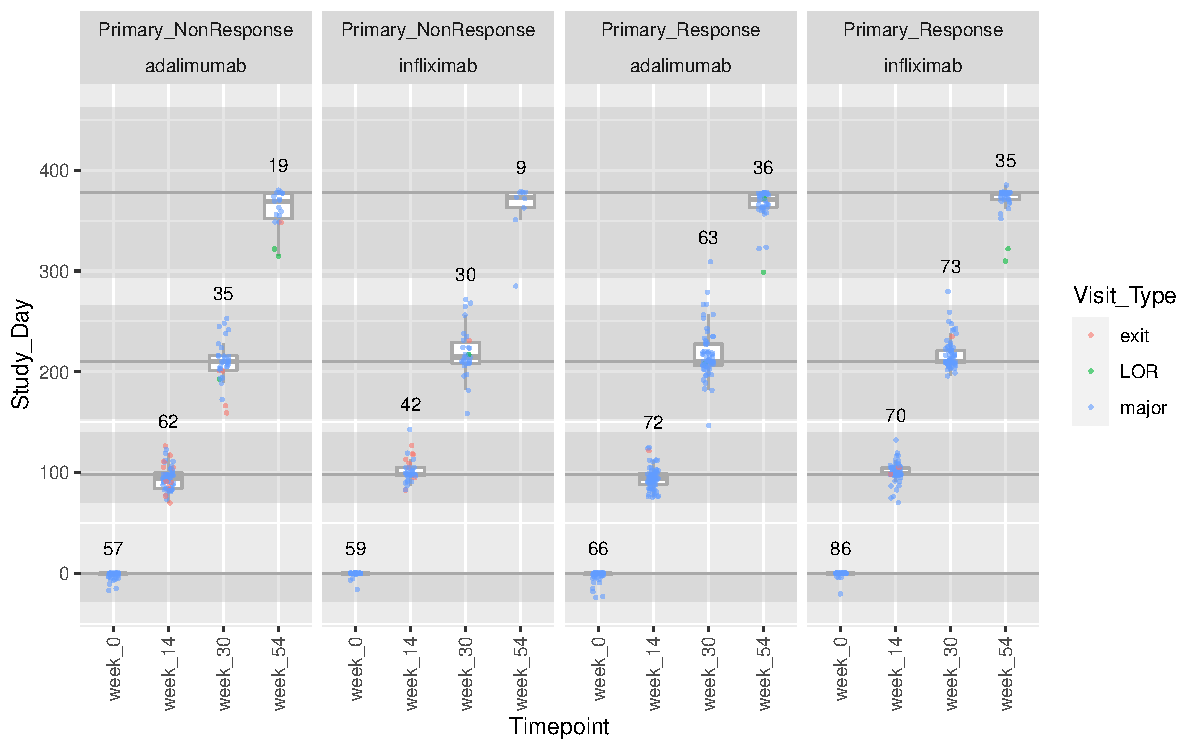
\includegraphics[width=1.0\textwidth,page=1]{mainmatter/figures/chapter_04/process_pheno.pheno_filtered_dge.Study_Day_vs_Visit_Label.pdf}
    \caption{
        \textbf{Number and sample day distribution for \gls{RNAseq} samples in each timepoint.}
        Windows for the four major visits are colored in grey. Samples mostly come from major visits, but a small number of \gls{LOR} and exit visit samples were included according to the criteria in \cref{subsubsec:multiPANTS_timepoints_def}.
    }
    \label{fig:multipants_studyDay_boxplots}
\end{figure}

\subsection{Definition of primary response and non-response}
\label{multiPANTS:PR_definition}

% "there is agreement that primary nonresponse to anti‐TNF drugs should not be assessed prior to 14 weeks following initial induction infusions with use of infliximab, or prior to 12 weeks for adalimumab injections" \autocite{dhaens2011LondonPositionStatement}
The definition of primary response and non-response was based on the clinical decision tree from \textcite{kennedy2019PredictorsAntiTNFTreatment}.
Primary response status was assessed at week 12, prior to the scheduled week 14 visit. 
The criteria for primary non-response was \emph{either} of the following: 
\begin{itemize}
    \item exit for treatment failure before week 14 (e.g. as decided by physician global assessment), \emph{or} corticosteroid use at week 14 (a continuing or new prescription);
    \item compared to week 0, a decrease in \gls{CRP} by less than 50\% or to >\SI{3}{\milli\gram\per\litre}, \emph{and} a decrease in \gls{HBI} by less than 3 points or to >4.
\end{itemize}
As \gls{PANTS} was an observational study that continued until drug withdrawal, a patient's clinician may have decided to continue anti-\gls{TNF} therapy even if a patient had primary non-response, so it was possible for non-responders to be sampled past week 14.
The criteria I used to define primary response\footnote{These are the criteria used by \textcite{kennedy2019PredictorsAntiTNFTreatment} to define week 14 remission.} was \emph{all} of the following:
\begin{itemize}
    \item not classified as a primary non-responder;
    \item \gls{CRP} \SI{\le 3}{\milli\gram\per\litre} by week 14;
    \item \gls{HBI} \SI{\le 4} by week 14.
\end{itemize}
Patients that only met a subset of criteria for either primary response or primary non-response were excluded.

% TODO: check this section. PNR is right, but PR is not  PNR is right, but PR is not "Response" on the flowchart, but "Remission"
% Selection criteria for samples from Nick:
%
% "~200 for each drug, ~100 PNR, 100 remission. PNR had to be PNR at week 14 and non-remission at week 54 (or unknown at week 54). 
% Remission had to have active disease at baseline and be in remission or response at week 14 and remission at week 54 (or unknown at week 54 and remission at week 30).
% ideal_downstream_cohort <- bd_vr_clin %>%
%   filter(
%     (crp_visit_1 >= 4 | calpro_visit_1 > 100),
%     (pnr & (is.na(remission_visit_5) | !remission_visit_5)) |
%     ((status_visit_2_3 %in% c("Response", "Remission")) & (remission_visit_5 | (is.na(remission_visit_5) & remission_visit_4)))
%   )
% They also had to be 16 years or over and have a baseline serum sample. 
% Within the infliximab patients, there was propensity matching between PNR/non-PNR based on on_imms_visit_1 + on_steroids_visit_1 + age_at_first_dose + earliest_weight_category_4 + albumin_visit_1 + sex."
There were additional inclusion criteria applicable to just the \gls{RNAseq} subcohort analyses in this chapter.
Patients were required to be at least 16 years old, and have an available baseline serum sample.
Primary non-responders were filtered to exclude patients in remission at week 54.

\subsection{Library preparation and \glsfmtshort{RNAseq}}

% From Mark:
% Here is an extended version of the protocol, with highlighting of the portion on poly-A selection and subsequent depletion steps:
%
% RNA and DNA were isolated from whole blood samples collected in Tempus Blood RNA Tubes.
%
% The Applied Biosystems Tempus Blood RNA Tube and Tempus Spin RNA Isolation kit was adapted to work in concert with the Qiagen QIAsymphony PAXgene Blood RNA (762635) and DNA DSP Midi (937255) Kit protocol for total RNA and DNA isolation from Tempus blood RNA tubes.
%
% Day 1: Batches of 48 tempus tubes were removed from -80°C and scanned into the electronic isolation record. Sample blood tube barcodes were matched to shipping barcodes and arranged by subject ID in visit order. Sample blood tubes were transferred to 4°C to thaw overnight. In preparation for DNA isolation, 48 14mL polystyrene culture tubes (BD352051) were labeled with Genomic Technologies barcodes and scanned into the electronic isolation record alongside the corresponding sample IDs.
%
% Day 2: Sample blood tubes were removed from 4°C and inverted 10 times to ensure efficient lysis. Samples were then left at room temperature to equilibrate for 2 hours. To obtain RNA and DNA from the same blood samples the following steps were performed: (1) Prepared the blood tube samples by following the Applied Biosystems manufacturer’s protocol “Processing Stabilized Blood before Purification” steps 1-5 (Nunc 50mL conical tubes 52000-004, PBS 1x -Ca2+ -Mg2+ pH 7.2 (20012050). After centrifugation, 2mL of the supernatant was aliquoted into the 14mL barcoded culture tubes for DNA isolation and placed in the 4°C until ready for the DNA isolation protocol with the Qiagen QIAsymphony DNA DSP Midi kit. The remaining supernatant was poured off of the RNA pellet and allowed to briefly dry. The blood samples then followed the Qiagen QIAsymphony PAXgene blood RNA manufacturer’s protocol at step 3. The following QIAsymphony instrument protocol was performed for isolation of Total RNA, RNA Isolation PAX RNA CR22332 ID 2915. The RNA samples were eluted in an 80uL volume and stored at -80°C, UltraPure DNase/RNase Free Distilled Water (10977023). The QIAsymphony was then loaded with the necessary reagents and consumables to perform the DNA isolation protocol. The DNA blood samples were removed from 4°C and loaded onto the QIAsymphony. The following QIAsymphony instrument protocol was performed for isolation of DNA, DNA isolation Blood_1000_V7-DSP. The DNA samples were eluted in a 200uL volume and stored at -80°C. RNA and DNA nucleic acid quantification were performed with the ThermoFisher QuBit BR RNA (Q10211) and QuBit BR dsDNA (Q32853) kits respectively, following the manufacturer’s protocol. RNA integrity analysis was performed with the Agilent RNA ScreenTape assay (5067-5579, 5067-5577, 5067-5576) on the Agilent 4200 TapeStation following the manufacturer’s protocol. Results were uploaded into the electronic isolation record and used RNA and DNA normalization.
%
% RNA library preparation from total RNA was conducted following the manufacturer’s protocol for the Kapa mRNA HyperPrep Kit. Briefly, 250 ng of total RNA was enriched for mRNA using magnetic oligo-dT beads. The remaining RNA was then fragmented by magnesium under elevated temperature. After fragmentation RNA was depleted of rRNA and globin mRNA using the QIAseq FastSelect RNA Removal Kit by Qiagen. The depleted RNA then underwent first strand synthesis using reverse transcriptase and random primers. Combined second strand synthesis and A-tailing incorporated dUTP into the second cDNA strand for stranded RNA sequencing and added dAMP to the 3’ ends for adapter ligation. The cDNA fragments were then ligated to sequencing adaptors (IDT xGEN Dual Index UMI adapters) and was enriched using 16 cycles of PCR. Final libraries were assessed using the Agilent Tapestation and Qubit (ThermoFisher) assay methods then sequenced on an Illumina HiSeq 4000 sequencer using 2x75bp read length.

Total RNA was extracted following the Qiagen QIAsymphony instrument protocol (RNA Isolation PAX RNA CR22332 ID 2915).
RNA was quantified with the ThermoFisher QuBit BR RNA (Q10211), 
and RNA integrity assessed with the Agilent RNA ScreenTape assay (5067-5579, 5067-5577, 5067-5576) on the Agilent 4200 TapeStation.

Library preparation was performed using the Kapa mRNA HyperPrep Kit, including enrichment for mRNA using magnetic oligo-dT beads, depletion of rRNA and globin mRNA using the QIAseq FastSelect RNA Removal Kit, and adapter ligation with IDT xGEN Dual Index UMI adapters.
Libraries were sequenced on the Illumina HiSeq 4000 with \si{75}{bp} paired-end reads.

\subsection{RNAseq quantification and preprocessing}

A total of 1141 samples from 396 patients were initially sequenced to a median depth of \textapprox{20} million read pairs.
Sequencing data was demultiplexed with Picard.
Total number of read pairs, sequence quality, overrepresented sequences, adapter content and sequence duplication rates were checked using FastQC.
% "To demultiplex and annotate the reads with the UMI information we use the Picard commands outlined in the attached file. We align using STAR (https://www.ncbi.nlm.nih.gov/pmc/articles/PMC3530905/ [ncbi.nlm.nih.gov]), mark and remove duplicates using UMITools (https://github.com/CGATOxford/UMI-tools [github.com]), and get our gene counts using featureCounts (http://subread.sourceforge.net/ [subread.sourceforge.net]). For QC we use fastQC, Picard, and compile the results together using MultiQC."
%
% "With the UMI protocol, raw fastq files are generated per sample/per lane, so there are 8 files per sample and they don’t actually contain the UMI information, so they are probably not ideal for starting your work. We should speak about where along the pipeline you are comfortable with us sending you the PANTS RNAseq
% Roughly the pipeline:
% Raw .bcl files -> demultiplexed unaligned .bam file per sample/per lane (8 files per sample) ->  fastq without UMI information per sample/per lane -> alignment -> aligned .bam files without UMI information per sample/per lane -> merge aligned .bam with unaligned .bam including UMI information -> merge .bam files for a sample across lane (1 file per sample) -> mark duplicates using UMIs -> create deduplicated .bam file -> create counts matrix and run QC -> optional creation of fastq files with UMIs in read names
Reads were mapped to GRCh38 using STAR (2.6.1d) and deduplicated to unique reads using UMI-tools.
Gene expression was quantified against the Ensembl 96 gene annotation with featureCounts (1.6.4).

Samples were filtered to remove outliers (\num{>2} standard deviations from the mean) according to percentage of aligned reads in coding regions reported by Picard, percentage of unique reads, and number of unique reads.
Samples that could not be mapped to a timepoint according to \cref{subsubsec:multiPANTS_timepoints_def} were removed.
Samples that came from patients with 
sex mismatch,
% based on Y chromosome gene expression,
grey zone primary response, 
or missing data for variables considered in the variable selection process (\cref{subsubsec:multiPANTS_var_selection}),
were removed.
A total of 814 samples remained after filtering.
The number of samples mapping to each timepoint as defined in \cref{subsubsec:multiPANTS_timepoints_def} is shown in \cref{fig:multipants_studyDay_boxplots}.
The number of samples per patient ranged from one to four, with a median of three (\cref{fig:multipants_visits_upset}).

\begin{figure}
    \centering
    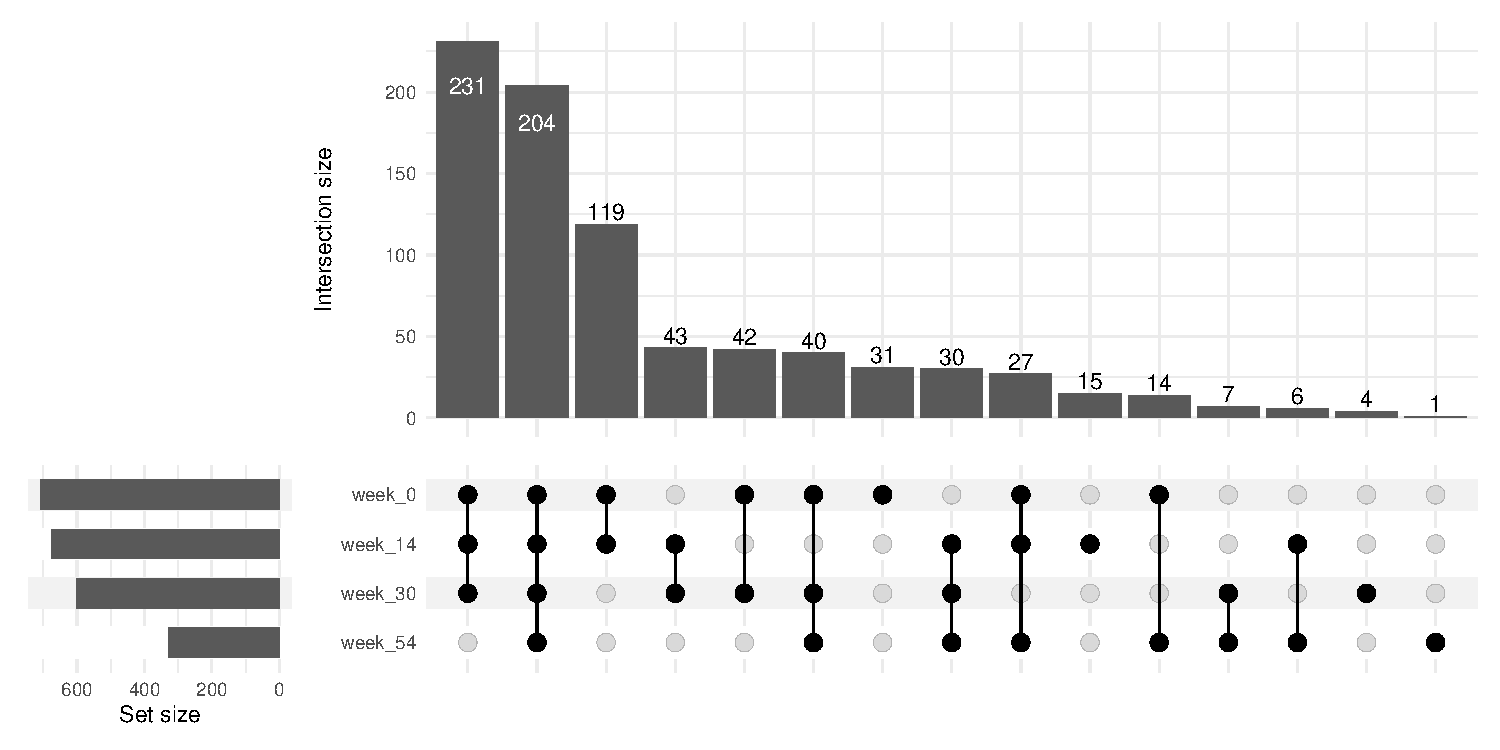
\includegraphics[width=1.0\textwidth,page=1]{mainmatter/figures/chapter_04/process_pheno.pheno_filtered_dge.Visit_Label_upset.pdf}
    \caption{
        \textbf{Distribution of \gls{RNAseq} samples from each patient among timepoints.}
    }
    \label{fig:multipants_visits_upset}
\end{figure}

The Ensembl 96 gene annotation contains \SI{58884} genes, many of which are not expressed in whole blood.
Effective library sizes were computed using the \gls{TMM} method in \software{edgeR} \autocite{robinson2010EdgeRBioconductorPackage}.
Between-sample normalisation for library size was performed using \software{edgeR::cpm}, converting counts to \gls{CPM}.
Genes with low expression were filtered,
requiring >1.25 CPM in >10\% of samples (1.25 \gls{CPM} was approximately 10 counts at the median library size of 8 million unique mapped read pairs),
and non-zero expression in >90\% of samples.
% NOTE: probably don't need to remove these manually in future.
Globin genes and short \glspl{ncRNA} were removed.
A total of \num{15511} genes remained after filtering.
Finally, \glspl{CPM} were converted to the $\log_{2}$ scale, and precision weights to account for the expression mean-variance relationship were computed for each gene and sample using \software{voomWithDreamWeights} from \software{variancePartition} \autocite{hoffman2016VariancePartitionInterpretingDrivers}.

\subsection{\Glsfmtlong{DGE}}

\subsubsection{Variable selection by variance components analysis}
\label{subsubsec:multiPANTS_var_selection}

% TODO: arrows are directed causal effects, so remove these if talking about association
For each gene, the \gls{DGE} model was a regression expressing the response variable, gene expression, 
as a linear function of predictor variables of interest (primary response status, drug, timepoint),
and other selected predictor variables.
In estimating the association of predictor X to response Y by regression, 
adjustment for a third variable Z can increase, decrease, or even reverse the effect estimate of X (the regression coefficient).
I aimed to select third variables for inclusion into the \gls{DGE} model that were covariates,
defined here as a Z that is associated with Y, but not with X.
Such variables are also known as neutral controls \autocite{cinelli2020CrashCourseGood}, precision variables, or prognostic variables,
At the cost of 1 \gls{df},
Z explains variation in Y that would otherwise be considered residual,
so conditioning on Z increases the efficiency of estimating the effect of X on Y, but does not change the effect estimate.

Many variables were available for selection;
\cref{fig:multipants_pheno_filtered_ggcorrplot} shows their correlation matrix.
% Univariable analyses showed the strongest associations with primary non-response to infliximab and adalimumab were with week 14 drug and anti-drug antibody concentrations (table 3; appendix p 17).
% Primary non-response to infliximab was also associated with older age at first dose, smoking at baseline, non-use of an immunomodulator at baseline, lower baseline albumin concentrations, and higher baseline white cell count.
% Primary non-response to adalimumab was associated with a higher body-mass index at baseline.
These included three variables associated with primary response in \textcite{kennedy2019PredictorsAntiTNFTreatment}: baseline immunomodulator use, smoking and \gls{BMI}.
% From Mark:
% As a follow-up, here is what Sam shared about estimating cell composition in the data: “We used the Houseman method [bmcbioinformatics.biomedcentral.com], which is implemented with the estimateCellCounts() function from the minfi package in R.”
Also available were proportions of six common cell types in whole blood 
(CD4\textsuperscript{+} T cells, CD8\textsuperscript{+} T cells, B cells, \gls{NK} cells, monocytes, granulocytes),
estimated using the Houseman method (\software{minfi::estimateCellCounts} \autocite{aryee2014MinfiFlexibleComprehensive})
from whole blood Illumina MethylationEPIC methylation array data collected from the same patients and timepoints.
The Houseman method uses differentially methylated regions between immune cell types as cell type markers \autocite{houseman2012DNAMethylationArrays}.

% TODO: labels here don't match listings
\begin{figure}
    \centering
    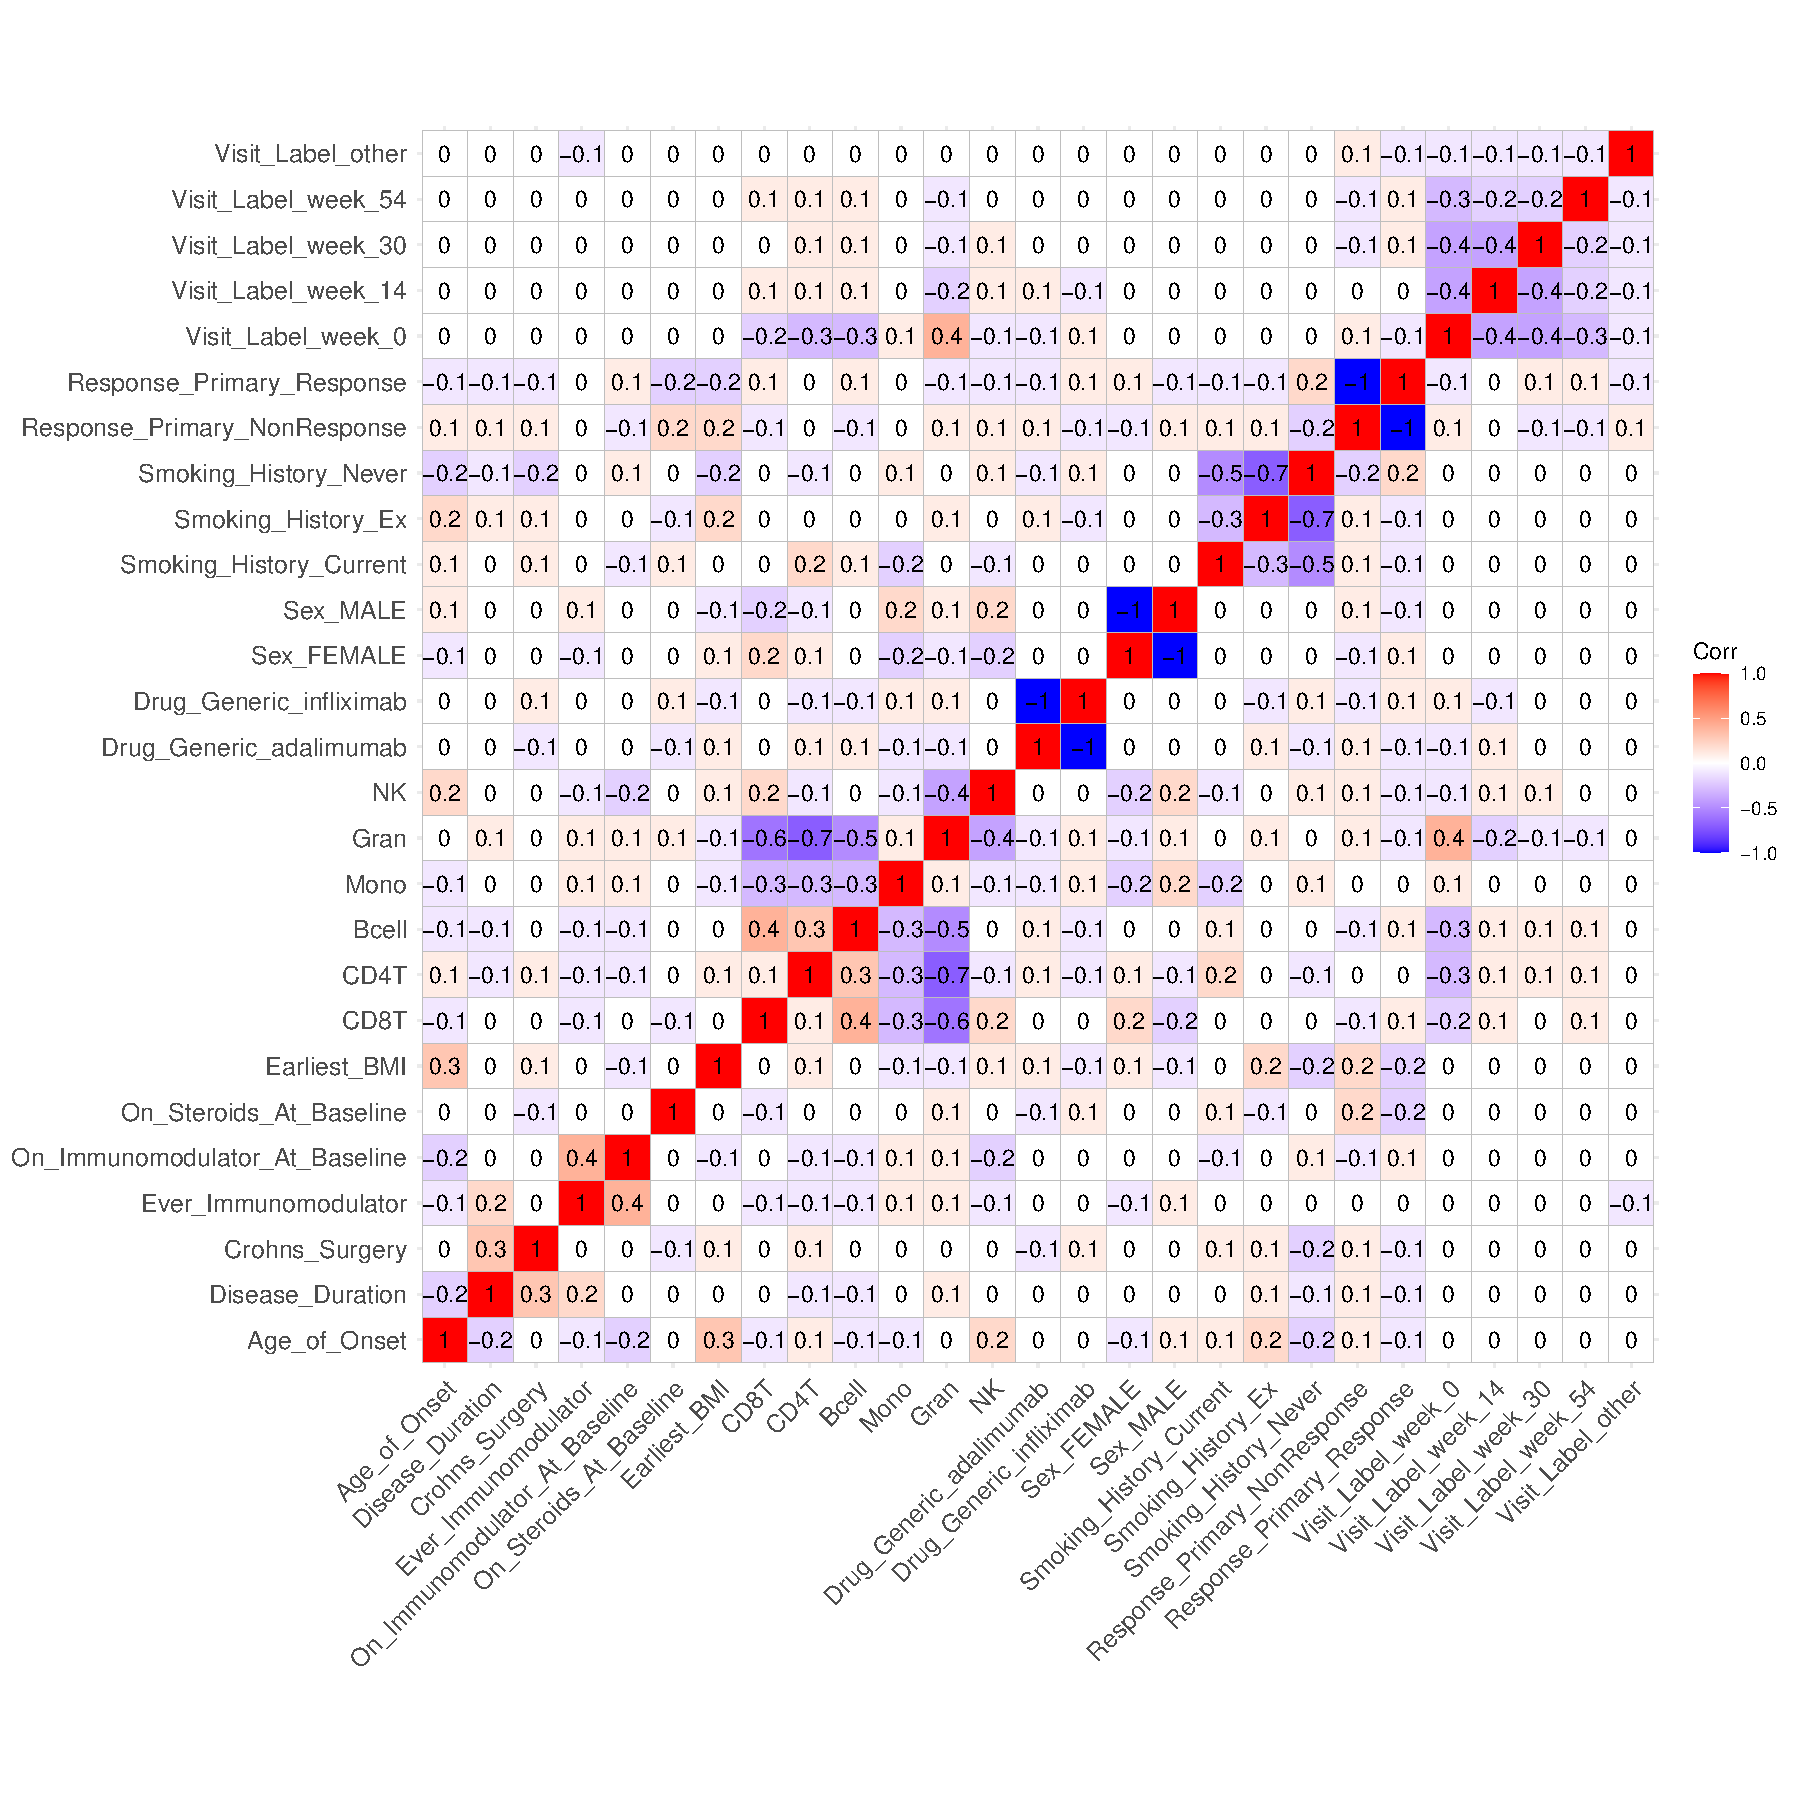
\includegraphics[width=1.0\textwidth,page=1]{mainmatter/figures/chapter_04/process_pheno.pheno_filtered_dge.ggcorrplot.pdf}
    \caption{
        \textbf{Correlation matrix of variables measured in \gls{PANTS} that were considered as potential independent variables.}
        NK = \gls{NK} cell, Gran = granulocyte, Mono = monocyte, Bcell = B cell, CD4T = CD4+ T cell, CD8 = CD8+ T cell.
    }
    \label{fig:multipants_pheno_filtered_ggcorrplot}
\end{figure}

% \1 Visualised main factors that influence global gene expression by PCA (\cref{fig:multipants_dream_prcomp})
%     \2 main separation along PC1 is w0 anti-TNF naive samples from all other post-drug start samples

% \begin{figure}
%     \centering
%     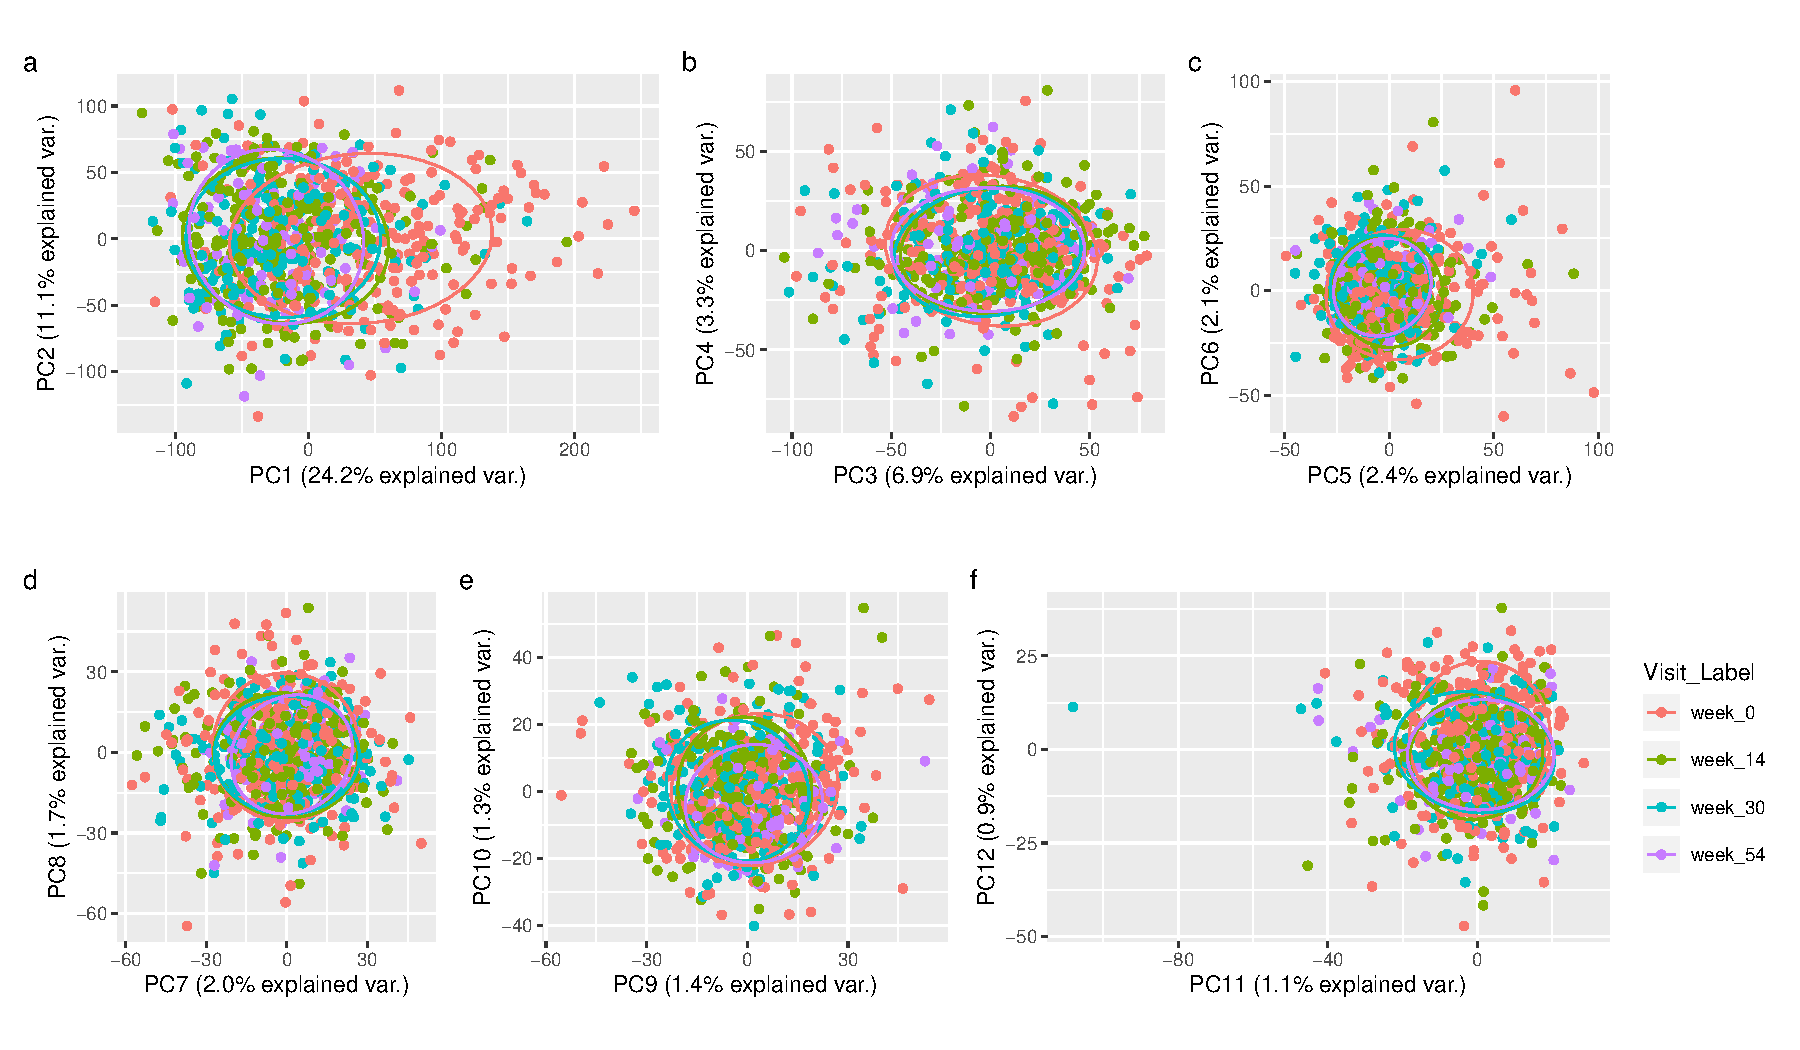
\includegraphics[width=1.0\textwidth,page=1]{mainmatter/figures/chapter_04/dream.prcomp.pdf}
%     \caption{top 12 expression PCs of filtered expression data}
%     \label{fig:multipants_dream_prcomp}
% \end{figure}

A variance components analysis was performed to quantify the proportion of expression variance explained by each variable for each gene using \software{variancePartition} \autocite{hoffman2016VariancePartitionInterpretingDrivers}.
Variables that do not explain much variation in the response are unlikely to improve efficiency if conditioned on.
The model was a mixed effects regression model with variables in \cref{fig:multipants_pheno_filtered_ggcorrplot} included as predictors.
Additional categorical variables were included for patient and \gls{RNAseq} library preparation plate.
An additional continuous variable consisting of random numbers drawn from the standard normal distribution was also included as a null.
% The var explained by Gran will be redistributed among highly cor vars anyways.
Granulocyte proportion estimates were dropped to relieve perfect multicollinearity.
Categorical variables were coded as random intecepts, and continuous variables as fixed effects.
Surprisingly, simulations from \textcite{hoffman2016VariancePartitionInterpretingDrivers} showed variance proportion estimates were unbiased even when coding categorical variables with as few as two categories as random effects. 
This was the case as long as model parameters were estimated using \gls{ML} rather than \gls{REML}. 
% which is commonly used for variance components analysis.
It was also shown this approach avoids overestimates of variance proportions that occur if categorical variables with many levels are treated as fixed.

As downstream \gls{DGE} methods require the same set of predictors for all genes, the aim was to select variables that explain a lot of variance for many genes.
Variables that explained the most variance on average were patient, cell proportions and \gls{RNAseq} plate (\cref{fig:multipants_varPart}).
Some variables that did not explain more variance on average than the null nevertheless had high maximum values, indicating their importance for a relatively small number of genes.
These included sex, library preparation protocol version, and smoking status.
However primary response status---a variable of interest---also fell into this group,
so it was difficult to justify excluding all variables with lower median variance explained than the null.
Consequently, all non-null variables in \cref{fig:multipants_varPart} were selected as predictors in downstream models apart from \enquote{Ever\_Immunomodulator} 
(whether the patient had ever had immunomodulator treatment), 
as that variable had both low median variance explained and was correlated with baseline immunomodulator use.
This is a crude approach, but the sample size is large compared to number of \glspl{df} lost by including predictors that may not be relevant for some genes.
% TODO: check robustness of DGE results to predictor set

\begin{figure}
    \centering
    \includegraphics[width=1.0\textwidth,page=1]{mainmatter/figures/chapter_04/dream.plotVarPart.pdf}
    \caption{
        \textbf{Variance components analysis showing distribution of per-gene percentage of variance in expression explained by each variable.}
        Variables are ordered by the median of per-gene variance proportion estimates.
        random\_numbers is the null, drawn from the standard normal distribution.
        PANTS.ID = patient ID, NK = \gls{NK} cell, Gran = granulocyte, Mono = monocyte, Bcell = B cell, CD4T = CD4+ T cell, CD8 = CD8+ T cell.
}
    \label{fig:multipants_varPart}
\end{figure}

How might interpretations of effect sizes of interest be affected by including this suite of other variables, all of which can be considered as third variables?
If a third variable Z is not a precision variable, but is also associated with X, conditioning changes the effect estimate.
The regression model is mathematically agnostic to causal relationships between variables,
but distinct types of third variable can be distinguished conceptually by assuming the direction of causal relationships \autocite{mackinnon2000EquivalenceMediationConfounding}.
Conditioning on a confounder ($X \leftarrow Z \rightarrow Y$) reduces bias of the effect estimate,
conditioning on a collider ($X \rightarrow Z \leftarrow Y$) induces bias,
and conditioning on a mediator in the causal path ($X \rightarrow Z \rightarrow Y$) changes the effect estimated by removing the indirect effect mediated by Z,
usually biasing the effect estimate towards zero\footnote{It is not easy to determine the direction of bias (positive or negative) for any of these cases in general \autocite{suzuki2020CausalDiagramsPitfalls}.}.

From the variance partition analysis (\cref{fig:multipants_varPart}), cell proportions were among the biological factors that explained the most variance on average,
they are one of the largest sources of variation in bulk blood expression data, 
and are a major driver of immune response to perturbations \autocite{piasecka2018DistinctiveRolesAge}.
% They change a lot over time too (\cref{fig:multipants_cell_type_proportion_vs_Study_Day})
Thus I decided to I fit two sets of separate \gls{DGE} models including and excluding cell proportions as predictors, but otherwise identical.
Assuming that cell proportions act as a mediator of the drug's effect on gene expression, these models have complementary interpretations.
In models without cell proportions included, differential expression after drug perturbation could represent up or downregulation on a per cell basis, 
but could also come from differences in cell proportions induced by the drug.
The estimates from models adjusted for cell proportions are more likely to reflect up or downregulation on a per cell basis.
% \todo{Could cell proportions act as colliders?}
When comparing expression between responders and non-responders,
one might also assume cell proportions can mediate the effect of a patient's response status on expression%
\footnote{
    The assumption that response status is a stable property of a patient that can be treated as an independent variable will be discussed in \cref{sec:discussion_responderAnalysis}.
}.
Analogously, estimates of expression differences between responders and non-responders from the two sets of models 
also have complementary interpretations: total difference, and per-cell differences not due to differences in cell proportions.
Throughout this chapter, I interpret the estimates from both sets of models accordingly.

% \begin{figure}
%     \centering
%     \includegraphics[width=1.0\textwidth,page=1]{mainmatter/figures/chapter_04/dream.cell_type_proportion_vs_Study_Day.pdf}
%     \caption{changes in cell proportions of 6 immune cell types over time}
%     \label{fig:multipants_cell_type_proportion_vs_Study_Day}
% \end{figure}

\subsubsection{Contrasts for pairwise group comparisons}

Per-gene \gls{DGE} models were fit in \software{dream} \autocite{hoffman2020DreamPowerfulDifferential}.
Like the variance partition model models, these \gls{DGE} models were linear mixed models:
%
% \begin{lstlisting}
% Expression ~
%     0 +
%     concat(Visit, Response, Drug) +
%     Sex + Age_of_Onset + Disease_Duration +
%     Smoking_History + Crohns_Surgery +
%     On_Immunomodulator_At_Baseline +
%     On_Steroids_At_Baseline + Earliest_BMI +
%     [CD8T + CD4T + Bcell + Mono + NK] +
%     Library_Prep_Protocol +
%     (1 | RNA_Plate) +
%     (1 | Patient)
% \end{lstlisting}
%
\begin{equation}
y = 0 + \beta_{trd} G_{trd} + \sum_{}^{9}{\beta_Z Z} + (\sum_{}^{5}{\beta_C C}) + u + v + \epsilon
\label{eq:multiPANTS_dge_model}
\end{equation}
where:
\begin{itemize}
    \item the response variable is gene expression $y$.
    \item 0 indicates there is no intercept term.
    \item $G_{trd}$ is a fixed effect for experimental group defined by combinations of the predictors of interest:
        timepoint (week 0, 14, 30, 54), 
        response (responder, non-responder), 
        and drug (infliximab, adalimumab).
        This is equivalent to having an intercept term and a three-way interaction between visit, response, and drug, including all lower order terms,
        but is more convenient for testing pairwise expression differences between groups,
        as the coefficient for each term is the estimate of mean expression for that group.
        % TODO: move variable descriptions up
    \item $\sum_{}^{9}{\beta_Z Z}$ are the non-cell proportion fixed effects chosen in \cref{subsubsec:multiPANTS_var_selection}:
        sex (Sex), 
        age of disease onset (Age\_of\_Onset), disease duration (Disease\_Duration), 
        smoking history (Smoking\_History: ex, current or never), 
        whether the patient has had surgery for \gls{CD} (Crohns\_Surgery), 
        whether the patient was on immunomodulator at baseline (On\_Immunomodulator\_At\_Baseline), 
        whether the patient was on steroids at baseline (On\_Steroids\_At\_Baseline), 
        \gls{BMI} at baseline (Earliest\_BMI),
        and library preparation protocol version (Library\_Prep\_Protocol).
    \item $\sum_{}^{5}{\beta_C C}$ are the cell proportion fixed effects chosen in \cref{subsubsec:multiPANTS_var_selection},
        for \gls{NK} cells, monocytes, B cells, CD4+ T cells, and CD8+ T cells.
    \item $u$ is a random intercept for \gls{RNAseq} plate (RNA\_Plate).
    \item $v$ is a random intercept for patient (PANTS.ID), nested inside \gls{RNAseq} plate.
\end{itemize}

As the interest was in estimating a single coefficient for each predictor's effect size on expression (rather than estimating variance components), 
most predictors above are modelled as fixed effects.
Since \gls{RNAseq} plate and patient are nuisance variables with a large number of levels they are modelled as random intercepts.
A total of four sets of per-gene models were fit,
with and without the cell proportion terms $\sum_{}^{5}{\beta_C C}$,
and replacing $\beta_{trd} G_{trd}$ (separate drug models) with $\beta_{tr} G_{tr} + \beta_d d$ (pooled drug models) or not.
% https://web.stanford.edu/class/psych252/section/Mixed_models_tutorial.html#reml-vs.ml
% You should use ML when comparing models that differ in their fixed effects
% [...]
% In REML (REstricted ML) estimation, our main interest is in estimating the random effects, not the fixed effects.
% Imagine that we restrict our parameter space by setting the fixed effects parameters in set (i) above to certain plausible values.
% [...]
% it should not be used to compare models that differ in their fixed effects structure. You should just use this when comparing models that differ in their random effects.
%
% \gls{REML} treats fixed effects as nuisance parameters and estimates random effects after first integrating out fixed effects \autocite{mcneish2017SmallSampleMethods}.
As we are no longer performing variance components analysis,
to avoid small-sample bias in estimates of fixed effect standard errors, \gls{REML} was used for estimation \autocite{mcneish2017SmallSampleMethods}.

Specific hypotheses were tested using sum-to-zero contrasts, which are linear combinations of the model coefficients with weights summing to zero.
For example, 
to test for \gls{DGE} between responders and non-responders to infliximab at baseline in the non-pooled model,
I used a contrast where
the weight for the (week 0, responder, infliximab) group coefficient was 1,
the weight for the (week 0, non-responder, infliximab) group coefficient was -1,
and all other coefficient weights were 0.
% Contrasts can be used thuswise to compare any pair of groups, as the coefficients of group terms are group means.
%
% However, in the lme4 package in R the standards for evaluating significance of
% fixed effects in these models (i.e., obtaining p-values) are somewhat vague.
% There are good reasons for this, but as researchers who are using these models
% are required in many cases to report p-values, some method for evaluating the
% significance of the model output is needed.
%
% The primary motivation for this omission is that in linear mixed models it is
% not at all obvious what the appropriate denominator degrees of freedom to use
% are, except perhaps for some simple designs and nicely balanced data.
% 
% \2 to get p values for papers, Dream uses lmerTest approximation Satterthwaite df with REML
% \2 this combo controls type 1 error for n>144 in lmerTest simulations \url{https://link.springer.com/article/10.3758/s13428-016-0809-y}
To get \pvalues{}, the contrast divided by its standard error was compared to the $t$-distribution using the Satterthwaite approximation for \glspl{df}.
% \2 FDR BH separately per comparison: "The default method="separate" and
% adjust.method="BH" settings are appropriate for most analyses.
% method="global" is useful when it is important that the same t-statistic
% cutoff should correspond to statistical significance for all the
% contrasts." \url{https://rdrr.io/bioc/limma/man/decideTests.html}
\Gls{FDR} was controlled with the \gls{BH} method, threshold set at 0.05, computed separately for each contrast\footnote{
It could also have been computed globally over all contrasts if it were necessary to have the same $t$-statistic threshold for statistical significance in all contrasts.
}.

% NOTE: to get confidence intervals for FDR https://bmcbioinformatics.biomedcentral.com/articles/10.1186/1471-2105-12-288
% https://en.wikipedia.org/wiki/False_coverage_rate

\subsubsection{Spline model of expression over time}

% NOTE: there are tailored methods for time series DGE, but I did not use them due to shortness of this time series
% "Comparative analysis of differential gene expression tools for RNA sequencing time course data"
% Surprisingly, TC tools were outperformed by the classical pairwise comparison approach on short time series (<8 time points) in terms of overall performance and robustness to noise, mostly because of high number of false positives, with the exception of ImpulseDE2.
% Also see:
% Clustering time-course Microarray data using functional Bayesian infinite mixture model
% clustering folder in downloads
% https://2-bitbio.com/2017/04/clustering-rnaseq-data-making-heatmaps.html
% https://hbctraining.github.io/DGE_workshop/lessons/08_DGE_LRT.html

The aim was to use expression data from all four timepoints to find genes associated with response,
while avoiding a large number of pairwise comparisons.
I fit a natural cubic spline (\software{splines::ns}) to the study day to allow for non-linear trajectories of expression over time.
A cubic spline is a continuous function defined piecewise in each successive interval between a set of $k$ knots in the range of the input variable.
The $k-1$ pieces between knots are polynomials of degree 3. 
For a natural spline, the function is constrained to be linear outside of the boundary (first and last) knots to avoid unpredictable behaviour at the boundaries \autocite{perperoglou2019ReviewSplineFunction}.
%
% \begin{lstlisting}
% Expression ~
%      1 +
%      Primary_Response * ns(Study_Day, knots=7*c(14, 30)) +
%      Drug_Generic +
%      Sex + Age_of_Onset + Disease_Duration +
%      Smoking_History + Crohns_Surgery +
%      On_Immunomodulator_At_Baseline +
%      On_Steroids_At_Baseline + Earliest_BMI +
%      [CD8T + CD4T + Bcell + Mono + NK] +
%      Library_Prep_Protocol +
%      (1 | RNA_Plate) +
%      (1 | PANTS.ID)
% \end{lstlisting}
%
I set two inner knots at week 14 and week 30, as expression is expected to change after each drug dose.
To include all data to within the boundaries, the two boundary knots were set at the minimum and maximum values of study day rather than week 0 and week 54.
% "Function ns() from package splines indeed implements a natural cubic spline (aka restricted cubic spline) but using a B-splines basis representation. This provides an equivalent fit but it is not the same as the expansion you wrote in math. This expansion is implemented in function rcs() from the package rms."
% The function ns(Study\_Day, knots=7*c(14, 30)) returns a basis matrix for the spline with 3 \gls{df} (3 columns).
A basis matrix \autocite{perperoglou2019ReviewSplineFunction} was computed with \software{ns(Study\_Day, knots=7*c(14, 30))},
which is a matrix with 3 columns, each column being a transformation of the input, study day.
The columns are fit in the regression model in place of study day to allow for non-linear effects of study day on expression.
The model form used was as in \cref{eq:multiPANTS_dge_model},
except with $\beta_{trd} G_{trd}$
replaced by $\beta_r r + \sum_{}^{3}{\beta_b b} + \sum_{}^{3}{\beta_{rb} rb} + \beta_d d$,
where $r$ is response status,
$\sum_{}^{3}{\beta_b b}$ are the three columns of the basis matrix,
and $\sum_{}^{3}{\beta_{rb} rb}$ are the second-order interaction terms between response status and the basis matrix columns.
Separate sets of per-gene models were again fit with and without cell proportions $\sum_{}^{5}{\beta_C C}$.

% NOTE: true for poly, not true for ns
% https://stackoverflow.com/questions/19484053/what-does-the-r-function-poly-really-do
% Unfortunately there is an undesirable aspect with ordinary polynomials in regression. If we fit a quadratic, say, and then a cubic the lower order coefficients of the cubic are all different than for the quadratic [...]
% What we would really like is to add the cubic term in such a way that the lower order coefficients that were fit using the quadratic stay the same after refitting with a cubic fit. To do this take linear combinations of the columns of poly(horsepower, 2, raw = TRUE) and do the same with poly(horsepower, 3, raw = TRUE) such that the columns in the quadratic fit are orthogonal to each other and similarly for the cubic fit. That is sufficient to guarantee that the lower order coefficients won't change when we add higher order coefficients.
% [...]
% Importantly, since the columns of poly(horsepwer, 2) are just linear combinations of the columnns of poly(horsepower, 2, raw = TRUE) the two quadratic models (orthogonal and raw) represent the same models (i.e. they give the same predictions) and only differ in parameterization.
%
% http://www.science.smith.edu/~jcrouser/SDS293/labs/lab12-r.html
% This syntax fits a linear model, using the lm() function, in order to predict wage using a fourth-degree polynomial in age: poly(age,4). The poly() command allows us to avoid having to write out a long formula with powers of age. The function returns a matrix whose columns are a basis of orthogonal polynomials, which essentially means that each column is a linear combination of the variables age, age^2, age^3 and age^4.
% If we prefer, we can also use poly() to obtain age, age^2, age^3 and age^4 directly. We can do this by using the raw = TRUE argument to the poly() function. Later we see that this does not affect the model in a meaningful way -- though the choice of basis clearly affects the coefficient estimates, it does not affect the fitted values obtained.

To test for response-associated differences in the spline parameters, 
the predictors of interest are the interaction terms $\sum_{}^{3}{\beta_{rb} rb}$. 
% TODO F-test to p value
% f-test, is basically a wald test
% https://support.bioconductor.org/p/6124/
% The above mentioned statistics are computed for every contrast for each gene.
% The eBayes() function computes one more useful statistic. The
% moderated F-statistic (F) combines the t-statistics for all the
% contrasts for each gene into an overall test of significance for that
% gene. The moderated F-statistic tests whether any of the contrasts
% are non-zero for that gene, i.e., whether that gene is differentially
% expressed on any contrast. The moderated-F has numerator degrees of
% freedom equal to the number of contrasts and denominator degrees of
% freedom the same as the moderated-t. Its p-value is stored as
% fit$F.p.value. It is similar to the ordinary F-statistic from
% analysis of variance except that the denominator mean squares are
% moderated across genes.
The three terms are tested jointly with an F-test, and \gls{FDR} correction was performed with the \gls{BH} method, with the threshold set at 0.05.
A significant result indicates a significant difference in the trajectory of expression over study day between responders and non-responders, which may be non-linear.

\subsubsection{Clustering expression over all timepoints}

I clustered genes by their expression trajectories,
to define sets of genes with similar trajectories over time for input into gene set enrichment analyses.
This was done to aid interpretation of significant genes from the cell proportion adjusted spline model.
Expression data was converted to the \gls{CPM} scale using \gls{TMM} normalisation factors, then regressed against cell proportions.
Residuals were centered and scaled per gene, 
A distance matrix was computed using 1 - Pearson correlation as the distance metric.
% which is scale invariant on centered data https://www.researchgate.net/publication/26290974_A_new_approach_for_clustering_gene_expression_time_series_data
Hierarchical clustering was performed with complete agglomeration for inter-cluster distance (fastcluster::hclust(method='complete')).
The optimal number of clusters was determined using the gap statistic (\software{factoextra::fviz\_nbclust(method='gap\_stat', nboot=500)}),
which determines when the change in within-cluster dispersions are no longer significantly improved by increasing the number of clusters \autocite{tibshirani2001EstimatingNumberClusters}.
The hierarchical clustering tree was then cut into that number of clusters.

% Other possible approaches with more direct connection to spline model fit?
% e.g. clustering basis function results
% e.g. predicted values of expression

% How to account for levels of noise in expression data?
% TMixClust
% measurements come withintrinsic noise which makes their time series clustering a difficult task. Here, we show howto cluster such data with the package TMixClust. TMixClust is a soft-clustering methodwhich employs mixed-effects models with nonparametric smoothing spline fitting and is ableto robustly stratify genes by their complex time series patterns.
% \url{https://www.nature.com/articles/s41598-018-36135-3}

\subsubsection{Gene set enrichment analyses}

Rank-based gene set enrichment analyses were conducted using \software{tmod::tmodCERNOtest} \autocite{weiner3rd2016TmodPackageGeneral} and \glspl{BTM}, as described in \cref{subsec:hird_dge_geneSetEnrichment}.
%
% TODO: clarify how the transformations work in dream
% https://www.bioconductor.org/packages/devel/bioc/vignettes/variancePartition/inst/doc/dream.html
% Since dream uses an estimated degrees of freedom value for each hypothsis test, the degrees of freedom is different for each gene here. Therefore, the t-statistics are not directly comparable since they have different degrees of freedom. In order to be able to compare test statistics, we report z.std which is the p-value transformed into a signed z-score. This can be used for downstream analysis.
% [...]
% Since dream uses an estimated degrees of freedom value for each hypothsis test, the degrees of freedom is different for each gene here. Therefore, the F-statistics are not directly comparable since they have different degrees of freedom. In order to be able to compare test statistics, we report F.std which is the p-value transformed into an F-statistic with df1=number of coefficiets tested and df2=Inf. This can be used for downstream analysis.
For each contrast, 
as the $t$-statistics are not comparable between genes due to the use of approximate \glspl{df},
I ranked genes by the signed Z score reported by \software{dream}, which is a monotonic transformation of the \pvalue{}.
Similarly, moderated F-statistics from the spline are not comparable between genes, so I used the signed F-statistic reported by \software{dream} from the transformation of the \pvalue{}.

Gene set overrepresentation analyses with the hypergeometric test were conducted with \software{tmod::tmodHGtest} as detailed in \cref{subsec:hird_reQTL_geneSetEnrichment}.

% TODO: add explanation of interaction term column
% Note that we can rank by main effect or interaction Z score.
% For interactions, interpretation depends on the original signs of effects.

\subsection{Genotyping and genotype data preprocessing}

% sazonovs2019HLADQA105Carriage
% DNA was extracted from pretreatment blood samples from
% 1524 patients in the PANTS cohort and genotyping undertaken
% using the Illumina CoreExome microarray
%
% After quality
% control, 1323 patients remained in the study, of which
% 1240 had drug and anti-drug antibody level data available
% (Supplementary Figure 2).
%
% 7,578,947 variants with an information content metric score .4 were subsequently taken forward for analysis
%
% HLA types were imputed at 2- and 4-digit resolution for the
% following loci: HLA-A, HLA-C, HLA-B, HLA-DRB1, HLA-DQA1,
% HLA-DQB1, and HLA-DPB1.
%
% sex,
% drug type (infliximab or adalimumab), immunomodulator use,
% and the first within-sample principal component were
% included as covariates (Supplementary Table 2).
%
% NOTE: QC details here also from Alex's thesis
Genotype data were subsetted from the post-quality control \gls{PANTS} cohort genotypes used in \textcite{sazonovs2019HLADQA105Carriage},
where the preprocessing pipeline is described in full detail.
These data are from whole blood samples collected into EDTA tubes at week 0 and genotyped on the Illumina CoreExome genotyping array.
Pre-imputation quality control was performed as described in \textcite{delange2017GenomewideAssociationStudy}.
Imputation was performed using the Sanger Imputation Service with the Haplotype Reference Consortium panel.
Post-imputation, samples that were non-European, related (proportion identity-by-descent > 0.1875), or were outliers in genotype missingness or heterozygosity rate were removed;
\glspl{SNP} that were poorly imputed (INFO score < 0.4), deviated from \gls{HWE} (p < 1e-10), had high missingness (> 5\%), or low \gls{MAF} (< 1\% before subsetting) were removed.
\num{7503762} \glspl{SNP} remained after filtering.
Genotypes were converted to dosages of the non-reference allele.

\subsection{\Glsfmtlong{reQTL} mapping}

The overall strategy and methods used were largely identical those those used in \cref{ch:hird_reQTL}, laid out in \cref{sec:hird_reQTL_methods}.
Differences are described below.

\subsubsection{Computing genotype PCs}

Samples were projected onto \glspl{PC} defined by 1000 Genomes Project samples using \gls{SNP} weights from {akt}\footnote{\url{https://github.com/Illumina/akt}},
confirming that samples were of European ancestry (\cref{fig:multipants_genotype_akt_1000g_pca}).
% The first four \glspl{PC} in the HapMap 3 were found to be significant according to the Tracy-Widom test in \cref{subsec:hird_dge_genotype_pc}.
% This implies that EIGENSTRAT results are not sensitive to the number of axes of variation used, as long as there is a sufficient number of axes to capture true population structure effects.
% We see that in each SNP category, results are virtually identical for K = 1, 2, 5 or 10.
Here I chose the first five \glspl{PC} for use downstream, one more than was chosen in \cref{subsec:hird_dge_genotype_pc} by Tracy-Widom test.
This should be sufficient, as the \gls{PANTS} cohort is less ethnically diverse than the \gls{HIRD} cohort.
% the specific number is not important, as long as a sufficient number of \glspl{PC} are included to capture large-scale population structure \autocite{price2006PrincipalComponentsAnalysis}.
\glspl{PC} were centered and scaled before downstream use to improve model convergence.

\begin{figure}
    \centering
    \includegraphics[width=1.0\textwidth,page=1]{mainmatter/figures/chapter_04/pants_samples.sampleids_cleaned_to_lowercase.filtered.GRCh38.sorted.multiPANTS.projection_1000G_pca.pdf}
    \caption{
        \textbf{1000G samples and PANTS samples projected onto 1000G genotype PC1 and PC2 axes, colored by superpopulation (a) and population (b).}
        1000G superpopulations: AFR = African, AMR = Ad Mixed American, EAS = East Asian, EUR = European, SAS = South Asian.
        1000G European populations: CEU = Utah Residents (CEPH) with Northern and Western European Ancestry, FIN = Finnish in Finland, GBR = British in England and Scotland, IBS = Iberian Population in Spain, TSI = Toscani in Italia.
    }
    \label{fig:multipants_genotype_akt_1000g_pca}
\end{figure}

\subsubsection{Finding hidden confounders in expression data}

Between-sample normalisation and variance stabilisation was applied to the counts matrix (DESeq2::vst), resulting in $\log_2$ scale expression estimates.
As described in \cref{sec:hird_reQTL_methods},
given known factors (response, drug, five scaled genotype \glspl{PC}, five cell proportions), 
{PEER} was used to find additional hidden factors that explain variance in the expression matrix for a large fraction of genes.
This is similar to the process undertaken in \cref{subsubsec:multiPANTS_var_selection}, but these hidden factors can be unmeasured.
To maximise efficiency for \textit{cis}-\gls{eQTL} mapping, 
the number of PEER factors retained for each timepoint was selected to maximise the number of genes with at least one significant \gls{eQTL} detected on chromosome 1 (\cref{fig:multipants_reqtl_PEER_k_choice}).
The selected numbers were 25, 20, 15, and 5 factors for weeks 0, 14, 30, and 54 respectively.

\begin{figure}
    \centering
    \includegraphics[width=1.0\textwidth,page=1]{mainmatter/figures/chapter_04/count_eGenes.signif_eGenes_vs_PEER_n.dataset_multiPANTS.chr_1.pdf}
    \caption{
        \textbf{Number of eGenes significant on chr1 vs. number of PEER factors included in \gls{eQTL} mapping as covariates.}
        \gls{FDR} computed with hierarchical Bonferroni-\gls{BH} \autocite{huang2018PowerFalseDiscovery} with significance threshold set at 0.05.
    }
    \label{fig:multipants_reqtl_PEER_k_choice}
\end{figure}

\subsubsection{Computing kinship matrices}

% NOTE: LDAK can account for genotype uncertainty, but Alex's data are rounded genotypes even for imputed variants.
\Gls{LOCO} kinship matrices were computed on typed \glspl{SNP} for each chromosome using LDAK as described in \cref{subsec:hird_reQTL_LDAK}.
% The kinship matrix will be incorporated into the \gls{eQTL} model to adjust for fine-scale population structure.

\subsubsection{Mapping \textit{cis}-\glsfmtshortpl{eQTL} in each timepoint separately}

As described in \cref{sec:hird_reQTL_methods},
\glspl{eQTL} were mapped in each timepoint using a linear mixed model in \software{limix}.
% Within each timepoint, patients with multiple samples (taken on different study days) had the non-major visit sample removed.
% although it may seem possible to have duplicate patients
%     following the stacking logic of TODO: cite,
%     it estimation of the alternative model log likelihood
%     excluding just a 2 duplicates at w14
%     makes LL alt much lower
%     LRT returns false negatives
%
%     resulting p value distribution is not well behaved:
%     large spike at 1
%
%     but the betas and stes remain comparable
%     since we use mashr to get signif values,
%     can keep these in or out.
% Although the \gls{eQTL} model form does not prohibit duplicate samples,
% it led to strange behaviour in limix where \gls{eQTL} betas and standard errors were comparable to the dedeuplicated results,
% but log-likelihood estimates were abnormally high.
% The deduplicated sample sizes at weeks 0, 14, 30 and 54 were 223, 205, 167, and 84.
The sample sizes with both genotype and expression data available for \gls{eQTL} mapping at weeks 0, 14, 30 and 54 were 223, 205, 167, and 84 respectively.

% TODO:
% The number of genes was 15592, which is more than in the DGE. Probably different filtering pipeline versions...
% OR is it 15040?
%
% The Ensembl gene start and end coordinates correspond to the outermost transcript start and end coordinates.
For each autosomal gene, \textit{cis}-\glspl{SNP} within 1 Mb of the Ensembl gene start (gene end on the minus strand),
were filtered to keep \glspl{SNP} where the number of samples homozygous for the minor allele was at least 5.
Small group numbers lead to data points with high leverage that may be unduly influential on the genotype beta.
% This is done in place of a per-timepoint \gls{MAF} or minor allele count filters.
Assuming \gls{HWE}, this is equivalent to a \gls{MAF} filter of 
$\sqrt{5/(223\times2)} = \num{0.1058809}$ in the timepoint with the largest sample size (week 0),
and $\sqrt{5/(84\times2)} = \num{0.1725164}$ in the timepoint with the smallest sample size (week 54).

The limix model for each \gls{SNP}-gene pair had 
$\log_2$ expression as the response variable
and genotype dosage as the predictor of interest.
Other fixed effect predictors were
the intercept,
known factors (response, drug, five scaled genotype \glspl{PC}, cell proportions), 
and PEER hidden factors (timepoint-specific number selected above).
A random intercept term was also included with mean zero and covariance matrix proportional to the \gls{LOCO} kinship matrix for the \gls{SNP}'s chromosome.

\subsubsection{Joint \glsfmtshortpl{reQTL} mapping over all timepoints}

As described in \cref{sec:hird_reQTL_methods},
summary statistics from per-timepoint mapping were input to \software{mashr} \autocite{urbut2018FlexibleStatisticalMethods} to map \gls{eQTL} jointly over all timepoints.
A total of \num{25908527} \glspl{SNP} were tested in all timepoints.
% TODO useEstimateNullCorrelationSimple_TRUE
The null correlation structure of the timepoints was estimated using null tests within a random subset of \num{200000} tests.
Data-driven covariance matrices representing patterns of effects across timepoints were estimated using a strong subset of tests.
As the strong subset should contain \gls{eQTL} that are likely to have an effect in at least one timepoint,
for each gene and timepoint, I selected the \gls{eQTL} with the smallest \pvalue{}, if that \pvalue{} was < 0.05, resulting in a strong subset of \num{129002} tests.
The mash model was fit on the full random subset, accounting for the computed null correlation and covariance matrices, in exchangeable Z-scores mode.
Finally, posterior betas and standard errors were computed for all tests using the fitted model parameters.
A corresponding \gls{lfsr} is also returned, controlling for multiple testing.
% TODO describe mashr bug for negative betas being capped for lfsr

The lead \gls{eQTL} for each gene was chosen as the \gls{eQTL} with the lowest \gls{lfsr} in any condition, 
breaking ties by highest INFO, highest \gls{MAF}, shortest dist to gene start (or end), and smallest genomic coordinate.
Each lead \gls{eQTL} was assessed for being a significant \gls{reQTL} by a Z test for whether the difference in betas was zero, between the week 0 beta and each of the other three weeks.
Multiple testing for the number of genes was controlled using the \gls{BH} \gls{FDR} for each of the three comparisons separately.

% \subsubsection{Clustering reQTLs}

% \1 <pipeline>
%     \2 align
%     \2 Centering, no scaling
%         \3 ensure comparability between gene
%         \3 Amplifies noise? Migitate by prefiltering on nominal signif diff between two timepoints
%     https://hdbscan.readthedocs.io/en/latest/comparing_clustering_algorithms.html
%     \2 dist\_cor(method='pearson')
%     \2 fastcluster::hclust(method='complete')
%     \2 distance metric 1-cor(pearson)
%     •	https://www.rdocumentation.org/packages/NbClust/versions/3.0/topics/NbClust
%     o	Possible statistics: the index to be calculated. This should be one of : "kl", "ch", "hartigan", "ccc", "scott", "marriot", "trcovw", "tracew", "friedman", "rubin", "cindex", "db", "silhouette", "duda", "pseudot2", "beale", "ratkowsky", "ball", "ptbiserial", "gap", "frey", "mcclain", "gamma", "gplus", "tau", "dunn", "hubert", "sdindex", "dindex", "sdbw", "all" (all indices except GAP, Gamma, Gplus and Tau), "alllong" (all indices with Gap, Gamma, Gplus and Tau included).
%     \2 Number of clusters: gap stat fviz\_nbclust

\section{Results}
% \todo{what to put in results vs discussion. going with the pattern of providing enough info for the reader to intepret the data in the results, then doing a summary and my own interpretation in the discussion}

\subsection{Longitudinal \glsfmtshort{RNAseq} data from the \glsfmtshort{PANTS} cohort}

To define transcriptomic differences between primary responders and non-responders to anti-\gls{TNF} therapy in the \gls{PANTS} cohort, 
I analysed whole blood \gls{RNAseq} gene expression measured at up to four timepoints per patient:
week 0 baseline before commencing anti-\gls{TNF} therapy, and weeks 14, 30 and 54 after commencing anti-\gls{TNF} therapy.
% \todo{Some primary non-responders have loss of response samples. Not sure why.}
After quality control, expression data was available for 15584 genes and 814 samples.
These samples come from 324 patients, whose characteristics are shown in \cref{tab:multipants_table1}.
The proportion of primary non-responders is high (43.8\%) compared to the overall proportion in the \gls{PANTS} cohort (23.8\%, \autocite{kennedy2019PredictorsAntiTNFTreatment}).
This is due to sample selection for \gls{RNAseq} to balance the sample size for each combination of drug and primary response status.

% Table 1. 
% latex table generated in R 3.6.2 by xtable 1.8-4 package
% Fri Sep  4 19:08:12 2020
\begin{table}[]
\centering
\caption[\captionshort{Patient characteristics for the \gls{PANTS} \gls{RNAseq} subcohort.}]{\textbf{Patient characteristics for the \gls{PANTS} \gls{RNAseq} subcohort.} Values are count and percentage for categorical variables; mean and standard deviation for continuous variables; \pvalues{} are for the comparison between drugs.}\label{tab:multipants_table1}
\begin{adjustbox}{width=0.9\textwidth,height=0.9\textheight,keepaspectratio}
\begin{tabular}{lrrrr}
  \hline
  & adalimumab (ADA) & infliximab (IFX) & drugs pooled & p-value \\ 
  \hline
\textbf{Sex      } &  &  &  & 0.317 \\ 
  \hskip .5cm   (Col \%) &  &  &  & Fisher exact \\ 
  \hskip .5cm   FEMALE & 78 (48.4\%) & 89 (54.6\%) & 167 (51.5\%) &  \\ 
  \hskip .5cm   MALE & 83 (51.6\%) & 74 (45.4\%) & 157 (48.5\%) &  \\ 
    \textbf{Age of onset (years)      } &  &  &  & 0.774 \\ 
  \hskip .5cm    Mean (SD) & 33.3 (15.4) & 32.8 (15.3) & 33.1 (15.3) & Wilcoxon rank-sum \\ 
  \hskip .5cm    Missing & 0 & 0 & 0 &  \\ 
    \textbf{Disease duration (years)      } &  &  &  & 0.546 \\ 
  \hskip .5cm    Mean (SD) & 6.1 (8.1) & 5.9 (7.7) & 6.0 (7.9) & Wilcoxon rank-sum \\ 
  \hskip .5cm    Missing & 0 & 0 & 0 &  \\ 
    \textbf{Smoking status      } &  &  &  & 0.263 \\ 
  \hskip .5cm   (Col \%) &  &  &  & Fisher exact \\ 
  \hskip .5cm   Current & 28 (17.4\%) & 36 (22.1\%) & 64 (19.8\%) &  \\ 
  \hskip .5cm   Ex & 55 (34.2\%) & 43 (26.4\%) & 98 (30.2\%) &  \\ 
  \hskip .5cm   Never & 78 (48.4\%) & 84 (51.5\%) & 162 (50.0\%) &  \\ 
    \textbf{Crohn's-related surgery      } &  &  &  & 0.549 \\ 
  \hskip .5cm   (Col \%) &  &  &  & Fisher exact \\ 
  \hskip .5cm   FALSE & 114 (70.8\%) & 110 (67.5\%) & 224 (69.1\%) &  \\ 
  \hskip .5cm   TRUE & 47 (29.2\%) & 53 (32.5\%) & 100 (30.9\%) &  \\ 
    \textbf{On immunomodulator ever      } &  &  &  & 0.543 \\ 
  \hskip .5cm   (Col \%) &  &  &  & Fisher exact \\ 
  \hskip .5cm   FALSE & 23 (14.3\%) & 28 (17.2\%) & 51 (15.7\%) &  \\ 
  \hskip .5cm   TRUE & 138 (85.7\%) & 135 (82.8\%) & 273 (84.3\%) &  \\ 
    \textbf{On immunomodulator at baseline      } &  &  &  & 0.912 \\ 
  \hskip .5cm   (Col \%) &  &  &  & Fisher exact \\ 
  \hskip .5cm   FALSE & 79 (49.1\%) & 81 (49.7\%) & 160 (49.4\%) &  \\ 
  \hskip .5cm   TRUE & 82 (50.9\%) & 82 (50.3\%) & 164 (50.6\%) &  \\ 
    \textbf{On corticosteroids at baseline      } &  &  &  & 0.011 \\ 
  \hskip .5cm   (Col \%) &  &  &  & Fisher exact \\ 
  \hskip .5cm   FALSE & 113 (70.2\%) & 92 (56.4\%) & 205 (63.3\%) &  \\ 
  \hskip .5cm   TRUE & 48 (29.8\%) & 71 (43.6\%) & 119 (36.7\%) &  \\ 
    \textbf{Baseline BMI      } &  &  &  & 0.237 \\ 
  \hskip .5cm    Mean (SD) & 25.2 (6.2) & 24.3 (5.5) & 24.8 (5.9) & Wilcoxon rank-sum \\ 
  \hskip .5cm    Missing & 0 & 0 & 0 &  \\ 
    \textbf{Primary response status      } &  &  &  & 0.263 \\ 
  \hskip .5cm   (Col \%) &  &  &  & Fisher exact \\ 
  \hskip .5cm   Primary non-response & 76 (47.2\%) & 66 (40.5\%) & 142 (43.8\%) &  \\ 
  \hskip .5cm   Primary response & 85 (52.8\%) & 97 (59.5\%) & 182 (56.2\%) &  \\ 
    \textbf{CD8+ T cell (\%)      } &  &  &  & 0.380 \\ 
  \hskip .5cm    Mean (SD) & 2.8 (4.2) & 2.8 (5.2) & 2.8 (4.7) & Wilcoxon rank-sum \\ 
  \hskip .5cm    Missing & 38 & 18 & 56 &  \\ 
    \textbf{CD4+ T cell (\%s)      } &  &  &  & 0.752 \\ 
  \hskip .5cm    Mean (SD) & 9.2 (6.3) & 9.2 (6.8) & 9.2 (6.5) & Wilcoxon rank-sum \\ 
  \hskip .5cm    Missing & 38 & 18 & 56 &  \\ 
    \textbf{B cell (\%s)      } &  &  &  & 0.094 \\ 
  \hskip .5cm    Mean (SD) & 1.9 (2.0) & 1.5 (1.9) & 1.7 (1.9) & Wilcoxon rank-sum \\ 
  \hskip .5cm    Missing & 38 & 18 & 56 &  \\ 
    \textbf{Monocyte (\%s)      } &  &  &  & 0.497 \\ 
  \hskip .5cm    Mean (SD) & 8.9 (3.5) & 9.2 (3.7) & 9.0 (3.6) & Wilcoxon rank-sum \\ 
  \hskip .5cm    Missing & 38 & 18 & 56 &  \\ 
    \textbf{NK cell (\%s)      } &  &  &  & 0.683 \\ 
  \hskip .5cm    Mean (SD) & 1.9 (3.2) & 1.9 (3.8) & 1.9 (3.5) & Wilcoxon rank-sum \\ 
  \hskip .5cm    Missing & 38 & 18 & 56 &  \\ 
    \textbf{Granulocyte (\%s)      } &  &  &  & 0.911 \\ 
  \hskip .5cm    Mean (SD) & 74.3 ( 9.7) & 74.3 (10.8) & 74.3 (10.3) & Wilcoxon rank-sum \\ 
  \hskip .5cm    Missing & 38 & 18 & 56 &  \\ 
     \hline
\end{tabular}
\end{adjustbox}
\end{table}



\subsection{Baseline gene expression associated with primary response}

% TODO: increased expression vs upreg: make this all consistent
% TODO: after primary response mentioned, just drop primary 

Patient primary response to anti-\gls{TNF} was defined at week \numrange{12}{14} (after the induction period) according to the clinical decision algorithm from \textcite{kennedy2019PredictorsAntiTNFTreatment} described in \cref{multiPANTS:PR_definition}, 
which integrates clinician assessment with change in \gls{CRP} level and \gls{HBI} score.
To identify differences in baseline gene expression associated with future primary response, 
I fit per-gene linear models at 15511 genes, comparing week 0 gene expression in primary responders with primary non-responders.
Comparisons were performed both within infliximab-only and adalimumab-only subgroups, and with both drugs pooled.
Models were run both adjusting for cell composition estimates of six immune cell types, and without adjustment.
% TODO: make FDR= after this all consistent formatting
Throughout this section, the significance threshold was set at $\text{\gls{FDR}} < 0.05$ for each comparison, and positive $\log_2\text{\glspl{FC}}$ indicate increased expression in responders versus non-responders.

Without adjusting for cell composition, the largest effects were infliximab-only, with 859 genes differentially expressed.
Only \gene{KCNN3} ($\log_2\text{\gls{FC}}=\num{-0.843455423}$) was significant for the adalimumab-only comparison, 
% logFC      AveExpr         t      P.Value   adj.P.Val     z.std
% 0.34597454 6.55605 4.9264804 1.094745e-06 0.016980595 4.8737951
% 0.31379161 6.55605 4.6913403 3.384743e-06 0.050291627 4.6459748
and only \gene{SIGLEC10} ($\log_2\text{\gls{FC}} = \num{0.34597454}$) was significant in the pooled analysis (\cref{fig:multipants_dge_volcano_week_0_R_N}).

After adjustment for cell composition, there were no longer any significant genes in the infliximab-only analysis, 
with 856/859 genes that were significant before the comparison having a dampened effect size after correction (smaller absolute effect and same sign), suggesting many effects may be mediated by cell composition.
\gene{SIGLEC10} in the combined analysis was also non-significant after adjustment (adjusted $\log_2\text{\gls{FC}} = \num{0.31379161}$, FDR=\num{0.050291627}).
Conversely, at three genes downregulated in the adalimumab-only analysis that were the only significant genes post-adjustment, I observed increased significance:
%       logFC  AveExpr          t      P.Value  adj.P.Val      z.std
% -0.33495771 2.569096 -4.5040835 7.723531e-06 0.05989985 -4.4727077
% -0.35115926 2.569096 -5.0627658 5.212334e-07 0.00677703 -5.0183272
\gene{PDIA5} (unadjusted $\log_2\text{\gls{FC}} = \num{-0.33495771}$, adjusted $\log_2\text{\gls{FC}} = \num{-0.35115926}$), 
% -0.843455423 -0.2360221 -4.7304059 2.689467e-06 0.04171633 -4.69321336
% -0.879776701 -0.2360221 -4.9610155 8.738353e-07 0.00677703 -4.91811062
\gene{KCNN3} (\num{-0.843455423}, \num{-0.879776701}), 
% -1.1529588 1.169468 -4.212961 2.854891e-05 0.1476074 -4.184743
% -1.2231591 1.169468 -4.479679 8.738258e-06 0.0451797 -4.446249
and \gene{IGKV1-9} (\num{-1.1529588}, \num{-1.2231591}).

To identify coordinately up and downregulated gene sets and increase sensitivity for detecting differences between responders and non-responders,
I performed rank-based gene set analysis in on the per-gene z-statistics using blood transcriptomic modules: annotated sets of coexpressed genes in peripheral whole blood from \textcite{li2013MolecularSignaturesAntibody} (prefixed \enquote{LI}).
This module-level analysis was also run unadjusted (\cref{fig:multipants_dge_panelPlot_week_0_R_N_cellPropF}) and adjusted for cell composition (\cref{fig:multipants_dge_panelPlot_week_0_R_N_cellPropT}).

Despite only \gene{SAMD10} having a significantly different effect between drugs at the gene-level (a significant interaction between drug and response at week 0), 
the large global differences observable in \cref{fig:multipants_dge_volcano_week_0_R_N} were detected in the module-level analysis\footnote{
It is likely the study is not powered to detect gene-level three-way interaction effects between timepoint, drug and response.
I am not aware of which subgroup analyses may have been prespecified during the study design and sample size calculations for the \gls{PANTS} \gls{RNAseq} cohort.
}.
Without adjusting for cell composition, many of the most significantly upregulated modules in the pooled analysis, 
including upregulation of monocyte (LI.M11.0, LI.S4), neutrophil (LI.M37.1, LI.M11.2), and dendritic cell (LI.M165, LI.S11),
appear to be driven an infliximab-specific effect.
These modules have heavily reduced significance after adjusting for cell composition.
The new modules that are most upregulated in the pooled analysis after adjustment have more consistent effects between drugs, such as
MHC-TLR7-TLR8 cluster (LI.M146), antigen presentation (LI.M71, LI.M95.0), and myeloid cell enriched receptors and transporters (LI.M4.3).

For downregulated modules before adjustment, I observed infliximab-specific effects for NK cell (LI.M7.2) and T cell (LI.M7.0, LI.M7.1) modules.
Adalimumab-specific effects were observed for plasma cell, B cell and immunoglobulin modules (LI.M156.0, LI.M156.0, LI.S3); and cell cycle and transcription modules (LI.M4.0, LI.M4.1).
After adjustment, the significance of infliximab-specific modules was reduced, 
but the significance of adalimumab-specific modules and the corresponding interaction effects was increased.
% \todo{Carl's comment here: What happens to the significance of cell-type specific gene-sets when you condition on that cell-type. Do they uniformly decrease? Do you think this could mean that these signals (and others) are driven by differences in cell composition, but that you have cell composition imperfectly estimated and thus are not fully correcting for variance in cell composition?}
In both gene-level and module-level results, where comparing baseline expression between responders and non-responders, there is a striking heterogeneity between patients on infliximab and adalimumab that is only partially reduced by cell proportion adjustment.

\begin{figure}
    \centering
    \includegraphics[width=1.0\textwidth,page=1]{mainmatter/figures/chapter_04/plot_gene_set_enrichment.dge_result_volcano_simple_C_1RI_1NI,C_1RA_1NA,C_1R_1N.pdf}
    \caption{
        \textbf{Volcano plots of \gls{DGE} between primary responders and non-responders at week 0; unadjusted (top row) and adjusted (bottom row) for cell composition; for infliximab (IFX), adalimumab (ADA), or with both drugs pooled.}
        Annotated genes include significant associations from this study and previously reported associations from \autoref{subsec:multiPANTS_intro_predicting_response}.
        Dashed line shows significance threshold at FDR = 0.05.
        PR = primary responder.
    }
    \label{fig:multipants_dge_volcano_week_0_R_N}
\end{figure}

% \begin{figure}
%     \centering
%     \includegraphics[width=1.0\textwidth,page=1]{mainmatter/figures/chapter_04/dream.E_vs_Study_Day.GENEID_ENSG00000142512.SYMBOL_SIGLEC10.pdf}
%     \caption{Unadjusted, normalised SIGLEC10 expression over time}
%     \label{fig:multipants_dge_SIGLEC10}
% \end{figure}

\begin{figure}
    \centering
    \includegraphics[width=1.0\textwidth,page=1]{mainmatter/figures/chapter_04/plot_gene_set_enrichment.tmodCERNO_panelplot_reversed_C_1RI_1NI,C_1RA_1NA,C_(1RI_1NI)_(1RA_1NA),C_1R_1N.cell_prop_correction_FALSE.pdf}
    \caption{
        \textbf{Top modules differentially expressed between primary responders and non-responders at week 0, unadjusted for cell composition.}
        Columns correspond to results from infliximab (IFX), adalimumab (ADA), infliximab-adalimumab difference and pooled analyses. 
        The top 30 modules ranked by minimum \gls{FDR} in any column are shown. Vertical dashed line shows significance threshold at FDR = 0.05.
        PR = primary responder.
    }
    \label{fig:multipants_dge_panelPlot_week_0_R_N_cellPropF}
\end{figure}

\begin{figure}
    \centering
    \includegraphics[width=1.0\textwidth,page=1]{mainmatter/figures/chapter_04/plot_gene_set_enrichment.tmodCERNO_panelplot_reversed_C_1RI_1NI,C_1RA_1NA,C_(1RI_1NI)_(1RA_1NA),C_1R_1N.cell_prop_correction_TRUE.pdf}
    \caption{
        \textbf{Top modules differentially expressed between primary responders and non-responders at week 0, adjusted for cell composition.}
        Columns correspond to results from infliximab (IFX), adalimumab (ADA), infliximab-adalimumab difference and pooled analyses. 
        The top 30 modules ranked by minimum \gls{FDR} in any column are shown. Vertical dashed line shows significance threshold at FDR = 0.05.
        PR = primary responder.
    }
    \label{fig:multipants_dge_panelPlot_week_0_R_N_cellPropT}
\end{figure}

\subsection{Assessing previously reported baseline predictors of primary response}

% genes_to_label_list <- list(
%     c(
%         'SIGLEC10', 'PDIA5', 'KCNN3', 'IGKV1-9', 'SAMD10',
%         # Verstockt 2019
%         'TREM1', 'OSM', 'TNF', 'TNFRSF1B', 'IL13RA2',
%         # arijs2009MucosalGeneSignatures
%         'TNFRSF11B', 'STC1', 'PTGS2', 'IL13RA2', 'IL11',
%         # Arijs 2010 \url{https://academic.oup.com/ibdjournal/article/16/12/2090/4628294}
%         'TNFAIP6', 'S100A8', 'G0S2', 'S100A9', 'IL11',
%         # salvador-martin2020GeneSignaturesEarly
%         'SMAD7', 'TLR2', 'DEFA5', 'TBX21'
%         # 'CD14', 'FCGR1A', 'CCR1', 'SELL', # c from https://www.ncbi.nlm.nih.gov/pmc/articles/PMC2804287/
%         # 'FCGR3A', 'PECAM1', 'CX3CR1', 'ITGAL' # nc from https://www.ncbi.nlm.nih.gov/pmc/articles/PMC2804287/
%         # 'LAIR2' 'ASAH1', 'APOBEC3A', 'TSPAN14', 'LIPA' # mono2 from https://science.sciencemag.org/content/356/6335/eaah4573
%     ),
%     c(
%         'SIGLEC10', 'PDIA5', 'KCNN3', 'IGKV1-9', 'SAMD10',
%         # Verstockt 2019
%         'TREM1', 'OSM', 'TNF', 'TNFRSF1B', 'IL13RA2',
%         # arijs2009MucosalGeneSignatures
%         'TNFRSF11B', 'STC1', 'PTGS2', 'IL13RA2', 'IL11',
%         # Arijs 2010 \url{https://academic.oup.com/ibdjournal/article/16/12/2090/4628294}
%         'TNFAIP6', 'S100A8', 'G0S2', 'S100A9', 'IL11',
%         # salvador-martin2020GeneSignaturesEarly
%         'SMAD7', 'TLR2', 'DEFA5', 'TBX21'
%         # 'CD14', 'FCGR1A', 'CCR1', 'SELL', # c from https://www.ncbi.nlm.nih.gov/pmc/articles/PMC2804287/
%         # 'FCGR3A', 'PECAM1', 'CX3CR1', 'ITGAL' # nc from https://www.ncbi.nlm.nih.gov/pmc/articles/PMC2804287/
%         # 'LAIR2' 'ASAH1', 'APOBEC3A', 'TSPAN14', 'LIPA' # mono2 from https://science.sciencemag.org/content/356/6335/eaah4573
%     )
% )
In addition to hits from this study, \cref{fig:multipants_dge_volcano_week_0_R_N} is annotated with genes whose expression in gut biopsies or blood has been previously evaluated for baseline prediction of primary response \autocite{arijs2009MucosalGeneSignatures,arijs2010PredictiveValueEpithelial,verstockt2019LowTREM1Expression,salvador-martin2020GeneSignaturesEarly}.
Some genes expressed in gut mucosa (e.g. \gene{IL13RA2}) were not appreciably expressed in this whole blood dataset, 
and most other genes that were expressed were not significantly differentially expressed.
Only \gene{TNFRSF1B} and \gene{PTGS2} were associated with primary response, upregulated in at baseline in responders, specifically in the infliximab-only comparison, unadjusted for cell composition.
\gene{TNFRSF1B} was found by \textcite{verstockt2019LowTREM1Expression} to be downregulated in baseline inflamed mucosal biopsies of responders to anti-\gls{TNF} therapy in \gls{IBD} patients (n=44, FC=0.72, p=.008).
\gene{PTGS2} was found by \textcite{arijs2009MucosalGeneSignatures} to be downregulated in baseline mucosal biopsies of responders to infliximab for Crohn's colitis (n=46).
The directions of effect in both cases are opposite to this study, but comparisons are hard to draw between blood and mucosal biopsies.

A previously identified marker in blood, \gene{TREM1} was found to have opposing effects in two studies by \textcite{gaujoux2019CellcentredMetaanalysisReveals} (n=22) and \textcite{verstockt2019LowTREM1Expression} (n=54).
\gene{TREM1} had the strongest differences between responders and non-responders at baseline in infliximab subcohort, 
but did not reach significance before ($\log_2\text{\gls{FC}} = \num{0.29283535}$, FDR=\num{0.0595323})
%      logFC  AveExpr          t    P.Value adj.P.Val      z.std
% 0.29283535 7.668094  2.8665957 0.00429233 0.0595323  2.8558388
nor after adjusting for cell composition ($\log_2\text{\gls{FC}} = \num{0.04625626}$, FDR=\num{0.9864125}).
% 0.04625626 7.668094  0.6661333 0.50560221 0.9864125  0.6657010
The combined sample size in this study for the infliximab subcohort at baseline was is n=145 (\cref{fig:multipants_studyDay_boxplots}), so it is expected the power in this study is greater.

% TODO: confint not implemented in variancePartition for topTable on dream objects, and multiplicity adjustment is non-trivial, see \url{https://amstat.tandfonline.com/doi/abs/10.1198/016214504000001907}

% \begin{figure}
%     \centering
%     \includegraphics[width=1.0\textwidth,page=1]{mainmatter/figures/chapter_04/dream.E_vs_Study_Day.GENEID_ENSG00000124731.SYMBOL_TREM1.pdf}
%     \caption{Unadjusted, normalised TREM1 expression over time}
%     \label{fig:multipants_dge_TREM1}
% \end{figure}

\subsection{Post-induction gene expression associated with primary response}

The same methodology applied at week 0 was applied at week 14 to identify differences in post-induction expression associated with primary response.
A larger proportion of the transcriptome is differentially expressed between responders and non-responders at week 14: 
1364 for the infliximab-only comparison, 
1544 for the adalimumab-only comparison, 
and 4841 pooling both drugs (\cref{fig:multipants_dge_volcano_week_14_R_N}).
No significant interactions between drug and response were detected at the per-gene level.
Given that sample sizes at week 0 and week 14 are comparable (\cref{fig:multipants_studyDay_boxplots}), the overall signal-to-noise ratio is much stronger than at baseline.

Adjusting for cell composition, 1320/1364, 1515/1544 and 4653/4841 genes have dampened effects;
% \todo{Carl's comment: And does this include genes that are no longer significantly differentially expressed. I would find helpful to know how many genes are no longer eGenes, and how many remain eGenes but where the eQTL has a lower effect.}
% NOTE: mag, damp, flip only counts signs, not signif
and the numbers of significant genes drop to 379, 177, and 1302 for infliximab, adalimumab, and pooled analyses respectively.
This again suggests many effects are mediated by differences in immune cell composition between responders and non-responders.

% TODO: add module names
Modules including generic immune activation, monocytes, TLR and inflammatory signalling, and neutrophils were downregulated in responders; 
whereas B cell and plasma cell modules were upregulated (\cref{fig:multipants_dge_panelPlot_week_14_R_N_cellPropF}).
These modules remained differentially expressed with the same direction of effect after adjusting for cell composition (\cref{fig:multipants_dge_panelPlot_week_14_R_N_cellPropT}), 
suggesting there is per-cell up or downregulation on top of abundance changes of the cell types expressing these modules.
% \todo{Carl's comment: I take it that the changes in abundance match the direction of effect of the expression change. I guess they must but it would be good to check this.}
Modules related to antigen presentation (LI.M71, LI.M97.0, LI.M5.0),
interferon (LI.M75, LI.M127, LI.M111.1),
and dendritic cells (LI.M64, LI.M165)
also appear among significantly downregulated modules after cell composition adjustment.
Directions of effect for the most significant modules were largely consistent between drugs, 
and there are few significant drug by response interaction effects
This is in contrast to the baseline responder vs. non-responder comparison,
where many of the strongest effects in the pooled analysis were driven by stronger effects in one drug.

\gene{SIGLEC10} from the baseline analysis retains its significant association with primary response post-induction, 
with the same direction of effect (adjusted $\log_2\text{\gls{FC}} = \num{0.36610032}$).
% \todo{highlight a few more individual genes specific to this analysis too? not sure how to pick them at the moment.}
Some genes previously proposed as baseline markers of response in gut mucosa: \gene{G0S2}, \gene{TNFAIP6}, \gene{S100A8} and \gene{S100A9} by \textcite{arijs2010PredictiveValueEpithelial}; and \gene{OSM} by \textcite{west2017OncostatinDrivesIntestinal},
were differentially expressed in post-induction blood in this study.
The direction of effect for both sets of markers, downregulation in primary responders, also matches this study.

\begin{figure}
    \centering
    \includegraphics[width=1.0\textwidth,page=1]{mainmatter/figures/chapter_04/plot_gene_set_enrichment.dge_result_volcano_simple_C_3RI_3NI,C_3RA_3NA,C_3R_3N.pdf}
    \caption{
        \textbf{Volcano plots of \gls{DGE} between primary responders and non-responders at week 14; unadjusted (top row) and adjusted (bottom row) for cell composition; for infliximab (IFX), adalimumab (ADA), or with both drugs pooled.}
        Annotated genes include significant associations from this study and previously reported associations from \autoref{subsec:multiPANTS_intro_predicting_response}.
        Dashed line shows significance threshold at FDR = 0.05.
        PR = primary responder.
    }
    \label{fig:multipants_dge_volcano_week_14_R_N}
\end{figure}

\begin{figure}
    \centering
    \includegraphics[width=1.0\textwidth,page=1]{mainmatter/figures/chapter_04/plot_gene_set_enrichment.tmodCERNO_panelplot_reversed_C_3RI_3NI,C_3RA_3NA,C_(3RI_3NI)_(3RA_3NA),C_3R_3N.cell_prop_correction_FALSE.pdf}
    \caption{
        \textbf{Top modules differentially expressed between primary responders and non-responders at week 14, unadjusted for cell composition.}
        Columns correspond to results from infliximab (IFX), adalimumab (ADA), infliximab-adalimumab difference and pooled analyses. 
        The top 30 modules ranked by minimum \gls{FDR} in any column are shown. Vertical dashed line shows significance threshold at FDR = 0.05.
        PR = primary responder.
    }
    \label{fig:multipants_dge_panelPlot_week_14_R_N_cellPropF}
\end{figure}

\begin{figure}
    \centering
    \includegraphics[width=1.0\textwidth,page=1]{mainmatter/figures/chapter_04/plot_gene_set_enrichment.tmodCERNO_panelplot_reversed_C_3RI_3NI,C_3RA_3NA,C_(3RI_3NI)_(3RA_3NA),C_3R_3N.cell_prop_correction_TRUE.pdf}
    \caption{
        \textbf{Top modules differentially expressed between primary responders and non-responders at week 14, adjusted for cell composition.}
        Columns correspond to results from infliximab (IFX), adalimumab (ADA), infliximab-adalimumab difference and pooled analyses. 
        The top 30 modules ranked by minimum \gls{FDR} in any column are shown. Vertical dashed line shows significance threshold at FDR = 0.05.
        PR = primary responder.
    }
    \label{fig:multipants_dge_panelPlot_week_14_R_N_cellPropT}
\end{figure}

\subsection{Magnification of expression change from baseline to post-induction in responders}

Given the stronger differences in expression between primary responders and non-responders at week 14 versus week 0,
I estimated the change in expression from week 0 to week 14 within the two groups, and also estimated the timepoint by response interaction.
I perform only the pooled comparison here both to simplify the analysis, and because similarly to the within week 14 comparison, change from week 0 to week 14 was relatively consistent between drugs, with exceptions noted.

Without adjusting for cell composition,
12862 genes were differentially expressed in primary responders at week 14 vs week 0 in the pooled analysis,
8310 genes in primary non-responders,
and 6320 genes had a significant interaction.
After adjusting for cell composition, 
5572 genes were differentially expressed in primary responders,
626 genes in primary non-responders,
and 179 genes had a significant interaction.
Of the genes differentially expressed between week 14 and week 0 in both primary responders and non-responders,
and with a significant interaction between timepoint and response, 
nearly all (4885/4891 unadjusted for cell composition, 31/32 adjusted) were magnified by primary response i.e.
the same genes have larger fold-changes in the same direction for primary responders (\cref{fig:multipants_dge_logFC_C_3R_1R_vs_logFC_C_3N_1N}).

\begin{figure}
    \centering
    \includegraphics[width=1.0\textwidth,page=1]{mainmatter/figures/chapter_04/plot_gene_set_enrichment.logFC_C_3R_1R_vs_logFC_C_3N_1N.pdf}
    \caption{
        \textbf{Expression $\log_2\text{\gls{FC}}$ from week 0 to week 14 in primary responders (PR) versus non-responders (PNR),
        for genes that are differentially expressed from week 0 to week 14 in both responders and non-responders, with a significantly different effect size in responders and non-responders.
        }
        Results adjusted (right) and unadjusted (left) for cell proportions are shown.
        Identity line shown by dashed line.
        Most expression changes from week 0 to week 14 are magnified in primary responders, with a small proportion of changes in the opposite direction.
    }
    \label{fig:multipants_dge_logFC_C_3R_1R_vs_logFC_C_3N_1N}
\end{figure}

% NOTE: choosing these to be present in both drugs and pooled
The most significant modules that change from week 0 to week 14 in responders included
upregulation of B cell (LI.M47.0), plasma cell (LI.M156.0), and T cell activation (LI.M7.1);
and downregulation of immune activation (LI.M37.0), monocyte (LI.M11.0), neutrophil (LI.M37.1) and TLR and inflammatory signalling (LI.M16) modules (\cref{fig:multipants_dge_panelPlot_week_14_0_R_N_cellPropF}).
% Many of these are the same modules associated with response within the week 0 and week 14 timepoints.
Many of these are the same modules associated with response within the week 14 timepoint, and in the same direction (\cref{fig:multipants_dge_panelPlot_week_14_R_N_cellPropF}),
suggesting that a change in expression of these gene sets from week 0 to week 14 is what leads to the difference between responders and non-responders at week 14.
% TODO what about the week 0 timepoint? recheck it
% \todo{Carl's comment: So one is more likely to be a responder if you are highly expressing genes in the gene-sets at baseline and/or you have a large up-regulation of these genes by week14?}

Adjusting for cell composition decreases the significance of a majority of modules (\cref{fig:multipants_dge_panelPlot_week_14_0_R_N_cellPropT}),
with T cell modules in the adalimumab-only analysis especially decreased.
Magnification is also observed at the module level, with nearly all module effects aligned in the same direction in responders and non-responders, with significant interactions also in the same direction.
In general, responders seem to experience greater changes in their gene expression from week 0 to week 14 due to the drug.

\begin{figure}
    \centering
    \includegraphics[width=1.0\textwidth,page=1]{mainmatter/figures/chapter_04/plot_gene_set_enrichment.tmodCERNO_panelplot_reversed_C_3R_1R,C_3N_1N,C_(3R_1R)_(3N_1N).cell_prop_correction_FALSE.pdf}
    \caption{
        \textbf{Top modules differentially expressed between week 14 and week 0, unadjusted for cell composition.}
        Columns show effects in primary responders (PR), non-responders (PNR), and the primary responder minus non-responder difference. 
        The top 30 modules ranked by minimum \gls{FDR} in any column are shown. 
        Vertical dashed line shows significance threshold at FDR = 0.05.
    }
    \label{fig:multipants_dge_panelPlot_week_14_0_R_N_cellPropF}
\end{figure}

\begin{figure}
    \centering
    \includegraphics[width=1.0\textwidth,page=1]{mainmatter/figures/chapter_04/plot_gene_set_enrichment.tmodCERNO_panelplot_reversed_C_3R_1R,C_3N_1N,C_(3R_1R)_(3N_1N).cell_prop_correction_TRUE.pdf}
    \caption{
        \textbf{Top modules differentially expressed between week 14 and week 0, adjusted for cell composition.}
        Columns show effects in primary responders (PR), non-responders (PNR), and the primary responder minus non-responder difference. 
        The top 30 modules ranked by minimum \gls{FDR} in any column are shown. 
        Vertical dashed line shows significance threshold at FDR = 0.05.
    }
    \label{fig:multipants_dge_panelPlot_week_14_0_R_N_cellPropT}
\end{figure}

\subsection{Interferon modules with opposing differential expression in responders and non-responders}
\label{subsec:multipants_dge_opposing_interferon}

\cref{fig:multipants_dge_logFC_C_3R_1R_vs_logFC_C_3N_1N} also contains genes that were downregulated from week 0 to week 14 in responders, but upregulated in non-responders (\enquote{flipped}).
% TODO: unify terminology with ch3
At the module level these opposing effects were most apparent after cell composition adjustment for 
antiviral interferon signature (LI.M175), type I interferon response (LI.M127), and antigen presentation (LI.M95.0) (\cref{fig:multipants_dge_panelPlot_week_14_0_R_N_cellPropT}).
I extended my module analysis to include modules from \autocite{chaussabel2008ModularAnalysisFramework} (prefixed \enquote{DC}).
Although these modules are on the whole poorly annotated compared to modules from \autocite{li2013MolecularSignaturesAntibody}, interferon modules are annotated.
% tmodHGtest FDR=\num{0.0001261719}
\gene{STAT2}, \gene{GBP5}, and \gene{PARP14} from \cref{fig:multipants_dge_logFC_C_3R_1R_vs_logFC_C_3N_1N} are annotated into an interferon module (DC.M3.4).
\gene{IFIT3} and \gene{GBP2} are also annotated into separate interferon modules (DC.M1.2, DC.M5.12).
Adjusted for cell composition, these modules are all significantly upregulated at week 14 in non-responders only: 
DC.M3.4 (FDR=\num{3.446797e-21}),
DC.M1.2 (FDR=\num{9.492256e-16}),
and DC.M5.12 (FDR=\num{1.355467e-13})
(\cref{fig:multipants_dge_evidencePlots_C_3_1_Interferon}).

\begin{figure}
    \centering
    \includegraphics[width=0.8\textwidth,page=1]{mainmatter/figures/chapter_04/plot_gene_set_enrichment.evidencePlots_C_3_1_Interferon.pdf}
    % TODO: only 8-9k genes
    % TODO: add module names
    \caption{
        \textbf{\software{tmod} evidence plots showing interferon-related modules specifically upregulated from week 0 to week 14 in primary non-responders.}
        Genes were ranked in ascending order by week 14 versus week 0 \gls{DGE} z-statistic. 
        The ranks of genes in interferon-related modules are indicated by colored rug plots. 
        Colored curves show the cumulative fraction of genes in each module. 
        For non-responders, these modules are enriched for large ranks (large, positive z-statistics). 
        The area under the colored curves are the effect sizes (\glspl{AUC}). 
        The null of randomly-distributed ranks is the grey diagonal line.
        PR = primary responder, PNR = primary non-responder.
    }
    \label{fig:multipants_dge_evidencePlots_C_3_1_Interferon}
\end{figure}

\subsection{Sustained expression differences between primary responders and non-responders during maintenance}

As \gls{PANTS} is an observational study, it was able to include some patients who continued with anti-\gls{TNF} therapy
even after meeting the definition of primary non-response at week 14.
For both responders and non-responders, expression data was also available from blood samples around week 30 and week 54, and at additional visits scheduled in the event of secondary LOR.

I fit a natural cubic spline to the expression of each gene as a function of study day, and tested for general differences in expression over time between responders and non-responders.
This analysis was performed only with drugs pooled due to lower sample sizes for later timepoints.
Without adjusting for cell composition, 
4426 genes were differentially expressed between responders and non-responders;
210 genes were differentially expressed after adjustment.
To identify distinct trajectories of expression over time, I hierarchically clustered those 210 genes by
their mean expression in responders and non-responders at each timepoint, 
and determined the optimal number of clusters by the gap statistic method (\cref{fig:multipants_dge_spline_fviz_nbclust_gap_stat}).
Six distinct clusters were proposed (\cref{fig:multipants_dge_spline_cluster_trajectories}).

\begin{figure}
    \centering
    \includegraphics[width=1.0\textwidth,page=1]{mainmatter/figures/chapter_04/plot_gene_set_enrichment.spline_fviz_nbclust_gap_stat.pdf}
    \caption{
        \textbf{Gap statistic versus cluster number $k$.}
        Error bars derived from 500 bootstraps. 
        The optimal number of clusters is defined as the smallest $k$ where Gap($k$) is greater than the lower bound of Gap($k+1$) \autocite{tibshirani2001EstimatingNumberClusters}.
        Here, the optimal $k$ is six.
    }
    \label{fig:multipants_dge_spline_fviz_nbclust_gap_stat}
\end{figure}

\begin{figure}
    \centering
    \includegraphics[width=1.0\textwidth,page=1]{mainmatter/figures/chapter_04/plot_gene_set_enrichment.spline_cluster_trajectories.pdf}
    \caption{
        \textbf{Normalised expression over the timepoints for genes in the six identified clusters.}
        Log scaled expression for each gene was standardised before clustering.
        Error bars are the expression mean and standard deviation for the genes at each timepoint in primary responders and non-responders.
        PR = primary responder, PNR = primary non-responder.
    }
    \label{fig:multipants_dge_spline_cluster_trajectories}
\end{figure}

Many of these genes had previously been identified as having significant differences in expression between responders and non-responders
either within week 14, or for change in expression from week 0 to week 14.
Cluster 1 contained mainly previously identified genes (\cref{fig:plot_gene_set_enrichment.spline_cluster_venns.pdf}),
and was enriched for modules including 
myeloid cells and monocytes (LI.M81, hypergeometric test, FDR=\num{2.114861e-06}),
platelet activation (LI.M196, FDR=\num{1.347609e-05}),
immune activation (LI.M37.0, FDR=\num{1.435659e-04}),
and TLR and inflammatory signalling (LI.M16, FDR=\num{2.364913e-03}).
The spline analysis highlighted that expression differences at week 14 are maintained at week 30 and week 54.

\begin{figure}
    \centering
    \includegraphics[width=0.8\textwidth,page=1]{mainmatter/figures/chapter_04/plot_gene_set_enrichment.spline_cluster_venns.pdf}
    \caption{
        \textbf{Venn diagrams showing which genes in each spline cluster were also significant in the week 14 responder versus non-responder contrast (w14), or the interaction between week 0 to week 14 change and response status (w14-w0).}
    }
    \label{fig:plot_gene_set_enrichment.spline_cluster_venns.pdf}
\end{figure}

The highest proportion of genes uniquely identified as significant by the spline analysis were in cluster 2 (26/31) and cluster 4 (15/20).
Cluster 2 was enriched in \autocite{li2013MolecularSignaturesAntibody} B cell modules (LI.M47.0, FDR=\num{1.525815e-06}; LI.M47.1, FDR=\num{4.531246e-05})
previously identified as having a greater increase from week 0 to week 14 in primary responders versus primary non-responders (\cref{fig:multipants_dge_panelPlot_week_14_0_R_N_cellPropT}),
matching the observed cluster trajectory.
Cluster 4 was not enriched in any modules from \textcite{li2013MolecularSignaturesAntibody}, but is enriched for a B cell module (DC.M4.10, FDR=\num{0.001367196}) from \textcite{chaussabel2008ModularAnalysisFramework}.
Although no genes were significantly associated with response at week 0 (\cref{fig:multipants_dge_volcano_week_0_R_N}),
the genes in cluster 4 are coordinately downregulated as a set in primary responders (CERNO test, p=\num{6.175642e-25}).

% AL353807.3
% STAT1
% BATF2
% GBP1
% GBP5
% IRF1
% TAP1
% APOL2
% APOL1
Cluster 3 is also of interest, enriched for type I interferon response (LI.M127, FDR=\num{0.005680666}) and interferon (DC.M3.4, FDR=\num{0.0005266239}) modules,
as well as genes that contain putative transcription factor binding motifs for interferon regulatory factors \gene{IRF7} ({g:Profiler} term ID TF:M00453\_1, adj. p value=\num{0.0050514484}) 
and \gene{IRF8} (TF:M11684\_1, adj. p value=\num{0.0077680709}; TF:M11685\_1, adj. p=\num{0.0103433288}).
The cluster trajectory shows direction of expression change is opposing in responders and non-responders from week 0 to week 14, followed by sustained differences at week 30 and week 54.
The trajectory and interferon-related gene set enrichments are consistent with those identified in \cref{subsec:multipants_dge_opposing_interferon}.
Of the 9 genes in this cluster, 8 genes (\gene{STAT1}, \gene{BATF2}, \gene{GBP1}, \gene{GBP5}, \gene{IRF1}, \gene{TAP1}, \gene{APOL1}, \gene{APOL2})
have significant interaction between week 0 to week 14 expression change and response status,
whether or not correcting for cell composition.
However, only \gene{GBP5} was differentially expressed from week 0 to week 14 in both responders and non-responders,
and only when unadjusted for cell composition (\cref{fig:multipants_dge_logFC_C_3R_1R_vs_logFC_C_3N_1N}).
This indicates that such small and opposite effects in responders and non-responders are best detected at a single-gene level in the interaction analysis that tests the difference,
and in the spline analysis, with the support of additional data from week 30 and week 54.

% TODO: add siglec 10 trend raw, and add to discussion
    
\subsection{Limited evidence for change in genetic architecture of gene expression over time}

Given the substantial changes in expression from baseline to post-induction after starting the drug, and the differing trajectories observed in responders and non-responders, 
I performed \gls{eQTL} mapping to identity common genetic variants associated with expression that may contribute to these differences.
Variants \textit{cis} (within \SI{1}{\mega b} of the TSS) to 15040 genes were tested for association.
Mapping was performed within each timepoint (weeks 0, 14, 30, and 54),
followed by joint analysis of per-timepoint \gls{eQTL} summary statistics and control for multiple testing using \software{mashr}.

% TODO
% also drugs pooled due to much more power for eqtl required than DGE, may be inappropriate

% TODO: see https://www.nature.com/articles/nature24277#Sec5
% for classic U-curve for sharing

The majority 11156/15040 (\percentage{0.74175531914}) of genes were eGenes (a gene with at least one significant \textit{cis}-\gls{eQTL}) in at least 1 timepoint (\gls{lfsr} < 0.05).
The variant with the lowest \gls{lfsr} over all timepoints for each gene was 
chosen as the lead variant (eSNP) for that gene.
Most eSNPs were significant in multiple timepoints: 999 significant in 1 timepoint, 381 significant in 2 timepoints, 526 significant in 3 timepoints, 9250 significant in all 4 timepoints.
I compared eSNP effect sizes between week 0 and each of weeks 14, 30 and 54,
to identify \glspl{reQTL} with significant difference in effect versus baseline,
as they may also explain changes in expression from baseline.
Most eSNPs were shared across timepoints;
only six eSNPs-eGene pairs were significant at BH FDR < 0.05:
with 1/6 for week 30 versus week 0 and 5/6 for week 54 versus week 0 (\cref{fig:multipants_reQTL_pm_w30_vs_w0_and_w54_vs_w0}).
Of the six pairs, \gene{NMI} and \gene{EPSTI1} both had magnified \gls{eQTL} effects at week 54 compared to week 0,
and both are annotated to contain putative binding motifs for \gene{IRF8} and \gene{IRF2} ({g:Profiler} term IDs TF:M11685\_1 and TF:M11665\_1).
However, direct interpretation of these reQTLs is complicated by changing cell composition in bulk expression data (discussed in \cref{subsec:hird_reQTL_methods_cellTypeInteraction} and \cref{sec:discussion_bulkData}).

% \begin{figure}
%     \centering
%     \includegraphics[width=1.0\textwidth,page=1]{mainmatter/figures/chapter_04/}
%     \caption{}
%     \label{fig:multipants_dge_}
% \end{figure}

\begin{figure}
    \centering
    \includegraphics[width=1.0\textwidth,page=1]{mainmatter/figures/chapter_04/plot_dge_eqtl.pm_w30_vs_w0_and_w54_vs_w0}
    \caption{
        \textbf{Week 30 and week 54 eQTL effect sizes vs baseline.}
        Significant reQTLs at FDR 0.05 are labelled.
    }
    \label{fig:multipants_reQTL_pm_w30_vs_w0_and_w54_vs_w0}
\end{figure}

% \1 clustering of eQTL effect sizes across 4 timepoints to identify general patterns of change in beta \todo{similar to the idea of moving from single gene to gene set analyses for more sensitivity}
%     \2 start with prefilter for any reQTL significant at nominal p < 0.05. There were 344.
%         \3 327/344 significant in all timepoints
%     \2 3 main clusters: high effect at w54, high effect at w0 and intermediate cluster (\cref{fig:multipants_reQTL_clusters})
%         \3 ADCY3 is in cluster 3
%     \2 GSEA on cluster 1 revealed enrichment of genes with interferon regulatory motifs in cluster 1 (\cref{fig:multipants_reQTL_clusters_gprofiler})
%     \2 2 INF genes: NMI EPSTI1

% \begin{figure}
%     \centering
%     \includegraphics[width=1.0\textwidth,page=1]{mainmatter/figures/chapter_04/plot_dge_eqtl.reQTL_clusters.pdf}
%     \caption{Clustering of eQTL betas over the 4 visits}
%     \label{fig:multipants_reQTL_clusters}
% \end{figure}

% \begin{figure}
%     \centering
%     \includegraphics[width=1.0\textwidth,page=1]{mainmatter/figures/chapter_04/reQTL_cluster_1_gene_sets_Screenshot 2020-09-04 at 00.18.57.png}
%     \caption{gene set enrichment using gprofileR for cluster 1 genes}
%     \label{fig:multipants_reQTL_clusters_gprofiler}
% \end{figure}

\section{Discussion}

In \gls{PANTS}, a cohort of \gls{CD} patients receiving infliximab or adalimumab anti-TNF therapy for the first time,
there were substantial differences in whole blood gene expression between primary responders and non-responders.
At baseline, the greatest differences in expression were observed between future responders and non-responders to infliximab,
with increased expression of monocyte, neutrophil and dendritic cell gene modules in responders,
and decreased expression of T cell and NK cell modules.
% \todo{So many modules associations here, maybe try to Google some of them...}
These effects appear to be infliximab-specific, and are attenuated after adjusting for the proportions of six major immune cell types,
suggesting expression differences may be driven by mediation via the proportions of these cell types.
% Although the sample size for infliximab is greater than for adalimumab,
% this is unlikely to be the only factor, as the drugs are much more comparable after adjusting for cell composition.

In contrast, future responders to adalimumab had lower baseline expression of plasma cell and cell division modules.
The module-level results line up with the three per-gene hits for the adalimumab-only analysis:
\gene{IGKV1-9} encodes the immunoglobulin light chain variable region that forms part of antibodies produced by plasma cells,
\gene{KCNN3} is annotated to plasma cell surface signature module (LI.S3 \autocite{li2013MolecularSignaturesAntibody}), 
and the expression of both \gene{KCNN3} and \gene{PDIA5} are correlated with blood plasmablast frequencies \autocite{tsang2014GlobalAnalysesHuman}.
It was reported by \textcite{gaujoux2019CellcentredMetaanalysisReveals} that baseline plasma cell abundances are lower for infliximab responders,
hypothesising that plasma cell survival is supported by increased \gls{TNF} levels in non-responders.
Plasma cells also formed a part of a correlated module of cell populations identified by \autocite{martin2019SingleCellAnalysisCrohn},
where lower module expression was associated with better response to anti-\gls{TNF} in a cohort with patients taking both infliximab and adalimumab.
However, both these studies were conducted in gut biopsy samples, and there was no mention of strong between-drug heterogeneity.

The adalimumab-specific associations I found were more significant after cell proportion adjustment, 
which may indicate per-cell downregulation rather than cell abundance being associated with response.
However, cell composition differences mediated by rarer cell types that have abundances poorly captured by the six major types used in the model will be poorly adjusted for.
For example, plasma cell proportions are only weakly correlated with other immune cell types in the healthy immune system \autocite{zalocusky201810000Immunomes}, 
although the relationship may differ for \gls{CD} patients.
It has also been shown that differentially expressed genes in blood with correction for only common cell types will 
identify associations that are proxies for rare cell types \autocite{pellegrinocoppola2020CorrectionBothCommon}.
If this is the case, the role of the cell composition estimates for adalimumab-specific effects may be more akin to precision variables, 
which would be consistent with increased significance after adjusting.
% although formal tests for difference in effect between adjusted and non-adjusted estimates would be required to confirm this.

The differences between drugs are puzzling, especially the greater effect of cell composition adjustment for infliximab. 
Baseline patient differences between drugs may offer a partial explanation.
% Due to lack of randomisation, patients that took infliximab and adalimumab are likely to differ by more than drug (baseline confounding).
There may be characteristics not listed in \cref{tab:multipants_table1} that differ between patients on different drugs \autocite{kennedy2019PredictorsAntiTNFTreatment}.
% “Several baseline characteristics were significantly different between the infliximab-treated and adalimumab-treated patients, including age, smoking, body-mass index, disease duration, disease location, and disease behaviour. Patients treated with infliximab had more active disease at baseline than did patients treated with adalimumab, as evidenced by higher serum CRP and faecal calprotectin concentrations (table 1).” \autocite{kennedy2019PredictorsAntiTNFTreatment}
In the full \gls{PANTS} cohort, lower albumin, higher \gls{CRP}, and higher faecal calprotectin in infliximab patients suggest that they may have had greater disease severity.
% Nick: “In general, sicker patients have often been given infliximab. At the time, children were rarely given adalimumab, but that doesn’t affect the RNA seq cohort because children were excluded.”
Differences may be driven by patient or physician preference, for example, patients with more severe disease are often given infliximab rather than adalimumab\footnote{Kennedy, N. A., personal communication, 4 June (2020).}.
I have not yet been able to access clinical variables such as \gls{CRP} and faecal calprotectin levels to consider as variables to adjust for in my modelling.
A richer phenotype dataset containing some of these variables has been requested from collaborators.

The strongest single-gene association in the pooled analysis was \gene{SIGLEC10}, 
which had reduced significance post-adjustment with a comparable effect size,
where baseline expression was approximately 25\% higher in responders.
Direction of effect was consistent between drugs, but most significant in infliximab without cell composition adjustment.
In \gls{IBD}, small molecules called \glspl{DAMP} are released due to tissue damage and cell death, 
and further promote inflammation through pathogen sensing \gls{PRR} pathways that include \gls{TLR} family receptors \autocite{boyapati2016GutMucosalDAMPs,desouza2016ImmunopathogenesisIBDCurrent}.
For instance, faecal calprotectin, a marker for \gls{IBD} activity, is a complex of two \glspl{DAMP}, S100A8 and S100A9 \autocite{desouza2016ImmunopathogenesisIBDCurrent}.
SIGLEC10 has been shown to repress \gls{DAMP}-mediated inflammation through binding CD24 \autocite{boyapati2016GutMucosalDAMPs}.
\gene{SIGLEC10} is expressed on B cells, monocytes and eosinophils \autocite{crocker2007SiglecsTheirRoles},
and of these cell types, module level results posit monocytes as the most likely candidate cell type to have increased module expression in responders.
In monocytes, \gene{SIGLEC10} expression is more specific to the CD16+ monocytes \autocite{martinez2009TranscriptomeHumanMonocyte},
and in particular the CD14+CD16++ non-classical monocytes rather than the classical CD14++CD16- or intermediate CD14++CD16+ subsets \autocite{villani2017SinglecellRNAseqReveals}.
% Non-classical (anti-inflammatory) monocytes have a role in many chronic inflam diseases \url{https://www.annualreviews.org/doi/full/10.1146/annurev-immunol-042617-053119#_i16} 
% including CD \url{https://www.researchgate.net/profile/Siew-Cheng_Wong/publication/221723208_The_three_human_monocyte_subsets_Implications_for_health_and_disease/links/09e415101253562a3c000000.pdf}
% Also from above: "The two main forms of human inflammatory boweldiseases (IBD) are Crohn’s disease (CD) and ulcerative colitis (UC), and the expansion of CD16+ monocytes had been reported in both forms of IBD [87,88]. In CD, it is during active disease that the monocyte subsets perturbation was observed [87,89]."
In \gls{PANTS}, it was suggested by \textcite{kennedy2019PredictorsAntiTNFTreatment} that higher inflammatory load as indicated by low baseline albumin levels 
may result in low week 14 drug levels due to faster drug clearance,
and low drug levels at week 14 were in turn associated with non-response.
A hypothetical model might be high baseline \gene{SIGLEC10} expression reflecting 
higher proportions of CD16+ monocytes (or lower proportions of CD16- monocytes),
decreased \gls{DAMP}-mediated inflammation, 
and increased chance of primary response, possibly by affecting drug clearance rate.
This is an extremely tentative model:
both the cell proportion estimates and module definitions used thus far only represent monocytes as a whole,
lacking the resolution to properly explore shifts in the three monocyte subsets.
It may be possible to use expression of monocyte subset marker genes such as those identified by \textcite{villani2017SinglecellRNAseqReveals} to improve the resolution of the cell proportion estimates.

Despite the strong heterogeneity in effects between drugs, one consistent effect that emerged after adjusting for cell composition was 
baseline upregulation of MHC-TLR7-TLR8, antigen presentation, and interferon modules in responders.
% \todo{How does the MHC come in here?}
As mentioned above, \gls{TLR} receptors are involved in pathogen sensing, and TLR7 and TLR8 are endosomal proteins primarily expressed in monocytes, macrophages and \glspl{DC},
part of an antigen presentation pathway that senses bacterial DNA and activates downstream innate immune pathways including type I interferon response \autocite{cervantes2012TLR8ForgottenRelative}.
Type I interferons have pathogenic or protective roles in many \glspl{IMID} \autocite{ivashkiv2014RegulationTypeInterferon}.
It has been suggested that type I interferon responses induced via TLR7 and TLR8 can suppress colitis in mouse models, and play a role in maintaining gut homeostasis \autocite{lu2018TolllikeReceptorsInflammatory,corridoni2018EmergingMechanismsInnate},
so upregulation here may again represent a less severe baseline disease in future responders.
% TODO: what about the main IFN flip result then?
% see "Expression of these genes was higher in responders at week 0 and lower at all post-treatment timepoints."
%
% TODO
% https://www.nature.com/articles/s41467-018-07841-3
% Interestingly, Oncostatim M (OSM21) and TREM122 previously associated with anti-TNF response were within our corticosteroid response gene signature (Fig. 4g), and this signature PC1 showed a high correlation with OSM and TREM1 (0.79 and 0.89, P < 0.0001). We also noted a substantial overlap between the genes from the PROTECT corticosteroid response gene signature and previously described anti-TNF response genes21 (Fig. 4g).
% ...
% Notably, the corticosteroid response gene signature showed a substantial overlap with genes previously associated with anti-TNF response, and exhibited a similar difference between responders and nonresponders to anti-TNF or anti-integrin α4β7 therapies. These similarities support an emerging concept in the field that the mucosal inflammatory state as measured by gene expression may better define the likelihood of response to current treatment approaches than conventional clinical measures of severity.

Most previously reported baseline markers in blood and gut biopsies were non-significant in this study.
% One exception is \gene{PTGS2}, which is also specific to Mono3 in \textcite{villani2017SinglecellRNAseqReveals}.
For gut markers, this may not be unexpected.
Although a subset of gut infiltrating immune cells and their precursors may also be circulating,
genes specific to epithelium and immune cell types that differentiate after they migrate into tissues (e.g. monocyte-derived macrophages),
will be difficult to observe in blood.
For blood markers, I sought to clarify the conflicting results in the literature about the association of \gene{TREM1} expression in blood with anti-\gls{TNF} response \autocite{gaujoux2019CellcentredMetaanalysisReveals,verstockt2019LowTREM1Expression}.
I did not find \gene{TREM1} to be significantly differentially expressed in \gls{PANTS},
although the direction of effect is increased expression in responders,
matching the \textcite{gaujoux2019CellcentredMetaanalysisReveals} direction of effect in blood.
\gene{TREM1} is expressed on myeloid lineage cells such as monocytes and macrophages;
\textcite{villani2017SinglecellRNAseqReveals} reported that \gene{TREM1} expression is most specific to 
classical monocytes and a newly identified subtype within the intermediate monocytes (\enquote{Mono3}).
The \gene{TREM1} effect is one of the infliximab-specific differentially expressed genes that is much stronger without cell proportion adjustment,
so it may reflect association of baseline monocyte cell proportions with response.

There are many factors could explain failures to replicate reported markers, or identification of different markers from study to study.
Many existing studies pool cohorts with different anti-\gls{TNF} biologics due to the scarcity of large datasets,
yet even within this study, there is heterogeneity between drugs.
There are between-study differences in the definition of primary response,
such as endoscopic healing \autocite{gaujoux2019CellcentredMetaanalysisReveals} versus scoring on clinical parameters \autocite{verstockt2019LowTREM1Expression}.
Any two studies are unlikely to have adjusted for the same combinations of covariates in modelling,
and some covariates like cell composition are very influential for bulk expression data.
Finally, small sample sizes have considerable sampling error.
Set-based association tests that draw on changes in multiple genes,
% such as the cell abundance module associations reported for gut biospies by \textcite{martin2019SingleCellAnalysisCrohn},
such as the expression module associations for blood in this study,
may be more reproducible compared to single-gene markers. 
% TODO: TREM1 look at the drug level achievement argument from verstockt

Although this study is purely descriptive, a future aim will be to see if the identified baseline module associations also imply that response status can be predicted from baseline expression.
% Correction for cell proportions has thus far provided complementary interpretations of total effect and effects not mediated by cell count.
Because modules associated with response appear to be mediated by cell proportions,
much of the predictive ability may also lie in differences in cell proportions between responders and non-responders.
% Adjusting would be counterproductive.
Indeed, \textcite{gaujoux2019CellcentredMetaanalysisReveals} noted that adjusting expression for cell composition resulted in gut gene signatures that were worse at discriminating responders from non-responders.
Testing specific subpopulations such as CD16+ monocyte or plasma cell abundance for association with response
can also be viewed as a type of set-based test that represents a set of cell-type specific genes,
and thus may also be more reproducible than single-gene markers.

% Stronger signal to noise ratio
Much larger proportions of the transcriptome are associated with response after the induction period at week 14.
Module associations
showed downregulation of immune activation, \gls{TLR}, inflammatory, monocyte and neutrophil modules in responders;
and upregulation of B and T cell modules.
Similar module associations were also found when considering modules differentially expressed from week 0 to week 14.
The differences between responders and non-responders at week 14 
were qualitatively similar to the differences pre and post anti-\gls{TNF} induction,
suggesting there may be relatively little change in the transcriptome of non-responders after induction.
Associations were generally consistent between drugs for both the within week 14 and change from week 0 to week 14 analyses,
perhaps because the effect of baseline differences between patients taking different drugs on the transcriptome is diluted
by the large transcriptomic perturbation caused by taking an anti-\gls{TNF} drug.
Many of the same modules were also significant regardless of cell proportion correction.

There appears to be a general reduction in immune activation in responders at week 14,
presumably due to successful inhibition of \gls{TNF} by the anti-\gls{TNF} drug,
which is consistent with reduced neutrophil activation and reduced monocyte recruitment \autocite{pramekumar2018PartnersCrimeNeutrophils}.
Apoptosis of monocytes induced by anti-\gls{TNF} in \gls{CD} patients has also been previously observed \autocite{lugering2001InfliximabInducesApoptosis}.
Certain B cell subsets are reduced in the blood of \gls{IBD} patients compared to controls \autocite{pararasa2019ReducedCD27IgDCells}, 
so upregulation of B cell modules after treatment may represent a shift towards health.
Another potential explanation would be increased immunogenicity due to higher drug levels in responders \autocite{kennedy2019PredictorsAntiTNFTreatment}.
Although lack of between-drug heterogeneity does not support the greater immunogenicity of infliximab versus adalimumab.
Overall, it is difficult to determine exact mechanisms in this observational study design, with bulk expression data, using such broad module definitions.

Some previously identified baseline gut markers of response that were not differentially expressed in blood at week 0, were differentially expressed at week 14.
\gene{S100A8} and \gene{S100A9}, identified as markers by \textcite{arijs2010PredictiveValueEpithelial}, which encode components of the inflammatory marker \gls{CRP}, were downregulated in week 14 responders.
The cytokine \gene{OSM}, which promotes inflammation in gut stromal cells \autocite{west2017OncostatinDrivesIntestinal}, was similarly downregulated.
Although it is pointless to use a week 14 marker to predict a response that is defined at week 14,
this does demonstrate that gut markers can coincide with blood markers if expressed in immune cells present in both tissues.

When considering the interaction between change from week 0 to week 14 and response,
the general pattern is magnification in responders,
where the same expression changes occur with greater magnitude than in non-responders.
A potential hypothesis is a continuum of response from non-response to response.
\textcite{gaujoux2019CellcentredMetaanalysisReveals} found changes in cell proportions in response to anti-\gls{TNF} treatment were magnified in responders, 
also supporting response as continuous phenotype.
This study confirms a similar trend at the transcriptional level.

% \1 PNR definition
%     \2 its a very complex binary, but certainly useful
%         \3 kennedy2019PredictorsAntiTNFTreatment Univariable analysis showed, for both drugs, that the most significant determinant of non-remission at week 54 was clinical status at week 14 (table 4; appendix pp 21–22).
%         \3 DGE analysis also agrees with kennedy2019PredictorsAntiTNFTreatment: once PNR, no point in continuing
%     \2 if continuum of PNR? perhaps model decomposed pheno?
%         \3 e.g. "Genetic Loci associated with C-reactive protein levels and risk of coronary heart disease."
%         \3 take advantage of richness of dataset
%     \2 although other mediators of NR could be modelled using genetic instruments e.g drug level

There were some rare exceptions to magnification for genes and modules in the type I interferon pathway.
These showed upregulation in non-responders from week 0 to week 14,
yet were either downregulated or not significantly different for responders.
Single-gene examples include the interferon-induced guanylate-binding proteins \gene{GBP2} and \gene{GBP5} \autocite{tretina2019InterferoninducedGuanylatebindingProteins}, 
and \gene{STAT2}, a key transcription factor for interferon-stimulated genes \autocite{schneider2014InterferonStimulatedGenesComplex}.
Genes such as \gene{IFIT3} and \gene{STAT2} are more strongly induced by type I interferons compared to type II \autocite{liu2012SystematicIdentificationType}.
A study of \gls{RA},
an \gls{IMID} also treated with anti-\gls{TNF} drugs,
also found increases in type I interferon-regulated gene expression in blood after infliximab treatment associated with poor clinical response \autocite{vanbaarsen2010RegulationIFNResponse}.

A spline model of expression over all four timepoints confirmed the above observations made in week 0 and week 14 samples.
% TODO: add KREMEN1 plot
% \todo{then move some of this to results section}
Two main clusters of genes (clusters 1 and 5) contained mostly genes significantly associated with response in the two pairwise comparisons: within week 14, and change from week 0 to week 14.
An example is the most significant single-gene association from the cluster 1 in spline model, \gene{KREMEN1}, 
which was also among most significant associations in the pairwise comparisons.
\gene{KREMEN1} is part of an inflammatory apoptotic pathway in gut epithelium \autocite{laukoetter2008O014IFNGammaInduces}, 
and is downregulated in responders post-induction.
The trajectories of expression for genes in clusters 1 and 5 confirmed changes in expression post-induction were generally greater for responders.
and in addition demonstrates that post-induction expression differences between responders and non-responders are sustained
in samples taken around week 30 and week 54 during the anti-\gls{TNF} maintenance period.
% TODO: does this repeat the results section?
In \gls{PANTS}, \enquote{continuing standard dosing regimens after primary non-response was rarely helpful} for inducing remission by week 54 \autocite{kennedy2019PredictorsAntiTNFTreatment}.
This phenomenon may have a transcriptomic basis,
but non-responders in the \gls{PANTS} \gls{RNAseq} data were selected to exclude patients in remission by week 54,
so trajectories for non-responders at week 14 that eventually achieved remission could not be observed.
% \textcite{gaujoux2019CellcentredMetaanalysisReveals} suggesting increased drug doses may be effective in treating a non-responsive individual.

Making use of data from later timepoints allowed more subtle effects to be detected in the spline analysis.
Clusters 2 and 4 are enriched for B cell genes that were not significantly different at the single-gene level in the within week 0 comparison,
although some downregulation of B cell and plasma cell modules were detected.
% AL353807.3
% STAT1
% BATF2
% GBP1
% GBP5
% IRF1
% TAP1
% APOL2
% APOL1
Cluster 3 reproduced the observation that interferon-induced genes have opposing trajectories of expression in responders and non-responders.
Expression of these genes was higher in responders at week 0 and lower at all post-treatment timepoints.
Here, the cluster contains genes such as \gene{STAT1}, \gene{IRF1} and \gene{TAP1} that are induced by both type I and type II interferons \autocite{liu2012SystematicIdentificationType}.
% TODO: add TREM1 plot
I propose that blood expression of interferon-related genes is an attractive target for future studies of the biological basis of anti-\gls{TNF} response,
or prediction of primary response status.
% If one assumes the model where response and non-response lie along a phenotypic continuum,
% it may be less likely that the opposing directions of regulation can be explained by unmodelled variables such as serum drug level being higher in responders.
% Or indeed TNF being lower in responders.
% \todo{not entirely sure this this is statistically rigorous due to third var effects?}
Since the difference is maintained until week 54, by which time patients would have received many doses of drug,
it is also more likely that response is due to some biological property of an individual patient.
Studies of anti-\gls{TNF} response in \gls{RA} patients have also 
found high baseline interferon activity in blood to be associated with good clinical response \autocite{mavragani2010AssociationResponseTumor,wright2015InterferonGeneExpression}.
%
It should be noted that the number of clusters is only the optimal number determined in this dataset,
and does not imply that genes in different clusters represent biologically distinct pathways.
Clusters 2 and 4 have similar trajectories and enrichments for B cell genes,
and interferon pathway genes appear in both clusters 1 and 3.
% Repeating the analysis setting a different number of clusters, or with bootstrapping, will help to determine a robust number of clusters.

% \1 reQTL mapping to identify changes in genetic control of expression over the timepoints
%     \2 only 6 reQTLs at per-comparison FDR 0.05
%     \2 2 main patterns of reQTLs over time
%     \2 change from baseline expected, but no enrichments
%     \2 but can only speculate on why INF-stimulated genes had change in E from baseline to w54 genetically controlled
%     \2 biases?
%         \3 winner's curse caused by combo of low power and a signif threshold?
%         TODO
%         \3 EE vs EZ model with varying sample size?  https://stephenslab.github.io/mash-application-immune/
%         If we define the reQTL as different standardized effects, the result is EZ V1 model reQTL.
%     \2 vs ch3 HIRD, fewer strong reqtls
%         \3 probably due to low signal: less changes in cell comp across timepoints? or different FDR?
%         \3 and high noise: variation in time since last dose, and much longer timeframe (weeks between doses, vs days since vacc) overall, so more chance for env factors to act
% since E is diff between R and NR,
%     why not put in an interaction between R and NR? not sure if powered
%     not sure if estmating the interaction effect would require more power
%     than losing the averaging effect
Finally, I also attempted to determine if there were changes in genetic architecture of expression over time,
which could indicate that expression response to anti-\gls{TNF} has a genetic component.
Out of all significant lead \glspl{eQTL} for 11156 genes, only six \glspl{reQTL} were detected between baseline and any one of the three post-treatment timepoints.
Although no enrichment analyses are reported due to the small number of associations, 
\gene{NMI} and \gene{EPSTI1} are both interferon-induced genes with significant \glspl{reQTL} that have their strongest effect size on expression at week 54.
Given the issues with doing this \gls{reQTL} analysis in bulk expression data are similar to those encountered in \cref{ch:hird_reQTL},
I did not place emphasis on interpreting these small numbers of associations.
I would also like to verify that these significant \glspl{reQTL} are not artifacts from shrinkage of effect sizes in the joint \gls{eQTL} model,
as their posterior effect sizes from \software{mashr} were very different from the inputs from the timepoint-stratified models.
If these hits are indeed reproducible by complementary methods such as \gls{ASE} \autocite{gutierrez-arcelus2020AllelespecificExpressionChanges},
it may then be worth introducing genotype-response interaction terms in the \gls{eQTL} models
to prioritise \glspl{eQTL} with differing effects in responders and non-responders.
% TODO: would need to change out PEER, which would reduce power to detect eQTLs in the first place
% It would still be difficult to determine cell types responsible
Given there is prior interest in the interferon pathway from \gls{DGE} analyses,
a more statistically powerful approach may be to generate a continuous interferon pathway score for each sample,
which would then act as the interacting variable,
similar to the approach of \textcite{davenport2018DiscoveringVivoCytokineeQTL}.

Several threats to the validity of the study remain to be discussed.
The most pressing may be the meaning of time in the study.
% TODO 
% An alternative option would be to continue to treat timepoint as categorical, then f test all interactions, ignoring variation in study day within timepoints.
% Which may actually be a good thing, since only up to 7 days before next dose.
% Study day does not map to expression well when the time is so long.
% Might be overall more sensible for only 4 timepoints.
For pairwise \gls{DGE} comparisons, expression trajectory clustering, and \gls{reQTL} mapping, 
samples were divided into four timepoints that corresponded to the major visits in \gls{PANTS}.
The \gls{DGE} spline model was fit to study day directly.
Study day has substantial variation around the target for later timepoints.
The particular targets (weeks 14, 30, 54) for post-baseline samples were chosen so that patients on infliximab (8 weeks between doses) and adalimumab (2 weeks between doses) could both be sampled with the same visit structure.
Drug levels peak sharply after each dose and decline exponentially over time.
Visits were scheduled to be as close as possible (within a week) to the next scheduled drug dose to capture trough drug levels.
Neither approach is perfect, as matching patients by timepoint and study day are only attempts to gather samples matched by trough drug level.

% "A LOR visit should be scheduled any time after week 14 if the LOR criteria are met (page 11) and the patient’s gastroenterologist has escalated steroid, immunomodulatory or anti-TNF therapy. Escalation of anti-TNF therapy includes an increase in the dose, or a shortening of the interval between doses."
A further complication is the inclusion of \gls{LOR} samples in analyses.
One treatment option after \gls{LOR} is dose escalation, which may raise trough drug levels for all subsequent visits for those patients.
However, since the \gls{PANTS} protocol allows for \gls{LOR} visits that coincide with major visits to be labelled as a major visit,
there is no guarantee that simply excluding samples labelled as \gls{LOR} would resolve this.
% TODO:
% A worst case hypothetical: assume that there are many more LOR samples in the PR group, since PNR precludes LOR. Differences observed between PR and PNR could just be due to dosing.
%
The best solution may to explicitly model measured serum drug levels as a covariate, where like cell proportions, it would likely act as a mediator of some associations with response.
% Overall 319/840 missing corresponding drug levels.
I did not do this as data missingness would reduce the sample size by about 40\% in this study.
Finding a suitable normalisation of drug level for use in pooled drug analyses is also challenging.
Infliximab and adalimumab have differing pharmokinetics: infliximab has higher peak concentrations, higher peak-trough ratios, and shorter half-life.
The same serum concentrations of infliximab and adalimumab also have different biological effects due to differing therapeutic windows
 \autocite{tracey2008TumorNecrosisFactor,lichtenstein2013ComprehensiveReviewAntitumor,gibson2020ReviewArticleDetermination}.

The effects of differential drop out in responders and non-responders has also not been explored.
% https://rpsychologist.com/lmm-slope-missingness
% Why linear mixed-effects models are probably not the solution to your missing data problems
% https://stats.stackexchange.com/questions/354279/can-a-linear-mixed-model-handle-missing-data-that-is-not-missing-at-random
% As you say, linear mixed-effects (LME) models are assuming that any missing data are missing at random (MAR). A way to account for suspected violations of the MAR assumption of LME models is to use joint models. Under this framework, the longitudinal response and the survival probability are associated by jointly estimating a single likelihood function. Using a joint model, you can get an estimate of how much a possible difference in survival is affecting the longitudinal response and how much the fluctuations in the longitudinal response are associated with survival.
The three main mechanisms of missing data are:
\gls{MCAR}, probability of data being missing is independent of both observed and missing data;
\gls{MAR}, probability of data being missing conditional on observed data is independent of missing data;
and \gls{MNAR}, probability of data being missing depends on missing data \autocite{liu2016MethodsHandlingMissing}.
Even conditional on response status, it is more likely that expression data from more extreme non-responders is missing for later timepoints, so the likely mechanism here is \gls{MNAR},
and the linear mixed models used in this study may be biased.
If it is indeed the most extreme non-responders dropping out, the estimation of responder versus non-responder effects may be conservative in the spline analysis.
% Fortunately, there should be less missingness at weeks 0 and 14.
Note there is no sidestepping a \gls{MNAR} mechanism by analysing only the complete cases, 
since they will differ systematically from the sample as a whole \autocite{ibrahim2009MissingDataMethods}.

% TODO: add a whilst we were not able to X in the intro, the field has advanced by Y, future Z needed
In conclusion,
it remains unclear whether there are any robust single-gene markers for anti-\gls{TNF} response in baseline whole blood of \gls{CD} patients.
Baseline module associations were observed, but there was unexpected heterogeneity between infliximab and adalimumab patients,
so it remains to be seen if such associations will be replicated in separate cohorts.
% TODO: what is in the IBD BioResource? 5.3 Extending anti-TNF pharmacogenetic analysis from alex's thesis
Large upcoming datasets with drug response phenotypes such as the 1000IBD project \autocite{imhann20191000IBDProjectMultiomics} will be invaluable for attempted replication of the associations found in \gls{PANTS}.
Expression differences between responders and non-responders were more distinct at timepoints after the induction period.
I found type I interferon genes went against the general trend of greater transcriptomic change from baseline in responders,
being more upregulated post-treatment in non-responders.
Given the type I interferon expression in blood has also been associated with anti-\gls{TNF} response in \gls{RA} patients,
there may be an opportunity to consider the shared biology of anti-\gls{TNF} response in \gls{IBD} and \gls{RA}.
% and other \glspl{IMID} treated with anti-\gls{TNF} drugs.
Much work has been done generating and validating signatures for anti-\gls{TNF} response in \gls{RA} \autocite{toonen2012ValidationStudyExisting}; but not much work on validating \gls{RA} signatures in \gls{IBD} cohorts and vice versa.

This chapter has been purely descriptive.
Although there are expression differences at many genes between responders and non-responders,
I do not know which cause non-response,
and which are a consequence of disease reduction in responders.
I have deliberately avoided the term \enquote{signature} in my own results, 
as I have not yet had a chance to assess the predictive capability of associated gene modules.
I also did not find evidence for many strong and interpretable \gls{reQTL} effects over time in whole blood, 
so was unable to form hypotheses on the genetic mechanisms influencing anti-\gls{TNF} response via expression.
However, the presence of \glspl{eQTL} for most genes and the presence of strong differences in expression post-induction may allow testing for causal mechanisms where genotype affects drug response via expression.
Strategies for moving onto both prediction and causal inference will be discussed in \cref{ch:discussion}.


% Discussion
%
% Chapter 5
% Discussion
%

\chapter{Discussion}
\label{ch:discussion}

% not so ambitious as systems immunology
% \1 <By chapter context-content-conclusion overview.>
%     \2 <ch 2: systems vaccinology study of Pandemrix>
%         \3 context: existing Sobolev study of expression differences between pandemic flu vaccine R/NR had small sample size and binary phenotype
%         \3 content: meta-analysis of existing array with new RNAseq data and continuous phenotype
%         \3 conclusion: distinct innate and adaptive expression response at d1 and d7; heterogeneity between array and RNAseq. significant expression differences between R/NR in meta-analysis at the gene set level
%     \2 <ch 3: in vivo reQTL study of Pandemrix>
%         \3 context: relatively few studies have assessed the impact of genetic variation on expression response to flu vaccine
%         \3 content: reQTL analysis for flu vaccine at d0, d1, d7. many reQTLs including sign flips. no particular gene set enrichments. evidence of cell type interactions at top hits.
%         \3 conclusion: difficult to separate out modifying effect of cell composition. this may be a fundamental flaw in the study design
%     \2 <ch 4: systems immunology and reQTL study of response to anti-TNF treatment in CD>
%         \3 context: studies on expression signatures of anti-TNF PNR have been small
%         \3 content: R/NR comparison with larger n, at baseline, w14, and over time. reQTL analysis over 4 timepoints.
%         \3 conclusion: a few hits for PNR at baseline. much stronger expression differences stronger at w14, then maintained until w54. Weak evidence for reQTLs, probably due to smaller magnitude of cell proportion changes over time vs the previous chapter.
%     \2 <discussion: limitations, future outlook>
%         \3 main themes and parallels tying together the thesis
%         \3 shared set of limitations permeating all chapters
%         \3 recommendations for future analyses and study design

Human immune response to perturbation is variable at numerous molecular and phenotypic levels.
In this thesis, I profiled the transcriptomic response to \textit{in vivo} vaccine and drug perturbations,
established associations between expression and phenotypic response,
and mapped changes in the genetic regulation of expression response over time.

\cref{ch:hird_DGE} focused on the transcriptomic response to Pandemrix vaccination in the \gls{HIRD} cohort,
describing the transition from innate to adaptive immune response,
and detecting associations between expression and antibody response.
In \cref{ch:hird_reQTL}, 
I considered the impact of host genetics on vaccine response in \gls{HIRD},
identifying genetic variants associated with changes in expression post-vaccination,
then attempting to define mechanisms that explained such associations.
Finally, \cref{ch:multiPANTS} applied similar analysis frameworks in a different context---response to anti-\gls{TNF} therapy in \gls{CD} patients in the \gls{PANTS} cohort,
finding distinct trajectories of expression between primary responders and non-responders to treatment. 

Each chapter presented its results and limitations in turn,
but similarities in design and analysis qualify them for a joint deliberation.
In this final chapter,
I highlight shared themes,
examine core limitations,
and outline considerations for the design and analysis of future longitudinal \textit{in vivo} perturbation studies
to better our biological understanding of immune response to vaccines and drugs.

\section{Design and analysis strategies for detecting robust associations}

In \cref{ch:hird_DGE,ch:multiPANTS}, I focused on identifying genes with differential expression after immune perturbation, 
or expression associated with phenotypic response variables---antibody titres and clinical anti-\gls{TNF} response respectively.
Vaccine and drug perturbation had strong effects on large proportions of the blood immune transcriptome, 
resulting in thousands of highly significant associations when comparing pre- and post- perturbation timepoints.
In comparison, it was much more challenging to identify robust single gene associations with response phenotypes.
In \cref{ch:hird_DGE}, associations of day 7 expression with antibody response from \textcite{sobolev2016AdjuvantedInfluenzaH1N1Vaccination} were replicated in my analysis of the array data, but not in \gls{RNAseq} data, or in a meta-analysis.
In \cref{ch:multiPANTS}, baseline associations with anti-\gls{TNF} response from the literature---including at \gene{TREM1}, previously reported by two independent groups \autocite{gaujoux2019CellcentredMetaanalysisReveals,verstockt2019LowTREM1Expression}---were not significant in my analysis of the \gls{PANTS} cohort.
The biological effect size of a single gene's expression on phenotypic response is likely to be small, eclipsed by other sources of variation: 
measurement platform, difference in response definitions, sample characteristics, and noise.

The idealistic suggestion is to increase sample size, 
but resource and ethical constraints will always exist.
Rather than creating new cohorts, a logistically-efficient strategy is sampling from individuals enrolled in drug and vaccine trials,
but care must be taken to ensure the trial is powered both for its primary endpoints,
and for planned transcriptomic analyses.
Power calculations for \gls{DGE} are non-trivial and often it is not known what a reasonable effect size to assume might be.
Many experiments choose parameters like sample size and sequencing depth based on rules of thumb \autocite{conesa2016SurveyBestPractices}, or to be comparable to existing ones in the field.
% NOTE:
% https://stats.stackexchange.com/questions/176384/do-underpowered-studies-have-increased-likelihood-of-false-positives
% The basic problem with underpowered studies is that, although the rate of false positives (type I error) in hypothesis tests is fixed, the rate of true positives (power) goes down. Hence, a positive (= significant) result is less likely to be a true positive in an underpowered study. This idea is expressed in the false discovery rate [2], see also [3]. This seems what the quote refers to.
% An additional issue often named regarding underpowered studies is that they lead to overestimated effect sizes. The reasons is that a) with lower power, your estimates of the true effects will become more variable (stochastic) around their true value, and b) only the strongest of those effects will pass the significance filter when the power is low. One should add though that this is a reporting problem that could easily be fixed by discussing and reporting all and not only significant effects.
In cases where high power is not guaranteed and small effects are possible,
when reporting and interpreting associations that have been determined to be significant based on some threshold, 
one should always be cognizant of winner's curse \autocite{huang2018PowerFalseDiscovery}.
% This is doubly the case when effect sizes are known to be small,
% as years of failed replications from underpowered candidate gene studies of complex traits have demonstrated \autocite{border2019NoSupportHistorical}.
% Likely plays a part in why early systems vaccinology studies didn't include host genetics.

Another consideration is how best to distribute a fixed sample size between depth (number of individuals) and richness (number of timepoints, phenotypes, data types).
For a phenotype as dynamic as immune response, longitudinal sampling is required.
In \cref{ch:hird_DGE}, sampling demonstrated a distinct jump from day 1 innate to day 7 adaptive immune expression profiles,
but the kinetics of the transition are not clear. 
In hindsight, responses could have peaked earlier or later in different individuals,
and variation in the speed of response can not be examined without denser sampling.
In \cref{ch:multiPANTS}, expression differences between responders and non-responders were apparent from week 14, but it is not known if differences actually appear much earlier.
Future analysis of a (small) number of available samples from day 3 after initiating anti-\gls{TNF} treatment may uncover associations in the early innate response.

Rich sampling also offers analytical advantages.
Having repeated measures from the same individuals allowed modelling of within-individual covariance in \cref{ch:hird_DGE,ch:multiPANTS}, improving statistical efficiency.
The spline model in \cref{ch:multiPANTS} enabled separation of responders and non-responders based on expression trajectory over multiple timepoints.
However, in each case models only incorporated two data types: expression and phenotypic response.
Studies in the systems vaccinology field have demonstrated how integrating networks of multiple data types identifies correlates and predictors of response not only in the transcriptome, 
but in multiple layers of the immune system \autocite{li2017MetabolicPhenotypesResponse}.
In \gls{HIRD}, longitudinal \gls{FACS} and cytokine measurements are available for this form of integrative modelling.

% \1 Even if the raw number of samples goes up, subgrouping quickly attenuates the effective sample size.
%     \2 e.g. looking for timepoint, responder, cell type interactions
%     \2 pre-specify interactions of interest at the power analysis stage in design of new experiments
%     \2 for existing datasets, a workaround like the two stage strategy in ch3, assuming that interactions are only interesting at significant main effects

When transcription is quantified on a global scale, analyses should not consider genes in isolation.
% the unit of analysis should not be restricted to single genes.
Genes in the immune system are not independent, and just as variation increases uncertainty, covariation reduces it\footnote{Wickham, H. \& Grolemund, G. Chapter 7: Exploratory Data Analysis. R for Data Science. \url{https://r4ds.had.co.nz/exploratory-data-analysis.html}}.
In \cref{ch:hird_DGE}, imprecise estimates from multiple genes were used to build an informative empirical prior for between-platform heterogeneity.
Throughout the thesis, I make extensive use of enrichment analyses with gene sets defined by prior biological knowledge,
to detect subtle but coordinated changes based on the expression of multiple genes.
General purpose gene sets may be less relevant in immune cells \autocite{nakaya2015SystemsAnalysisImmunity}, 
so I used \glspl{BTM} \autocite{chaussabel2008ModularAnalysisFramework,li2013MolecularSignaturesAntibody} tailored for immune gene expression in blood.
Alternative databases that provide immune system focused gene sets include InnateDB \autocite{breuer2013InnateDBSystemsBiology} and MSigDB \autocite{liberzon2011MolecularSignaturesDatabase}.
Many significant module associations with vaccine antibody response and clinical drug response were identified in \cref{ch:hird_DGE,ch:multiPANTS},
and my expectation is that these should be more replicable than any single gene associations I reported (e.g. \gene{SIGLEC10} from \cref{ch:multiPANTS}).
While the effect size of a single gene may vary from sample to sample due to noise, 
a summary measure computed from multiple genes should be more robust.
Indeed, some module associations between baseline expression and antibody response found in \cref{ch:hird_DGE} were reported in previous studies of seasonal influenza vaccines.
Most systems vaccinology studies aiming to identify consistent associations with vaccine response over multiple cohorts and sampling years focus their analyses at the gene set level \autocite{tsang2020ImprovingVaccineinducedImmunity}.
Gene set analyses cannot, however, be divorced from examining the genes within them,
as the genes that drive set associations can differ between apparent replications,
and the mapping between genes and sets is one-to-many.

\section{Responder analysis}
\label{sec:discussion_responderAnalysis}

A key determinant of how well the models in this thesis might correspond to reality lies in the assumed model for phenotypic response.
By encoding response as an independent variable, an assumption is made that it is a stable characteristic of an individual that is measured without error%
\footnote{The regression framework can accommodate measurement error in the context of errors-in-variables models.}.
This may not be an accurate assumption.
Imagine a hypothetical drug or vaccine where 60\% of a sample of individuals have an observed response phenotype: \enquote{60\% of the time, it works every time}\footnote{Apatow, J., McKay, A. \& Ferrell, W. Anchorman: The Legend of Ron Burgundy (2004).}.
This is compatible with a stable 60\% success rate in 100\% of individuals (variation in observed response is entirely due to chance);
or a stable 100\% success rate in 60\% of individuals and 0\% in the other 40\% (response is highly personal)---most likely the truth is somewhere in between.
In the first scenario, it is difficult to imagine identifying robust baseline associations with response.
This has been extensively discussed in the context of randomised controlled trials \autocite{senn2018StatisticalPitfallsPersonalized}, 
but similar issues pertain to response definitions in observational studies.

One needs to establish how correlated phenotypic response is over time within the same individual,
and to compute within-individual variation requires replicates at the level of the individual.
% \2 also applies to continuous measures of response, as what is being considered is that it only makes sense to talk about response if the response measure is tightly correlated within an individual over time
The same individual must be \emph{perturbed and measured} more than once \autocite{senn2016MasteringVariationVariance}.
This is not always possible in practice.
In \cref{ch:hird_DGE}, antibody response was defined based on a single measurement after a single dose,
but measuring response after a hypothetical second dose would quantify a different phenotype: 
the secondary immune response based on vaccine-induced immune memory.
In \cref{ch:multiPANTS}, all patients received repeated doses interspersed with sampling timepoints,
and the expression differences between clinical responders and non-responders seen at week 14---the timepoint where clinical response was assessed---were maintained at week 30 and week 54,
suggesting the initial designation of non-responders is not due to chance, but due to some characteristic of patient disease state.
%
% \2 note for the specific case of genetic factors, the field of complex trait genetics has long had a solution for this: twin studies are analogous to measuring the same individual twice
%     \3 For phenotypes like vaccine response in ch2 that can be, twin studies have already demonstrated heritability of certain response phenos like influenza vaccine Ab titres \autocite{brodin2015VariationHumanImmune}
%     \3 In pharmocogenetics, twin studies are less common \url{https://www.sciencedirect.com/science/article/abs/pii/S0928098719300326} and have not been done for response to anti-TNFs (the ch4 setting)
%     \3 repeated crossover trials can be a feasible alternative to twin studies \url{https://www.researchgate.net/profile/Laszlo_Endrenyi/publication/13553486_Hypothesis_Comparisons_of_inter-_and_intra-individual_variations_can_substitute_for_twin_studies_in_drug_research/links/59e97c2e458515c36370e6a7/Hypothesis-Comparisons-of-inter-and-intra-individual-variations-can-substitute-for-twin-studies-in-drug-research.pdf} \autocite{senn2016MasteringVariationVariance}

Even if response is actually a stable personal characteristic, one still needs to select an appropriate mathematical definition.
As discussed in \cref{subsec:hird_dge_TRI}, a binary definition of response based on dichotomisation is inefficient and biologically implausible.
I instead used the \gls{TRI} in \cref{ch:hird_DGE,ch:hird_reQTL}, a continuous change score combining \gls{HAI} and \gls{MN} titres, residualised on the baseline titres.
In \cref{ch:multiPANTS}, the binary clinical response phenotype is based on a complex decision tree with many inputs.
Defining dichotomies based on multiple inputs can lead to discontinuities and non-monotonicity in response probabilities under small changes in inputs \autocite{senn2005DichotomaniaObsessiveCompulsive}.
Pragmatism did come into play when choosing these definitions.
For \gls{DGE}, the most widespread models have expression as the sole dependent variable, and encodes phenotypic response variables as independent variables.
Both \gls{TRI} and the \gls{PANTS} clinical response definition provided that single independent variable.
In hindsight, variation in response definitions likely contributes to difficulties in replicating associations between studies,
so it may be more sensible to model on the components phenotypes themselves (e.g. log \gls{HAI} and \gls{MN} titres, \gls{CRP} levels and \gls{HBI} scores).

% \1 bias in non-randomised studies
    % \2 In RCTs, the treatment effect would be defined against the effect in the control group
    % \2 In prospective cohort studies, the treatment effect is determined between two subgroups within the cohort

\section{Challenges in the interpretation of bulk expression data}
\label{sec:discussion_bulkData}

Bulk expression data is a mixture of cell types with heterogeneous expression profiles.
One of the largest sources of variation in bulk blood expression data is variation in immune cell composition, generated from true variation in composition and sampling effects.
The more cell type-specific a gene's expression, the more its measurement in bulk is affected by cell composition \autocite{farahbod2020UntanglingEffectsCellular}.
Highly cell type-specific genes can be treated as marker genes, 
used in deconvolution methods to estimate cell proportions in bulk samples when they are not directly measured.
In \cref{ch:hird_reQTL}, xCell---while not technically a deconvolution method---was used to estimate cell type enrichment scores from array and \gls{RNAseq} data.
In \cref{ch:multiPANTS}, estimates of cell proportions were computed by deconvolution of matched genome-wide methylation data.
When fit as covariates in linear regression, 
cell abundance estimates act as precision variables for sampling noise, 
but additionally as mediators of the perturbation's effect on expression.
% Many \gls{DGE} and \gls{eQTL} mapping methods require the same set of covariates for all genes.
In \cref{ch:multiPANTS}, I chose to run two sets of models with and without including estimates of five major immune cell proportions,
gaining some information on which effects are likely driven by cell abundance, and which are driven by per-cell up or downregulation of transcription.

Using major cell populations for correction misses the contribution of rare populations \autocite{pellegrinocoppola2020CorrectionBothCommon}.
For cis-\gls{eQTL} mapping in \cref{ch:hird_reQTL,ch:multiPANTS}, where the main concern was maximising the number of \gls{eQTL} detected,
hidden factors from PEER were included into models in addition to known cell abundance estimates.
PEER factors were correlated with known cell abundance, so it is likely they capture additional variation from rarer cell types.
If having interpretable covariates for cell abundance is unimportant,
methods like surrogate variable analysis \autocite{leek2014SvaseqRemovingBatch,liu2016EvaluationMethodsRemoving}
can be used to adjust for cell composition and other unmeasured technical sources of variation in \gls{DGE} also.

Interpretable covariates for cell abundance are important for considering \gls{reQTL} effects in bulk data.
As discussed in \cref{subsec:hird_reQTL_methods_cellTypeInteraction}, 
it is model misspecification to omit genotype-cell abundance interactions if the effect of genotype changes depending on cell abundance.
In fact, it is popular to use such interaction terms between genotype and cell abundance (or a proxy of cell abundance) 
to discover cell type-specific \gls{eQTL} \autocite{westra2015CellSpecificEQTL,kim-hellmuth2020CellTypeSpecific}.
\textit{In vivo}, cell abundances are causally affected by the perturbation, due to active recruitment, differentiation, and proliferation of immune cells.
Consider the case where vaccine perturbation causes active proliferation of a rare cell type that is near absent at baseline, 
but forms a greatly increased proportion of the bulk mixture after perturbation.
Any baseline \gls{eQTL} specific to this cell type will appear as a \gls{reQTL} in the post-perturbation timepoint, 
because expression of that cell type contributes more to the bulk mixture.
If the eGene is not cell type-specific in its expression, 
adjusting for abundance of the cell type will only offset the regression lines at each timepoint, but not change their slopes relative to one another.
The eGene also does not have to be upregulated on average, 
as the effect of interest is genotype on the pre-post difference in expression, not the difference itself.
In \cref{ch:hird_reQTL}, I found that an increase in naive classical monocytes at day 1 revealing a
non-stimulus-specific but monocyte-specific \gls{eQTL},
for the non-monocyte-specific gene \gene{ADCY3},
% even though the expression of \gene{ADCY3} is not monocyte-specific,
% and \gene{ADCY3} is not upregulated,
was a plausible mechanism underlying the strongest day 1 \gls{reQTL}.

An aim of the \textit{in vivo} \gls{reQTL} design is to find host genetic variants with a causal effect on response to perturbation.
The crux of the issue is whether such an interpretation is justifiable: whether a difference in group-level \gls{eQTL} regression slopes between baseline and post-perturbation
necessarily entails a causal effect of genotype on change in expression from baseline to post-perturbation at the individual level.
For the specific case of the \gene{ADCY3} day 1 \gls{reQTL}, I believe so.
% Individuals homozygous for the effect allele do tend to have strongly increased expression at day 1.
% Individuals homozygous for the non-effect allele do tend to have decreased expression at day 1.
% Probably due to T cell decreases, which have high ADCY3 expression.
% The effects cancel on average, thus the gene is not differentially expressed between day 1 and baseline overall.
As the variant is an \gls{eQTL} in monocytes,
individuals with more copies of the effect allele have higher \gene{ADCY3} expression per-monocyte on average.
If you were to change the genotype of an individual from homozygous non-effect to homozygous effect,
you \textit{would} change their post-vaccination increase of \gene{ADCY3},
because the exact same increase in monocyte abundance from baseline to day 1
would provide more \gene{ADCY3} transcripts.
It is less clear in the general case, as there are many possible mechanisms at each \gls{reQTL}:
a gene with an \gls{eQTL} not expressed at baseline becoming detectable (power),
a cell type with a cell type-specific \gls{eQTL} increasing in proportion (recruitment or proliferation),
a effect of a cell type-specific \gls{eQTL} increasing within that cell type (activation, the canonical scenario for \textit{in vitro} stimulation),
a genotype-dependent increase in cell abundance creating a \gls{reQTL} for a gene with cell type-specific expression,
\textit{et cetera}.
Not all of these can be ruled out just by including cell abundances as covariates in the \gls{eQTL} model.
Even if a large number of \gls{reQTL} can be detected by statistical interaction, as in \cref{ch:hird_reQTL},
the challenge is distinguishing these mechanistic scenarios to form causal hypotheses.
% \2 one could imagine crude ways to falsify each hypothetical model e.g. interaction/coloc with each cell type (ch3), but always at risk of missing a cell type
It is also unclear whether \textit{in vivo} \gls{reQTL} provide additional utility over \textit{in vitro} \gls{reQTL} for gene prioritisation at \gls{GWAS} loci.
Theoretically, there may be effects unobservable without \textit{in vivo} interactions in the immune system, 
but a systematic comparison of \gls{reQTL} detected in \textit{in vivo} and \textit{in vitro} stimulation experiments has not been performed.
\textit{In vivo} \gls{reQTL} studies are certainly not ineffectual at their stated goals, 
but cell composition does add considerable complexity to their interpretation.
Although insights into the biological mechanism of the stimulation response is easier to gain when cell type abundance is controlled \textit{in vitro},
a basic utility of \textit{in vivo} stimulation is allowing the detection of additional cell type-specific \gls{eQTL} effects in bulk data using genotype-cell type abundance interaction terms;
a methodology already well-established in non-stimulated bulk samples (e.g. \autocite{westra2015CellSpecificEQTL}).

% \2 control is not intervention
% http://bayes.cs.ucla.edu/PRIMER/ch3-preview.pdf
% The difference between intervening on a variable and conditioning on that variable should,hopefully, be obvious.
% When we intervene on a variable in a model, we fix its value.
% We change the system, and the values of other variables often change as a result.
% When we condition on a variable, we change nothing; we merely narrow our focus to the subset of cases in which the variable takes the value we are interested in.
% What changes, then, is our perception about the world, not the world itself.
To truly control for cell composition, the best option is to control it at the study design stage.
Adjusting for cell abundance in regression only attempts to estimate the effect of other predictors if cell abundance were held constant.
It does not change the cell abundances to be equal---it is a change of viewpoint, not a change of data.
Adjusting for abundance also cannot distinguish cell types with correlated abundance estimates.
\Gls{scRNAseq} after \textit{in vivo} perturbation would quantify per-cell expression and cell abundance simultaneously.
The technology is emerging as an alternative to bulk sequencing of \gls{FACS}-sorted cells, with comparable cost,
and the additional advantage of not requiring pre-defined marker sets \autocite{vanderwijst2020SinglecellEQTLGenConsortium}.
There is flexibility in choosing to conduct \gls{DGE} and \gls{eQTL} mapping within each cell type cluster, or to pool clusters to mimic bulk data.
Paired designs that leverage the power of bulk \gls{reQTL} mapping and the cell type resolution of single-cell data have been explored,
using eGene expression in clusters to annotate bulk \gls{reQTL} to likely cell types \autocite{devries2020IntegratingGWASBulk}.
As an emerging technology, \gls{scRNAseq} still faces many limitations, such as
    low coverage of the transcriptome due to drop out, 
    smaller sample sizes due to cost,
    difficulties in defining robust cell type clusters,
    and sample processing effects on the transcriptome,
but progress in the field has been nothing but rapid.
% \todo{Carl's comment: There is also the issue of cell/transcriptome preservation, which is much more complicated than for bulk (where one can simply put blood samples in buffer that lyses the cells and the preserves the RNA.}

% more n allows more phenotypes
%
%         disease specific biobanks e.g. ibd bioresource/predicct
%
%    Our GWASfor 54 functionally relevantphenotypes oftheadaptiveimmune system in 489 healthy individuals identifieseight genome-wide significant associations explain-ing 6%–20% of variance.
%         https://www.cell.com/cell-reports/pdf/S2211-1247(18)31493-1.pdf
%
%     PheWAS\autocite{verma2017CurrentScopeChallenges}
%         https://onlinelibrary.wiley.com/doi/full/10.1111/imm.12195
%         PheWAS has the advantage of identifying genetic variants with pleiotropic properties.
%
% and Many more conditions
    % e.g. 250 condition ASE % https://www.ncbi.nlm.nih.gov/pmc/articles/PMC5131815/
    % e.g. StructLMM
    %     Identifies eQTLs with GxE, where the number of environments in E is large (modelled as a random effect)

\section{From association to prediction}

In the \gls{DGE} regression models I used to test for association of expression with phenotypic response,
expression was always placed as the dependent variable, 
and response as an independent variable.
In a clinical setting, a more relevant concern is prediction of patient response from expression (ideally baseline expression),
reversing the roles of expression and response in the model.
In \cref{ch:hird_DGE,ch:multiPANTS},
I observed few significant single-gene associations with response at baseline.
It is first useful to consider what implications this has on the move from association to prediction in this data.

Prediction from genome-wide transcriptomic data is currently a $p \gg n$ prediction problem,
where the number of potential predictors p dwarfs the sample size n.
\textcite{efron2020PredictionEstimationAttribution} provides a fascinating case study on predicting prostate cancer status from expression array data (p=6033 genes) in 
samples from 52 prostate cancer patients and 50 controls (n=102).
After randomly splitting the data into training and test sets, each with 26 cancer patients and 25 controls,
a random forest used to predict cancer status from gene expression recorded a 2\% test set error.
Repeating over many random splits showed this high predictive performance was not an outlier.
Random forests have embedded feature selection, assigning their predictors an importance score, 
with a positive importance score indicating that a predictor was utilised by the model.
After removing all 348 genes with positive importance scores in the first model from the dataset and repeating the process with remaining p=5685 n=102 matrix,
another model was produced where a set of 364 genes with positive importance---completely disjoint from the first 348---predicted cancer status with a similar error rate.
This process could be repeated multiple times, each time producing a model with similar error rate, using none of the \enquote{important} genes from the previous models.
Although these error rates come from internal validation, which have an optimistic bias,
the performance of pure prediction models does appear to be dominated by the confluence of many weak predictors.
Therefore it is still feasible to consider prediction in datasets where attribution of significance to individual strong predictors may be impossible.

A large part of systems vaccinology in the last decade has been building models to predict vaccine-induced antibody and cellular responses from high-dimensional data.
The methods used span the full gamut of statistical and machine learning algorithms, including
classification to nearest centroid (ClaNC) \autocite{querec2009SystemsBiologyApproach},
discriminant analysis via mixed integer programming (DAMIP) \autocite{querec2009SystemsBiologyApproach,nakaya2011SystemsBiologyVaccination,nakaya2015SystemsAnalysisImmunity,kazmin2017SystemsAnalysisProtective},
nearest shrunken centroid algorithm (PAM) \autocite{vahey2010ExpressionGenesAssociated},
linear regression \autocite{bucasas2011EarlyPatternsGene,li2017MetabolicPhenotypesResponse},
logistic regression \autocite{haynes2012ImmuneCorrelatesAnalysisHIV1,furman2014SystemsAnalysisSex,tan2014GeneSignaturesRelated},
linear discriminant analysis (LDA) \autocite{zak2012MerckAd5HIV,tsang2014GlobalAnalysesHuman},
elastic net \autocite{furman2013ApoptosisOtherImmune},
partial least squares (PLS) \autocite{tsang2014GlobalAnalysesHuman},
artificial neural networks (ANN) \autocite{nakaya2015SystemsAnalysisImmunity},
naive Bayes \autocite{fourati2016PrevaccinationInflammationBcell},
lasso \autocite{qi2016DefectiveMemoryCell},
sparse partial least squares (SPLS) \autocite{rechtien2017SystemsVaccinologyIdentifies},
and logistic multiple network-constrained regression (LogMiNeR)
\autocite{avey2017MultipleNetworkconstrainedRegressions,avey2020SeasonalVariabilityShared}.
The choice of methodology can be daunting.
Fortunately (or unfortunately), 
an extensive survey of transcriptomic prediction models by the MicroArray Quality Control Consortium \autocite{maqcconsortium2010MicroArrayQualityControl}
% DA, discriminant analysis; Tree, decision tree; NB, naive Bayes; KNN, K-nearest neighbors; SVM, support vector machine.
found the choice of algorithm to be not as influential on predictive performance as 
% rigour during the model building process, and
the endpoint itself, with some endpoints being inherently difficult to predict.
% 3 points:
% simple regression-based models are a good starting point,
% domain-specific prior knowledge can be incorporated to improve performance,
% and ensemble models that combine multiple algorithms had consistently good performance and robustness.
There is also no need to restrict oneself to a particular method;
ensemble models that combine multiple algorithms consistently have the best performance and robustness \autocite{camacho2018NextGenerationMachineLearning}.
It is hard to say \textit{a priori} whether antibody response in \gls{HIRD} and anti-\gls{TNF} response in \gls{PANTS} are \enquote{difficult} endpoints.
The existence of predictive signatures for seasonal influenza vaccine response using baseline expression, 
validated over multiple cohorts, years, and geographical locations does set an encouraging precedent for the former \autocite{hipc-chisignaturesprojectteam2017MulticohortAnalysisReveals}.
% Well-implemented internal validation by repeated cross-validation or bootstrapping was comparable to estimating performance to external validation with a blinded test set,
% but nevertheless overestimated model performance.
%

Oncology was one of the earliest fields to adopt predictive gene signatures into clinical practice.
Despite the first commercial tests launching in the early 2000s (e.g. MammaPrint, a 76-gene signature for breast cancer prognosis),
only a handful are in use today \autocite{chibon2013CancerGeneExpression,michiels2016StatisticalControversiesClinical,kwa2017ClinicalUtilityGeneexpression}. 
There are multiple hurdles to clinical implementation,
requiring that a signature not only have validated accuracy, 
but provide sufficient incremental value on top of existing clinical markers in a cost-effective manner \autocite{michiels2016StatisticalControversiesClinical}.
% three main categories of feature selection algorithms: wrappers, filters and embedded methods.
% https://academic.oup.com/bioinformatics/article/23/19/2507/185254
Feature selection is of particular importance when building models for the clinic; 
cost-effectiveness entails that most expression tests are qPCR-based tests that measure at most a few dozen genes.
There is an interesting tension between the sparsity assumed by feature selection methods---that most predictors have no effect---and the observation that prediction algorithms depend on many weak predictors.
A balance between predictive performance and cost will likely need to be struck.
The ability to predict individual response to anti-\gls{TNF} treatment would be revolutionary due to the cost and quality of life impact of taking ineffectual biologic therapy.
The case for personalised vaccinology lies mostly in building understanding of the best type, dose and timing for vaccination of challenging populations \autocite{poland2018PersonalizedVaccinologyReview}.

% What sample size?
%
% https://www.bmj.com/content/368/bmj.m441
% Calculating the sample size required for developing a clinical prediction model

\section{From association to causality}

Knowing the causal mechanisms of immune response to perturbation are crucial for conceiving of possible interventions.
For example, assuming the baseline association of \gene{SIGLEC10} with anti-\gls{TNF} response identified in \cref{ch:multiPANTS} is a true association,
would intervening on baseline \gene{SIGLEC10} expression affect probability of response?
The study designs used in this thesis are uncontrolled, but still provide useful guarantees against reverse causality.
Post-perturbation phenotypic or expression measurements cannot cause baseline gene expression.
Post-conception phenotypic or expression measurements cannot cause genotype.
To estimate causal effects of expression on phenotype,
what is needed are models that encode causal relationships as testable hypotheses.
There are several families of such methods, and as I shall now describe, they should be used in combination.

% NOTE: nice intros
%
% https://www.biorxiv.org/content/10.1101/2020.07.01.182097v1.full.pdf
% Probabilistic Colocalization of Genetic Variants from Complex andMolecular Traits:  Promise and Limitations
%
% \autocite{zheng2020PhenomewideMendelianRandomization}
% Predicted associations between proteins and phenotypes may indicate four
% explanations: causality, reverse causality, confounding by LD between the
% leading SNPs for proteins and phenotypes or horizontal pleiotropy
% (Supplementary Fig. 3). Given these alternative explanations, we conducted a
% set of sensitivity analyses to evaluate whether each MR association reflected
% a causal effect of protein on phenotype: tests of reverse causality using
% bidirectional MR22 and MR Steiger filtering;23,24 heterogeneity analyses for
% proteins with multiple instruments25; and colocalization analyses26 to
% investigate whether the genetic associations with both protein and phenotype
% shared the same causal variant (Fig. 1).
%
% \autocite{taylor2019IntegrativeAnalysisGene}
% MR is a statistical framework that uses a genetic association (“the
% instrument”) for one trait (“the exposure”) to test for a causal
% influence on another trait (“the outcome”).  An MR result, in which the
% exposure instrument is associated with the outcome, can arise under four
% distinct models (10, 11): (i) there is no causal relationship, but a SNV
% that influences the outcome is in linkage disequilibrium (LD) with a SNV
% that influences the exposure; (ii) the exposure causally influences the
% outcome; (iii) the outcome causally influences the exposure (a reverse
% causal relationship); or (iv) the exposure and outcome are not causally
% related but share a SNV that influences both the exposure and the outcome
% independently (horizontal pleiotropy).
%
% hemani2018EvaluatingPotentialRole
% Genetic mediation-based analyses (37–40) are more liable to problems of
% confounding and measurement error than MR (41–43), but could potentially
% separate between vertical and horizontal pleiotropy in some scenarios.
% Use genetic colocalization to eliminate possibility distinct causal variants
% (25,30,31); if instruments are available for the outcome then test the reverse
% causal effect (110); if not use MR Steiger (43); use genetic mediation-based
% analysis (40,111) to try to separate horizontal and vertical pleiotropy

% NOTE: https://www.ncbi.nlm.nih.gov/pmc/articles/PMC7221461/
% has the nicest MR diagrams to copy.
\gls{MR} is a form of \gls{IV} analysis that uses genetic variants as \glspl{IV} to estimate the causal effect of an exposure on an outcome.
Three assumptions define a valid genetic \gls{IV} \autocite{daveysmith2014MendelianRandomizationGenetic,hemani2018EvaluatingPotentialRole,neumeyer2020StrengtheningCausalInference}.
In this case where the exposure is gene expression, and the outcome is some phenotypic response such as antibody titre,
the first assumption (IV1) is that variant should be associated with the exposure as an \gls{eQTL}.
% There is no need for a causal relationship; the \gls{eQTL} does not need to be fine mapped \autocite{daveysmith2014MendelianRandomizationGenetic,burgess2018InferringCausalRelationships}.
The term \gls{MR} comes from an analogy to randomised controlled trials;
meiotic segregation is largely independent of environmental confounders, 
so different \gls{eQTL} alleles can be thought to randomly assign different \enquote{doses} of expression \autocite{daveysmith2014MendelianRandomizationGenetic}.
The second assumption (IV2) is that the variant is not associated with unmeasured confounders of the expression-phenotype association (e.g. population structure).
The third assumption (IV3) is that the variant has no association with phenotype except through expression. 
Combined, these assumptions place expression as a complete mediator (vertical pleiotropy) of the effect of the \gls{eQTL} on phenotype (\cref{fig:discussion_MR_assumptions}).
The effects of variant on expression and expression on phenotype can be estimated in the same sample, 
or in non-overlapping samples (two-sample \gls{MR} \autocite{hemani2018EvaluatingPotentialRole,neumeyer2020StrengtheningCausalInference}).
Two-sample \gls{MR} can leverage existing large \gls{eQTL} catalogues,
and avoids weak-instrument bias, where using \gls{eQTL} with weak effects on expression biases the estimate of the expression-phenotype effect away from the null in single-sample \gls{MR} \autocite{daveysmith2020MendelLawsMendelian}.
% SMR as a form of TWAS
%     Zhu, Z., Zhang, F., Hu, H., Bakshi, A., Robinson, M. R., Powell, J. E., … Yang, J. (2016). Integration of summary data from GWAS and eQTL studies predicts complex trait gene targets. Nature Genetics, 48(5), 481–487. https://doi.org/10.1038/ng.3538
% Interpretation of TWAS and its vulnerabilities
%     https://sashagusev.github.io/2017-10/twas-vulnerabilities.html
% TWAS caveats
%    Wainberg, M., Sinnott-Armstrong, N., Mancuso, N., Barbeira, A. N., Knowles, D. A., Golan, D., … Kundaje, A. (2019). Opportunities and challenges for transcriptome-wide association studies. Nature Genetics, 51(4), 592–599. https://doi.org/10.1038/s41588-019-0385-z
%    https://twitter.com/Eric_Fauman/status/1220885592193499137?s=09
A related family of methods,
\glspl{TWAS} \autocite{gusev2016IntegrativeApproachesLargescale},
train predictive models of expression from \gls{eQTL} data, 
then apply those models in \gls{GWAS} cohorts to test the association of genetically-predicted expression with phenotype.
\gls{TWAS} methods have methodological similarities to two-sample \gls{MR} \autocite{zhu2020TranscriptomewideAssociationStudies}.

% NOTE: nice figure in https://genomemedicine.biomedcentral.com/articles/10.1186/s13073-019-0613-2/figures/1
\begin{figure}
    \centering
    \includegraphics[width=0.9\textwidth,page=1]{mainmatter/figures/chapter_05/zhu2020TranscriptomewideAssociationStudies/Screenshot 2020-11-27 at 22.54.30.png}
    \caption{
        \textbf{The three assumptions of \gls{MR}.} 
        \gls{MR} uses genetic \glspl{IV} to estimate the causal effect \textalpha of an exposure (here, gene expression) on an outcome, under three assumptions:
        (i) IV1: the variant is associated with the exposure (here, an \gls{eQTL});
        (ii) IV2: the variant is not associated with any unmeasured confounders;
        (iii) IV3: the variant is not associated with the outcome except through exposure.
        The directionality of the arrows in the causal diagram are also assumed to hold.
        The blue arrow shows a horizontal pleiotropic effect of the variant on outcome, a violation of the IV3 assumption.
        Figure reprinted by permission from Springer Nature: Springer Nature, Quantitative Biology, \textcite{zhu2020TranscriptomewideAssociationStudies}, \textcopyright~2020.
    }
    \label{fig:discussion_MR_assumptions}
\end{figure}

Violation of \gls{MR} assumptions can result in estimating a causal effect of expression on phenotype where there is none.
The most troublesome assumption of \gls{MR} is IV3.
If there is no temporal ordering of exposure and outcome,
for instance, when evaluating the causal effect of day 7 post-vaccination gene expression on day 7 CD4\textsuperscript{+} T cell abundance,
IV3 can be violated by reverse causation,
where the association between variant and expression might be mediated by the cell abundance phenotype.
If this is suspected, 
recommendations include performing \gls{MR} in the reverse direction if there are available instruments for the phenotype (bi-directional MR),
and extensions that test the directionality based on variance explained (MR Steiger) \autocite{daveysmith2014MendelianRandomizationGenetic,hemani2017OrientingCausalRelationship,hemani2018EvaluatingPotentialRole,neumeyer2020StrengtheningCausalInference}.
% \2 also incorporate biological knowledge, e.g. if eQTL variant is in a TF motif for a gene, more likely G -> E than G -> pheno -> E

IV3 can be violated by linkage if the eQTL does not actually have any effect on the phenotype at all, 
but simply is in \gls{LD} with another variant that does;
and can also be violated by the existence of horizontal pleiotropy, 
where the effect of the variant on expression and phenotype are independent (\cref{fig:discussion_MR_assumptions}).
Colocalisation methods, as used in \cref{ch:hird_reQTL}, can be used to test whether the same causal variant affects expression and phenotype, distinguishing pleiotropy from linkage.
However, colocalisation is necessary but not sufficient for mediation,
thus it does not distinguish mediation (vertical pleiotropy) from horizontal pleiotropy \autocite{hemani2018EvaluatingPotentialRole}.
%
% Mediation can exist in the absence of a 'significant' total effect G -> pheno
% http://davidakenny.net/cm/mediate.htm
% In the opinion of most though not all analysts, Step 1 is not required. (See the Power section below why the test of c can be low power, even if paths a and b are non-trivial.)
Mediation analysis methods (e.g. CIT \autocite{millstein2009DisentanglingMolecularRelationships}, Findr \autocite{wang2017EfficientAccurateCausal}) can be used to test for violations of IV3 by horizontal pleiotropy.
They distinguish mediation from horizontal pleiotropy using comparison of causal models with different structures,
but require individual level data, and are more susceptible to measurement error than \gls{MR} \autocite{hemani2017OrientingCausalRelationship,hemani2018EvaluatingPotentialRole}.
%
% \autocite{porcu2019MendelianRandomizationIntegrating}
% Pleiotropy could alternatively be tackled using multivariable MR. If a variant exhibits horizontal pleiotropy, but we know its association(s) to some mediators of its indirect effect to the outcome, those mediators could be included as additional exposures and one can perform a multivariable MR, which can mitigate bias by jointly estimating the causal effects of all exposures on the outcome23,24.

% Canalisation/compensation and population stratification affects MR with genetic instruments also.
% https://www.nature.com/articles/s41576-018-0020-3
% https://spiral.imperial.ac.uk/bitstream/10044/1/23560/2/SIM%202015_Accepted%20version.pdf
    % The most likely cause of violation of the third IV assumption is pleiotropy,  which occurswhen a genetic variant influences multiple intermediate phenotypes that separately affectthe outcome of interest.
    % The assumption can be violated through other mechanisms includ-ing canalization and population stratification.
    % Developmental canalization occurs when agenetic variant expressed during fetal development or post-natal growth stimulates compen-satory processes that protect against the effect of that variant on the outcome in adulthood[1], while population stratification occurs when ancestral sub-populations with different al-lele frequency and outcome distributions confound theG−Yassociation [1, 5, 6].

\section{Triangulation}

Triangulation is the use of methods with different assumptions, biases, and limitations that address the same question \autocite{munafo2018RobustResearchNeeds}.
An example from this thesis appears in \cref{ch:hird_reQTL}, 
combining \gls{DGE}, between-individual \gls{reQTL} mapping, and colocalisation---and pending validation by within-individual \gls{ASE}---to propose mechanisms behind changes in genetic architecture of immune gene expression after vaccination.
As discussed above, \gls{MR}, colocalisation, and mediation analysis can be seen as complementary methods for triangulating the causal relationships between variant, exposure, and outcome.
\textcite{taylor2019IntegrativeAnalysisGene,zheng2019PhenomewideMendelianRandomization} exemplify how these methods can be combined in practice for genetic instruments, and molecular exposures and outcomes.
% or between-individual expression variance \gls{QTL} mapping \autocite{umans2020WhereAreDiseaseAssociated}.
%
% multiomics integration
%     multiscale networks \autocite{li2017MetabolicPhenotypesResponse}
%     MOFA \autocite{argelaguet2018MultiOmicsFactor}.
%
% allelic series in drug discovery
% https://www.nature.com/articles/nrd4051
A combination of methods addresses limitations that cannot be solved by increasing sample size.
Triangulation will be critical in moving from a descriptive to a mechanistic understanding of immune response to perturbations.

\section{Concluding remarks}

% NOTE: an early review ideker2001NewApproachDecoding
It has now been almost two decades since the completion of the Human Genome Project and the conception of systems biology,
and almost fifteen years since the first \glspl{GWAS} and systems immunology studies.
High-throughput profiling, complex algorithms, and big data are the new normal,
yet the classical principles of perturbation and observation are alive and well.
The projects in this thesis come in the wake of these monumental achievements,
yet still lie at the beginning of a long road leading to a full understanding of our immune system.

The goal must be to not only observe the immune response to perturbation,
but to be able to predict it,
and to understand the causal relationships within the immune system that will ultimately guide the rational design and administration of vaccines and drugs.
For this, we need study designs and analysis strategies to detect robust and replicable associations with sensible response phenotypes.
We need need technologies that quantify the immune system with great richness and resolution, yet remain affordable enough to do so without sacrificing sample size.
We need triangulation via multiple lines of evidence, 
requiring confluence of methodology and collaboration of minds.
% The road from perturbation to understanding will be a long one indeed,
% but it shall be a road paved with good science,
% and paved by good scientists.
The road from perturbation to understanding is a long one indeed, but it shall be a road paved by good science.

%
% Misc
%
% Network analysis
    % https://bmcgenomics.biomedcentral.com/articles/10.1186/1471-2164-13-356
    % Beyond differential expression: the quest for causal mutations and effector molecules
    % In trying to understand why a phenotype changes, one should not merely think “which gene(s) are the most differentially expressed”, but rather “which gene(s) are the most differentially connected.”
    % This insight introduces us to the field of network science.
%
% Large resources 
    % e.g. dejager2015ImmVarProjectInsights, zalocusky201810000Immunomes
%
% Longitudinal
%     Finally, note that a longitudinal design can provide measurements of gene expression at many timepoints
%     Causal inference with a time-varying exposure is even harder.


%
% Appendices
% NOTE: replace these with a Supplementary Materials chapter if needed
% \appendix resets chapter numbering, uses letters for chapter numbers and doesn't fiddle with page numbering;
% \appendix
% %
% Appendices
%

\chapter{Supplementary Materials}

\section{Chapter 2}

% \section*{Appendix A}
%
\lipsum[1-1]

\section{Chapter 3}

\lipsum[2-2]

\section{Chapter 4}

\lipsum[3-3]



%
% Backmatter
%
%TC:ignore
% \backmatter turns off chapter numbering and doesn't fiddle with page numbering.
\backmatter
%
% Bibliography
%
\printbibliography[heading=bibnumbered,title={Bibliography}]

%
% List of abbreviations
%

\printnoidxglossary[
    type=\glsxtrabbrvtype,
    title={List of Abbreviations},
    nonumberlist
]

\vfill

\begin{flushright}
\footnotesize
Compiled: \DTMnow
\end{flushright}

%
% TODOs
%

%
% Writing strategy, top-down
%
% Headings
% Subheadings
% Topic sentences
% End linker sentences

%
% Basic abstract format (Nature)
%
% One or two sentences providing a basic introduction to the field, comprehensible to a scientist in any discipline.
%
% Two to three sentences of more detailed background, comprehensible to scientists in related disciplines.
%
% One sentence clearly stating the general problem being addressed by this particular study.
% i.e. 'the open question' / 'gap the paper fills'
%
% One sentence summarizing the main result (with the words "here we show" or their equivalent).
%
% Two or three sentences explaining what the main result reveals in direct
% comparison to what was thought to be the case previously, or how the main
% result adds to previous knowledge.
%
% One or two sentences to put the results into a more general context.
% i.e. 'broader significance'

%
% Mensh, B., & Kording, K. (2017). Ten simple rules for structuring papers. PLOS Computational Biology, 13(9), e1005619.
% https://doi.org/10.1371/journal.pcbi.1005619
%
%
% The context-content-conclusion (C-C-C) scheme
%
% The beginning sets up the context for the story, while the body (content)
% advances the story towards an ending in which the problems find their
% conclusions. This structure reduces the chance that the reader will wonder "Why
% was I told that?" (if the context is missing) or "So what?" (if the conclusion
% is missing).
%
% Title
% The one central and memorable contribution of the paper.
%
% Introduction
%
% Big problem in science: field domain (context), what field knows (content), remaining gap (conclusion)
% Narrower problem in the subfield
% Narrower gap the paper addresses
%     The introduction should not contain a broad literature review beyond the
%     motivation of the paper. [...] [readers] only need to assess the importance
%     of the claimed gap.
% Summary: our approach, our results
%     The last paragraph of the introduction is special: it compactly summarizes
%     the results, which fill the gap you just established.
%
% Results
%
% First results paragraph:
% Summarizes the overall approach to the problem outlined in the introduction,
% along with any key innovative methods.
%
% Subsequent results paragraphs:
% 1-2 sentences that set up purpose of the paragraph.
% Data and logic.
% Concluding sentence.
%
% Figure captions:
% The title of the figure should communicate the conclusion of the analysis,
% and the legend should explain how it was done.
%
% Discussion
%
% What we found
% How we filled the gap
%     The first discussion paragraph is special in that it generally summarizes the important
%     findings from the results section. Some readers skip over substantial parts of the results, so
%     this paragraph at least gives them the gist of that section
%
% Limitations in filling the gap
% Limitations in generalising
% How these limitations may be addressed
%     Each of the following paragraphs in the discussion section starts by describing an area of
%     weakness or strength of the paper. It then evaluates the strength or weakness by linking it to
%     the relevant literature.
%
% Strengths
% How the paper advances the field by providing new opportunities
% Future areas of research
%     Description of how the paper moves the field forward.

\listoftodos


%TC:endignore

\end{document}
%
% End of main document
%
